% Detect and warn about obsolete latex commands.
% NAG will check for many common mistakes, and give some hints on
% what to use instead. However, you should always refer to l2tabu for a
% more detailed explanation of the whats and whys: it gives more
% information than can be possibly pressed into two lines of error
% message. Orthodox checks for pitfalls that are not technically
% incorrect. If you know what you’re doing, omit orthodox.
\RequirePackage[l2tabu, orthodox]{nag} 

\documentclass[british,a4paper,11pt,twoside]{StyleThese}
% \documentclass[12pt]{spieman}

\usepackage{silence}
\WarningFilter[csv]{latex}{File}% Remove LaTeX warnings starting with "File `xxx.csv' already exists on the system."
\WarningFilter{latex}{Command \@xhline  has changed}
\WarningFilter{caption}{Unknown document class}

% \usepackage{natbib}
% \usepackage{har2nat}
\def\newblock{\ }
% \bibliographystyle{these}

\usepackage{graphicx} %package to manage images
\usepackage{xcolor} %package to use colours
\usepackage{csvsimple}
\usepackage{siunitx}
\usepackage{placeins}
\usepackage{subcaption}
\usepackage{comment}
\usepackage[left]{lineno}
% \usepackage{biblatex}
\usepackage{natbib}
\usepackage{bibentry}
\usepackage{appendix}
\nobibliography*
% \linenumbers

\expandafter\let\csname equation*\endcsname\relax
\expandafter\let\csname endequation*\endcsname\relax
\usepackage{amsmath}

\newcommand{\figref}[1]{\figurename~\ref{#1}}
\newcommand{\secref}[1]{Section~\ref{#1}}
\newcommand{\tabref}[1]{\tablename~\ref{#1}}
\NewDocumentCommand{\rot}{O{90} O{0.25em} m}{\makebox[#2][l]{\rotatebox{#1}{#3}}}%


\DeclareMathOperator{\NRMSE}{NRMSE}
% \DeclareMathOperator{\argmin}{argmin}
\DeclareMathOperator{\MedAPE}{MedAPE}
% \DeclareMathOperator{\median}{median}

% \usepackage{pythonhighlight}
\graphicspath{ {./Figures/} }
\ActivateWarningFilters[csv]

\begin{filecontents*}{35White.csv}
Distance,normNormRMSEa,normNormRMSEb,quantNormRMSEa,quantNormRMSEb,quantmedianDeltaE
20,0.045415985,0.002930564,0.266254555,0.01696301,7.07046425201942
23,0.054016715,0.003473062,0.206134384,0.013156131,6.33119703775365
25,0.045356764,0.002925261,0.150911222,0.009681554,7.68259236824105
28,0.05341207,0.003434507,0.182404933,0.011666251,6.41452821934451
30,0.038108014,0.002470912,0.134166945,0.00861249,7.8722555724031
33,0.039009519,0.002526725,0.125774166,0.008062977,7.10993856410671
35,0.033632932,0.002194845,0.119360511,0.007677195,7.96376479610155
\end{filecontents*}

\begin{filecontents*}{Correct.csv}
Distance,normNormRMSEa,normNormRMSEb,quantNormRMSEa,quantNormRMSEb,quantmedianDeltaE
20,0.049122779,0.003161597,0.154256334,0.009868559,6.52309835599358
23,0.053667553,0.003448921,0.160996854,0.010296667,6.76342094288917
25,0.046523867,0.002998365,0.136857168,0.008760742,7.03241681215203
28,0.052170894,0.003356649,0.157300997,0.010061155,6.56098596932237
30,0.038719457,0.002508402,0.124345897,0.007972418,7.37035096475062
33,0.038321205,0.002484317,0.124246785,0.007968423,7.44625055452506
35,0.033632932,0.002194845,0.119360511,0.007677195,7.96376479610155
\end{filecontents*}

\begin{filecontents*}{LED.csv}
Distance,normNormRMSEa,normNormRMSEb,quantNormRMSEa,quantNormRMSEb,quantmedianDeltaE
20,0.387672105,0.024891953,0.422222153,0.027123523,18.0866417046219
23,0.403174932,0.025872084,0.403909506,0.025911926,17.5614659342751
25,0.386528182,0.024828222,0.440796212,0.028327213,17.6828683852425
28,0.4021627,0.025811856,0.407427802,0.026142382,16.8274749591789
30,0.383342464,0.024636712,0.483765774,0.031107994,17.3425680722158
33,0.381521646,0.024524247,0.496880081,0.031957342,17.3861673405888
35,0.384804336,0.024731922,0.466254729,0.029980382,16.5636397683017
\end{filecontents*}

\begin{filecontents*}{NormSpecsens.csv}
Distance,normNormRMSEa,normNormRMSEb
20,0.048693554,0.003134575
23,0.055508616,0.003563324
25,0.046066702,0.002968223
28,0.053542151,0.003440199
30,0.038081604,0.002467391
33,0.038625341,0.002500789
35,0.033481161,0.002183588
\end{filecontents*}

\begin{filecontents*}{SynChecker.csv}
Distance,normNormRMSEa,normNormRMSEb,quantNormRMSEa,quantNormRMSEb,quantmedianDeltaE
20,0.051567042,0.003314805,0.147618565,0.00944611,7.60114004606706
23,0.055655597,0.003573812,0.163998014,0.010488856,7.77068498509504
25,0.04778778,0.003076595,0.136995883,0.008770049,8.28765521678945
28,0.053806257,0.003457846,0.162653126,0.010401493,7.32289596814942
30,0.039526028,0.002557992,0.125467548,0.008043547,8.69328804740343
33,0.039272897,0.00254301,0.124590153,0.007989305,8.83904893844979
35,0.036806225,0.002390882,0.116932573,0.007512319,8.69328804740343
\end{filecontents*}

\begin{filecontents*}{SynPercentErrs.csv}
Distance,Checkerss,Checkerpbp
20,0.165911892,2.367208958
23,0.219208567,2.365682602
25,0.167361138,3.196206331
28,0.140638699,2.613847256
30,0.16545536,2.357029676
33,0.151297457,2.386605263
35,0.493894117,6.377248287
\end{filecontents*}

\begin{filecontents*}{CombinedSyn.csv}
Distance,normNormRMSEa,normNormRMSEb,quantNormRMSEa,quantNormRMSEb,quantmedianDeltaE,Checkerss,Checkerpbp
20,0.051567042,0.003314805,0.147618565,0.00944611,7.60114004606706,0.165911892,2.367208958
23,0.055655597,0.003573812,0.163998014,0.010488856,7.77068498509504,0.219208567,2.365682602
25,0.04778778,0.003076595,0.136995883,0.008770049,8.28765521678945,0.167361138,3.196206331
28,0.053806257,0.003457846,0.162653126,0.010401493,7.32289596814942,0.140638699,2.613847256
30,0.039526028,0.002557992,0.125467548,0.008043547,8.69328804740343,0.16545536,2.357029676
33,0.039272897,0.00254301,0.124590153,0.007989305,8.83904893844979,0.151297457,2.386605263
35,0.036806225,0.002390882,0.116932573,0.007512319,8.69328804740343,0.493894117,6.377248287
\end{filecontents*}

\begin{filecontents*}{BadWhites.csv}
Distance,nNRMSECorrect,qNRMSECorrect,qDeltaECorrect,nNRMSEdist,qNRMSEdist,qDeltaEdist, nNRMSELED,qNRMSELED,qDeltaELED
20,0.049122779,0.154256334,6.52309835599358,0.045415985,0.266254555,7.07046425201942,0.387672105,0.422222153,18.0866417046219
23,0.053667553,0.160996854,6.76342094288917,0.054016715,0.206134384,6.33119703775365,0.403174932,0.403909506,17.5614659342751
25,0.046523867,0.136857168,7.03241681215203,0.045356764,0.150911222,7.68259236824105,0.386528182,0.440796212,17.6828683852425
28,0.052170894,0.157300997,6.56098596932237,0.05341207,0.182404933,6.41452821934451,0.4021627,0.407427802,16.8274749591789
30,0.038719457,0.124345897,7.37035096475062,0.038108014,0.134166945,7.8722555724031,0.383342464,0.483765774,17.3425680722158
33,0.038321205,0.124246785,7.44625055452506,0.039009519,0.125774166,7.10993856410671,0.381521646,0.496880081,17.3861673405888
35,0.033632932,0.119360511,7.96376479610155,0.033632932,0.119360511,7.96376479610155,0.384804336,0.466254729,16.5636397683017
\end{filecontents*}

\DeactivateWarningFilters[csv]

% \usepackage{hyperref}

% \usepackage{marginnote}
% \newcommand{\revref}[2]{\marginnote{$R_{#1}C_{#2}$}}

\PassOptionsToPackage{dvipsnames}{xcolor}
\definecolor{MyGreen}{RGB}{141,208,138}
\definecolor{MyBlue}{RGB}{134,190,220}
\definecolor{MyOrange}{RGB}{252,128,96}
\definecolor{MyPurple}{RGB}{174,173,211}

\makeatletter
\title{Computational extraction of tissue parameters from hyperspectral imaging for surgical guidance}\let\thetitle\@title
\author{Anisha Bahl}\let\theauthor\@author
\makeatother

\include{FormatAndDefsBasic}

% Do we want a draft note? Uncomment if not
\newcommand{\draftnote}{\textcolor[gray]{0.5}{\textbf{DRAFT -- \today}}}
\include{FormatAndDefsThesisExtra}


\begin{document}

\frontmatter

\begin{titlepage}
\pdfbookmark[0]{Tile page}{titlepage} % Sets a PDF bookmark

\pagestyle{empty}

\ThisURCornerWallPaper{0.25}{figs/kcllogo}

\vspace*{1.5cm}

\begin{center}
	{\LARGE{\theauthor}\par}
\end{center}
\vspace{0.6cm}
\begin{center}
        {\huge\baselineskip=0.95em plus 1pt \expandafter{
        \textbf{\thetitle}
        \par}}
\end{center}


\vspace{3cm}

\begin{center}
	\LARGE{\expandafter{\textrm{King's College London}}}\par
	\expandafter{\Large{School of Biomedical Engineering \& Imaging Sciences}\par}
\end{center}

\vspace{1.5cm}

\begin{center}
	A dissertation submitted in partial fulfilment 
	\\
	of the requirements for the degree of
	\\ 
	\textbf{Doctor of Philosophy}	
\end{center}

\vspace{0.2cm}
\begin{center}
	\today
\end{center}

\vspace{1.0cm}

\begin{center}
\begin{tabular}{l p{3.3cm} l l}
	
Technical Supervisor & & Technical Co-Supervisor \\
\textbf{Pr. Tom Vercauteren} & & \textbf{Dr. Mads Bergholt}  \\
 & & \\
Clinical Supervisor & & \\
\textbf{Dr. Jonathan Shapey} & & 
	
\end{tabular}
\end{center}

\end{titlepage} 
%\include{TitlePageUCL}

\dominitoc

\copyrightpage{\the\year}{\theauthor}
\declarationpage{\theauthor}

\cleardoublepage
\chapter{Abstract}
Hyperspectral imaging has shown promise in clinical applications as a non-invasive imaging modality to provide spatially resolved parameters of interest. Whilst many demonstrations have been shown of hyperspectral cameras tested in surgical environments, there are limited demonstrations of quantitative hyperspectral data extraction in this setting due to constraints in traditional white balancing techniques. There have also been numerous demonstrations of oxygen saturation ($StO_2$) extraction from clinical hyperspectral data, however many of these models have not been validated using measurements with known ground-truth.

In this work we develop a novel synthetic white balancing technique which can be integrated well into surgical settings to allow quantitative snapshot hyperspectral data to be acquired as well as allowing a simplified approach to obtaining good quality relative data in this environment. This is followed by a comparison of three prominent analytical tissue models for semi-infinite homogeneous tissue. These are compared using simulated Monte Carlo data as well as gelatin-based tissue phantoms measured with an integrating sphere spectrophotometer. One of these is tested as a two-layer model with further Monte Carlo simulations and NIST skin data to determine it’s efficacy. The single-layer models demonstrate similar results for StO2 when using quantitative or relative data and so is adapted to hyperspectral data. This is tested initially on Monte Carlo simulations adapted to mimic a snapshot hyperspectral camera and then on measured hyperspectral data of the same gelatin-based phantoms and from neurosurgical cases.

% \cleardoublepage
% \chapter{Impact statement}
% An impact statement is often required.

\cleardoublepage
\chapter{Acknowledgments}
This thesis would not have been possible without the support of so many people. Firstly, I would like to thank my supervisors, Prof Tom Vercauteren, Dr Mads Bergholt, and Dr Jonathan Shapey, for their guidance, and the research team for their helpful advice throughout this work. I would particularly like to thank Oscar, Matt, and Jonathan for taking the time to explain clinical and anatomical concepts and allowing me to enjoy the more clinical parts of my experience so much! 

I would not have enjoyed the past three and half years without so many amazing friends and family. Jo, Oscar, Ben, and Ross, thank you for brightening my days in and out of the office and making me laugh in every lunch break. Thank you to Ross especially for helping me to unscrew so many things that I happened to get stuck in the lab! Thank you to my friends from school (Charlotte, Cori, Saffy, Lucy, and Tilly), from university (especially Jenna and Branwen) and beyond, who have brought so much fun to the last few years. Thank you as well to my lovely housemates (Annabel, Alice, and Grace) for putting up with my laptop whirring away in the living room!

None of my achievements would have been possible without the continued love and support of my family. Ria and Avik who have been my partners in crime for as long as I can remember but are now giving me far more wisdom than I think I ever gave them; I am so proud of you both and I hope I’ve made you proud too. To my father for always believing in me and never failing to bring me new snacks to fuel my work! Finally, to my mother (and best friend), your love and support has brought me to where I am and who I am today. 


\cleardoublepage
\chapter*{List of publications}
\section{First-Author Articles in International Peer-Reviewed Journals}
\begin{itemize}
\item \bibentry{Bahl2023} 

This also forms the basis of patent application number 2309106.9 where the first author is listed as an inventor.

\item \bibentry{Bahl2023a}
% \input{PhD-Thesis-LOP_1.bib}
%Update when 1-layer published
%Add in 2-layer paper when preprint or published
\end{itemize}

\section{First-Author Articles in International Conferences with Published Proceedings}
%Add tissue modelling reference when proceedings published 

\section{Co-author Articles in International Peer-reviewed Journals}
\begin{itemize}
\item \bibentry{MacCormac2023}

\item \bibentry{Li2021}

\item \bibentry{Xie2021}
\end{itemize}


\cleardoublepage
\tableofcontents

% KCL and UCL want a list of tables and figures
\clearpage
\listoftables
\clearpage
\listoffigures

\mainmatter

\chapter{Introduction}
\label{chap:intro}
\minitoc

The use of physiological parameters has proven to be highly effective in a wide variety of medical settings, which was enhanced with the wide adoption of oxygen saturation monitoring~\cite{Williams2022}. This demonstrates how informative this physiological parameter can be in clinical decision making. Similarly there have been many advancements in intra-operative monitoring technologies particularly in the neurosurgical field~\cite{Raith2020}. As yet, however, there have been no spatially-resolved tissue oxygen saturation ($StO_2$) visualisation methods that could be easily integrated into clinical use. 

The work in this thesis aims to provide a hyperspectral imaging (HSI) system that is easy to integrate by providing a fully sterile alternative to traditional calibration steps, evaluating some key analytical tissue models for $StO_2$ extraction, and some initial exploration into applying this to HSI data for neurosurgical applications. 

This chapter presents some clinical context of brain tumours (Section \ref{sec:braintumours}) and aneurysms (Section \ref{sec:aneurysms}) for which this research is targeted alongside the current, relevant, available clinical adjuncts. This is followed by a description of oxygen saturation (Section \ref{sec:oxygensat}) and some key existing technologies to compute this and their limitations (Section \ref{sec:stateofart}). Finally, the structure of this thesis is presented in Section \ref{sec:thesisoutline}.

% This work aims to use a Hyperspectral Imaging (HSI) camera to extract semantic and physiologically relevant data in real-time during neuro-oncological surgery. These data are expected to aid decision-making, thereby reducing cognitive workload for the surgeons without compromising patient outcomes. The following introduction summarises the fundamentals of brain tumours and current operating practice.  This is followed by a summary of Hyperspectral Imaging, key data post-processing steps, and an outline of the thesis.
%
\section{Brain tumours}\label{sec:braintumours}
Brain tumours arise as a subset of the collection of diseases termed cancer. Whilst there can be hereditary contributions to cancers, they can also occur due to damage in the DNA caused by exposure to certain environmental risk factors such as tobacco smoke or ultraviolet radiation~\cite{WorldHealthOrganisation2023}. Cancers are characterised by an uncontrolled multiplication of unspecialised cells; these regions of growth are termed tumours~\cite{WorldHealthOrganisation2023}. Symptoms of brain tumours can range from headaches and nausea to changes in personality and paralysis~\cite{NationalHealthService2023}. With only 4 in 10 of those aged 15-44 years old diagnosed with a brain tumour surviving the disease for at least 10 years, and the number dropping to 1 in 10 when all age ranges are considered, these cancers have significant impact and require improved understanding and treatment~\cite{CancerResearchUK2023}.

\subsection{Categorising tumours} 
Tumours can fall into one of the two categories: malignant or benign. A malignant tumour can invade local tissues or some cells can travel through the blood stream and cause tumours in other regions of the body, labelled metastatic tumours. In contrast a benign tumour will not invade local or distal tissues, and, unlike malignant tumours, are likely not to grow back if removed~\cite{Institute2021}. The likelihood of a tumour to grow and spread determines its grade, which can range from Grade 1 (rarely spread and can generally can be cured by surgery) to Grade 4 (grow and spread very quickly and usually cannot be cured)~\cite{Institute2023}. Unlike other regions of the body, even benign tumours in the brain can be life-threatening. A brain tumour can grow and press on regions of the brain causing those areas to stop working leading to a range of symptoms. This is true for both primary brain tumours, that originate in the brain, and metastatic brain tumours, that originate elsewhere in the body~\cite{Institute2021}.

The type of tumour and it's impact is determined by the region of brain it affects. There are three main sections of the brain which each control different aspects of human functioning. Some examples are shown in Figure \ref{fig:anatomybrain} and include the cerebrum, which is the largest part of the brain and controls thinking, learning, problem solving, emotions, speech, reading, writing, and voluntary movement; the cerebellum controls movement, balance, and posture; and the brain stem which connects the brain to the spinal cord and controls breathing, heart rate, and the nerves and muscles used to see, hear, walk, talk, and eat~\cite{Institute2023}.
\begin{figure}[ht]
    \centering
    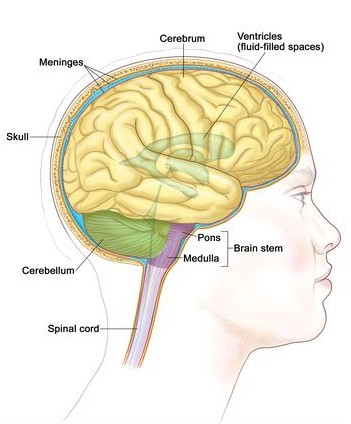
\includegraphics[width=0.55\textwidth]{brainanatomy.jpg}
    \caption{Depiction of some key regions of the brain reproduced from~\cite{Institute2023}.}
    \label{fig:anatomybrain}
\end{figure}
There are also different types of brain cells in which the tumour can originate. The brain contains many neurones which transport the electrical signals that allow the brain to operate. These are surrounded by glial cells, of which there are different types which each play a role in supporting and protecting the neurones~\cite{TheBrainTumourCharity2023}. The main types are astrocytes, oligodendrocytes and ependymal cells. When the tumour originates in glial cells it is termed a glioma with subcategories corresponding to each type of glial cell. Astrocytomas, originating in astrocytes, are the most common gliomas with the different grades given different names such as Grade 4 astrocytoma named glioblastoma multiforme~\cite{BrainTumourResearch2023}. Similarly, oligodendrogliomas originate from oligodendrocytes, and ependymomas originate from ependymal cells~\cite{TheBrainTumourCharity2023}. %include meningioma lymphoma medulloblastoma adenoma \\

There are over 130 types of brain tumours as classified by the World Health Organisation (WHO) and differ in terms of which type of cell they originate in, their grade, and which part of the brain they affect.

\subsection{Current treatments}\label{sec:introtumourtreatments}
Initially or if no other treatment options are possible, the symptoms of a brain tumour can be treated without treating the tumour itself, for example anti-sickness medication to treat the nausea. The treatment plans are determined based on a number of factors which include the type, location, and grade of the tumour as well as the patient's overall health~\cite{NationalHealthService2023}. Surgery is a preferred treatment where possible as it is possible to remove a large proportion, if not all, of the tumour with this method. In cases where the full tumour may not be removed, such as when there is a significant infiltration zone into surrounding healthy tissue where the border of the tumour is challenging to identify, this may be followed up with radiotherapy or chemotherapy. These treatment options can also be used separately when surgery is not an option~\cite{MacmillanCancerSupport2019}. 

Neurosurgical resection aims for maximum safe resection of the tumour which balances a high extent of resection while preserving functional regions of brain as improved resection is linked to improved patient outcomes~\cite{Chanbour2022}. To this end a variety of techniques can be employed to improve resection. These include: a surgical microscope which enables clear visualisation of the surgical field, neuronavigation which allows registration of a probe against an MRI, awake or asleep sub-corticol mapping to allow identification of eloquent areas of brain, in some cases fluorescence imaging using 5-aminolevulinic acid (5-ALA) or indocyanine green (ICG) can be used for tumour localisation, and microvascular doppler (MVD) or ICG can be used for tumour vessel localisation~\cite{Chanbour2022, Catapano2018}.

Whilst these these adjuncts have improved the quality of tumour resection, they are associated with some limitations~\cite{Chanbour2022}. Neuronavigation reduces in accuracy as the anatomy changes throughout a procedure, known as brain shift. Whilst this can be counteracted using intra-operative MRI, this disrupts surgical workflow and has large associated costs~\cite{Chanbour2022}. Sub-cortical mapping allows identification of eloquent regions of brain, however this does not provide a spatially-resolved tumour boundary and carries risks of intraoperative seizures or postoperative emotional distress~\cite{Chanbour2022}. Label-based methods such as fluorescence utilising 5-ALA or ICG can be effective but are limited by the label behaviour and the type of tumour in which it is effective~\cite{Chanbour2022}. For example, fluorescence imaging has been shown to have limited application in low grade glioma resections due to the low aggregation of fluorophore in these less aggressive tumours~\cite{Belykh2023, Kiesel2021, Jaber2019}. Vessel localisation may also be effective with MVD or ICG displaying the flow of blood, however this is unable to quantify the oxygen saturation of this blood or verify the oxygen transfer into tissues which introduces an element of subjectivity into tissue viability assessment. Even the widely adopted surgical microscope can be associated with operator fatigue and its maneuverability is limited by its size~\cite{Alamer2023}. Exoscopes have been proposed to address these challenges, however these are associated with potential learning curves for new users~\cite{Alamer2023}.

Where these techniques have been used they have improved patient outcomes while demonstrating some key features that aid in surgical integration. The introduction of real-time visualisation with a high spatial resolution from the surgical microscope has lead to improvements in maximal safe tumour resection~\cite{Alamer2023}. For this reason, fluorescence imaging and ICG have been incorporated into such devices to make use of these properties. These techniques illustrate the importance of tools that enable accurate distinction between healthy and cancerous tissues for safe resection~\cite{Belykh2023}. These features are all present in intra-operative MRI, however its limited adoption draws attention to the importance of ensuring technological advancements integrate well with the surgical workflow. The detrimental impact of brain shift on the quality of neuronavigation demonstrates the importance of real-time evaluation to ensure all information presented is accurate for the anatomy onto which it is applied~\cite{Alamer2023}. The importance of vessel visualisation is also seen in the applications of ICG where this allows for tumour feeding and peritumour vessels to be visualised enabling improved retention of normal anatomy post-resection~\cite{Catapano2018}. This demonstrates the need for real-time, spatially-resolved, visualisation of tumour boundaries and vascularisation intra-operatively. Whilst many existing clinical adjuncts address subsets of these properties, HSI presents potential to address all of these.  

\section{Brain aneurysms}\label{sec:aneurysms}
Another key set of conditions addressed by neurosurgery include brain aneurysms. These are a subset of all aneurysms which are balloon-like abnormal dilatations in a vessel wall due to a weakness caused by high blood pressure, smoking, or genetic predisposition~\cite{NationalHealthService2022}. Most aneurysms will only have significant symptoms on rupturing which is called a subarachnoid haemmorhage and can cause extensive brain damage as well as blinding headaches, sickness, or pain looking at light~\cite{NationalHealthService2022} with approximately 500,000 people dying annually~\cite{Toth2018}. 

\subsection{Current treatments}\label{sec:introaneurysmtreatments}
Treatment of unruptured aneurysm is determined by risk of rupture, size, and location in the brain. If the aneurysm is considered to have a low risk of rupture, treatment may focus on limiting risk factors~\cite{NationalHealthService2022}. In ruptured aneurysms or those at higher risk of rupturing, however, treatment is primarily surgical in the form of clipping or endovascular procedures depicted in Figure \ref{fig:aneurysmtreatment}. The former involves the placement of a metal clip over the opening to prevent further blood flow into the aneurysm~\cite{TheBrainFoundation2023}. Endovascular procedures can include coiling to encourage clotting in the aneurysm to prevent further blood flow, which can be combined with further devices including stents to hold the coil in place~\cite{TheBrainFoundation2023}. The final endovascular technique is flow diversion achieved by placing a cylindrical tube (similar to a stent with a tighter weave) in the vessel over the aneurysm opening to allow normal blood flow~\cite{TheBrainFoundation2023}. 
\begin{figure}[h]
    \centering
    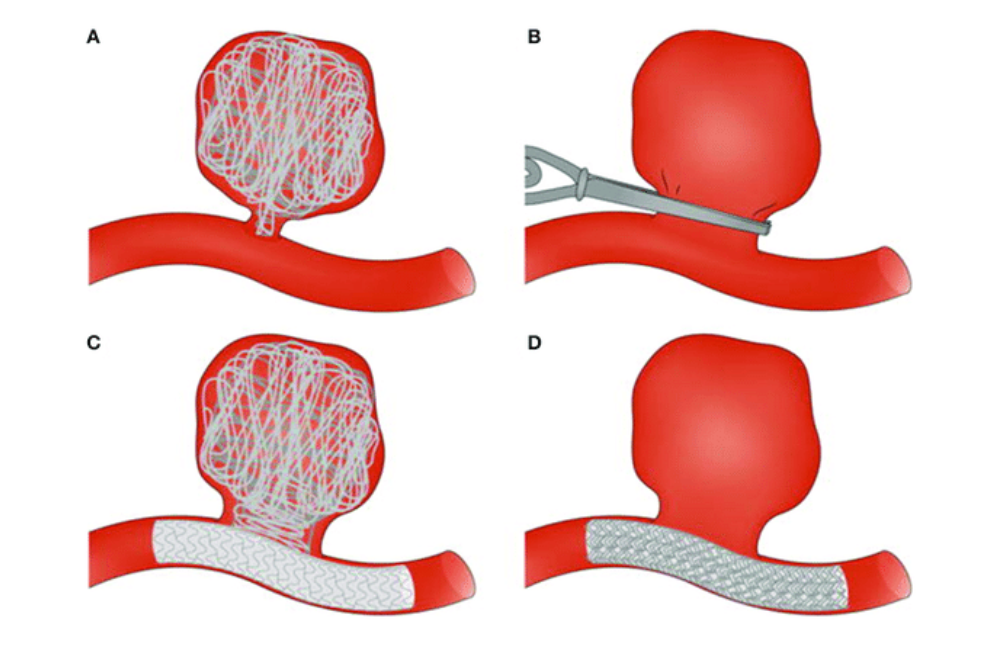
\includegraphics[width=0.9\textwidth]{Aneurysm-treatments.png}
    \caption{An illustration of some key surgical treatment methods for brain aneurysms reproduced from~\cite{TheBrainFoundation2023} where the technique depicted by A is coiling, B is clipping, C is coiling combined with a stent, and D is flow diversion.}
    \label{fig:aneurysmtreatment}
\end{figure}
Whilst these treatment methods are often very effective, incomplete aneurysm occlusion can lead to rupture at a later date with the extent of occlusion being linked to the likelihood of this occurring~\cite{Toth2018}. For this reason blood flow is often assessed intra-operatively using digital subtraction angiography (DSA), MVD, or ICG~\cite{Norat2019}. DSA is produced by subtracting an X-ray image taken without a contrast agent from one taken with a fluorescent contrast agent to visualise only the vessels in the field of view~\cite{Radiopia2022}. This can be done intra-operatively to visualise the blood flow, however the gold-standard for determining quality of aneurysm occlusion is a post-operative DSA~\cite{Marbacher2020}. DSA cannot be used continuously intra-operatively due to the changing geometry, the complex procedure for DSA aquisition, and the radiation dose risk~\cite{Radiopia2022, Derdeyn1999}. ICG provides a real-time alternative to DSA, however it also requires a fluorescent dye and is of lower precision~\cite{Norat2019, Anania2023}. MVD is also able to determine if full occlusion has occurred intra-operatively and has the advantage of not requiring a labelling agent, however this technique is highly subject to angle and depth~\cite{Anania2023}. Additionally, temporary clipping of healthy vessels can be used to control intra-operative bleeding, however this may lead to cerebral ischaemia where tissues have limited access to oxygenated blood~\cite{Doron2022}. 

Similarly to those in Section \ref{sec:introtumourtreatments}, the advantages of the current clinical adjuncts provide valuable information of the desirable features in technology to aid aneurysm treatment. DSA, ICG and MVD all demonstrate the desirability of spatially-resolved evaluation technique. DSA and MVD highlight the importance of accounting for changing geometry or imaging position, while ICG draws attention to the advantage of label-free techniques. While ICG can distinguish oxygenated blood flow, there are also no clinically available techniques to determine tissue oxygenation status. For this reason a real-time, intra-operative, spatially-resolved, quantitative measure of oxygen saturation which can be applied to both vessels and tissues in a range of imaging geometries is desired. HSI has been shown to address many of these challenges with steps towards the geometry-invariant imaging being addressed in this work. 

\section{Oxygen saturation}\label{sec:oxygensat}
As discussed in the previous sections, Oxygen saturation is proposed to be a useful parameter in neurosurgical decision making. Additionally, cerebral ischaemia is known to have debilitating consequences with limited intra-operative monitoring options~\cite{Zhou2016}, for this reason investigating $StO_2$ evaluation is considered a key physiological parameter for research in this work. 

Oxygen is required by all cells in the body to release energy by respiration. This oxygen is transported to cells by haemoglobin, primarily in the red blood cells of blood, which can take the forms of oxyhaemoglobin and deoxyhaemoglobin based on whether the haemoglobin is bound to oxygen or not respectively. These forms of haemoglobin have very different absorbance characteristics as seen in their extinction spectra in Figure \ref{fig:Haemoglobinext}. 
\begin{figure}[h]
    \centering 
    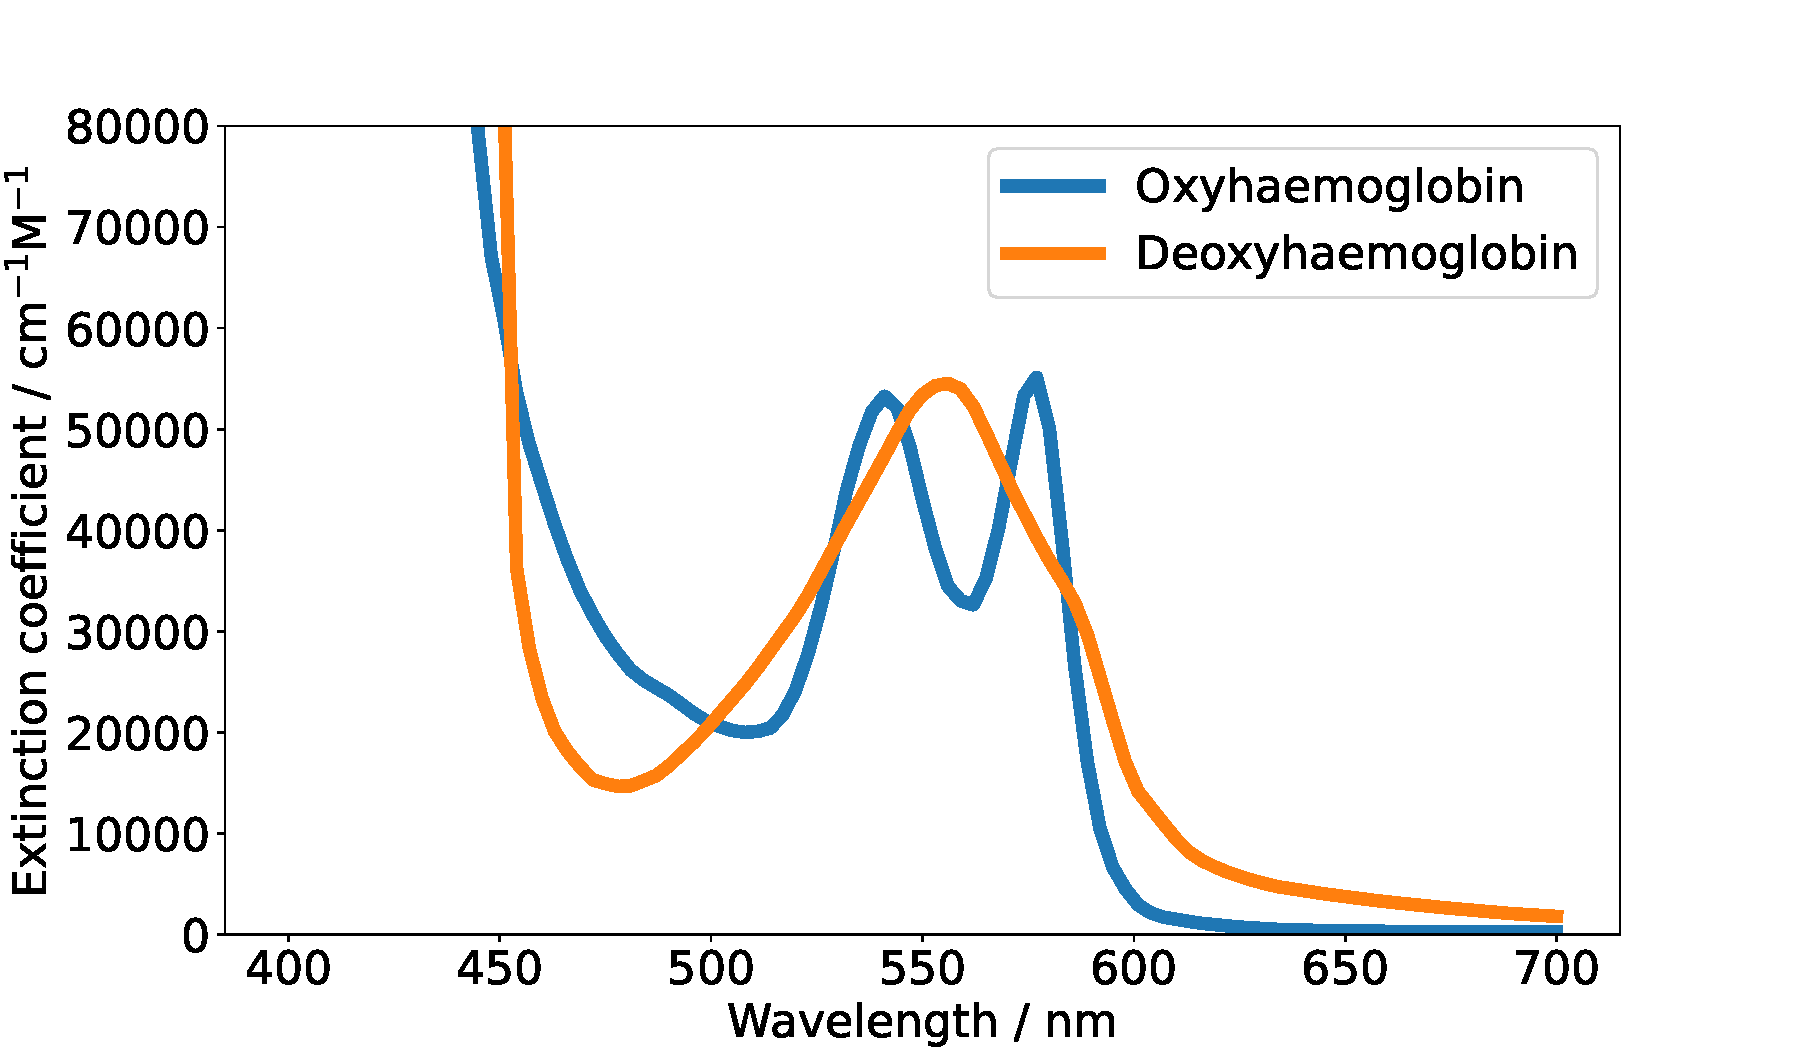
\includegraphics[width=0.7\textwidth]{Hb_eps.pdf}
    \caption{The extinction coefficients for oxyhaemoglobin and deoxyhaemoglobin reproduced from~\cite{Prahl1998}.}
    \label{fig:Haemoglobinext}
\end{figure}
Oxygen saturation is defined as the proportion of haemoglobin which is oxygenated ie $\frac{HbO_2}{HbO_2 + Hb}$ where $Hb$ is deoxyhaemoglobin and $HbO_2$ is oxyhaemoglobin. 

There are no currently established, intra-operative, techniques to assess $StO_2$ in neurosurgery and so perfusion is often used as an indicator instead with DSA, MVD, and ICG capable of this as detailed in Sections \ref{sec:introtumourtreatments} and \ref{sec:introaneurysmtreatments}. Additionally, there has been significant research into using Laser Speckle Contrast Imaging (LSCI) to visualise blood perfusion, however this is not able to distinguish between $Hb$ and $HbO_2$~\cite{Dunn2012, Zhong2021}. Peri-operative neural monitoring can use jugular venous oxygen saturation (JVOS)~\cite{Raith2020} and cerebral oximetry~\cite{Lian2020} to provide indications of the health of the organ. Both techniques usually make use of near infra-red (NIR) spectroscopy to distinguish between $Hb$ and $HbO_2$. These techniques, however, lack specificity so local regions of ischaemia can be present when these values are within the bounds of normality~\cite{Raith2020, Zhong2021}.

Due to this lack of available techniques, there have been many proposed methods to extract $StO_2$ from tissue diffuse reflectance spectra. These range from the simplest ratiometric two-wavelength methods to more sophisticated analytical models~\cite{MacKenzie2018} or deep-learning based approaches~\cite{Ayala2023}. Using two or three wavelength models can provide good results but require data to be captured at these precise wavelengths placing large constraints on the measurement devices used and significant model assumptions, whereas analytical models can be applied to ranges of wavelengths for which they are developed. Alternatively, Monte Carlo methods are an established approach to modelling light-tissue interaction for a range of wavelengths. It is, however, computationally challenging to apply in an inverse problem setting making the estimation of optical properties from tissue spectra non trivial on the basis of Monte Carlo simulations alone. To obtain the diffuse reflectance spectra intra-operatively, these techniques primarily use HSI which enable non-contact imaging with minimal change to surgical workflow. 

\section{Current state of the art of $StO_2$ measurement}\label{sec:stateofart}
The challenges presented in current neurosurgical practice present an interesting area for development. Many technologies are being developed to address the need for $StO_2$ assessment intra-operatively for these applications. In this section some key research technologies are presented alongside their limitations and the choice to pursue HSI in this work is justified. 

\subsection{Optical coherence tomography}
Optical Coherence Tomography (OCT) is a non-contact 3D imaging modality which provides both spatial and depth information of the tissue imaged. The technique utilises a reference beam and a sample beam; the backscattered light from the sample beam forms an interference pattern with the reference beam which is measured. Traditionally, the mirror used to produce the reference beam is adjusted until interference is maximised, and at this point the distance between the positions of the mirror and sample provides information on the depth of the scatterer. To increase efficiency, the mirror location is fixed and Fourier Transforms are used to analyse the returned interference and provide the depth of the scattering structures at the spatial location measured~\cite{Fercher2003}. By scanning the focussed beam across the sample tissue, a 3D image with both spatial and depth information can be constructed~\cite{Fercher2003}. Traditionally OCT utilises near-infrared wavelengths (NIR) due to the deeper penetration into biologically tissue, however recent advances have shown that using visible wavelengths allows oxygen saturation of vessels to be computed~\cite{Shu2017}. It has also been shown that tumour margins can be highly accurately delineated from this type of data using automated algorithms~\cite{Sunny2019}. 
%Whilst this provides spatially resolved oxygenation information of major vessels, significant attenuation is required for this calculation limiting its application to tissue directly~\cite{Shu2017}. 
This technique allows spatially-resolved, intra-operative, oxygen saturation measurement of vessels and tumour margin delineation using probes that integrate easily into the surgical workflow~\cite{Jansen2018}. Despite these key advantages of OCT, it is also associated with some significant limitations. While OCT is highly suited to measuring oxygen saturation of vessels, significant attenuation of the sample beam is required for this calculation which limits its application to tissue directly~\cite{Shu2017}. Additionally wide-field OCT obtained by scanning the focussed sample beam over the imaging area can provide good spatially-resolved information, however this is subject to motion artefacts of the tissue under examination and limits real-time wide-field implementation~\cite{Yu2015}. These limitations are significant in the context of neurosurgery where local tissue ischaemia is of significant concern and wide-field imaging provides important information for decision-making. 

\subsection{Raman spectroscopy}
Raman spectroscopy is a technique that observes wavelength shifts of laser light due to inelastic molecular scattering. These shifts correspond to vibrational modes of the scattering molecules which enables the chemical composition of the sample to be identified~\cite{Kong2015}. This technique has been combined with multivariate classification models to identify tumour margins primarily in brain and breast cancer surgeries and has recently overcome many of the challenges to its adoption including acquisition speed and accuracy~\cite{Kong2015, Fitzgerald2022}. There have also been advances in the use of this technique for oxygen saturation measurement by measuring resonant peaks of haemoglobin in the far infrared wavlengths, however this is limited to measurement of the oxygen saturation in vessels and requires calibration with blood samples of known oxygen saturation which is highly complex and disruptive to surgical workflow~\cite{TorresFilho2016}. Despite highly accurate intra-operative tissue differentiation being achieved on a cellular level~\cite{Fitzgerald2022}, another key limitation is the lack of wide-field intra-operative applications of this technology. Finally, this technique is highly sensitive to the measurement configuration limiting its clinical application where these configurations can be highly variable. This includes the lighting used in the operating theatre which can confound the results of Raman measurements so particular attention must be paid to the design of these probes to ensure these effects are limited~\cite{Horsnell2016}, and appropriate calibrations must be used which can be disruptive to workflow~\cite{TorresFilho2016}.

\subsection{Probe-based diffuse reflectance spectroscopy}
Diffuse reflectance spectroscopy measures diffusely scattered light from a sample in order to gain information on the absorbance and scattering properties of this sample. Whilst this work focuses on HSI as a method of diffuse reflectance spectroscopy, there are many fibre-optic probe-based systems for these measurements. These systems provide highly accurate diffuse reflectance spectra in a point-based measurement, however they do not provide wide-field imaging~\cite{Nishidate2015}. 
%This limitation, however, can be overcome by stitching together measurements from multiple probe locations~\cite{Thrapp2020}. 
Whilst this technique traditionally involves contact between the probe and the sample, this contact can alter optical properties of the sample so non-contact solutions have been developed which make use of lenses and remove the impact of specular reflections using polarising filters~\cite{Bish2011, Zhu2012}. None of these measurement configurations, however, provide wide-field information. Diffuse reflectance spectroscopy has shown potential for tissue differentiation~\cite{Skyrman2022} and $StO_2$ measurement~\cite{Fredriksson2020} using methods that are also applied to HSI and so are discussed more thoroughly in the following section. These techniques are able to provide real-time, intra-operative, highly accurate measurements which show promise for tissue differentiation and $StO_2$ measurement, however they do not provide wide-field imaging and non-contact configurations introduce significantly more bulk to the system. For this reason HSI is investigated to overcome these limitations. 

\subsection{Hyperspectral imaging}
Hyperspectral imaging (HSI) measures diffuse reflectance spectra using multiple channels, which are narrow spectral measurements centred around a given wavelength. In comparison, traditional imaging only collects three broad channels to create a conventional RGB (red, green, blue) image. HSI provides higher spectral resolution than traditional imaging whilst maintaining a wide field of view. This technique can also be referred to as multispectral imaging when there is a low number of bands, however for simplicity we will refer to this as HSI in all cases~\cite{Clancy2020}. 

HSI is widely used in many applications and has shown promise for medical imaging~\cite{Lu2014,Giannoni2018,Calin2014,Shapey2019}. The ability to measure diffuse reflectance spectra with spatial resolution allows much more information to be displayed in a single acquisition than probe-based alternatives. This allows both spatial and spectral information to be interpretated, computationally or visually, simultaneously which may provide further insights~\cite{Seidlitz2022}. Similarly, the increased spectral resolution may allow for computation of clinically relevant physiological parameters, such as chromophore concentrations, which cannot be determined from traditional RGB imaging so reducing subjectivity~\cite{Seidlitz2022}, and enables computation for tissues directly in addition to examining vasculature. Additionally, HSI is a non-invasive, non-contact imaging modality which can be used in a compact format with minimal disruption to workflow~\cite{Thoenissen2023, Ebner2021, MacCormac2023}. Whilst there are traditionally non-sterile steps required for calibration of these measurements, we address these in Chapter \ref{chap:SWB}. Despite the increased data storage and computational requirements for the large quantities of data associated with HSI~\cite{Altamimi2022}, these advantages suggest that HSI could be a useful tool to elucidate physiological parameters intra-operatively. 

There are three major categories of HSI cameras: spatial scanning, spectral scanning, and snapshot acquisition. Spatial scanning collects data for all wavelengths simultaneously and scans through pixels sequentially, these can be sub-categorised by the scanning order such as linescan or pointscan. Spectral scanning, however, acquires data for all pixels simultaneously and scans through wavelengths sequentially. These methods both capture data consisting of two spatial and one spectral axes directly, forming a full hypercube. For both spatial and spectral scanning methods, the acquisition time is limited by the scanning time and this could lead to motion artefacts in the resulting hypercube and so snapshot implementations have been proposed to address this. The most common of these is snapshot mosaic imaging which acquires one channel per pixel in a single shot~\cite{Geelen2014} with the remaining data inferred by classical or learning-based~\cite{Li2021} interpolation (demosaicing) to construct a full hypercube. Following this demosaicing step, a spectral cross-talk correction must be performed as these systems suffer from parasitic neighbouring channel effects~\cite{Pichette2017}. This methods requires a compromise between spatial and spectral resolution where the number of spectral bands is limited in order to preserve spatial resolution. An alternative method is Coded Aperture Snapshot Spectral Imaging (CASSI) which utilises image compression tools to obtain a 2D acquisition where each pixel carries a combination of spectral and spatial information which can be decoded to produce a full hypercube measurement directly~\cite{Song2022, Eldar2009}. This method has not yet been applied intra-operatively as integration has proved challenging due to the significant increase in required optical components compared to traditional HSI approaches, and the requirement for detailed calibration of these to enable high spatial resolution reconstruction with reconstruction algorithms that are complex and computationally intensive~\cite{Song2022}. An alternative method to capture the whole hypercube in a single shot is lightfield HSI which uses a large sensor and a microarray of lenselets each with their own spectral filtering that is dependent on the angle of light. This results in an image where each pixel location corresponds to a different wavelength dependent on the lenselet projected to that position and the angle of detected light. This allows for high spectral resolution and has also shown high spatial resolution in controlled testing, however this has not yet translated to high intra-operative spectral resolution which is limited by the complex parallax correction required for a non-planar anatomical surface in addition to any motion here causing artefacts~
\cite{MacCormac2023}.  

Whilst spatial and spectral scanning methods have been used for most medical applications to date due to their high spectral quality, they often require long acquisition times and may be prone to motion artefacts~\cite{Kulcke2018, Giannoni2021, Shapey2019, Yoon2021}. Snapshot acquisition methods, however, allow for real-time imaging which provides improved clinical integration~\cite{Ayala2021, Ebner2021}. Since we consider spatial resolution to be of key importance for surgical guidance, we utilise snapshot mosaic imaging for this work which is depicted alongside spatial and spectral imaging methods in Figure \ref{fig:scanning}.
\begin{figure}[h]
    \centering
    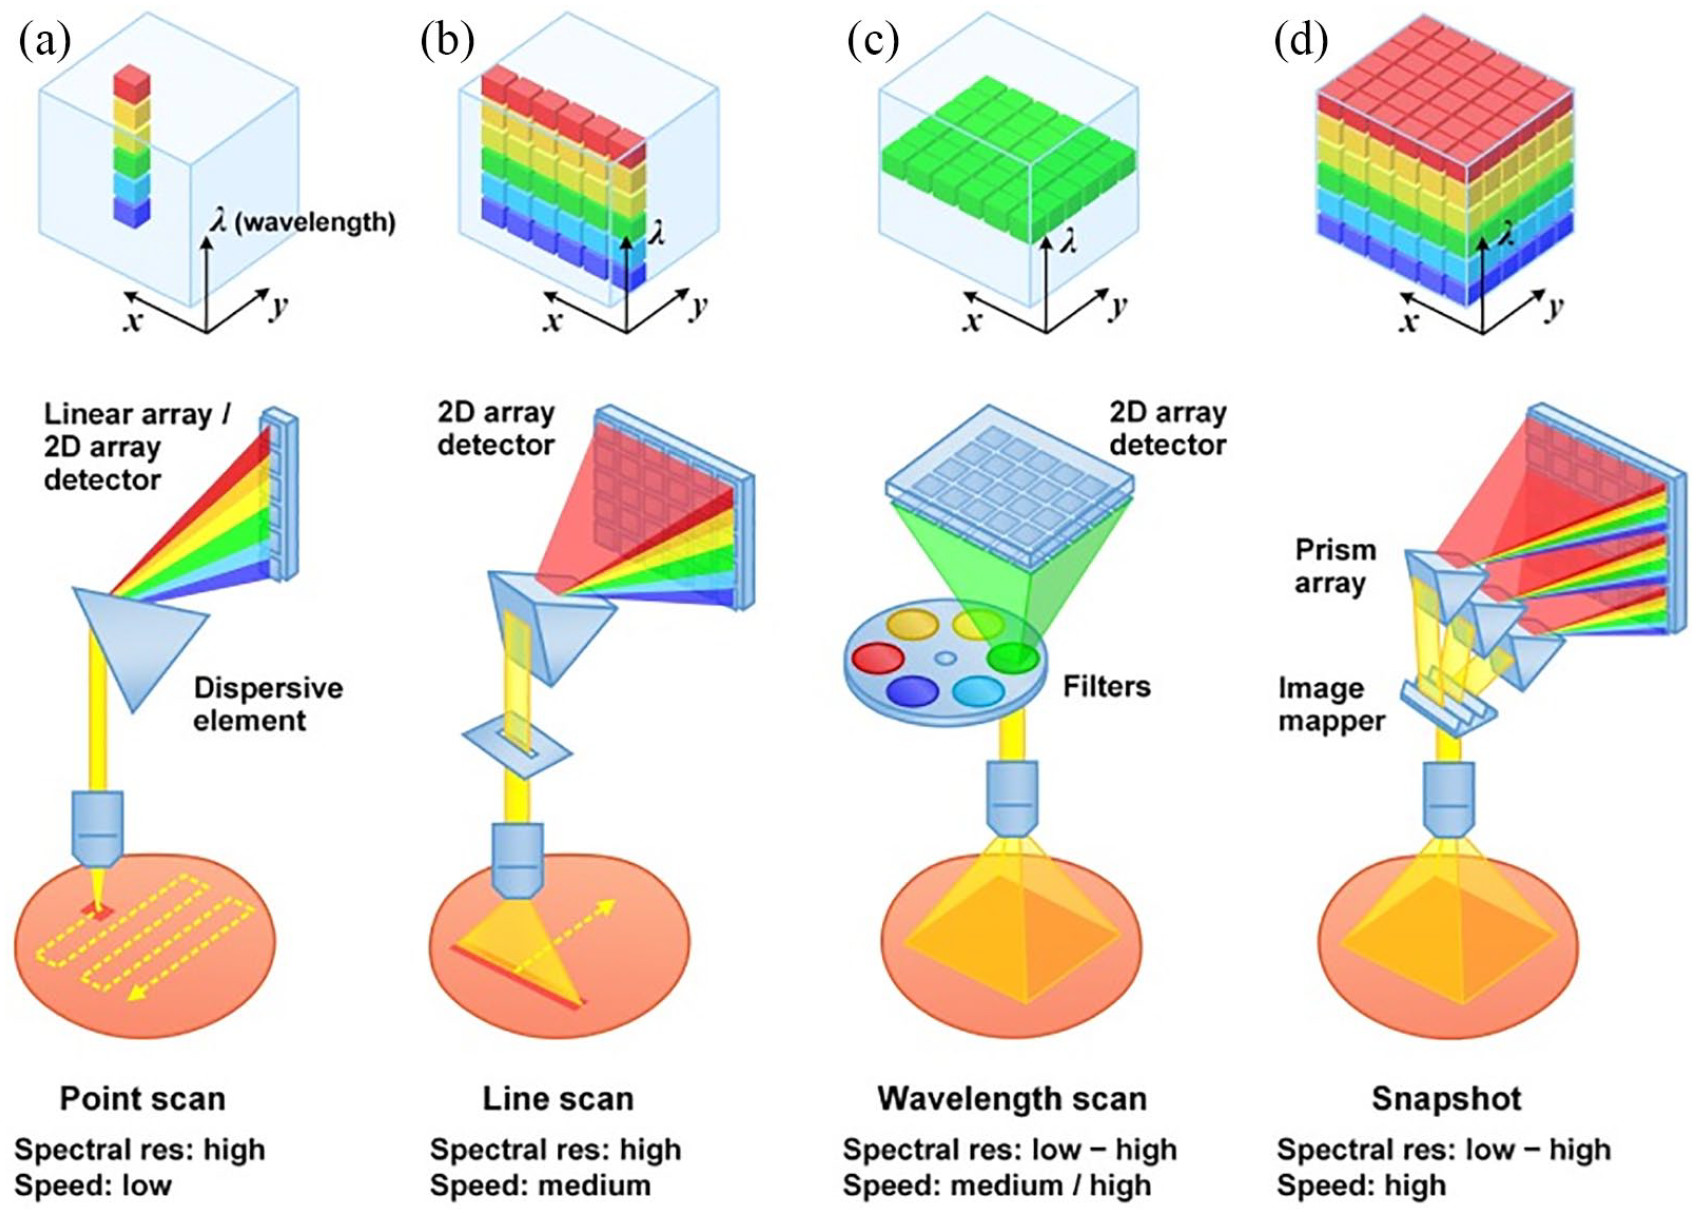
\includegraphics[width=0.7\textwidth]{scanning_types.jpeg}
    \caption{Depiction of the major HSI acquisition methods reproduced from \cite{Araujo-Andrade2021}. Note that here the snapshot acquisition result is depicted after demosaicing.}
    \label{fig:scanning}
\end{figure}

In all cases, and traditional imaging, an initial white-balancing step must be used to account for lighting conditions, vignetting, and optical transmission through the set-up. This step traditionally uses a white and dark reference, where the white reference is an image of a uniform, highly reflective, Lambertian surface~\cite{Lu2014}. This step should be repeated for any change in imaging configuration to obtain quantitatively accurate spectral data as detailed further in Chapter \ref{chap:SWB}. Whilst these steps traditionally use non-sterile equipment and so are challenging to integrate into surgical environments, we provide a novel sterile approach in Chapter \ref{chap:SWB} to mitigate this limitation. 

Spatial Frequency Domain Imaging (SFDI) can be utilised with HSI to provide accurate, spatially-resolved, sampling depth information by projecting patterns of different frequencies which are either spatially or temporally demodulated~\cite{Gioux2019}. Whilst this provides useful additional information, for example for accurate white balancing, this method is disruptive to surgical workflow and so is not utilised in this work. 

Throughout this thesis a snapshot HSI camera with a 4x4 mosaic pattern across the sensor (Ximea utilising the IMEC CMV2K-SSM4X4-VIS sensor, Germany) is chosen which enables fast data acquisition and integration into a variety of imaging configurations. This sensor is combined with an f=35mm coupler (Karl Storz, NDTec, VCam HD-F-35 - Camera Lens Adapter, Germany) and an exoscope (Karl Storz Endoscopy, VITOM Telescope 0° w Integ. Illuminator, UK) for imaging. This creates a standalone imaging system which is combined with various light sources. In this work, this system is used in a highly controlled manner either mounted to a seven degree of freedom robot (LBR, KUKA med7 R800, Germany) to enable multiple images to be taken with a constant reproducible camera position relative to the subject, or mounted to an optical breadboard to ensure fixed camera position, both of which can be seen in Figure \ref{fig:HSIsetups}. This system, however, is also being adapted for clinical use with the use of sterile drapes and a handheld configuration, detailed in Chapter \ref{chap:SWB}. %~\cite{Budd2023}. 
\begin{figure}[h]
    \centering 
    \begin{subfigure}[ht!]{0.27\textwidth}
	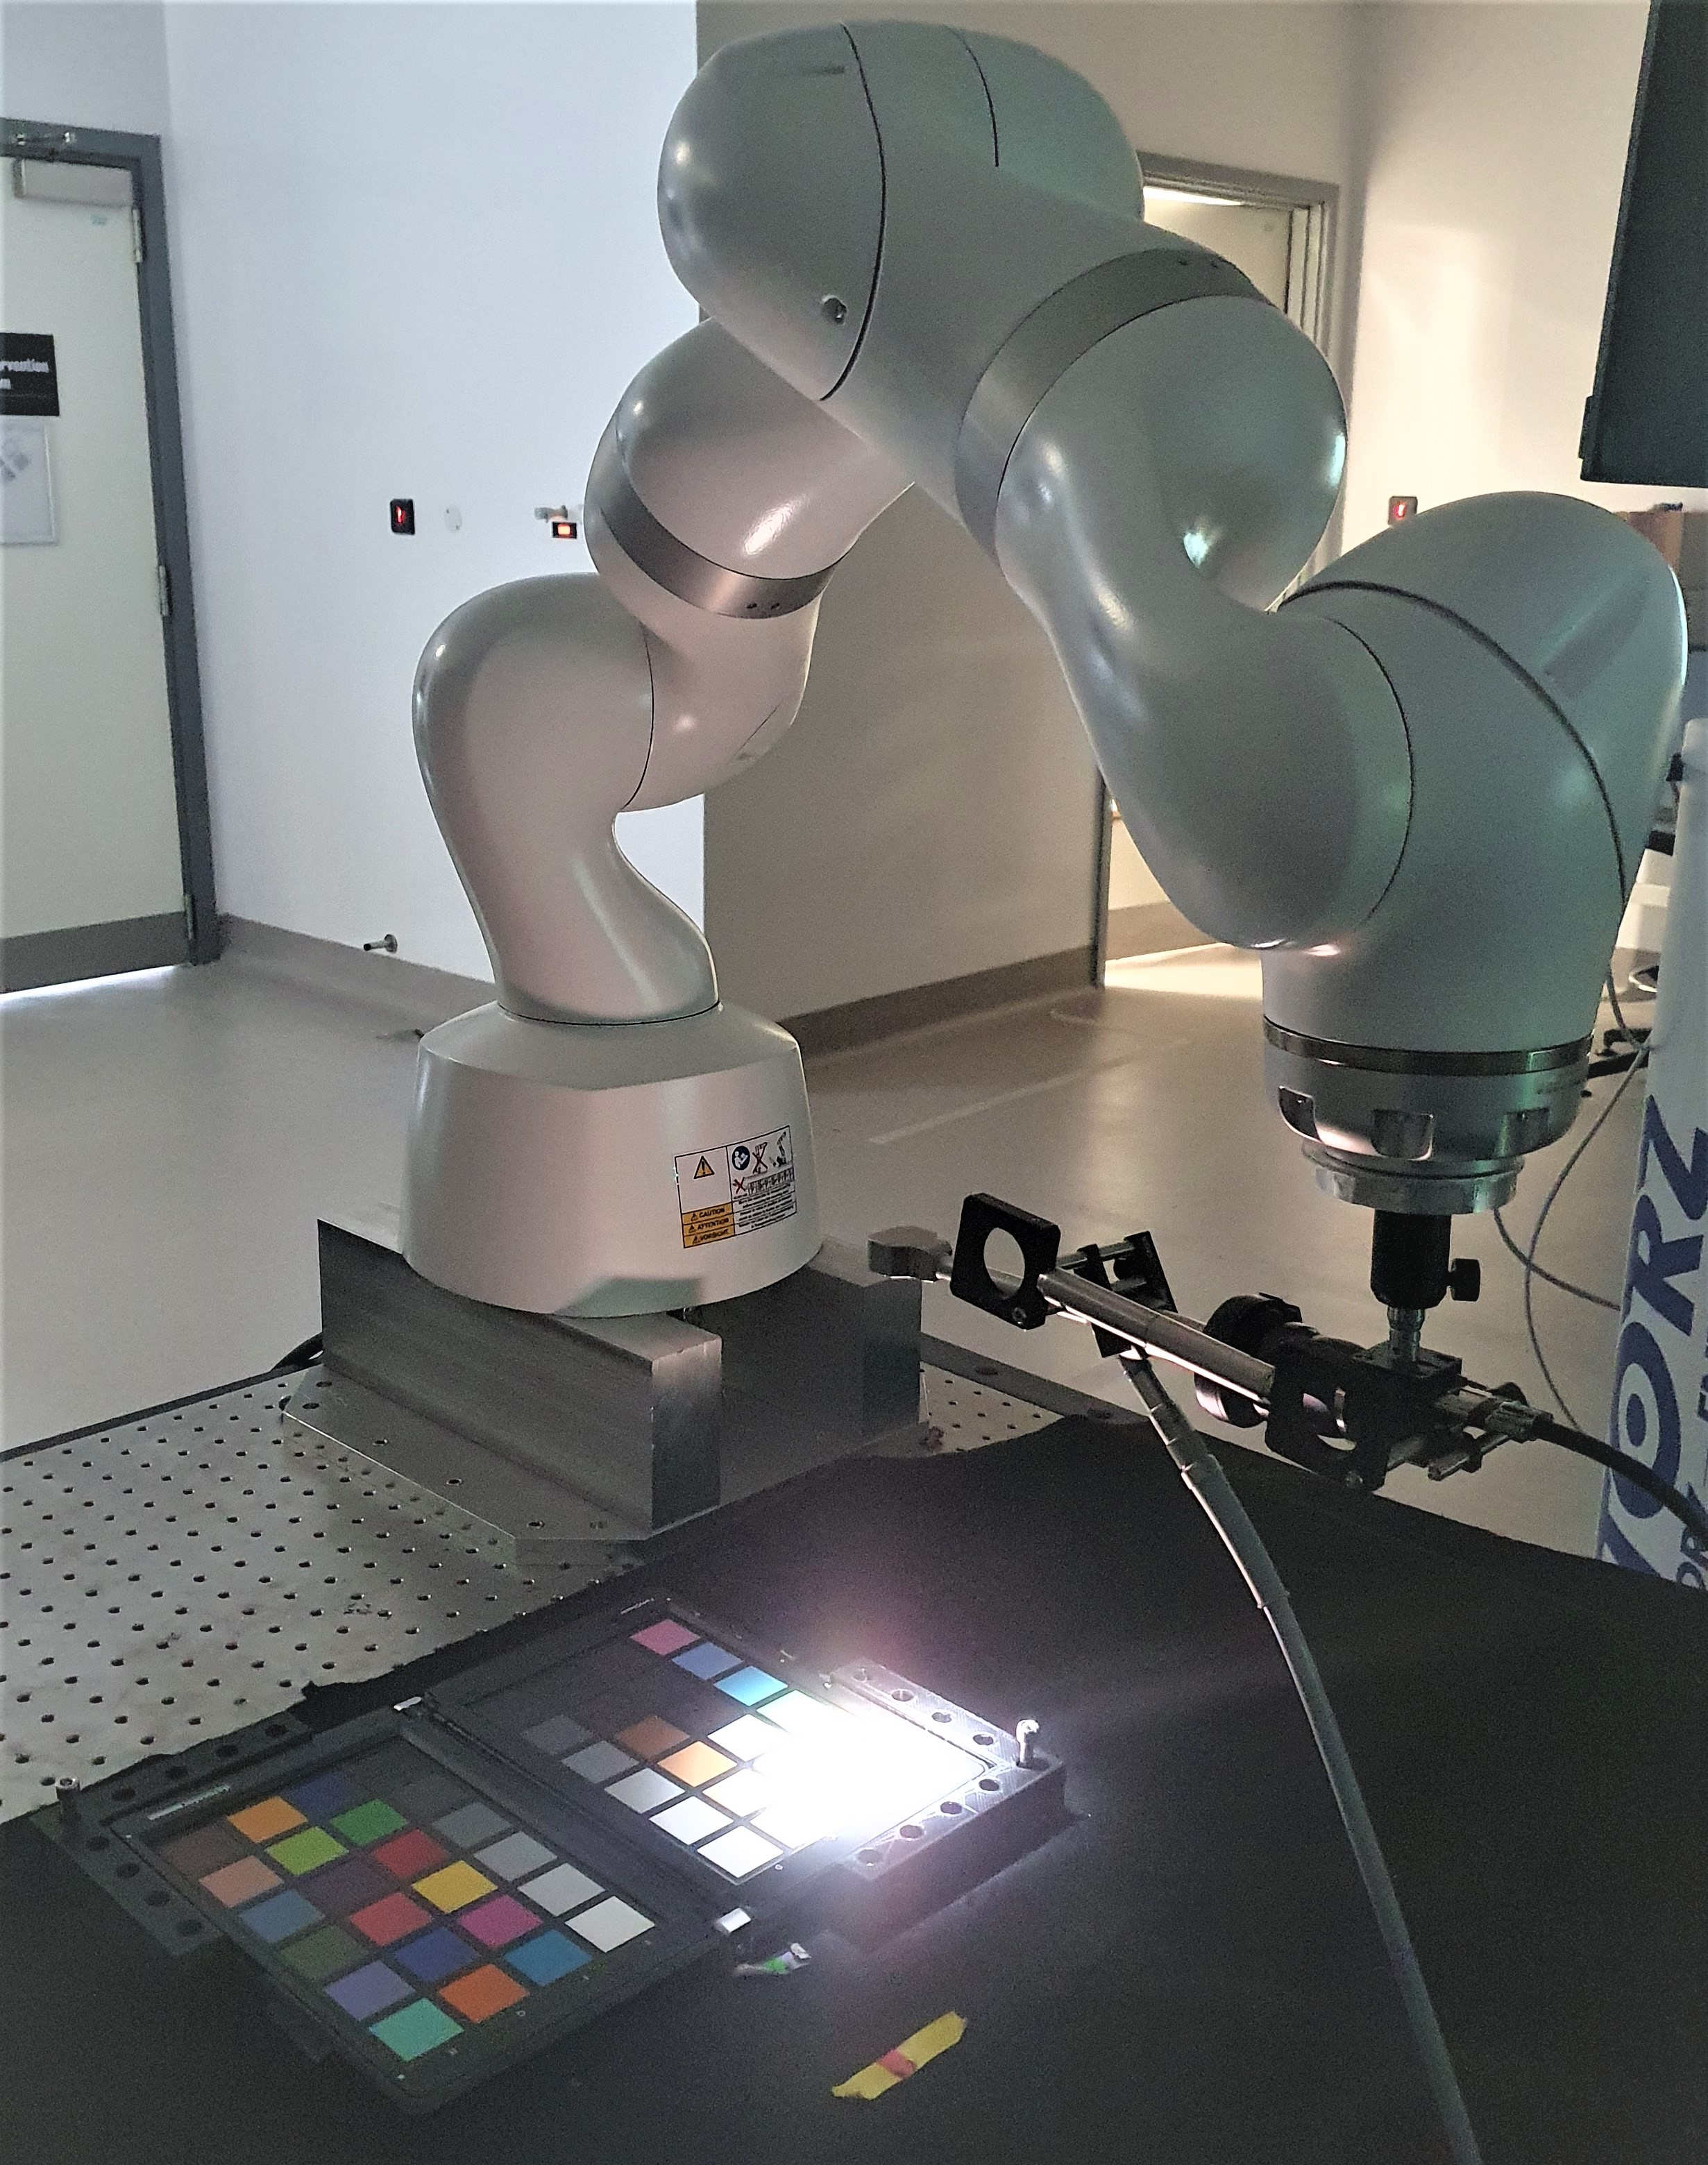
\includegraphics[width=\textwidth]{KUKAHSI}
	\caption{}
	\label{fig:KUKAHSI}
    \end{subfigure}
    \begin{subfigure}[ht!]{0.16\textwidth}
        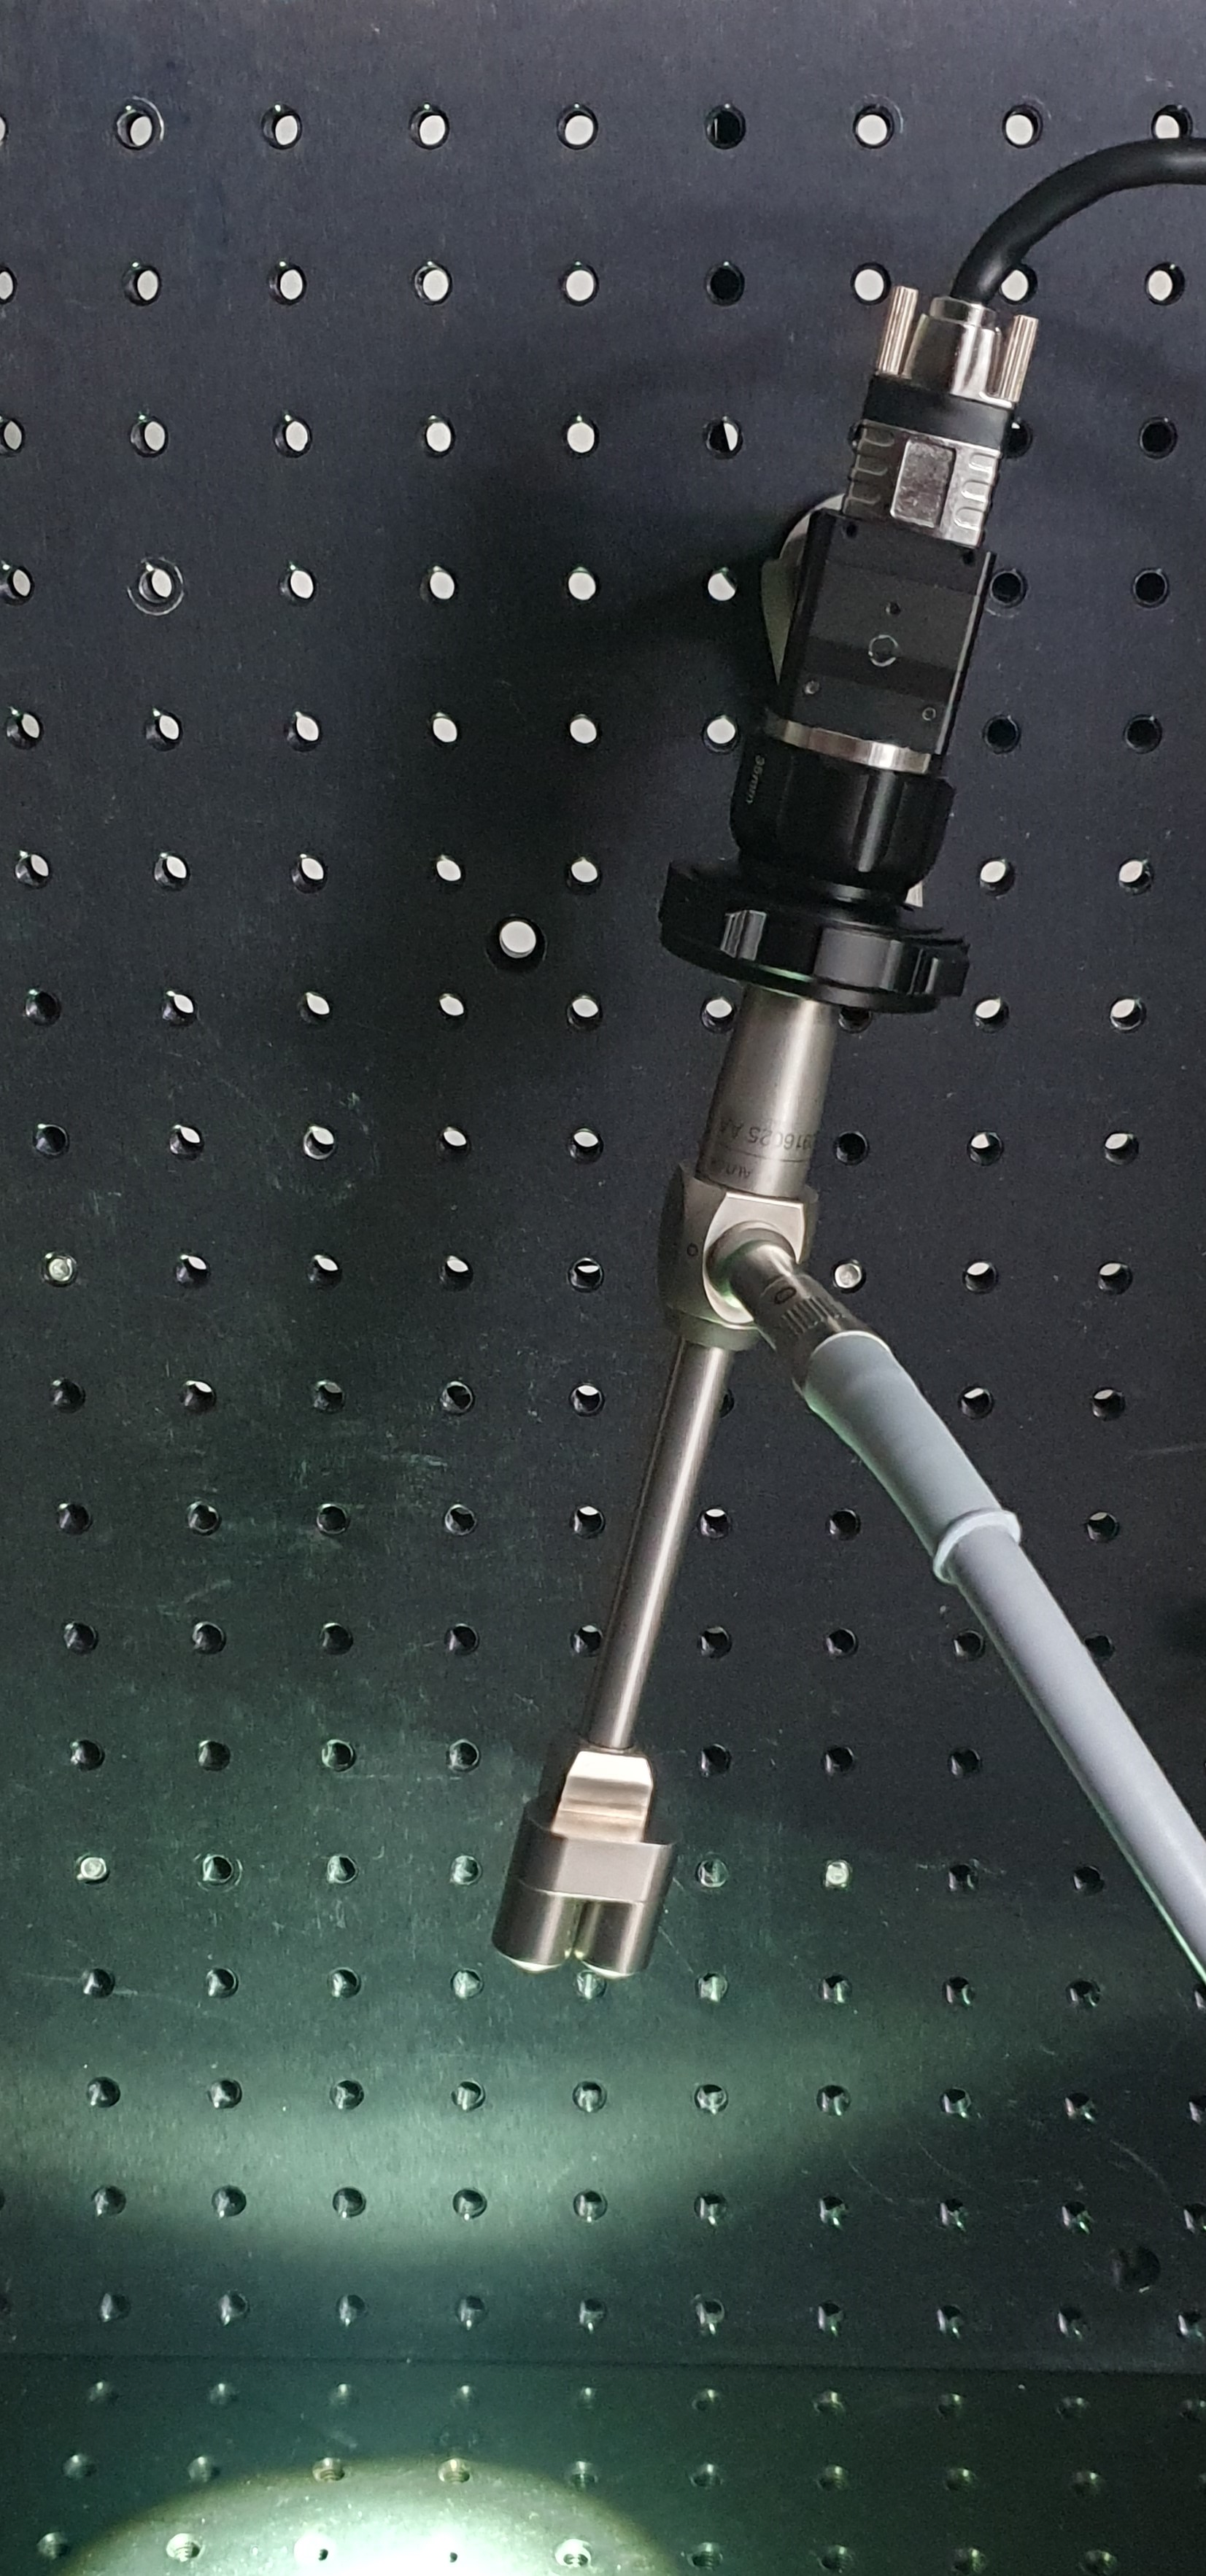
\includegraphics[width=\textwidth]{imagephantoms}
        \caption{}
        \label{fig:ScopeHSI}
    \end{subfigure}
    \caption{Snapshot HSI system comprising the sensor (Ximea utilising the IMEC CMV2K-SSM4X4-VIS sensor, Germany), an f=35mm coupler (Karl Storz, NDTec, VCam HD-F-35 - Camera Lens Adapter, Germany), and an exoscope (Karl Storz Endoscopy, VITOM Telescope 0° w Integ. Illuminator, UK) mounted to a seven degree of freedom robot (LBR, KUKA med7 R800, Germany) (\ref{fig:KUKAHSI}) or a static optical breadboard (\ref{fig:ScopeHSI}).}
    \label{fig:HSIsetups}
\end{figure}
%
%It is hoped that the increased spectral resolution would allow computation of clinically relevant physiological parameters, such as chromophore concentration. These 
It is hypothesised that spatially resolved, clinically relevant, physiological parameters extracted using HSI could aid decision making intra-operatively. Much investigation has already been undertaken into this with tissue differentiation~\cite{Kabwama2016, Fabelo2019, Kho2019, Giannantonio2023} and $StO_2$ extraction~\cite{Yudovsky2015, Clancy2015, WOS:000360241100026, Wirkert2016, Clancy2020, Thoenissen2023} showing great promise from intra-operative HSI data acquisition. 

\section{Outline of thesis}\label{sec:thesisoutline}
In the current chapter I have outlined the principles of HSI and outlined the clinical need for an intra-operative, spatially-resolved, $StO_2$ method alongside the existing technology available for this. 
Chapter \ref{chap:SWB} investigates the necessity for in situ white references and address this by proposing a novel, sterile, synthetic reference construction algorithm. The use of references obtained at different distances and lighting conditions to the subject were examined. Spectral and color reconstructions were compared with standard measurements qualitatively and quantitatively, using $\Delta E$ and normalised RMSE respectively. The algorithm forms a composite image from a video of a standard sterile ruler, whose imperfect reflectivity is compensated for. The reference is modelled as the product of independent spatial and spectral components, and a scalar factor accounting for gain, exposure, and light intensity. Evaluation of synthetic references against ideal but non-sterile references is performed using the same metrics alongside pixel-by-pixel errors. Finally, intraoperative integration is assessed though cadaveric experiments.

Chapter \ref{chap:1layer} compares three analytical optical reflectance models for homogeneous, semi-infinite, tissue that have been proposed (Modified Beer-Lambert~\cite{Clancy2015}, Jacques 1999~\cite{Jacques1999}, Yudovsky 2009~\cite{Yudovsky2009}) which have not previously been directly compared for tissue parameter extraction purposes. I compare these analytical models using Monte Carlo simulated diffuse reflectance spectra and controlled gelatin-based phantoms with measured diffuse reflectance spectra and known ground truth composition parameters. 

In Chapter \ref{chap:2layer} a two layer model (Yudovsky 2009) is evaluated against Monte Carlo simulations and used to analyse a NIST skin reflectance dataset. By focussing on the quality of the oxygen saturation ($StO_2$) recovery, the performance of this model is evaluated across the parameter range and a significant region of failure identified. 

Chapter \ref{chap:HSImodel} investigates the impact of reducing the spectral resolution of the diffuse reflectance data and the introduction of noise by simulating camera responses from simulated and experimental data. This camera simulation is also used to adapt the analytical models for use with snapshot hyperspectral data. The impact of this is evaluated using simulations and gelatin-based phantom data similarly to previous chapters. This is evaluated using mean spectra from annotated regions of HSI images and on a pixel-by-pixel basis to investigate the ability of HSI to provide spatial resolution. Finally, some initial examples of applying these models to intra-operative, hyperspectral, neurosurgical data are shown. 

% \begin{document}
\chapter[Synthetic white balancing]{Synthetic white balancing for intra-operative hyperspectral imaging}
\label{chap:SWB}

\begin{center}
\begin{minipage}[b]{0.9\linewidth}
\small
\textbf{Foreword\,}
This chapter is an \emph{in extenso} reproduction of \citet{Bahl2023} and has formed the basis of patent application 2309106.9. 
\newline
AB identified the separable spatial and spectral model, utilised this to create a synthetic white balancing algorithm, collected the testing dataset of the coloured checkerboard target, and evaluated the algorithm in this contexts under the supervision of TV, MB, and JS. JS identified the sterile ruler as a potential imaging target. AB and OM collected the cadaveric hyperspectral data which was analysed utilising the algorithm by AB. CH developed the sRGB reconstruction algorithms and some of the software toolkit used for data processing. MJ aided AB in the conception of the utilisation of the temporal hypercube in the algorithm, this was then developed by AB. PN developed the core of the software used to capture hyperspectral data. This was combined by AB with the software developed by MH for maneuvering the seven degree of freedom robot. The cadaveric procedure was facilitated by NC and PF as part of the FAROS project funded by the European Union’s Horizon 2020 research and innovation programme under grant agreement No 101016985. The light source spectra were measured by JQ and the spectrometer set-up used for this was developed by YX. 
\end{minipage}
\end{center}

\minitoc

% \begin{comment}
% \author[a, *]{Anisha Bahl}
% \author[a, b]{Conor C Horgan}
% \author[b]{Mirek Janatka} 
% \author[a, c]{Oscar J MacCormac} 
% \author[b]{Philip Noonan} 
% \author[a]{Yijing Xie} 
% \author[a, e]{Jianrong Qiu}
% \author[d]{Nicola Cavalcanti} 
% \author[d]{Philipp F\"urnstahl} 
% \author[b]{Michael Ebner}
% \author[e]{Mads S Bergholt} 
% \author[a, b, c]{Jonathan Shapey}
% \author[a, b]{Tom Vercauteren}
% \ead{anisha.bahl@kcl.ac.uk}

% \affil[a]{School of Biomedical Engineering \& Imaging Sciences, King's College London, 1 Lambeth Palace Road, London, United Kingdom}
% \affil[b]{Hypervision Surgical Ltd, 85 Great Portland Street, London, United Kingdom}
% \affil[c]{King's College Hospital, Denmark Hill, London, United Kingdom}
% \affil[d]{Balgrist University Hospital, Forchstrasse 340, 8008 Zurich, Switzerland}
% \affil[e]{Centre for Craniofacial and Regenerative Biology, King's College London, London, United Kingdom}
% \end{comment}

% \begin{document} 
% \maketitle
% \noindent \footnotesize\textbf{*}Corresponding author,  \linkable{anisha.bahl@kcl.ac.uk} 

% \begin{abstract}
% \section{Abstract}
% \noindent \textbf{Purpose} 

% \noindent Hyperspectral imaging (HSI) has shown promise for surgical applications to non-invasively provide spatially-resolved, quantitative, spectral information. In order to interpret this data, a white reference image of a highly reflective Lambertian surface should be obtained under the same conditions as the subject.
% Standard white reference tiles are not sterilisable, making them unsuitable for use in a surgical environment.
% We demonstrate the necessity for an in situ white reference, and address this need by proposing a novel synthetic reference construction algorithm suitable for use in a surgical setting. 
% \noindent Hyperspectral imaging shows promise for surgical applications to non-invasively provide spatially-resolved, spectral information.
%For which,
% For calibration purposes,
% a white reference image of a highly-reflective Lambertian surface should be obtained under the same imaging conditions.
% Standard white references are not sterilizable, and so are unsuitable for surgical environments.
% We demonstrate the necessity for in situ white references and address this by proposing a novel, sterile, synthetic reference construction algorithm.

% \noindent \textbf{Approach}

% \noindent The effects of using references obtained at different distances or under different lighting conditions relative to the subject were examined qualitatively and quantitatively. Qualitatively, these are evaluated by plotting the spectra against those measured with a spectrometer and using sRGB color reconstructions. Quantitatively, these are measured using $\Delta E$ comparisons between the color reconstructions, and normalised RMSE ($\NRMSE$) comparisons between the spectra. These demonstrate the necessity for an in situ white reference. 
% The algorithm utilizes composite images extracted from a video of the ruler. These are corrected to account for the imperfect reflectivity of the ruler, and modelled as the product of independent spatial and spectral components, as well as a scalar factor to account for gain, exposure, and light intensity. 
% Synthetic references constructed using this method are then evaluated by the same metrics used to identify the need for an in situ reference. Finally, this method is applied to a cadaveric spine surgery. 
% \noindent The use of references obtained at different distances and lighting conditions to the subject were examined.
%These were evaluated by comparing spectra
% Spectral
% and color reconstructions
% were compared
% with standard measurements qualitatively and quantitatively, using $\Delta E$ and normalised RMSE respectively. 
% The algorithm forms a composite image from a video of a standard sterile ruler, whose imperfect reflectivity is compensated for. The reference is modelled as the product of independent spatial and spectral components, and a scalar factor accounting for gain, exposure, and light intensity. 
% %Synthetic references are evaluated by the same metrics alongside pixel-by-pixel absolute percentage errors relative to the ideal, non-sterile, measured.
% Evaluation of synthetic references against ideal but non-sterile references is performed using the same metrics alongside pixel-by-pixel errors. 
% %Finally, this is translated to cadaveric surgery.
% Finally, intraoperative integration is assessed though cadaveric experiments.

% \noindent \textbf{Results}

% % \noindent Improper white balancing leads to an approximate 300\% increase in all quantitative error metrics and visible qualitative spectral and color changes. 
% % Our white reference algorithm consistently achieves median pixel-by-pixel percentage errors of less than 6.5\%  and produces similar spectral reconstructions and errors relative to an ideal measured white reference (unsuitable for surgical use).
% % Applied in cadaveric spine surgery, our algorithm integrated well into the surgical work flow and achieved median absolute pixel-by-pixel errors of 4.77\% relative to an idealized white reference, while maintaining good spectral and color reconstruction fidelity.
% \noindent Improper white balancing leads to increases in all quantitative and qualitative errors. 
% Synthetic references achieve median pixel-by-pixel errors lower than 6.5\%  and produce similar reconstructions and errors to an ideal reference.
% The algorithm integrated well into surgical workflow, achieving median pixel-by-pixel errors of 4.77\%, while maintaining good spectral and color reconstruction.

% \noindent \textbf{Conclusions} 

% % \noindent This work demonstrates the importance of an in situ white reference and presents a novel synthetic reference algorithm. It shows that the algorithm is suitable for use in a surgical work flow whilst maintaining the quality of the spectral and color reconstructions. 
% \noindent We demonstrate the importance of in situ white referencing and present a novel synthetic referencing algorithm. This algorithm is suitable for surgery whilst maintaining the quality of classical data reconstruction.
% % \end{abstract}
% % 
% % \keywords{Hyperspectral imaging, multispectral imaging, intraoperative, white balancing, illuminant correction, vignetting correction}
% % \maketitle

\section{Introduction}
\label{intro}
As discussed in Chapter \ref{chap:intro}, Hyperspectral imaging (HSI) has shown potential in pre-clinical and clinical studies to non-invasively provide information for disease diagnosis and surgical guidance~\citep{Lu2014,Giannoni2018,Calin2014,Shapey2019}. 
% HSI provides multi-channel spectral imaging data
% across a wide field of view, where each channel represents a narrow spectral measurement centred around a given wavelength. This technique can also be referred to as multispectral imaging when there is a low number of bands, however for simplicity we will refer to this as HSI in all cases.
% The diffusely reflected light is measured across a range of wavelengths for each pixel of an image. The diffuse reflection is determined by the scattering properties and absorbing or emitting species in the tissues being examined~\citep{Jacques2013}. This provides the opportunity for non-invasive, quantitative analysis of these tissues to investigate physiologically relevant parameters, such as tissue oxygen saturation \citep{Clancy2020}.

% There are three broad categories of HSI cameras: spatial scanning, spectral scanning, and snapshot acquisition. Spatial scanning is typically implemented with a linescan camera which acquires data across all wavelengths simultaneously but scans through each line of pixels sequentially. In contrast, spectral scanning cameras collect all pixels at a given single wavelength band simultaneously using a band pass filter but scan through each wavelength bands sequentially. These methods both measure a complete hypercube directly. This highly resolved spectral data has been used for the majority of medical applications published to date \citep{Kulcke2018,Giannoni2021,Shapey2019,Yoon2021}.
%not sure how to choose which studies to reference so included review as well 
Chapter \ref{chap:intro} also discusses that not all HSI approaches are able to provide real-time data as their respective scanning mechanisms result in long acquisition times, which can also be prone to motion artefacts. In contrast, snapshot mosaic cameras utilize sensors where each pixel has a dedicated band pass filter. This provides information on one band per pixel but captures all pixels in a single shot~\citep{Geelen2014}. This allows highly time resolved data to be obtained, at the cost of lower spatial and spectral resolution. To obtain a full hypercube from a snapshot mosaic camera, the data must be demosaiced with the remaining information inferred using classical or learning-based interpolation~\citep{Li2021}, followed by spectral cross-talk correction due to the parasitic neighboring bands effects~\citep{Pichette2017}, as discussed in chapter \ref{chap:intro}. The increased temporal resolution given by effective snapshot mosaic image demosaicing provides the opportunity to aid surgical guidance~\citep{Ayala2021, Ebner2021}.

To enable physiological parameter extraction from any of these imaging methods, accurate spectra must be extracted from hyperspectral images. This requires white balancing as an initial step. White balancing uses a white and dark reference to account for lighting conditions, vignetting, and optical transmission through the set-up.
The white reference image is typically taken using a well characterized, uniform, highly reflective, Lambertian surface~\citep{Lu2014}.
However existing established references, such as 95\% reflective Spectralon tiles, cannot be sterilized and are very sensitive, making them challenging to integrate in a surgical environment.
This necessitates that the white reference is acquired outside 
%
of the surgical field, resulting in different imaging conditions relative to the subject.
Ideally, a new white reference should be acquired whenever the imaging conditions are altered which, at best, disrupts the clinical workflow and, at worst, is impossible. This forces the settings to be kept constant throughout the procedure, thereby limiting the setup's use, or risks losing the ability to acquire quantitative spectral data. 

%
To alleviate this issue, \citet{Khan2017} proposed adaptations of several white balancing models initially developed for standard color photography to determine the light source spectrum from a hyperspectral image.
These models assume a range of colors within the spectral scene to ensure that at least one pixel per band will display the maximum value, or a variation of the grey-world algorithm which assumes the mean of the image will be grey.
These assumptions do not hold well for surgical scenes which often have largely homogenous color schemes.

Spectral and spatial vignetting corrections can also be performed independently. \citet{Ayala2020} proposed to use
specular highlight analysis for spectral correction.
This requires additional low exposure images to be obtained to prevent saturation in the specular reflection regions.
This allows illuminant spectra to be determined intraoperatively without the need for a reference, however it is unable to directly account for vignetting and can only be used to provide relative data as specular reflections cannot quantitatively be related by Lambertian reflections.
%
These relative data can be used to extract ratiometric clinical parameters such as oxygen saturation~\citep{Giannoni2018,MacKenzie2018}.
However, this may not allow quantitative measurement of all parameters such as chromophore concentrations, including haemoglobin which is therefore often provided on a relative scale~\citep{Kulcke2018}.

Vignetting correction can be performed following spectral correction. For hyperspectral images, this assumes a constant optical configuration and requires significant characterisation before use~\citep{Jiang2019}. In surgical settings, there are often adjustable focal lengths changing the optical configuration meaning this is challenging to apply. Single image vignetting correction models are available for RGB imaging~\citep{Cho2014}, however these also assume natural images with a variety of colors which is not an appropriate assumption for surgical imaging.

Addressing the need for an intraoperative model to account for vignetting and illuminant spectrum whilst allowing quantitative spectral extraction is the focus of this chapter, as a theatre-ready solution to this problem has yet to be adopted. 

In this chapter, our contributions are threefold: (i) a novel synthetic reference generation algorithm using a widely available standard reference, (ii) quantification of the impact of improper white balancing, and (iii) demonstration of the suitability of these synthetic references in both a controlled and surgical environment. To the best of our knowledge the novelty in the synthetic reference algorithm includes the hyperspectral composite raw image construction approach, the reflectivity correction approach, and the novel formalisation of a separable white reference model. 

This chapter aims to use snapshot HSI to reproduce known spectra quantitatively using only reference objects widely available in the operating room.
\secref{method} describes the postprocessing steps required for snapshot hyperspectral imaging, and details a novel synthetic reference generation algorithm and the error quantification methods used to evaluate this. \secref{results} quantifies the impact of improper white balancing, followed by the comparison of synthetic references generated using this algorithm to measured non-sterile references in the same conditions alongside their associated reconstructed spectra. Finally, an example of an intra-operative image taken of a human cadaveric spine balanced with both a non-sterile measured reference and a synthetic reference is shown. These results demonstrate a novel algorithm to allow white balancing in a fully sterile environment allowing the recovery of accurate quantitative spectra. 
% 

%\FloatBarrier
\section{Materials and methods}
\label{method}

%\FloatBarrier
%
\subsection{Hyperspectral imaging setup}
\label{materials}
A snapshot hyperspectral imaging camera with a 4x4 mosaic pattern across the sensor is used in this work.
%
More specificially, we utilize a
4x4 16 band visible range snapshot mosaic camera (Ximea utilising the IMEC CMV2K-SSM4X4-VIS sensor, Germany) alongside an f=35mm coupler (Karl Storz, NDTec, VCam HD-F-35 - Camera Lens Adapter, Germany) and a $90^\circ$ exoscope (Karl Storz Endoscopy, VITOM Telescope 0° w Integ. Illuminator, UK), as detailed in \citet{Ebner2021}. An exoscope is chosen to create a standalone imaging system and ease translation to first-in-patient clinical use by minimising disruption to the primary patient care workflow. A disposable sterile ruler commonly found in operating theatres is used as the reference for constructing synthetic references shown in \figref{fig:setup}c.

To capture data in a controlled laboratory environment, allowing quantitative investigation of white referencing significance, we augment our surgical imaging set-up with a robotic mount. The exoscope rotation is fixed and either a Xenon light source (Karl Storz Endoscopy, Cold Light Fountain D light C, UK) or an LED light source (Karl Storz Endoscopy, Power LED 300, UK) is used, whose area normalized emission spectra can be seen in \figref{fig:setup}d. The system is mounted to a seven degree of freedom robot (LBR, KUKA med7 R800, Germany) to enable multiple images to be taken with a constant reproducible camera position relative to the subject.
This is shown in \figref{fig:setup}a. A colored checkerboard target (datacolor, Spyder Checkr, UK), where each tile has a well characterized measured spectrum, is imaged at each distance and shown in \figref{fig:setup}b. 

For seamless integration to the intraoperative environment, the camera is used in a handheld configuration with a Xenon light source (Karl Storz Endoscopy, Xenon Nova 300, UK) whose area normalized emission spectrum can also be seen in \figref{fig:setup}d. A standard Red, Green, Blue (sRGB) reconstruction of an image of a snipped section of this ruler on tissue using this handheld system is shown in \figref{fig:setup}e.
\begin{figure}[htb]
        \centering
        \includegraphics[width=0.99\textwidth]{Figure1}
        \hspace{2mm}
	% \centering
	% \begin{subfigure}[ht!]{0.45\textwidth}
	%     \includegraphics[width=\textwidth]{Figure1a}
	%     \caption{}
	%     \label{fig:setupKuka}
	% \end{subfigure} \qquad
	% \begin{subfigure}[ht!]{0.4\textwidth}
	%     \includegraphics[width=\textwidth]{Figure1b}
	%     \caption{}
	%     \label{fig:setupChecker}
	% % \end{subfigure}
 %        \vspace{2ex}
 %        % \begin{subfigure}[h]{0.4\textwidth}
	%     \includegraphics[width=\textwidth]{Figure1c}
	%     \caption{}
	%     \label{fig:setupRuler}
	% \end{subfigure}
 %        \vspace{2ex}
 %        \begin{subfigure}[ht!]{0.5\textwidth}
	%     \includegraphics[width=\textwidth]{Figure1d}
	%     \caption{}
	%     \label{fig:lightspectra}
	% \end{subfigure} \qquad
 %        \begin{subfigure}[ht!]{0.4\textwidth}
 %            \includegraphics[width=\textwidth]{Figure1e}
 %            \caption{}
 %            \label{fig:setupRulerView}
 %        \end{subfigure}
	\caption{(a) Hyperspectral imaging setup mounted to Kuka robot, (b) the colored checkerboard used to provide a variety of well characterized spectra, (c) the sterile ruler used to construct synthetic references, (d) the spectra of the Karl Storz D light C, Karl Storz power LED 300, and Karl Storz Xenon Nova 300 light sources, alongside (e) an sRGB reconstruction of an image of a snipped section of a ruler against tissue taken with the handheld hyperspectral imaging setup whose field of view is cropped due to the scope.}
	\label{fig:setup}
\end{figure}


%
\subsection{Estimating reflectance from hyperspectral data}
\label{methodnecessity}
%
As detailed by \citet{Pichette2017}, estimating reflectance from hyperspectral mosaic data necessitates a computational pipeline encompassing white balancing, demosaicing and spectral cross-talk correction.
%
%
Our white balancing approach is detailed in the subsequent sections.
For demosaicing purposes, in this work, we rely on bilinear interpolation to maintain the spatial resolution of the raw mosaic image but more advanced approaches such as the learning-based one of \citet{Li2021} could also be employed with the work presented here.
The demosaiced hypercube is then corrected pixel by pixel to account for parasitic spectral cross-talk effects and secondary peaks in the band responses within the sensor to return the final hypercube~\citep{Pichette2017}.

%\FloatBarrier
\subsubsection{White balancing}
\label{processingwhite}
Hyperspectral images must be white balanced before further post-processing to account for the lighting conditions (including light source and illumination distribution), optical transmission through the system, exposure of the camera, quantum efficiency of the sensors, and inherent sensor noise.
Any bias in sensor noise is accounted for by using a dark reference, obtained with the lens cap covering the sensor.
The dark image is then subtracted from the image.
The remainder of the factors are accounted for by using a white reference image, traditionally obtained using a uniformly highly reflective Lambertian surface.
Standard practice is to use a Spectralon 95\% reflective tile, to provide the maximum possible intensity values.
This white image is used to scale the image intensities between 0 and 1.
Given the demosaiced data, this is combined to form a full white balancing step:
%
%
\begin{linenomath*}
\begin{equation}
	R(i,j,n) = \frac{\rho_n\left(I(i,j,n) - \frac{\tau_I}{\tau_D}D(i,j,n)\right)}{\frac{\tau_I}{\tau_W}W(i,j,n) - \frac{\tau_I}{\tau_D}D(i,j,n)}
\label{eq:WBfull}
\end{equation}
\end{linenomath*}
where $i$ and $j$ are the spatial co-ordinates and $n$ is the spectral co-ordinate in the uncorrected image $I$, white reference $W$, dark reference $D$, and white-balanced reflectance estimate $R$ hypercubes respectively.
$\tau_I$, $\tau_W$, and $\tau_D$ describe the exposure time used for acquisition of each of the above, and $\rho_n$ is the bandwise reflectivity of the white reference.

To optimize computational performance, white balancing can be performed on the raw mosaic images before demosaicing. When using established white reference materials, the reflectivity $\rho_n$ of each band can be assumed to be a constant $\rho$. These conditions simplify \eqref{eq:WBfull} to:
%
\begin{linenomath*}
\begin{equation}
    R^m(x,y) = \frac{\rho\left(I^m(x,y) - \frac{\tau_I}{\tau_D}D^m(x,y)\right)}{\frac{\tau_I}{\tau_W}W^m(x,y) - \frac{\tau_I}{\tau_D}D^m(x,y)}
\label{eq:WB}
\end{equation}
\end{linenomath*}
where the superscript $m$ denotes mosaic images with the spatio-spectral coordinates $x$ and $y$.
In \eqref{eq:WB}, spectral bands are implicitly indexed by the spatial coordinates $i$ and $j$ as each pixel in a snapshot mosaic sensor only captures a single spectral band.

In the remainder of this section, we focus on the denominator in \eqref{eq:WBfull} or \eqref{eq:WB}.
For brevity, empirically obtained images or videos will be assumed to be exposure corrected and dark corrected before use, whereas reflectivity correction will be discussed in detail in \secref{algorithmreflectivity}.
We also assume that demosaicing and spectral crosstalk correction as per \citet{Pichette2017} is applied throughout.

%\FloatBarrier
%
\subsection{Quantifying the effect of improper white balancing}
\label{methodmotivation}
%
As current white references 
%
can not be used within
a sterile surgical field, changes in distance and lighting conditions are inevitable between the acquisition of patient and calibration images. 
%
In this section we focus on evaluating the effects of such changes, further considering that these are typically associated with changes in optical focus and low-level camera controls.
%

An image of each tile of a well-characterized checkerboard, as detailed in \secref{materials}, is acquired under a set of imaging configurations (distance, light source, etc.) and processed to form a hypercube for each tile.
%
Each tile is annotated with five circles of radius 30 pixels, to ensure the annotations can be performed consistently at different distances where the tile occupies different proportions of the content area. This allows the mean plus or minus the standard deviation of their spectra to be visualized against the spectrometer measurements of that tile to provide a qualitative measure of fit.
This calculation is performed for both the quantitative spectra and for mean normalized relative spectra, as relative spectra can be used to compute some physiologically relevant ratiometric parameters as described in \secref{intro}. 

These datasets were obtained at 7 distances between 20 and 35 cm to cover the comfortable operating range of the exoscope-based set-up in theatre. This was performed using two light sources, Karl Storz D light C and Karl Storz LED. This allows the comparison of a variety of distances and lighting conditions to mimic the differences encountered in sub-optimal clinical white reference conditions to the imaging conditions.

%

\paragraph{Spectral $\NRMSE$}
For quantitative comparison, the reconstructed spectrum $s_n$ at any given band $n$ is evaluated against the intensity at the same wavelength in the reference spectrum $r_n$ using the normalized root mean squared error ($\NRMSE$) calculated across all $N$ bands:
%
\begin{linenomath*}
\begin{equation}
    \NRMSE = \frac{\sqrt{\frac{1}{N}\sum_n^N\left(s_n - r_n\right)^2}}{\sqrt{\frac{1}{N}\sum_n^N r^2_n}}
\label{eq:normRMSE}
\end{equation}
\end{linenomath*}

\paragraph{Tristimulus color reconstruction and perceptual color differences}
Additionally, each tile image is converted to sRGB and the centre of each composited to construct an sRGB checkerboard image for a qualitative comparison to the original checkerboard in \figref{fig:setup}b. The same region of each tile can also be converted to CIELAB for pixel-by-pixel comparison to the CIELAB values provided by the manufacturer (\url{https://spyderx.datacolor.com/downloads/SpyderCheckr_Color_Data_V2.pdf}).
%
To measure the perceptual discrepancy in tristimulus color reconstruction, a $\Delta E$ calculation
%
is used as is defined in \citet{Sharma2005}
(using pyciede v0.0.21 \newline \href{https://pypi.org/project/pyciede2000/}{ \texttt{pyciede2000.ciede2000}} function.) A $\Delta E$ value of less than 1 indicates an imperceptible difference in color, while values of up to 6 are considered acceptable for commercial reproduction using printing presses. 
% 
% 
%  
%    
% 
% 
% 

To compute the RGB and CIELAB images, the spectra are first converted to CIEXYZ~\citep{Smith1931} using a camera-specific $3 \times N$ matrix.
%
%
%
%  
%
%
%
The CIEXYZ values can be converted to linear sRGB using a literature matrix corresponding to a standard D65 light source
%
followed by conversion to sRGB using gamma correction to account for standard monitors~\citep{Magnusson2020,Reinhard}
% 
% 
% 
%
%
%
%
%
% 
% 
% 
% 
% 
% 
%

% 
% 
% 
%
% 
% 
% 
% 
% 
% 
% 
% 
%
% 
% 
% 
% 
 

%\FloatBarrier
\subsection{White reference model}
\label{methodmodel}
A measured white reference image $W$ can be demosaiced to a hypercube where there is a full spectrum per spatial pixel $W(i,j,n)$. We propose to factorize the white reference as a product of spatial-only vignetting $V(i,j)$, spectral sensitivities of each band $S(n)$, and a scalar factor $M$ to account for the overall light intensity.
%
%
%
Additionally, noise $N(i,j,n)$ should be accounted for in both the spatial and spectral domains:
% 
\begin{linenomath*}
\begin{equation}
	W(i,j,n) = MS(n)V(i,j) + N(i,j,n)
\label{eq:modelling white references}
\end{equation}
\end{linenomath*}

The assumption of separability is intuitive from the discussion of vignetting and color constancy being addressed separately in literature~\citep{Cho2014,Ayala2020,Jiang2019,Yu2004,Foster2011}.
%
%
%
%
% 
%
By convention, to achieve a well-posed decomposition, we  constrain  it such that $\max_{i,j}V(i,j) = 1$ and $\frac{1}{N} \sum_{n}S(n) = 1$. 
%
%
This ensures that: 1) spatial vignetting only accounts for variations in light intensity and optical transmission across the image; 2) spectral sensitivities only account for relative efficiency of the different bands on the sensor and the spectral shape of the light source; and 3) the scalar factor only accounts for electronic gain, exposure, and overall light intensity settings.
%
%
For simplicity, this model neglects chromatic aberrations in the optics, and assumes all pixels corresponding to a given band behave the same. 

%\FloatBarrier
\subsection{Synthetic white reference algorithm}
\label{methodalgorithm}
Since a sterile standard reference equivalent to a uniformly reflective Lambertian surface is not commercially available, a standard sterile ruler shown in \figref{fig:setup}c is used. This can be placed in the sterile surgical field on the subject to ensure the imaging conditions are identical. The reverse of the ruler has a matt white appearance without markings.
This ruler does not cover the full field of view and so images must be composited to estimate the vignetting over the entire field of view.
% 
To ensure full coverage, a short video of the sterile ruler crossing the field of view is captured to create a synthetic white reference. This allows the readily available, inexpensive reference to be used in a wide variety of operative cavity dimensions.
% 
% 
%    
%     
%     
%     
% 

As compositing introduces imperfections, we exploit constraints in our white reference model to fit a more accurate estimation.
%
The ruler is also not uniformly reflective across the wavelengths of interest and so this must be accounted for.
%

An overview of the resulting computational pipeline to convert a short video of the ruler to a synthetic white reference is shown \figref{fig:algorithm}a. This allows reconstruction of quantitatively accurate spectral data. In some cases only relative data is required where a simplified algorithm can be used to generate only spectral sensitivities, as shown in \figref{fig:algorithm}b. Individual steps are detailed in the remainder of the section.
% 
%
%   
%     
%     
%    
% 
\begin{figure}[htb]
	\centering
	% \begin{subfigure}[htb]{\textwidth}
	%     \includegraphics[width=\textwidth]{Figure2a}
	%     \caption{Synthetic white reference generation algorithm to produce quantitative data}
	%     \label{fig:quantalgorithm}
	% \end{subfigure}
 %        \begin{subfigure}[htb]{\textwidth}
	%     \includegraphics[width=\textwidth]{Figure2b}
	%     \caption{Spectral sensitivity generation algorithm to produce relative data}
	%     \label{fig:relalgorithm}
        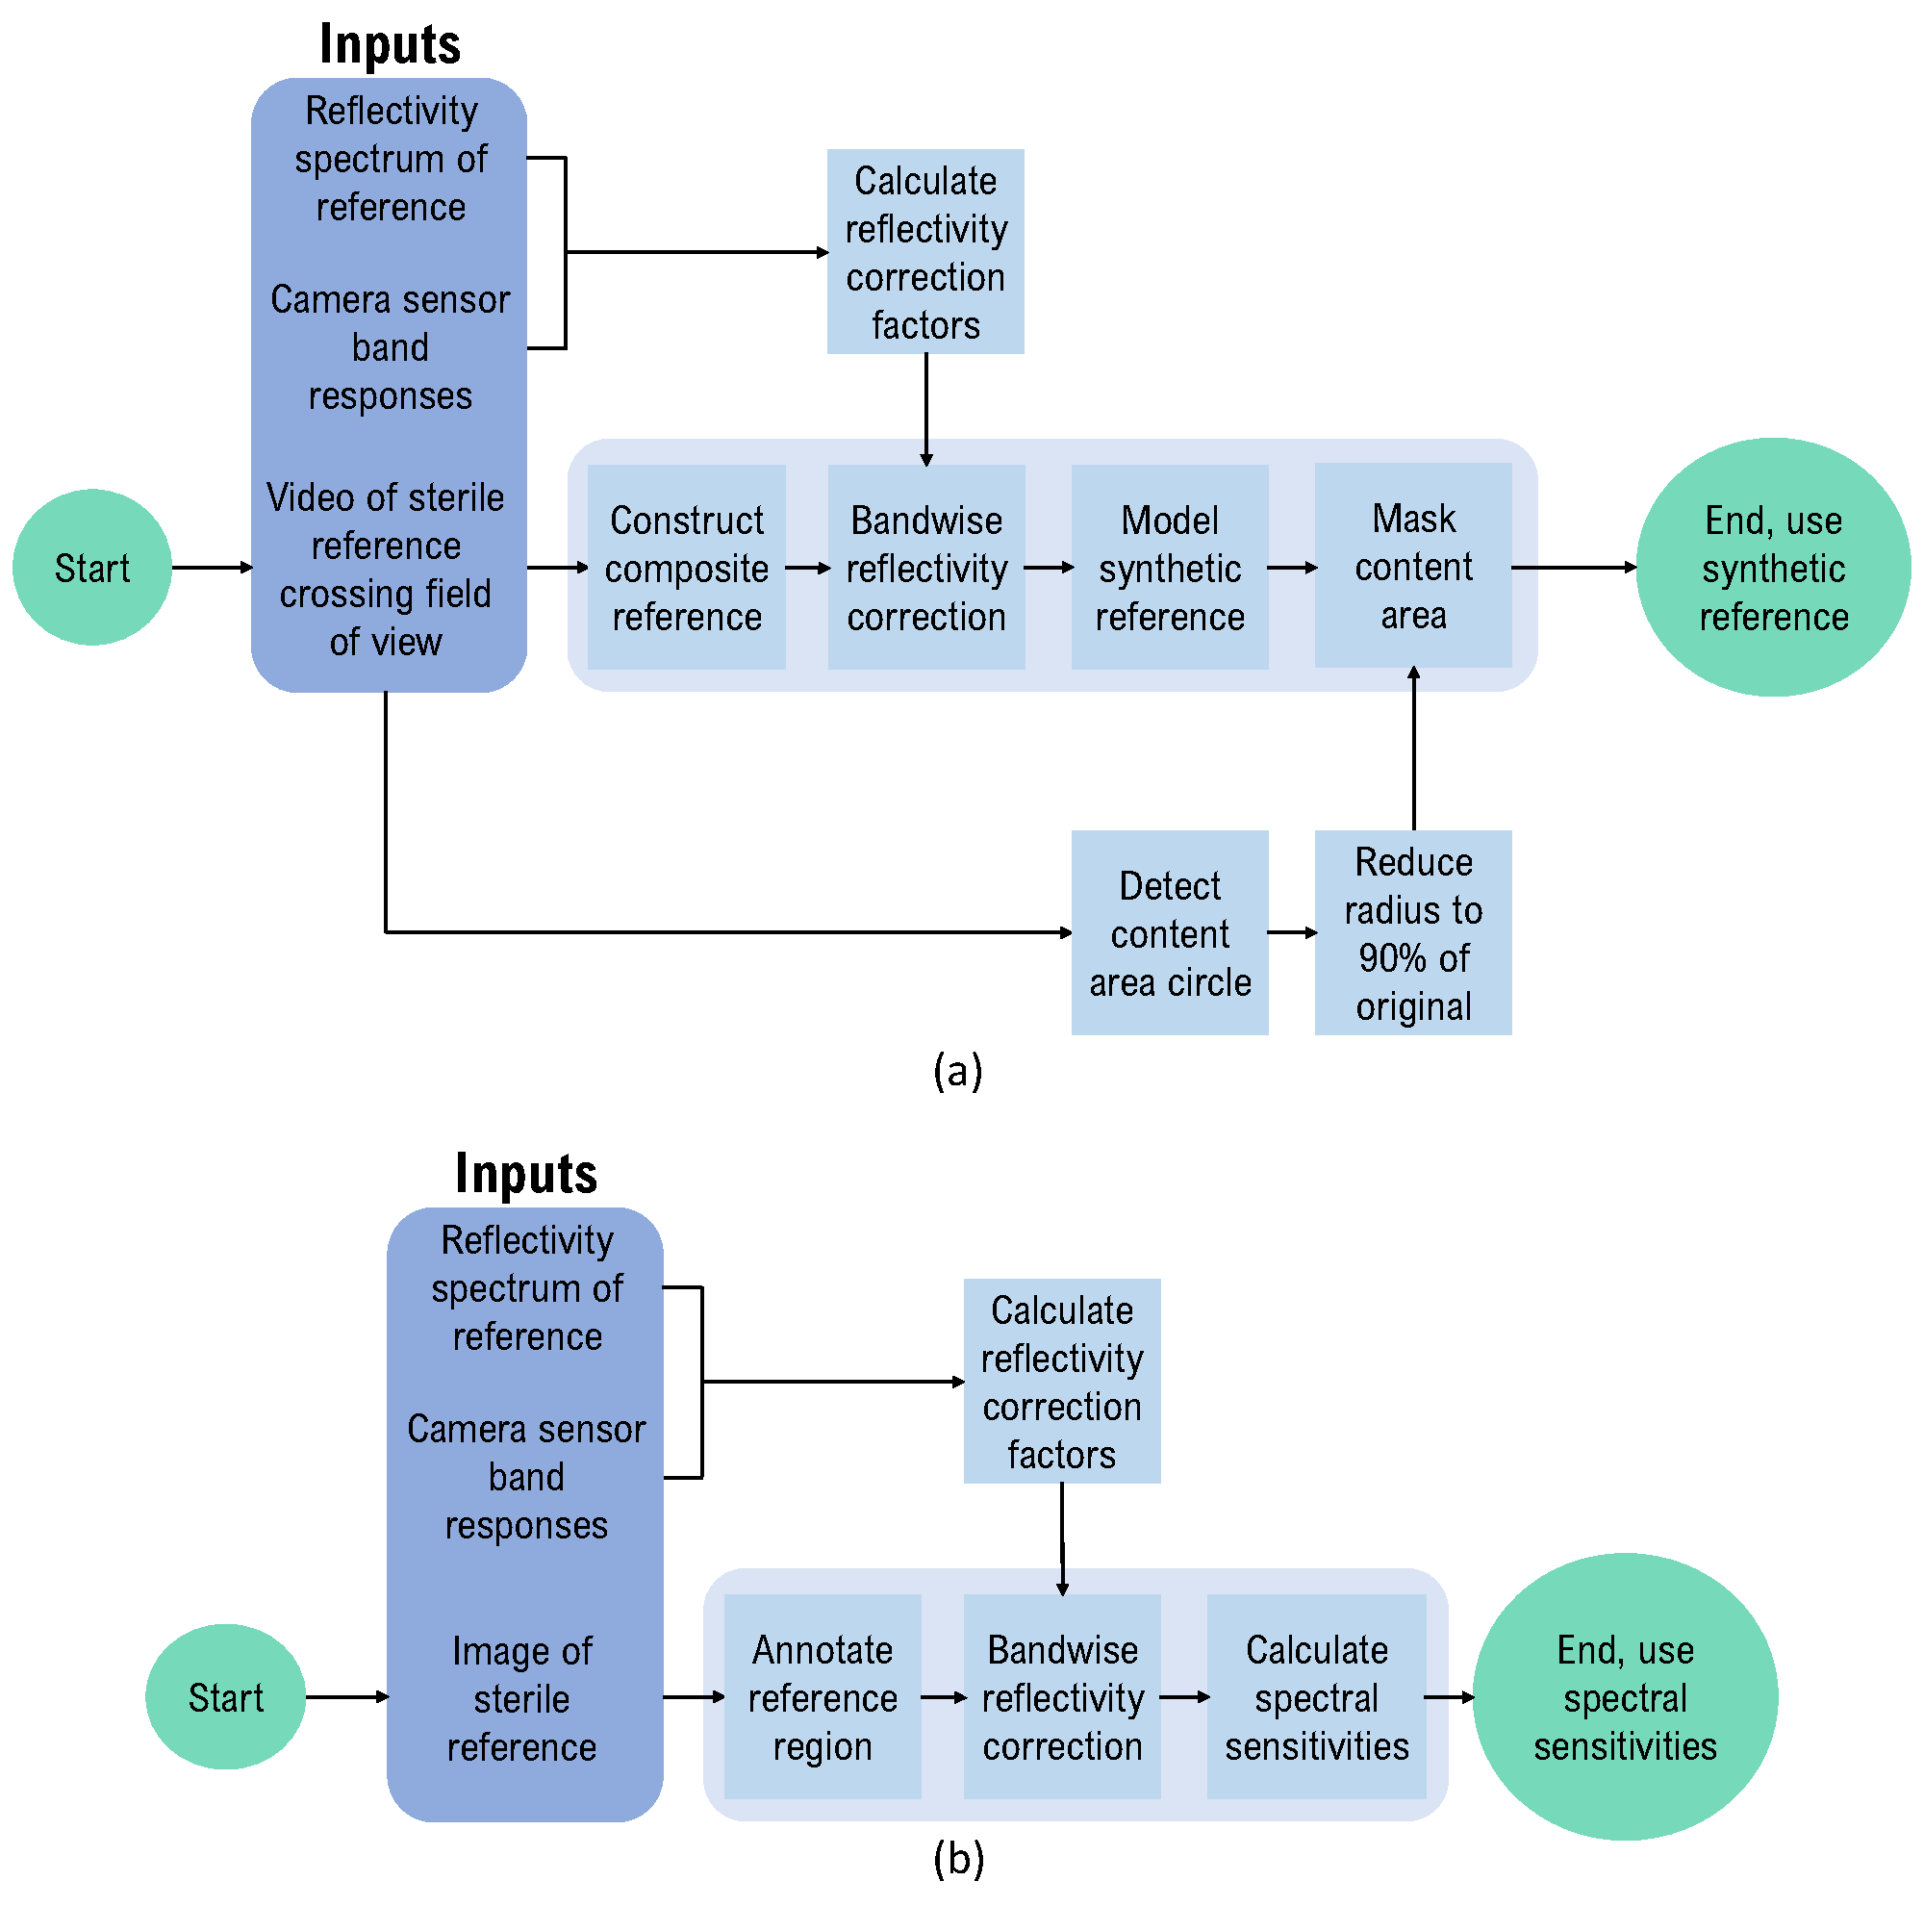
\includegraphics[width=\textwidth]{Figure2}
	% \end{subfigure}
 \caption{Flow charts demonstrating the algorithms for using a sterile reference to white balance intra-operative data for quantitative (a) or relative (b) spectral reconstructions.}
 \label{fig:algorithm}
\end{figure}

%\FloatBarrier
\subsubsection{Generating composite image}
\label{algorithmcomposite}
Hyperspectral videos capture information across space, wavelength and time.
%
The video frames are stacked to create a spatio-spectral $x,y$ plane due to the mosaic structure, and a temporal $z$ axis.
%
%
%
%
Because of the sweeping motion of the bright ruler,
for each spatio-spectral pixel in the $x, y$ plane there is a temporal distribution of measured intensities, which alternates between background and sterile reference intensities in the $z$ axis.
The temporal regions corresponding to the sterile reference are isolated, as detailed below, and the median of these chosen as the value for that spatio-spectral location in the composite reference.
To segment these temporal regions,
%
%
%
we first pre-process the per pixel temporal intensity profile to suppress the impact of background values to a large extent by setting to 0 all the values whose intensity lie below a threshold computed with a classical parameter-free Otsu's method~\citep{Otsu1979} (using skimage v0.19.2 \href{https://scikit-image.org/docs/stable/api/skimage.filters.html\#skimage.filters.threshold_otsu}{\texttt{skimage.filters.threshold\_otsu}} function.)
We further clamp high intensities close to saturation with a fixed threshold in order to remove the impact of specular reflections.
%
These pre-processed temporal profiles are then smoothed using a Savitsky-Golay filter, with window size 15 and order 2
%
~\citep{Savitzky1964a}
(using SciPy v1.8.1 \href{https://docs.scipy.org/doc/scipy/reference/generated/scipy.signal.savgol_filter.html}{\texttt{scipy.signal.savgol\_filter}} function),
%
to limit the impact of noise.
Temporal gradients are then calculated for the resulting pre-processed intensities.
Finally, the peaks, detected using a peak picking algorithm which finds all local maxima by simple comparison of neighboring values and refines these based on their height and prominence (using SciPy v1.8.1 \href{https://docs.scipy.org/doc/scipy/reference/generated/scipy.signal.find_peaks.html}{\texttt{scipy.signal.find\_peaks}} function),
%
are used to identify the temporal regions of interest.
The median of the raw values in these regions, prior to smoothing and thresholding, is then recorded and used as the estimated intensity of that spatial location in the initial mosaic composite reference $W^{c,m}(x, y)$.
% 
% 
% 
% 	
% 	
% 	
% 	
% 
% 

%\FloatBarrier
\subsubsection{A priori ruler reflectivity correction}
\label{algorithmreflectivity}
The sterile ruler was measured in the laboratory using a benchtop spectrophotometer to obtain its reflectance spectrum $t(\lambda)$ as seen in \figref{fig:rulerspectrum}.
%
%
This ruler back can be approximated as a Lambertian surface as variation in spectrum due to small angle changes is small, and the images of this ruler appear matte with few specular reflections. The ideal imaging condition is fronto-parallel imaging, so angle deviations from this are considered sufficiently small as to have negligible effect. 
%
%
From there,
an a priori reflectivity correction factor $\rho^{a}_{n}$ is calculated per band $n$ of the mosaic sensor:
\begin{linenomath*}
\begin{equation}
	\rho^{a}_{n} = \frac{\int t(\lambda)b_n(\lambda) d\lambda}{\int b_n(\lambda) d\lambda}
\label{eq:reflectivitycorrection}
\end{equation}
\end{linenomath*}
where $b_n(\lambda)$ is the band response as provided by the sensor manufacturer. Both the reflectivity correction factors and the band responses can be seen in \figref{fig:rulerspectrum}. %
\begin{figure}[h!]
	\centering
	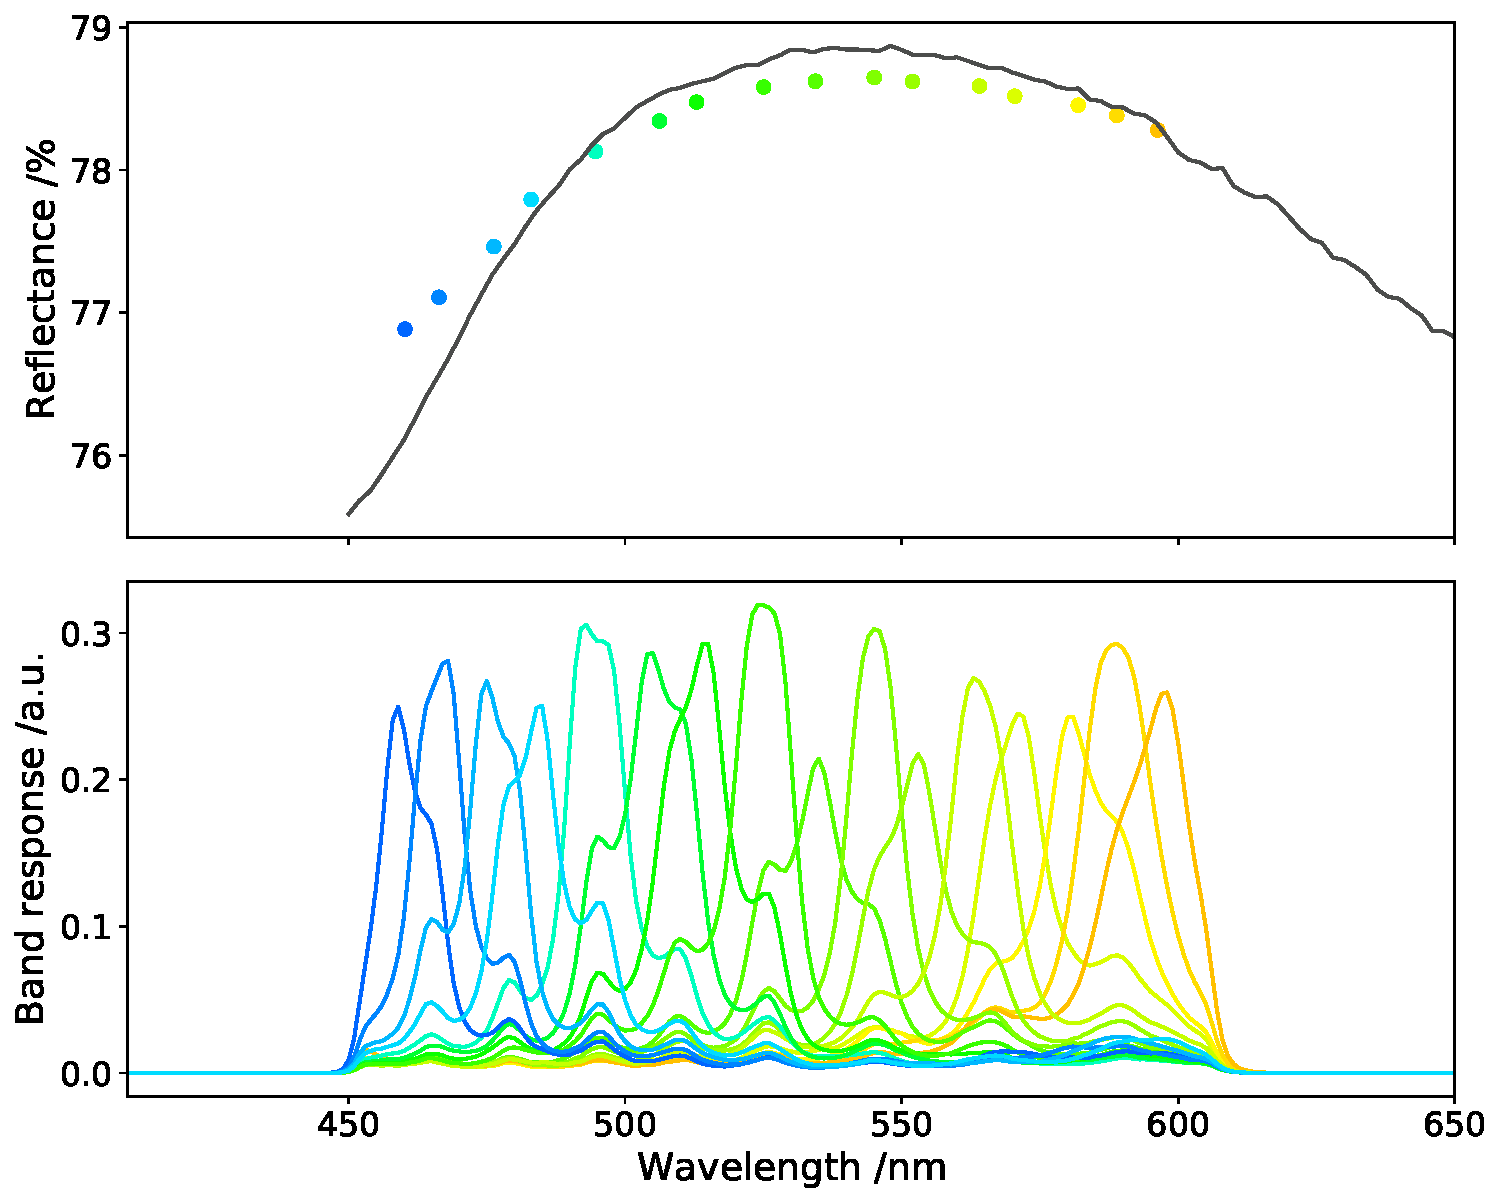
\includegraphics[width=0.9\textwidth]{Figure3.pdf}
	\caption{The reflectance spectrum of the ruler surface without markings and the appropriate reflectivity correction factors computed from this (top) and the band responses of the camera (bottom).}
	\label{fig:rulerspectrum}
\end{figure}

Each pixel of the initial composite reference $W^{\textrm{ic}}(i,j,n)$ is then divided by the a priori correction factor $\rho^{a}_{n}$ for the appropriate band to form the final composite reference: $W^{\textrm{c}}(i,j,n) = W^{\textrm{ic}}(i,j,n)/\rho^{a}_{n}$.
%
We note that this correction captures the sensor band responses and the spectrum of the ruler as known a priori but does not account for the unknown spectrum of the light source used intraoperatively. This provides an essential step in the generation of synthetic references or the spectral sensitivities. 
%
In the generation of synthetic references, this correction is performed on a composite reference which may also present important imperfections due to noise and video input processing. We aim to mitigate these through our separable model fitting.
%
%



 

%\FloatBarrier
\subsubsection{Separable model parameter fitting}
\label{algorithmparameters}
A variety of methods can be used to calculate the factors in \eqref{eq:modelling white references}. We present three options which vary in their modelling of the vignetting, and whether the spectral sensitivities and scalar factor are fitted jointly or sequentially. For simplicity, we present the methods given a measured white reference $W(i,j,n)$ as input although they can also be applied to a composite white reference $W^{\textrm{c}}(i,j,n)$.

\paragraph{Vignetting modelled non-parametrically}
The first method only makes use of the separability assumption, models the vignetting as a non-parametric function, and calculates the spectral sensitivities and scalar factor. Since vignetting is modelled as independent of wavelength, it should be identical for all bands.
Making use of our convention that $\frac{1}{N} \sum_{n}S(n) = 1$, and assuming a zero mean noise pattern $N(i,j,n)$, we find that, up to residual noise, \eqref{eq:modelling white references} leads to:
%
%
\begin{linenomath*}
\begin{equation}
	M V(i,j) \approx \frac{1}{N}\sum_{n} W(i,j,n)
\label{eq:nonpara1}
\end{equation} 
\end{linenomath*}
%
Making use of our second convention that $\max_{i,j}V(i,j) = 1$, we find that, up to residual noise:
\begin{align}
	M &\approx \max_{i,j}\left( \frac{1}{N}\sum_{n} W(i,j,n) \right) \\
	V(i,j) &\approx \frac{ \frac{1}{N}\sum_{n} W(i,j,n) }{ \max_{i,j}\left( \frac{1}{N}\sum_{n} W(i,j,n) \right) }
\end{align} 
%
Finally, spectral sensitivities can be estimated by:
%
%
%	
%
%
\begin{linenomath*}
\begin{equation}
	S(n) \approx \frac{\sum_{i,j}W(i,j,n)}{\frac{1}{N}\sum_{i,j,n'}W(i,j,n')}
\label{eq:nonpara2}
\end{equation}
\end{linenomath*}
%
This method accounts for imperfections in the system such as dust on lenses more appropriately, however it is also more likely to retain imperfections from the input reference, for example artefacts in the compositing process. It is this \eqref{eq:nonpara2} that is used to calculate the spectral sensitivities for balancing of relative data as in \figref{fig:algorithm}b.

\paragraph{Vignetting modelled with a Gaussian function}
Alternatively, a parametric model can be used to capture the vignetting.
As is standard in computer vision, we use a two-dimensional, normalized, isotropic Gaussian for this purpose:
\begin{linenomath*}
\begin{equation}
	V(i,j) = \exp\left(-\frac{(i-\mu_i)^2}{2\sigma^2} - \frac{(j-\mu_j)^2}{2\sigma^2} \right)
\label{eq:2DGauss}
\end{equation}
\end{linenomath*}
%
where $\mu_i$ and $\mu_j$ represent the co-ordinates of the centre of the Gaussian in the $i$ and $j$ directions respectively and $\sigma$ represents the standard deviation. 
%

Our second method fits the Gaussian parameters, the scalar factor and spectral sensitivities using a joint least squares approach:
%
\begin{linenomath*}
\begin{equation}
	\argmin_{\mu_i,\mu_j,\sigma, M, \{S(n)\}_{n}} \sum || W(i,j,n) - MS(n) \exp\big( -\frac{(i-\mu_i)^2}{2\sigma^2} - \frac{(j-\mu_j)^2}{2\sigma^2}\big) ||^2
\end{equation}
\end{linenomath*}

The third method calculates the scalar factor $M^{\textrm{est}}$ and spectral sensitivities $S^{\textrm{est}}(n)$ as in the first method with the Gaussian fitted to the non-parametric vignetting using a 
%
least squares approach on the Gaussian parameters only:
\begin{linenomath*}
\begin{equation}
	\argmin_{\mu_i,\mu_j,\sigma} \sum || W(i,j,n) - M^{\textrm{est}}S^{\textrm{est}}(n) \exp\big( -\frac{(i-\mu_i)^2}{2\sigma^2} - \frac{(j-\mu_j)^2}{2\sigma^2}\big) ||^2
\end{equation}
\end{linenomath*}
%
%
As will be apparent from our experiments, this third method provides advantageous benefits due to the Gaussian fit mitigating imperfections in the composite reference, whilst minimising the computational time.

%
%

\paragraph{Masking content area}
Finally, as detailed in \citet{Munzer2013,Huber2022}, imaging through a scope leads to a circular content area which needs to be taken in to account in our computational pipeline.
In this work, the content area disk
%
is detected from a frame of a video using a pre-trained neural network~\citep{Huber2022} (using the implementation at \url{https://github.com/RViMLab/endoscopy}.)
The radius is reduced to 90\% of its original size to discount edge effects. This circle is then used to mask the content area as the final step to generate the synthetic white reference.

% 
% 
%     
%    
%     
%     

% 
%    
%    
%    
%    
%     
%   

% 
%  
%     
%     
%    
% 
%    
%    
%  
%     
%     
%     

% 
%                       
% 
% 

%

%\FloatBarrier
\subsubsection{Balancing using only spectral sensitivity for relative data}
\label{algorithmrelative}
For some use cases, absolute reflectance information $R(i,j,n)$ is not required so relative data is sufficient as described in \secref{intro}.
When normalising the spectral data at each pixel after \eqref{eq:WBfull} using \newline $R^{\textrm{norm}}(i,j,n) = R(i,j,n) / \frac{1}{N}\sum_{n'}|R(i,j,n')|$, the spatial effects of the vignetting $V(i,j)$ and absolute intensity information arising from $M$ is lost.
In this context, only spectral sensitivities are required for white balancing.
Dismissing the effect of dark images for simplicity, this is performed as follows:
\begin{linenomath*}
\begin{equation}
    R^{\textrm{norm}}(i,j,n) \approx \frac{I(i,j,n)}{S(n) \frac{1}{N}\sum_{n'}|\frac{I(i,j,n')}{S(n')}|} 
\end{equation}
\end{linenomath*}
However this removes the possibility of proper sRGB or CIELAB construction.
%
%
%
%
The simplified algorithm using only a single image of the ruler to generate these spectral sensitivities is also depicted in \figref{fig:algorithm}b. 

%\FloatBarrier
\subsection{Evaluation methodology for synthetic references}
\label{methodsynthetic}
For each distance in our experimental setup, a video of the ruler moving across the field of view was taken against a static background.
These were used to construct synthetic white references for each distance using the model described in \secref{methodmodel} with Gaussian vignetting and calculated scalar factor and spectral sensitivities.
%
Synthetic references were then used to reconstruct quantitative spectra from our checkerboard datasets and the errors calculated as in 
%
\secref{methodmotivation}.

The similarity of the synthetic references to measured references was evaluated using a range of metrics.
The pixel-by-pixel absolute percentage errors between the synthetic and measured references, and the absolute percentage errors between each set of spectral sensitivities were summarized in terms of median absolute percentage error ($\MedAPE$):
% 
%
\begin{linenomath*}
\begin{equation}
    \MedAPE\big(u(\cdot),u^{\textrm{ref}}(\cdot)\big) = \median_{k}\Big|\frac{u(k) - u^{\textrm{ref}}(k)}{u^{\textrm{ref}}(k)}\Big|
\label{eq:abspercenterr}
\end{equation}
\end{linenomath*}
where $u$ is a given signal compared against a given reference $u^{\textrm{ref}}$ both indexed by $k$.


For the evaluation of the relative spectra achieved with the method presented in \secref{algorithmrelative},
a single set of spectral sensitivities is calculated based on the lighting conditions from a 150 pixel radius region of interest in a single image of a ruler.
%
These spectral sensitivities are then used to reconstruct the relative spectra at all distances and the errors calculated in these as in \secref{methodmotivation}.
However, good sRGB and CIELAB reconstructions cannot be computed from relative data as the intensity information is lost so this analysis is not performed in this case.

Finally, the synthetic reference method is evaluated in terms of surgical workflow integration in a sterile environment by its use in a human cadaveric spine surgery. Qualitative evaluation is performed on sRGB reconstructions as part of \secref{resultsintegration}.
%

%\FloatBarrier
\section{Results}
\label{results}
\subsection{Impact of improper white balancing}%
\label{resultsnecessity}
Datasets were obtained at a variety of distances and under different lighting conditions as described in \secref{methodmotivation}. 
% 
%
To summarize this spectral data, six representative tiles of interest (A1, C3, D4, F1, F3, F4) are displayed for the variety of white balancing regimes investigated in \figref{fig:summaryspectranecessity}, and the sRGB reconstructions of each regime for the dataset at 20 cm shown in \figref{fig:summarysRGBnecessity}. These tiles demonstrate primary colors and some colors expected in surgical scenes. The associated errors for these data are shown in \tabref{tb:badwhites}. 

The first regime shows the optimally reconstructed spectra for a variety of distances of the camera from the checkerboard. These are calculated by balancing each dataset obtained using the Karl Storz D light C using a measured Spectralon white reference obtained at the same location as the data with the same light source, which is not possible in a surgical environment.

To demonstrate the impact of the white reference being obtained at a different distance to the subject, the checkerboard data at all distances is balanced with the white reference obtained at 35 cm. Visually a wider spread of intensities in quantitative spectra can be seen, and the errors confirm that as the distance varies from that of the white reference the errors in the quantitative reconstructed spectra also increase, as seen in \figref{fig:summaryspectranecessity}. The $\Delta E$ values and sRGB reconstructions do not show a significant difference compared to the correctly balanced spectra as a large amount of spectral information is lost on conversion to sRGB or CIELAB which reflects the increase in information expected from the use of hyperspectral imaging compared to conventional cameras. 

Another likely problem with limited white referencing in a surgical setting is the likelihood of changing lighting conditions. This was mimicked by obtaining a white reference with the Karl Storz LED light source at each distance and using this to balance the data collected with a different light source, the Karl Storz D light C, which was then processed as above. The resulting errors, spectra, and sRGB reconstructions clearly show the importance of white referencing to account for the lighting conditions of the scene as the shape of the spectra are significantly changed in both quantitative and relative spectra which is also clearly visible in the sRGB reconstruction and all error metrics so any change in lighting must be accounted for. 
\begin{figure}[hp!]
	\centering
        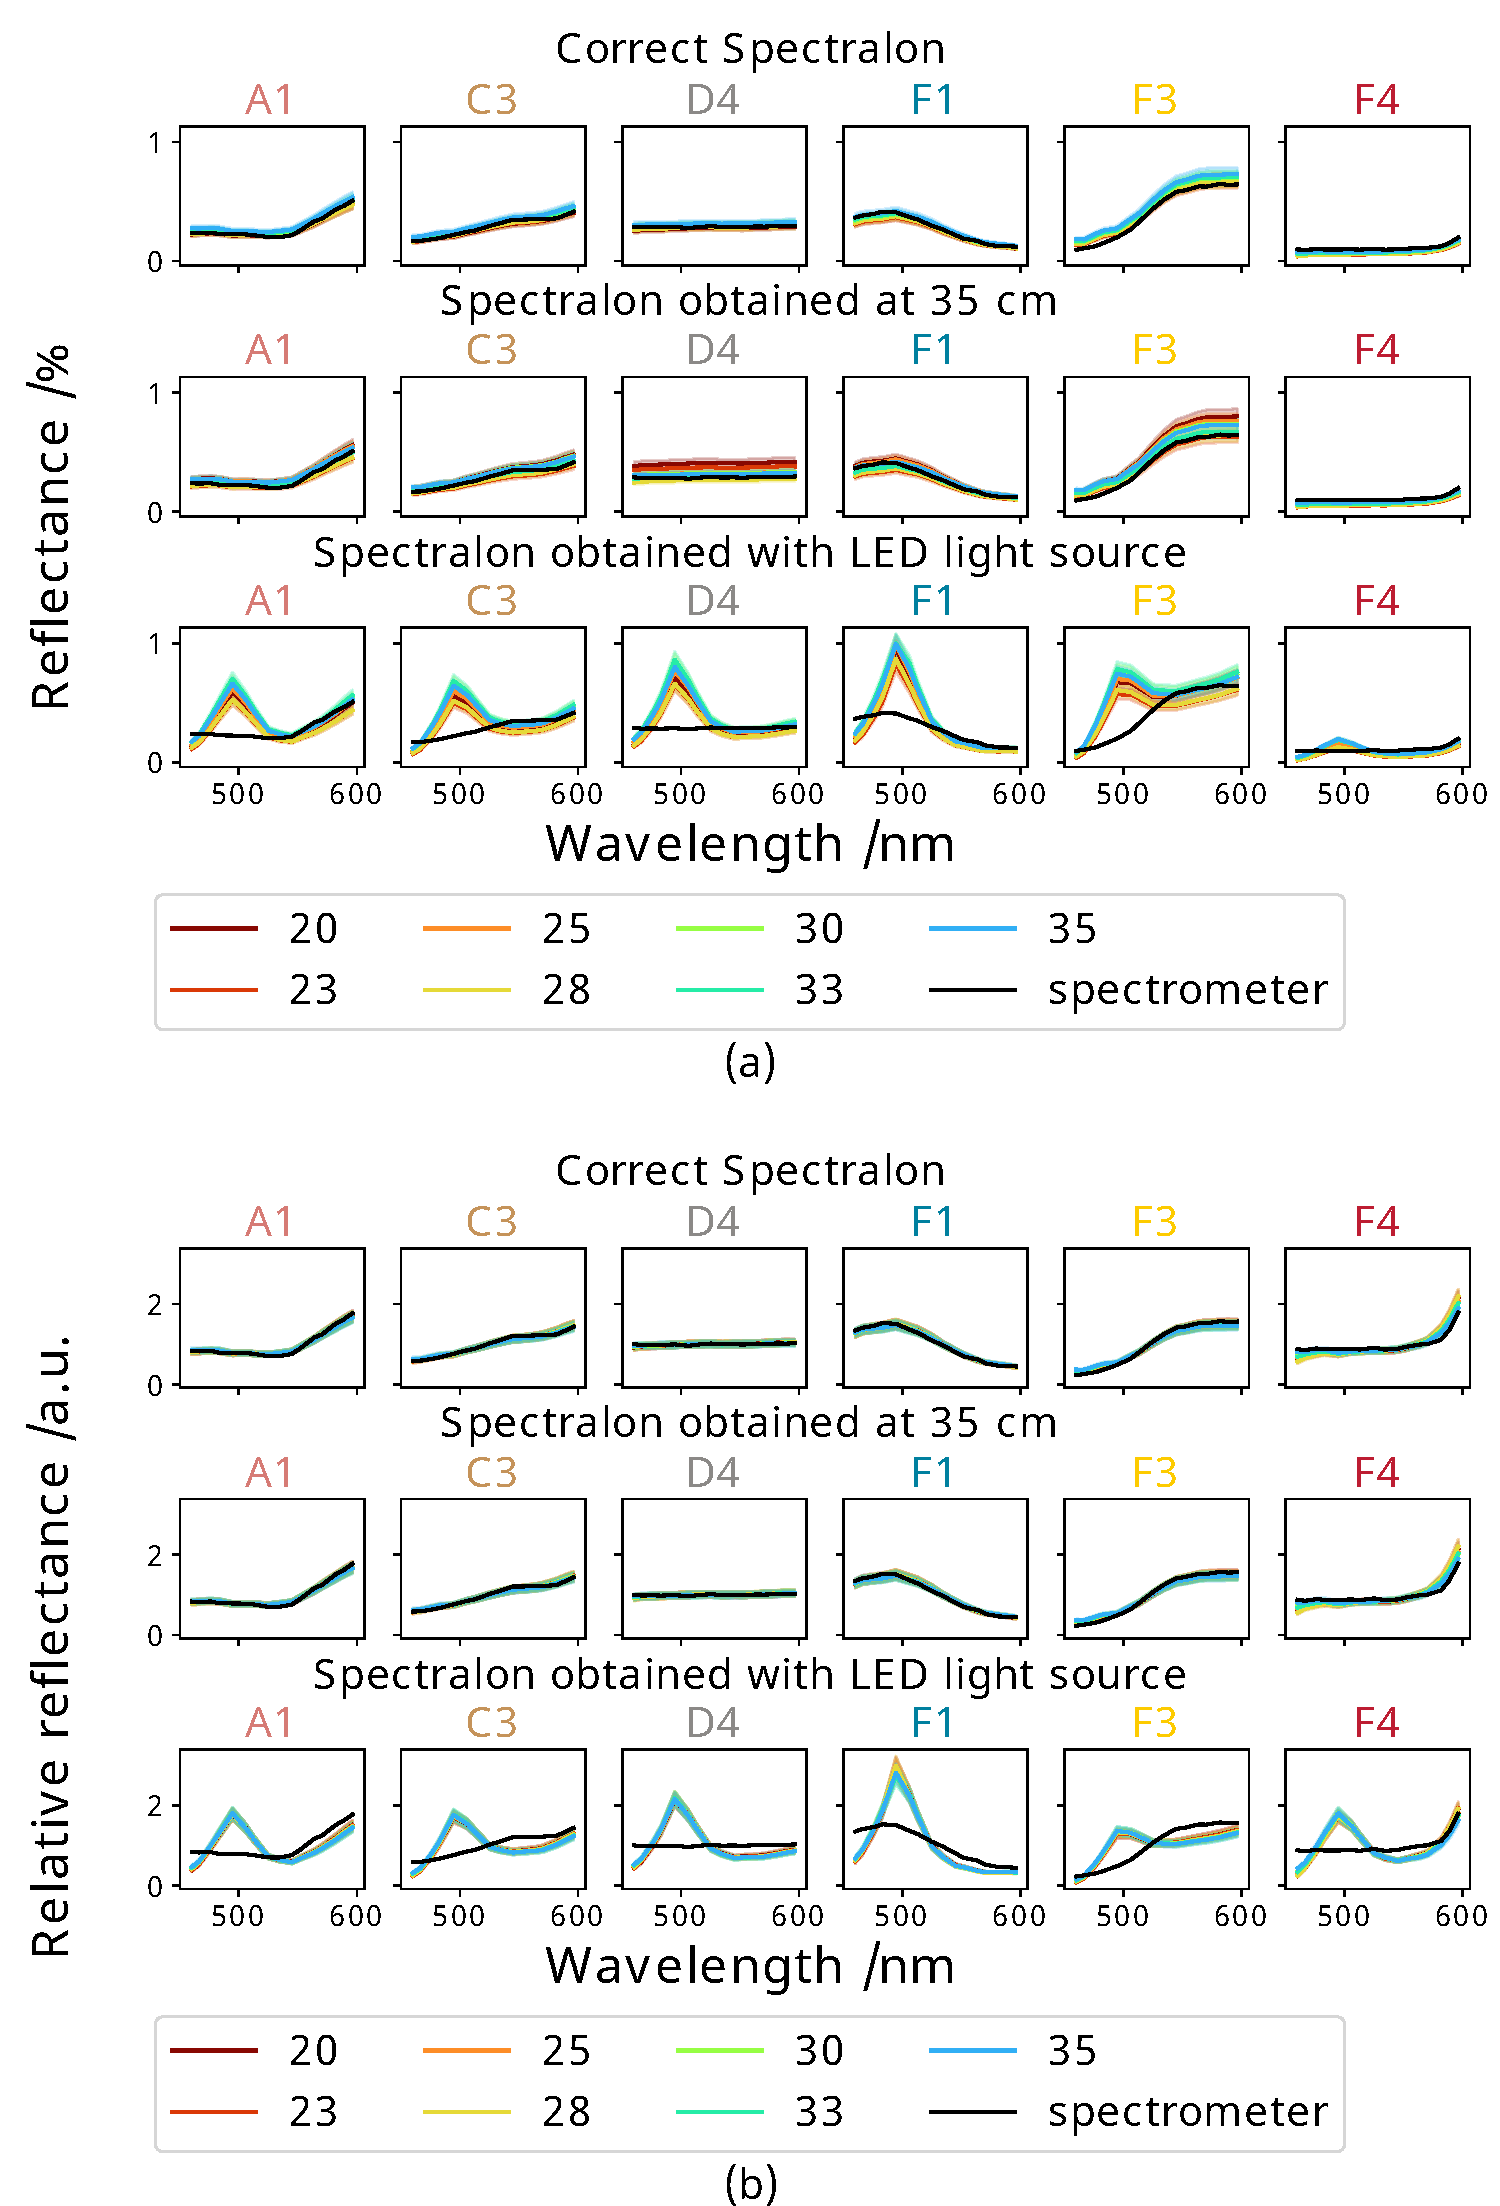
\includegraphics[width=0.9\textwidth]{Figure4}
	% \begin{subfigure}[htp!]{0.79\textwidth}
	%     \includegraphics[width=\textwidth]{Figure4a}
	%     \caption{}
	%     \label{fig:BadWhitesSpectra}
	% \end{subfigure}
 %        \begin{subfigure}[htp!]{0.79\textwidth}
	%     \includegraphics[width=\textwidth]{Figure4b}
	%     \caption{}
	%     \label{fig:BadWhitesSpectraNorm}
	% \end{subfigure}
 \caption{The mean spectrum of a selection of tiles as measured from each distance (cm) plotted against the spectrometer measurement of that tile, where each plot represents a new tile (labelled above it as corresponding to those in \figref{fig:setup}b) for both (a) quantitative and (b) relative data. At each distance the data is balanced with either the correct Spectralon white reference image, the Spectralon reference obtained at 35cm, or the Spectralon reference obtained using a different light source.}
 \label{fig:summaryspectranecessity}
\end{figure}
\begin{figure}[t!]
    % \ContinuedFloat
    \centering
        % \begin{subfigure}[htp!]{0.55\textwidth}
    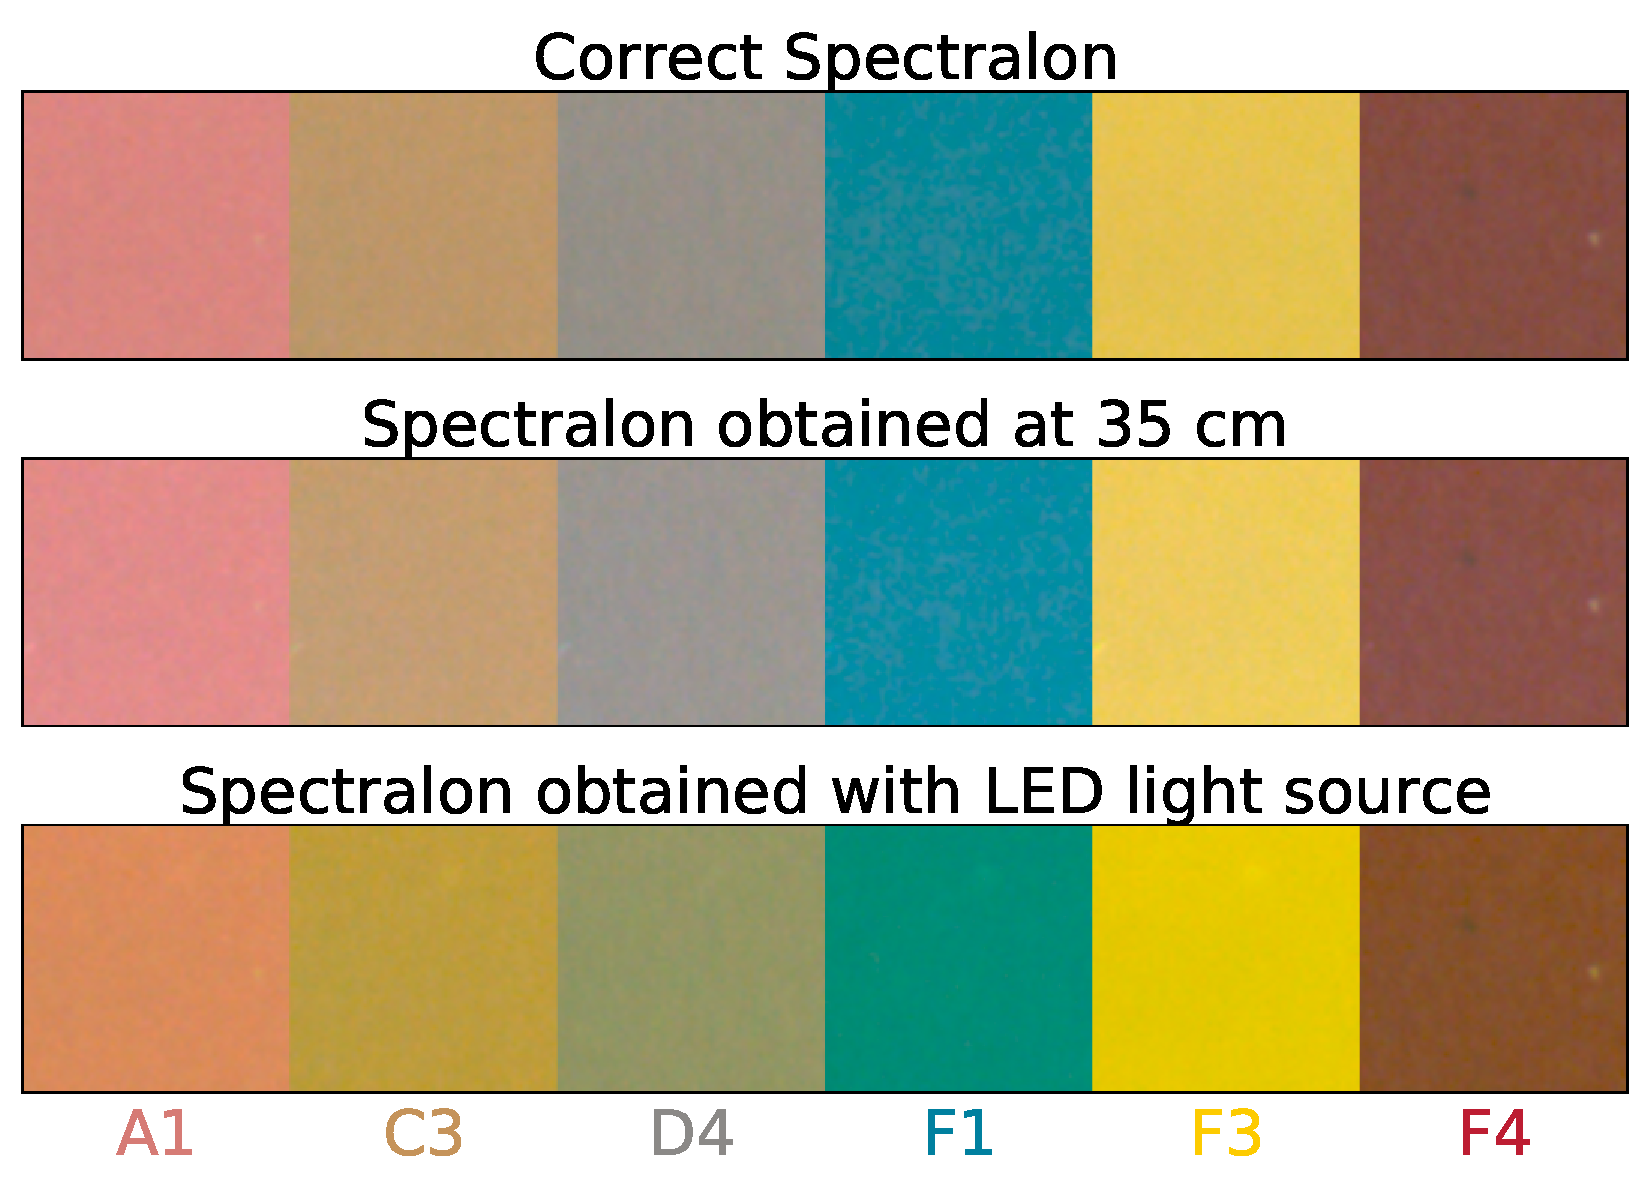
\includegraphics[width=0.7\textwidth]{Figure5}
	% \end{subfigure}
    \caption{sRGB reconstructions of the central 200 x 200 pixels of a selection of tiles (labelled below as corresponding to those in \figref{fig:setup}b) taken at 20 cm and balanced with either the correct Spectralon white reference image, the Spectralon reference obtained at 35cm, or the Spectralon reference obtained using a different light source.}
    \label{fig:summarysRGBnecessity}
\end{figure}
\begin{table}[tbph]
    \caption{The mean $\NRMSE$ for the mean measured spectrum of each tile compared to its spectrometer spectrum of each quantitative and relative dataset, alongside the median pixel-by-pixel $\Delta E$ value between the composite CIELAB reconstructions compared to the literature values. These datasets are balanced with the correct Spectralon reference, the Spectralon reference obtained at 35cm, or the Spectralon reference obtained using an LED light source.}
    \csvloop{
file = BadWhites.csv, 
head to column names,
before reading = \centering\sisetup{round-mode=figures, round-precision=3},
tabular={|l|SSS|SSS|SSS|@{}c},
table head = \hline 
& \multicolumn{3}{c}{\textbf{$\NRMSE$ for Quantitative}} & \multicolumn{3}{|c|}{\textbf{$\Delta E$}} & \multicolumn{3}{c|}{\textbf{$\NRMSE$ for Relative}} \\
 & \multicolumn{3}{c}{\textbf{spectra (\%)}} & \multicolumn{3}{|c|}{ } & \multicolumn{3}{c|}{\textbf{spectra (a.u.)}} \\
\rot{\textbf{Distance (cm)}} & \rot{\textbf{Correct Spectralon}} & \rot{\textbf{Spectralon at 35 cm}} & \rot{\textbf{Spectralon using LED}} & \rot{\textbf{Correct Spectralon}} & \rot{\textbf{Spectralon at 35 cm}} & \rot{\textbf{Spectralon using LED}} & \rot{\textbf{Correct Spectralon}} & \rot{\textbf{Spectralon at 35 cm}} & \rot{\textbf{Spectralon using LED}} \\ 
\hline, 
command = \Distance & \qNRMSECorrect & \qNRMSEdist & \qNRMSELED & \qDeltaECorrect & \qDeltaEdist & \qDeltaELED & \nNRMSECorrect & \nNRMSEdist & \nNRMSELED , 
table foot = \hline,
    }
\label{tb:badwhites}
\end{table}

%
% 
% 
% 	
% 	
% 
% 	
% 	
% 	
%   
% 	
% 
% 	
% 	
% 
%
% 
% 	
% 	
% 		
% 		
% 		
% 		
% 		
% 	
% 	
% 		
% 	
% 	
% 	
% 
% 
% 	
% 	
% 	
% 		
% 		
% 		
% 		
% 		
% 	
% 	
% 	 
% 	
% 
% 
% 
%
% 	
% 	
% 	  
% 	
% 	  
% 	
% 
% 	 
% 	    
% 
% 	
%
% 
%     
%     
% 	
% 	 
% 	   
% 	 
% 	
% 	
% 	  
% 	  
% 	
% 	
% 
% 
%
%
% 
% 	
% 	
% 	    
% 	  
% 	    
% 	
	% 
	%    
	%    
	%  
	%
    % 
% 	
% 	   
% 	  
% 	   
% 	
% 
% 
%    
% 	
	% 
	%     
	%    
	%    
	% 
	%
	%    
	%  
	%   
	%
	%
	%   
	%    
	%
 % 
% % 
    % 
	% 
 %
% 	
% 	
%


\FloatBarrier
\subsection{Goodness of fit of the separable white reference models}
\label{resultsmodel}
%
%
The measured white references obtained at each distance were approximated using the non-parametric, Gaussian vignetting with jointly-fitted scalar factor and spectral sensitivities, and Gaussian vignetting with calculated scalar factor and spectral sensitivities methods to determine the inherent errors in using this model and these approximations.
The pixel-by-pixel absolute percentage errors in the resulting approximated references compared to their respective measured references are then plotted in \figref{fig:ModelErrors} and show very low errors across all models.
The models using Gaussian fitting show slightly higher errors, likely due to the inability of the Gaussian fit to account for dust on lenses in the set-up. 

\begin{figure}[h!]
	\centering
	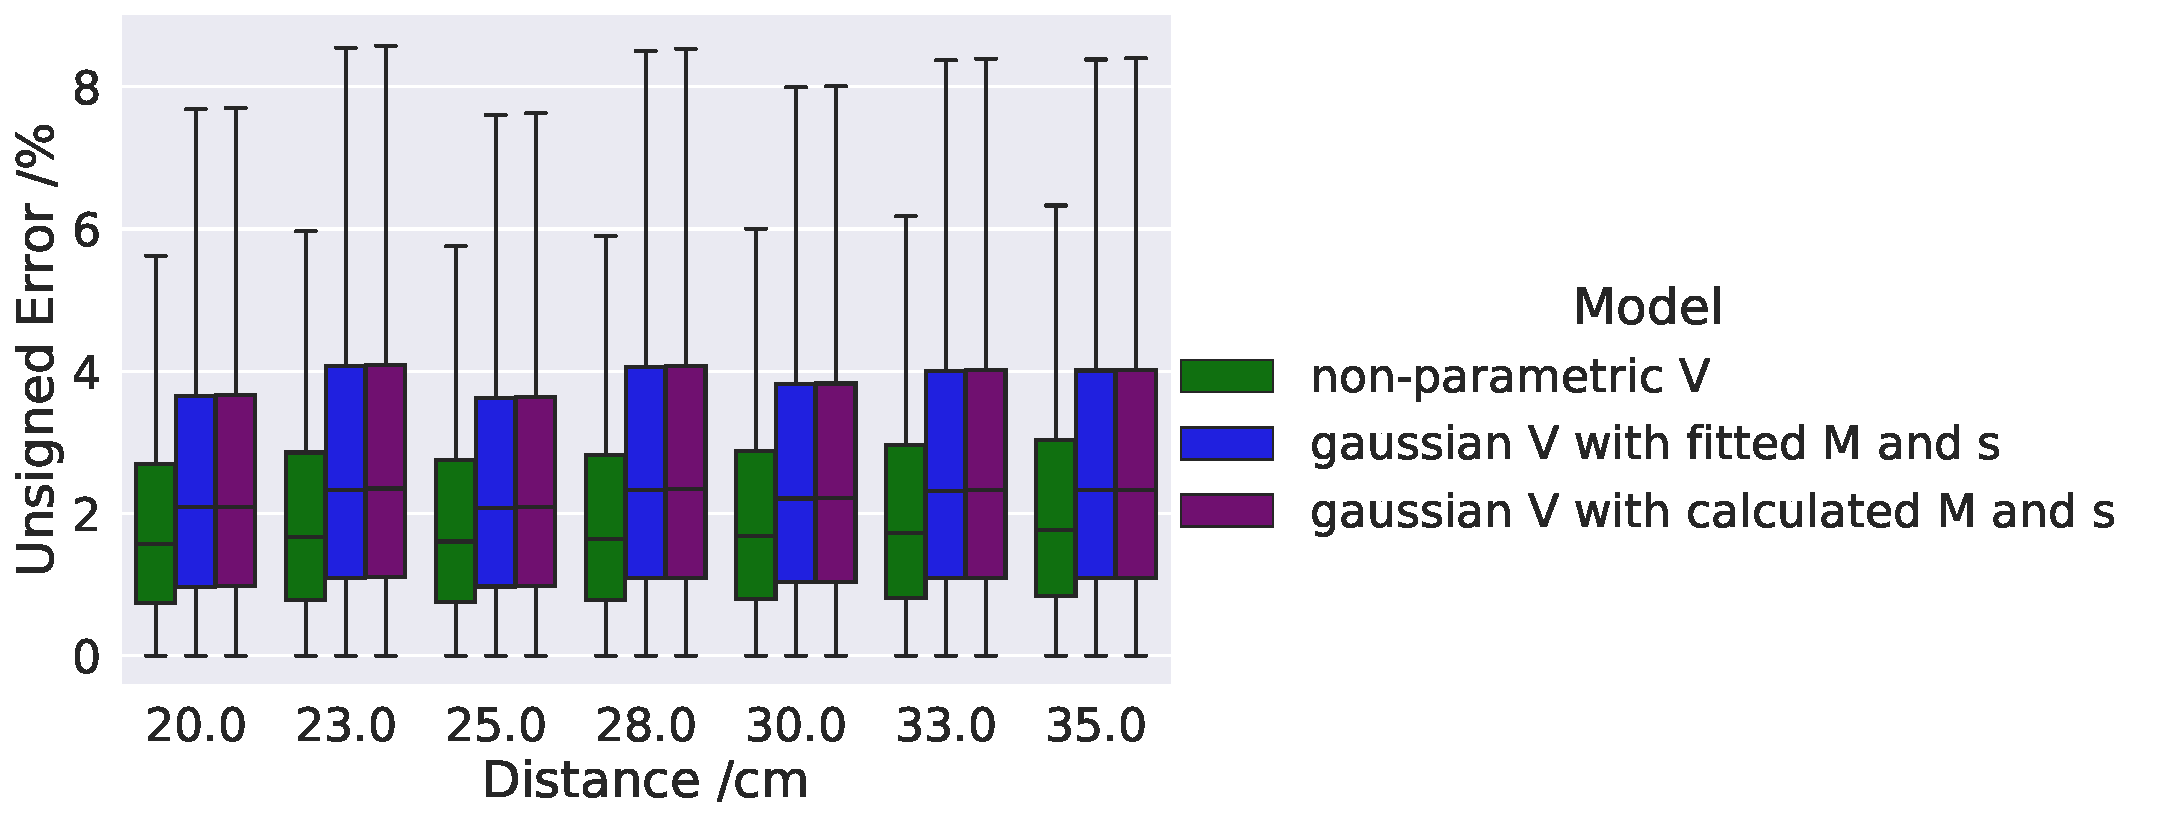
\includegraphics[width=\textwidth]{Figure6}
	\caption{Box plots showing the pixel-by-pixel absolute percentage errors in modelled references compared to the original references at a range of distances using either non-parametric, Gaussian vignetting with fitted scalar factor and spectral sensitivities, and Gaussian vignetting with calculated scalar factor and spectral sensitivities methods.}
	\label{fig:ModelErrors}
\end{figure}

The spectral sensitivities obtained for each model were found to be invariant with respect to distance or approximation method. Any change in distance requires a change in optical focus which results in a change of optical vignetting. This suggests that the spectral sensitivities are unaffected by optical vignetting or its modelling. This lends credence to the assumption that the spatial and spectral dependencies of the components of white references can be separated. 

% 
% 	
% 	
% 	
% 	
% 

This confirms that white reference images can be well modelled using the assumption of separability between spatial and spectral components, and using a two-dimensional isotropic Gaussian.

\FloatBarrier
\subsection{Evaluation of synthetic references from sterile ruler sweeps}
\label{resultssynthetic}
The errors between the synthetic references compared to measured references were calculated as described in \secref{methodsynthetic} and can be seen in \tabref{tb:SynTotErrors} for the synthetic references generated from videos of the ruler against a fixed background obtained at the same position as the data. These show that this method reproduces the measured Spectralon references well, particularly as the errors are comparable to the inherent errors in modelling references shown in \figref{fig:summaryspectrasynthetic}.
\begin{figure}[htp!]
	\centering
        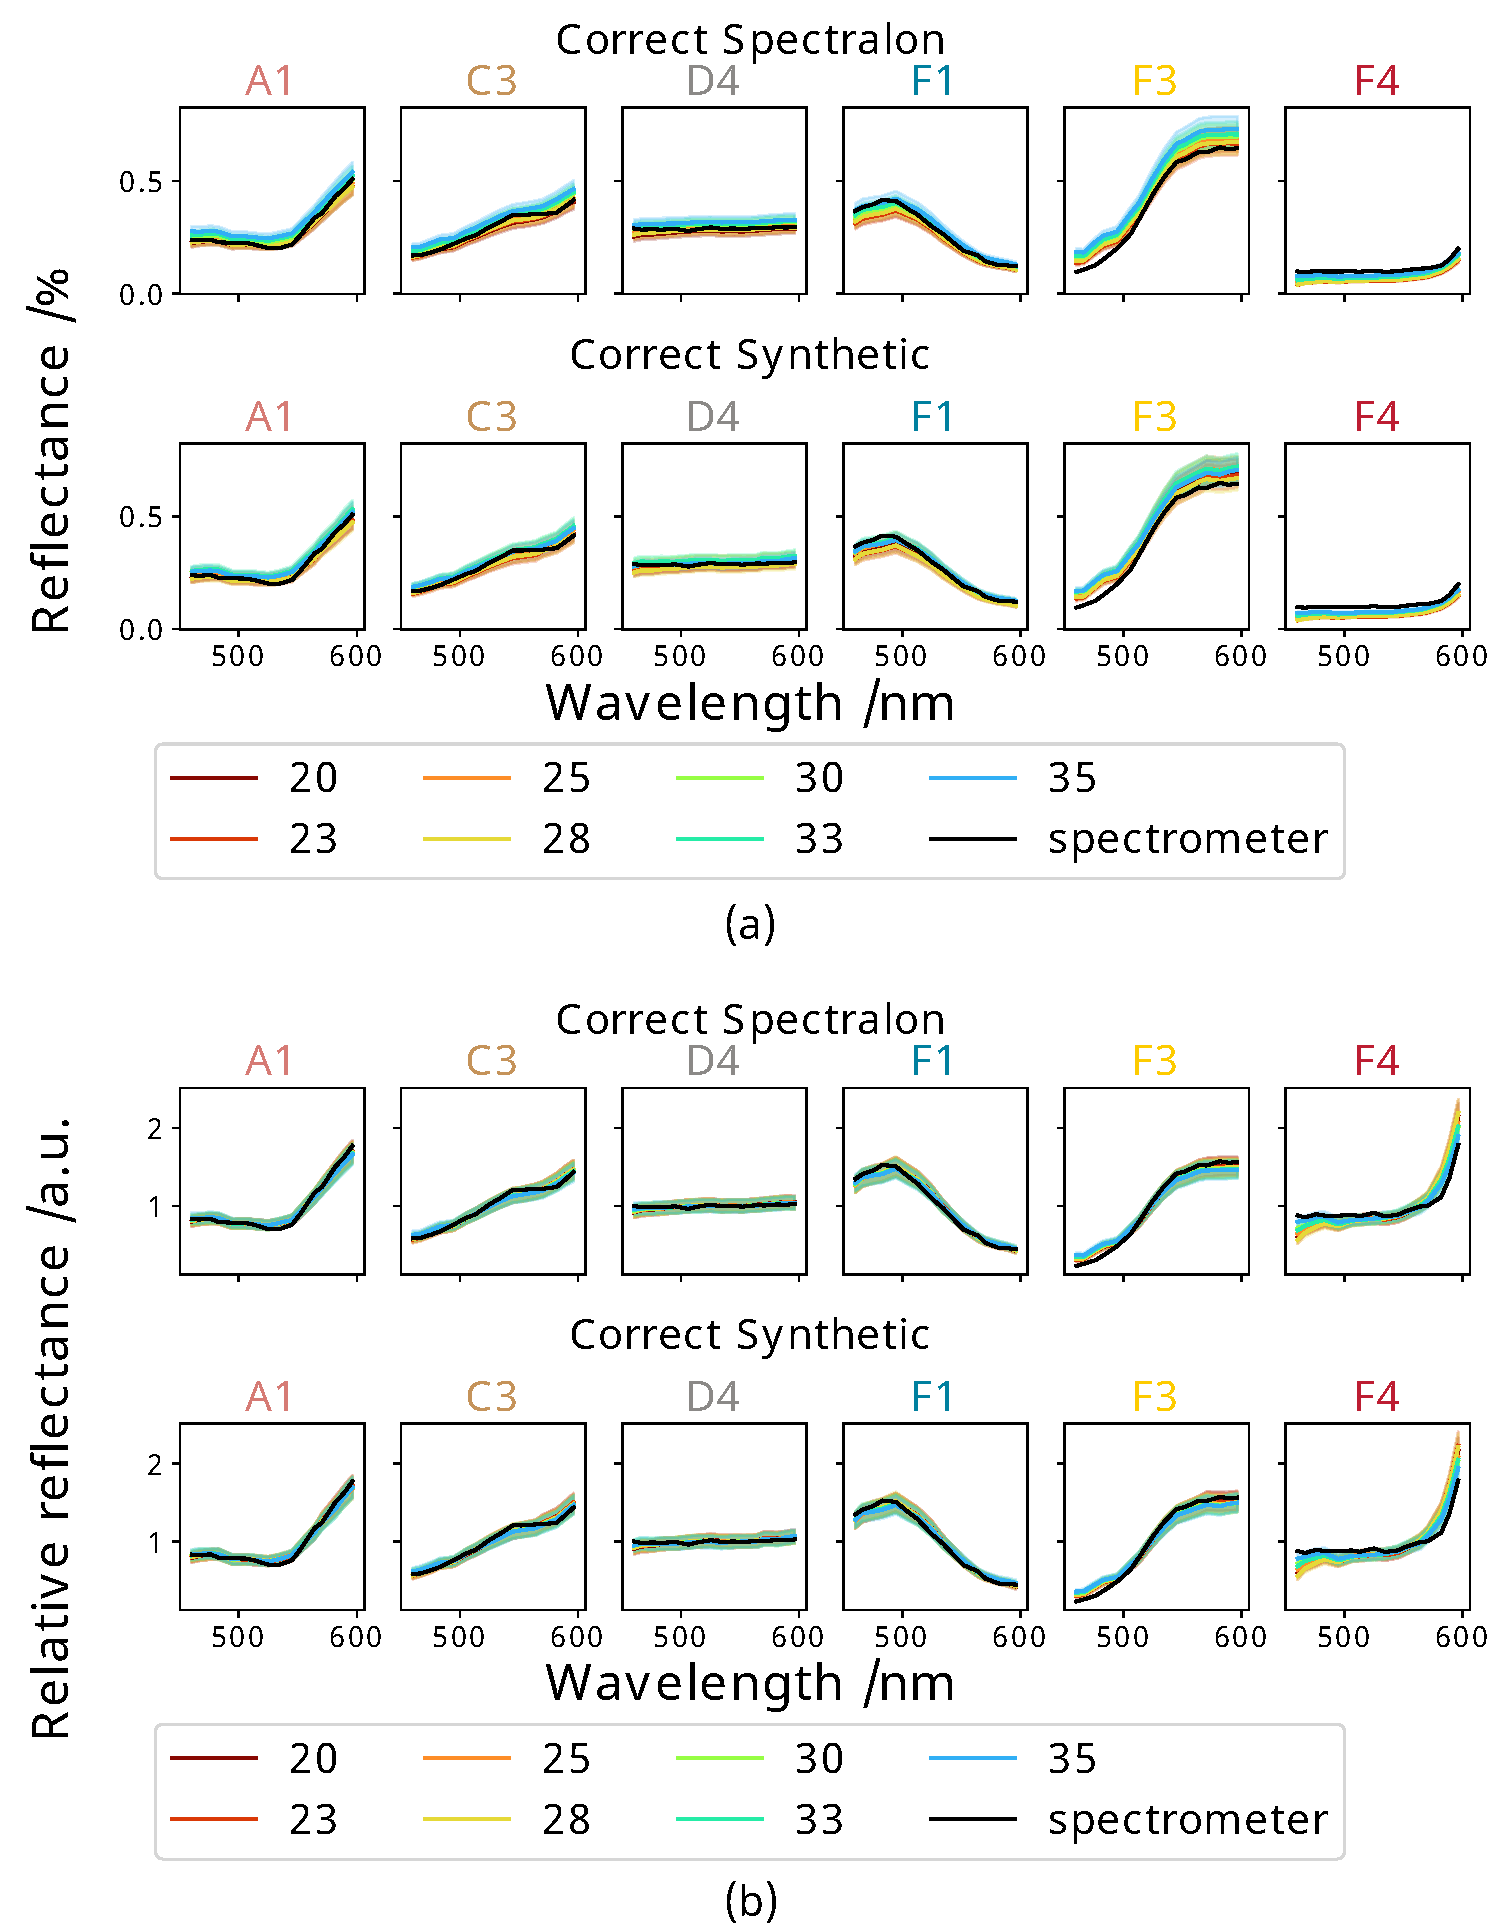
\includegraphics[width=\textwidth]{Figure7}
	% \begin{subfigure}[ht!]{0.79\textwidth}
	%     \includegraphics[width=\textwidth]{Figure7a}
	%     \caption{}
	% \end{subfigure}
 %         \begin{subfigure}[ht!]{0.79\textwidth}
	%     \includegraphics[width=\textwidth]{Figure7b}
	%     \caption{}
	%     \label{fig:SyntheticSpectraNorm}
	% \end{subfigure}
 \caption{The mean spectrum of a selection of tiles as measured from each distance (cm) plotted against the spectrometer measurement of that tile, where each plot represents a new tile (labelled above it as corresponding to those in \figref{fig:setup}b) for both (a) quantitative and (b) relative data. At each distance the data is balanced with either the correct Spectralon white reference image, or the synthetic reference generated from the correct video of the sterile ruler.}
\end{figure}
\begin{figure}[htp!]
    % \ContinuedFloat
    \centering
         % \begin{subfigure}[ht!]{0.6\textwidth}
    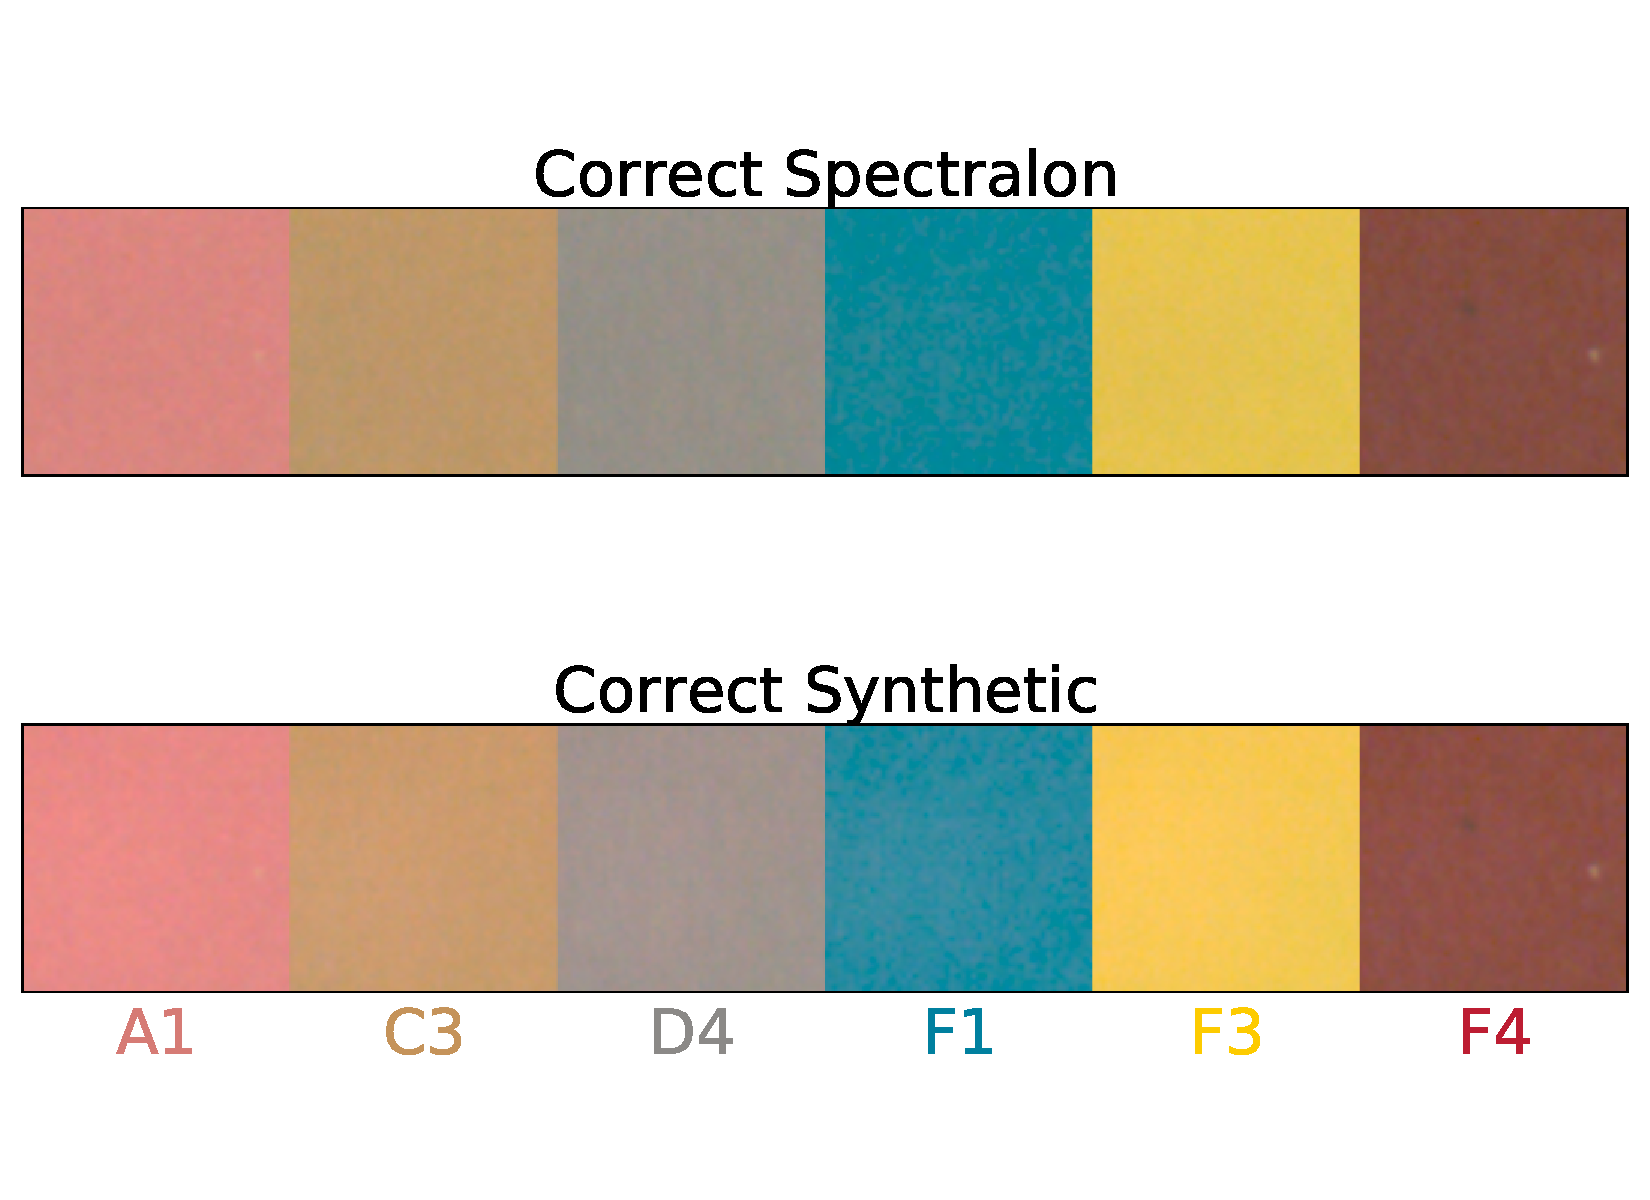
\includegraphics[width=0.7\textwidth]{Figure8}
	    % \label{fig:20Synthetic}
	% \end{subfigure}
    \caption{sRGB reconstructions of the central 200 x 200 pixels of a selection of tiles (labelled below as corresponding to those in \figref{fig:setup}b) taken at 20 cm and balanced with either the correct Spectralon white reference image, or the synthetic reference generated from the correct video of the sterile ruler.}
    \label{fig:summaryspectrasynthetic}
\end{figure}
% 
% 	
% 	
% 		
% 		
% 		
% 		
% 		
% 		
% 		
% 		
% 		
% 		
% 	
% 	
% 

\begin{table}[tbh!]
	\caption{Table showing the MedAPE (3sf) in the spectral sensitivities and in the pixel-by-pixel percentage errors (3sf) between the synthetic reference generated from a video of the sterile ruler and the reflectivity corrected Spectralon reference for each distance, alongside the mean $\NRMSE$ (3sf) when balancing with each synthetic reference for the quantitative and relative datasets for the mean measured spectrum of each tile compared to its spectrometer measurement, alongside the median pixel-by-pixel $\Delta E$ value (3sf) between the composite checkerboard CIELAB reconstruction and the literature values.}
	\csvloop{
		file = CombinedSyn.csv, 
		head to column names, 
		before reading = \centering\sisetup{table-alignment-mode=none, table-number-alignment=center, round-mode=figures, round-precision=3, separate-uncertainty=true},
		tabular={|l|S|S|S|S|S@{}c|}, 
		table head = \hline
		\textbf{Distance} & \multicolumn{2}{|c}{\textbf{MedAPE (\%)}} & \multicolumn{2}{|c|}{\textbf{$\NRMSE$}} & \textbf{$\Delta E$} & \\
		 \textbf{(cm)} & \textbf{$S_n$} & \textbf{pixel-by-pixel} & \textbf{Quantitative (\%)} & \textbf{Relative (a.u.)} &  & \\
		\hline, 
		command = \Distance & \Checkerss & \Checkerpbp & \quantNormRMSEa &  \normNormRMSEa & \quantmedianDeltaE & , 
		table foot = \hline , 
	}
	\label{tb:SynTotErrors}
\end{table}
\newpage
These synthetic references are also used to balance the checkerboard data as in \secref{methodmotivation} and the corresponding errors calculated. The results are summarized in \figref{fig:summaryspectrasynthetic}, and \tabref{tb:SynTotErrors} shows the resulting errors when using synthetic references. These show very similar errors compared to the best practice method suggesting that these synthetic references are suitable for quantitative data reconstruction. Since this process is fully sterile, it can be repeated easily during surgery allowing for changes in distance and lighting conditions to be better accounted for.
% 
% 	
% 	
% 	    
% 	    
% 	
	% 
	%     
	%     
	%     
	% 
% 
% 	    
% 	   
% 	    
% 
% 
% 
%    
% 	
	% 
	%   
	%    
	%    
	% 
	% 
	%    
	%   
	%    
	% 
	%
	%   
	%  
	% 
% 	
% 	
% 
% 
% 
% 	
% 		
% 		
% 		
% 		
% 		
% 		
% 		
% 		
% 		
% 		
% 		
% 		
% 	
% 	
% 
% 
% 	
% 	
% 		
% 		
% 		
% 		 
% 		
% 	
% 	
% 		
% 		
% 	
% 	
%

\FloatBarrier
For relative data, the spectral sensitivities are calculated from a single image of the ruler and used to balance the data. The spectral sensitivities of the Karl Storz D light C Xenon light source are used to balance the data before normalising and the resulting spectra are summarized in \figref{fig:NormSpecsens} and the corresponding errors in \tabref{tb:NormSpecsens}. This shows that spectral sensitivities alone are sufficient for white balancing of relative data.
\begin{figure}[htp!]
	\centering
        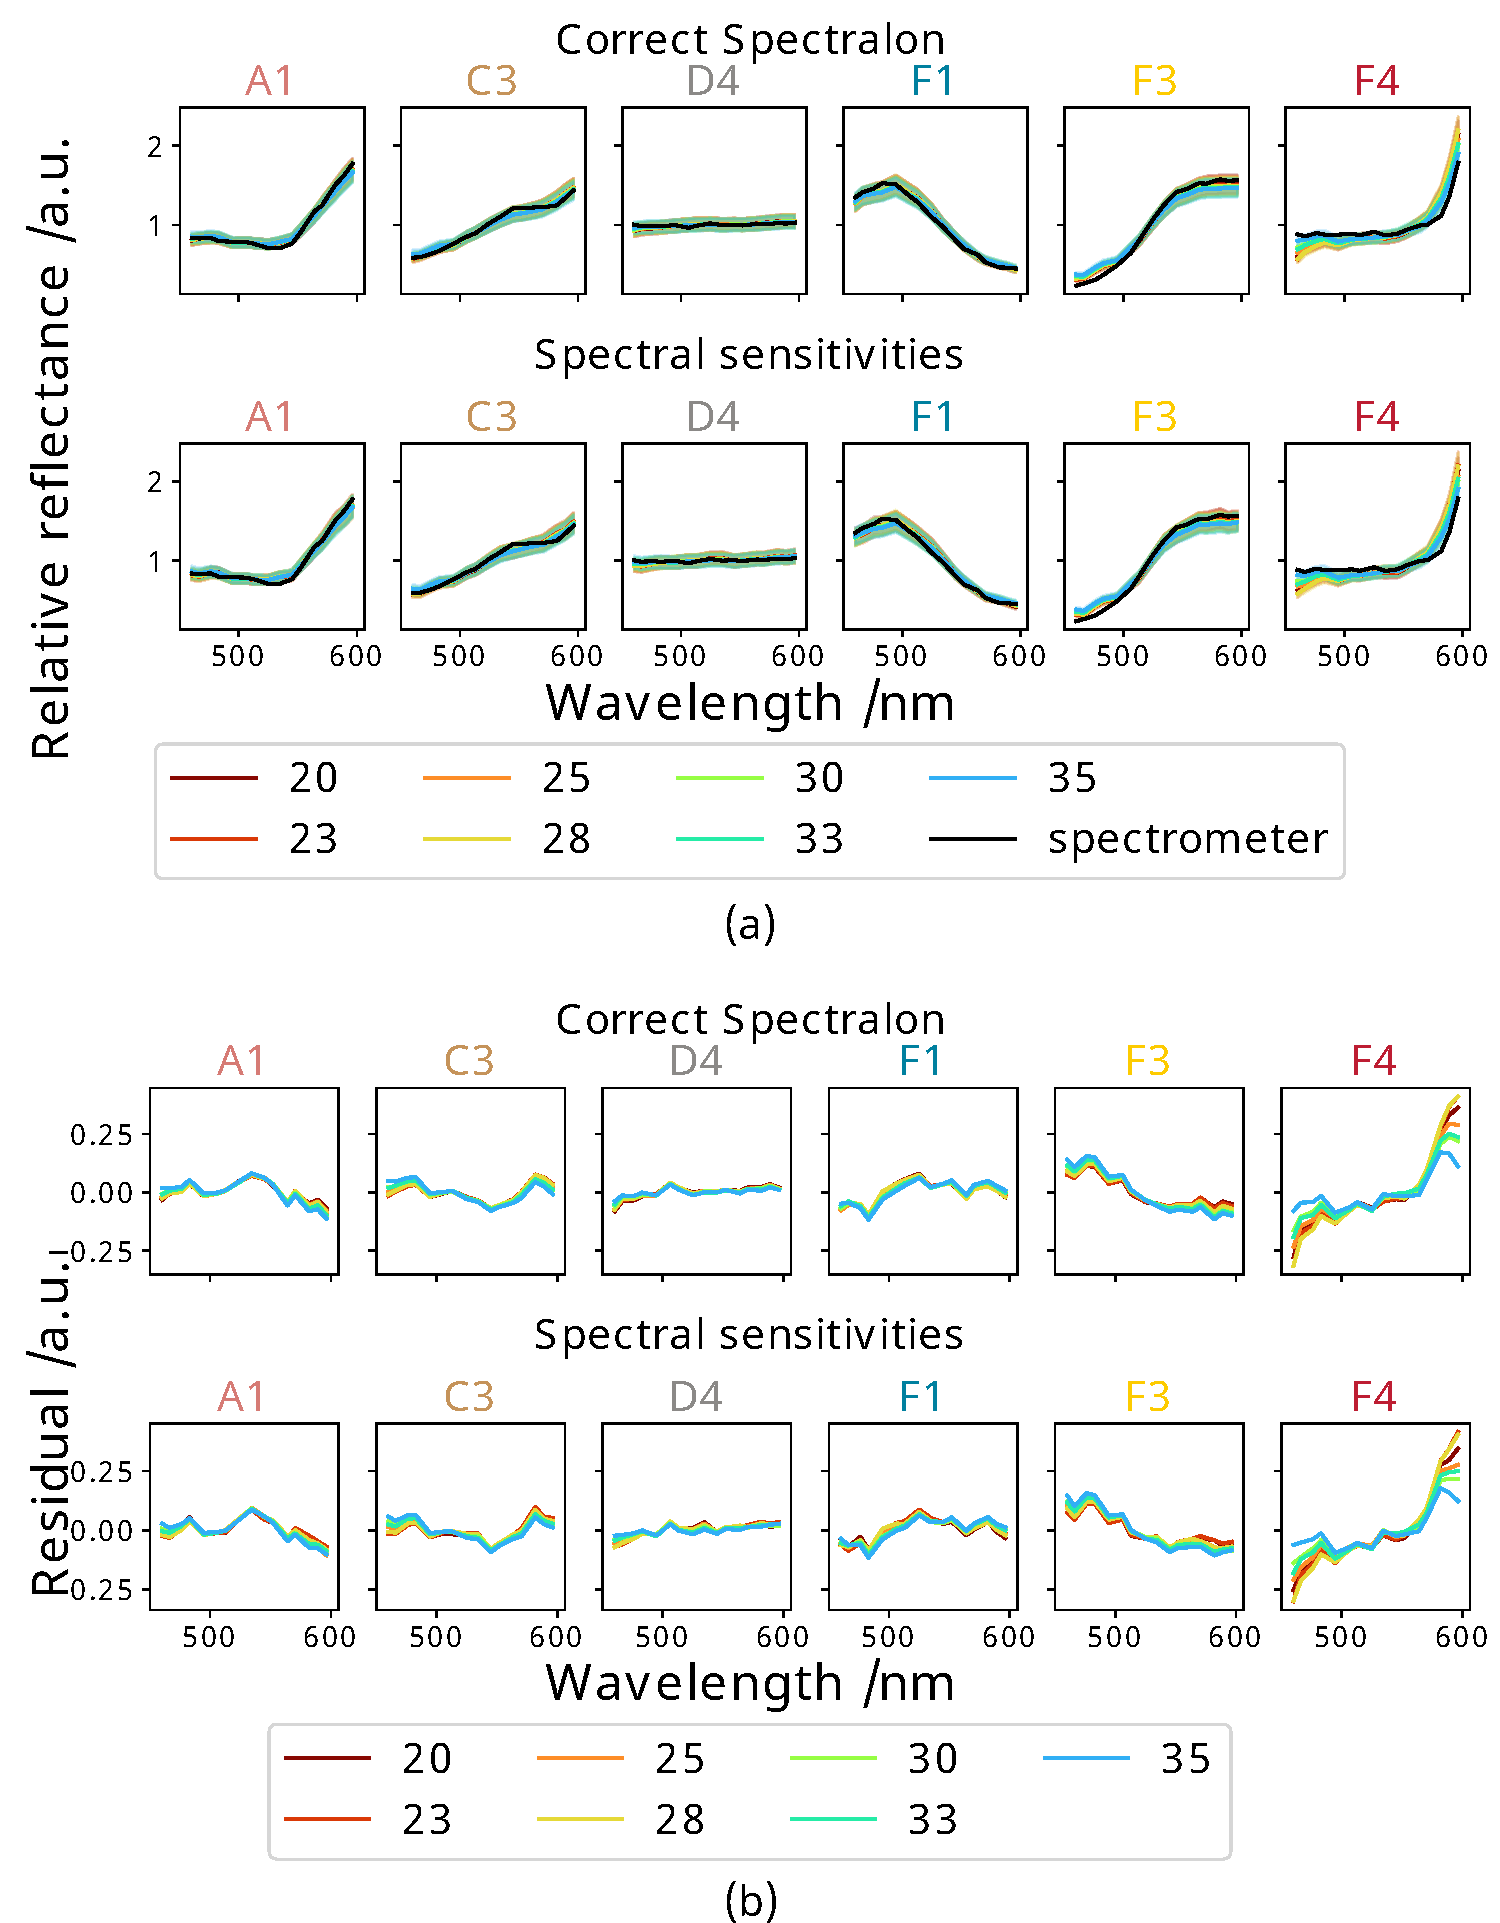
\includegraphics[width=\textwidth]{Figure9}
	% \begin{subfigure}[ht!]{0.77\textwidth}
	%     \includegraphics[width=\textwidth]{Figure9a}
	%     \caption{}
	%     \label{fig:NormSpecsensspectrum}
	% \end{subfigure}
	% \begin{subfigure}[ht!]{0.77\textwidth}
	%     \includegraphics[width=\textwidth]{Figure9b}
	%     \caption{}
	%     \label{fig:NormSpecsensresid}
	% \end{subfigure}
	\caption{(a) The relative mean spectrum of a selection of tiles as measured from each distance (cm) plotted against the spectrometer measurement of that tile, where each plot represents a new tile (labelled above it) as corresponding to the labels in \figref{fig:setup}b, and (b) their respective residuals compared to the spectrometer ground truths. All distances of checkerboard data are white balanced with either the correct measured white reference or the spectral sensitivities generated from a single image of the sterile ruler.}
	\label{fig:NormSpecsens}
\end{figure}
\begin{table}[htp!]
	\caption{Table showing the $\NRMSE$ (3sf) when balancing with the spectral sensitivities generated from a single image of a sterile ruler for the mean measured spectrum of each tile compared to its spectrometer measurement.}
	\csvloop{
		file = NormSpecsens.csv, 
		head to column names, 
		before reading = \centering\sisetup{table-alignment-mode=none, table-number-alignment=center, round-mode=figures, round-precision=3, separate-uncertainty=true},
		tabular={|l|S@{}c|}, 
		table head = \hline \textbf{Distance (cm)} & \textbf{$\NRMSE$ for} & \\
	& \textbf{Relative Spectra (a.u.)} & \\
	\hline, 
		command = \Distance & \normNormRMSEa & , 
		table foot = \hline, 
	}
	\label{tb:NormSpecsens}
\end{table}

\FloatBarrier
\subsubsection{Integration into a surgical environment}
\label{resultsintegration}
Our proposed synthetic reference algorithm was easily integrated into surgical workflow of a human cadaveric spine surgery. The study was approved by the local ethics committee of the canton of Zurich, Switzerland, under the number BASEC 202-01196. The video capture was adjusted to use a snipped section of the ruler to fit within the surgical cavity and the camera was moved in contrast to the ruler to capture the video. In this setting this is an appropriate adjustment due to the near uniformity of the background tissue and even illumination of the cavity using a single light source.
The measured white reference was taken for comparison, where distance was judged based on a visual assessment of image focus. The mean absolute percentage errors in the spectral sensitivities is 0.852\% and median absolute percentage pixel-by-pixel errors is 4.77\% between the synthetic and Spectralon references, which show that the synthetic reference is very similar to the best case intraoperative measured Spectralon reference. The $\NRMSE$ between the quantitative spectra constructed using the Spectralon and synthetic references were calculated between the spectrum of each pixel in the content area. This had a range of 0\% to 0.356\% with a median of 0.055\% showing that these are extremely similar. sRGB reconstructions of the image balanced with both Spectralon white reference and a synthetic white reference are shown in \figref{fig:ZurichRGB}. The $\Delta E$ values were calculated for each pixel between CIELAB reconstructions of these images and displayed in \figref{fig:ZurichRGB} with a range between 0 and 16.17 and a median of 1.37 in the content area indicating a barely perceptible difference to the human eye. This suggests that a synthetic white reference performs similarly to the best case intraoperative Spectralon white reference, however it is much more easily integrated into surgical workflow allowing for changing conditions to be better accounted for. 

\begin{figure}[h!]
	\centering
	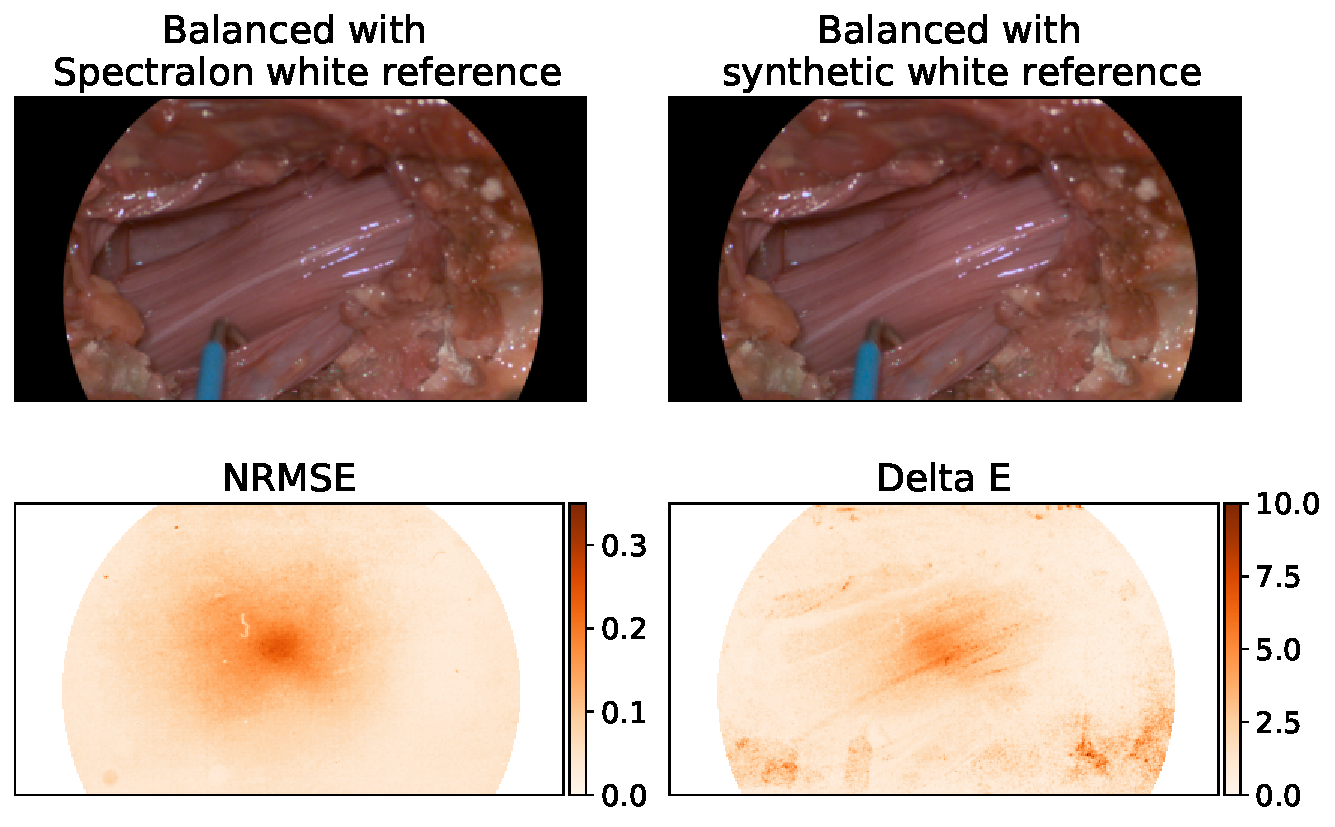
\includegraphics[width=\textwidth]{Figure10}
	\caption{sRGB reconstructions of human cadaveric rootlets balanced with a Spectralon reference and a synthetic white reference generated from a video of a sterile ruler against tissue, the pixel-by-pixel $\NRMSE$, and $\Delta E$ values calculated between the balanced spectra and CIELAB reconstructions of these. All images are masked due to the scope.}
	\label{fig:ZurichRGB}
\end{figure}

\FloatBarrier
\section{Discussion}
\label{conclusions}
This chapter first examined the limitations of white balancing under different conditions to the subject. The lack of a sterile reference necessitates that the white reference be taken outside of the sterile field. This means that the white reference may be taken at a different distance or under different lighting conditions to the subject. When investigating these effects, it is clear that there is little variation when data are correctly balanced, however changes in distance or lighting from the conditions of the white reference show appreciable differences. 

The change in distance primarily has an effect on quantitative data which is seen clearly at large differences in distance, however these changes are not seen in the sRGB reconstructions. The relative data is robust to changes in distance as this does not change the shape of the spectra, only the absolute intensity which is not relevant in calculation of ratiometric parameters. 

The change in lighting conditions has a severe effect on both quantitative and relative data as the shape of the spectra are altered. This effect is significant enough to be easily visually apparent in the sRGB reconstruction. 

The ability to model white references by separating the spatial and spectral components was then investigated. This produced relatively low inherent errors for all methods investigated. The approximation method modelling the vignetting as a two-dimensional isotropic Gaussian with the scalar factor and spectral sensitivities calculated was chosen to allow for imperfections in the composite reference whilst maximising computational efficiency. The spectral sensitivities in all three approximation methods showed no trends with distance, consistent with the assumption that the spatial and spectral effects can be treated separately. 

Synthetic references were generated from short videos of the ruler and compared to the relevant measured references. The errors in the spectral sensitivities and pixel-by-pixel values of the synthetic references compared to the appropriate measured references, of less than 6.5\%, suggest that there is little difference between the measured and synthetic references. 

When these synthetic references were used to balance the datasets at various distances, the results appeared similar to using appropriate measured references, with mean $\NRMSE$ for the quantitative spectra of 0.140\% and 0.139\% respectively. This demonstrates that these synthetic references can be used as an appropriate method of white balancing to obtain quantitatively accurate data. 

For relative data, only the shape of the spectra is relevant so only spectral sensitivities are required to white balance the data. For this the relevant spectral sensitivities are calculated once and used to balance the data across all datasets which results in very low errors. This shows that this simplified method of white balancing can be used in the case that relative data alone is required, however it is not possible to generate good sRGB reconstructions with only spectral sensitivities, since absolute intensity information is lost. 

The application of this method in a surgical environment was tested in a human cadaveric spine surgery. This demonstrated a simple integration into a surgical environment whilst producing similar spectra and sRGB reconstructions, with median $\NRMSE$ of 0.055\% and median $\Delta E$ of 1.37, and a synthetic reference that closely replicates the best case scenario using a standard reference. 

It is expected that this method can be integrated to a wide range of surgical applications where the exoscope can be held at a constant distance for the short ruler video, and the imaging of interest. This has been investigated for fronto-parallel distances of 20-35cm, which facilitates good ergonomics for neurosurgery by enabling the capture of a sufficiently wide field of view as well as resolving regions of interest in the depths of cavities, based on experience from the lead clinician on our neurosurgical study. Exposure should be set to prevent saturation of any wavelengths, however changes in exposure could be corrected linearly. If lighting is uniform across the field of view, this allows the video to be taken by movement of camera instead of reference, however shadows in the cavity can only be accounted for by movement of the reference itself.

This indicates a promising novel method for synthetic white balancing within the restricted intraoperative environment provided the assumption that spatial and spectral independence is held. This assumption is often met using a single, uniform light source. The quantitative model is currently limited to fronto-parallel imaging with the assumption that imaging geometry does not deviate significantly from this, which also introduces a limitation in its application, however relative data can be obtained at any angle in principle using the spectral sensitivities independently.

\subsection{Conclusions and future work}
These data demonstrate a novel sterile synthetic white balancing algorithm capable of integrating easily into surgical workflow. This ensures quantitative accuracy of the spectral data obtained, whilst minimising disruption to the surgical procedure.

Future work should include improvement of the computational efficiency of the composite ruler reference construction for a real-time integration of this method. It should be confirmed that this construction is robust to movement in the background as this enables the video to be obtained by movement of the camera in contrast to movement of the ruler, allowing this method to be more easily used in more restricted surgical cavities assuming an even illumination from a single light source. This method should also be adapted to be able to account for any dust in the system, multiple light sources, validation for the replacement of the exoscope with other operating scopes, validation for distances applicable to other open surgery geometries, and adaptation to use at different imaging angles.

The work in this chapter informs the clinical HSI data collection protocols used in the remainder of this thesis. 

% \begin{comment}
% \section*{Acknowledgements}
% This study/project is funded by the NIHR [NIHR202114]. The views expressed are those of the author(s) and not necessarily those of the NIHR or the Department of Health and Social Care.
% %
% This work was supported by core funding from the Wellcome/EPSRC [WT203148/Z/16/Z; NS/A000049/1].
% This project has received funding from the European Union's Horizon 2020 research and innovation programme under grant agreement No 101016985 (FAROS project).
% %
% CH is supported by an InnovateUK Secondment Scholars Grant (Project Number 75124).
% %
% TV is supported by a Medtronic / RAEng Research Chair [RCSRF1819\textbackslash7\textbackslash34].
% %
% For the purpose of open access, the authors have applied a CC BY public copyright licence to any Author Accepted Manuscript version arising from this submission.

% \section*{Data availability statement}
% The datasets presented in this article are not readily available because of their proprietary nature.

% % \section*{Disclosure statement}
% % ME, JS and TV are co-founders and shareholders of Hypervision Surgical.
% %
% %TV holds shares from Mauna Kea Technologies.
% % \end{comment}
\FloatBarrier
%
%
%
\typeout{}
% \bibliography{Main_body}
% \doublespacing
% \listoffigures

% \iffalse
% \section*{Biographies}
% Anisha Bahl is a PhD student in the Surgical and Interventional Engineering department of King's College London. She received her Chemistry MChem in 2020 from the University of Oxford. Her main research interests are the integration of spectral measurement and imaging technologies to medical settings, and the extraction of physiological information from these technologies to aid medical decision making. 
% \fi
% 
% \end{document}

% \PassOptionsToPackage{dvipsnames}{xcolor}

% \documentclass[ACS,STIX1COL]{WileyNJD-v2}
% \usepackage{moreverb}
% \usepackage{graphicx} % Required for inserting images
% %\usepackage{xcolor}
% \definecolor{MyGreen}{RGB}{141,208,138}
% \definecolor{MyBlue}{RGB}{134,190,220}
% \definecolor{MyOrange}{RGB}{252,128,96}
% \definecolor{MyPurple}{RGB}{174,173,211}

% \usepackage{amsmath}
% \usepackage{multirow}
% \usepackage{placeins}
% \usepackage{subcaption}
% \captionsetup[figure]{labelfont=normalsize}

% \usepackage{marginnote}
% %\newcommand{\revref}[2]{\marginnote{$R_{#1}C_{#2}$}}
% %\newcommand{\revref}[2]{\marginpar[$R_{#1}C_{#2}$]{}}
% \newcommand{\revref}[2]{\marginnote{\textcolor{purple}{$R_{#1}C_{#2}$}}}
% %\setlength{\marginparsep}{10mm}
% \setlength{\marginparwidth}{15mm}
% %\usepackage{everyshi}

% \articletype{article}

% \graphicspath{ {./Figures/} }

% \begin{document}

\chapter[A comparative study of single layer analytical models]{A comparative study of analytical models of diffuse reflectance in homogeneous biological tissues: Gelatin based phantoms and Monte Carlo experiments.}\label{chap:1layer}
% \author[1]{Anisha Bahl*}
% \author[1]{Silvere Segaud}
% %\author[1]{Jenasee Mynerich}
% \author[1]{Yijing Xie}
% \author[1,3]{Jonathan Shapey}
% \author[2]{Mads S. Bergholt}
% \author[1]{Tom Vercauteren}

% \address[1]{\orgdiv{School of Biomedical Engineering \& Imaging Sciences}, 
% \orgname{King's College London}, 
% \orgaddress{1 Lambeth Palace Road, London, United Kingdom}}
% \address[2]{\orgdiv{Department of Craniofacial Development and Stem Cell Biology}, 
% \orgname{King's College London}, 
% \orgaddress{Guy's Tower, Great Maze Pond, London, United Kingdom}}
% \address[3]{\orgname{King's College Hospital}, 
% \orgaddress{Denmark Hill, London, United Kingdom}}


% \corres{*Anisha Bahl, School of Biomedical Engineering \& Imaging Sciences, King's College London, 1 Lambeth Palace Road, London, United Kingdom. \email{anisha.bahl@kcl.ac.uk}}

\begin{center}
\begin{minipage}[b]{0.9\linewidth}
\small
\textbf{Foreword\,}
This chapter is an \emph{in extenso} reproduction of \cite{Bahl2023a} and has been submitted to Journal of Biophotonics for publication. 
\newline
AB identified the three major analytical tissue models for comparison, designed and conducted the simulations and synthetic experiments and measurements to construct the datasets for evaluation, and conducted the evaluation of the models under the supervision of JS, MB, and TV. AB worked collaboratively with SS and YX to identify and validate the appropriate IAD method to use in this work. 
\end{minipage}
\end{center}

\minitoc

% \abstract[Abstract]{
% Information about tissue oxygen saturation ($StO_2$) and other related important physiological parameters can be extracted from diffuse reflectance spectra measured through non-contact imaging.
% %Tissue oxygen saturation ($StO_2$) is an important physiological parameter, and it has been proposed that this could be extracted from diffuse reflectance spectra measured through non-contact imaging.
% %however there are no established, spatially-resolved, intra-operative methods to evaluate this. It has been proposed that $StO_2$ could be extracted from diffuse reflectance spectra measured through non-contact imaging. 
% Three analytical optical reflectance models for homogeneous, semi-infinite, tissue have been proposed (Modified Beer-Lambert, Jacques 1999, Yudovsky 2009) but these have not been directly compared for tissue parameter extraction purposes. 
% We compare these analytical models using Monte Carlo simulated diffuse reflectance spectra and 
% %measured, 
% controlled gelatin-based phantoms
% %diffuse reflectance spectra
% with
% %known ground truth.
% measured diffuse reflectance spectra and known ground truth composition parameters.
% %Our results were evaluated on goodness of fit and parameter extraction accuracy.
% The Yudovsky model performed best against Monte Carlo simulations and measured spectra of tissue phantoms in terms of goodness of fit and parameter extraction accuracy followed closely by Jacques' model. 
% In this study, Yudovsky's model appeared most robust, however our results demonstrated that both Yudovsky and Jacques models are suitable for modelling tissue that can be approximated as a single, homogeneous, semi-infinite slab.}

% \keywords{Biological models; Oxygen saturation; Monte Carlo simulations; Imaging phantoms; Gelatin}

% \maketitle 
% 
\section{Introduction}\label{sec:intro}
As mentioned in Chapter \ref{chap:intro}, $StO_2$ 
%Tissue oxygen saturation ($StO_2$) 
is a key metric that could be used in surgery to determine tissue viability, tumour localisation, and vessel flow \cite{Takami2017, Hughes2019, Richardson2023}.
There are, however, no currently established, spatially-resolved, intra-operative methods of quantitatively determining $StO_2$ and so perfusion is often displayed (e.g. using DSA, MVD, or ICG) or global $StO_2$ is discussed from JVOS or cerebral oximetry.
% In many clinical applications indocyanine green fluorescence angiography (ICG) is used to display perfusion as 
% %oxygenated
% blood flow through vessels can be visualised by the fluorescence of the indocyanine dye given to the patient \cite{Hackethal2018}.
% Whilst this method has shown clinical benefits \cite{Renna2023, Teng2021}, it cannot quantify the $StO_2$ of the tissues being visualised leading to subjective interpretation.
There has been increasing promise that diffuse reflectance spectroscopic techniques could be used to obtain $StO_2$ intra-operatively. Hyperspectral Imaging (HSI) is one such technique that obtains a diffuse reflectance spectrum for each pixel of an image \cite{Kulcke2018, Taylor-Williams2022}, enabling intra-operative, non-contact, spatially-resolved $StO_2$ extraction without the need for a contrast agent. 

There have been many proposed methods to extract $StO_2$ parameters from tissue diffuse reflectance spectra ranging in complexity, as mentioned in Chapter \ref{chap:intro}.
%from the simplest ratiometric two-wavelength methods to more sophisticated analytical models \cite{MacKenzie2018} or deep-learning based approaches \cite{Ayala2023}. Using two or three wavelength models can provide good results but require data to be captured at these precise wavelengths placing large constraints on the measurement devices used and significant model assumptions. 
Analytical models can be applied to ranges of wavelengths for which they are developed and so these are favoured in this work. 
%\revref{2}{6}\textcolor{red}{
Here we consider only visible range models (450-650nm) as this allows for non-contact imaging using standard cold surgical light sources \cite{Clancy2011}.
The visible light wavelength range also penetrates less deeply into tissue \cite{Eggert1987, Sabino2016}. Light-tissue interaction is therefore most likely to replicate a single homogeneous semi-infinite tissue layer and less likely to travel between layered structures.
%}
Tissue models tend to either be based on modifications of the Beer-Lambert model, or on the diffusion approximation particularly using the Kulbelka-Munk approximation method\cite{MacKenzie2018}. Three models that can be applied to homogeneous semi-infinite tissue in the visible wavelength range (450-650nm) include 1) a modified Beer-Lambert model \cite{Clancy2015}; 2) a more elaborate Beer-Lambert-based model proposed by Jacques \cite{Jacques1999}; and 3) a semi-empirical model based on the Kulbelka-Munk theory as described by Yudovsky \cite{Yudovsky2009}.
Alternatively, Monte Carlo (MC) methods may be used to model tissues for a range of wavelengths. Whilst MC is an established approach for modelling light-tissue interaction, it is computationally challenging to apply in an inverse problem setting making the estimation of optical properties from tissue spectra non trivial on the basis of MC simulations alone.
To address the need for improved inverse modelling utilising MC, Inverse Adding Doubling (IAD)\cite{Prahl2017} has been proposed, however this is also slow iterative process and therefore not as efficient as approaches based on analytical models.
A limitation of IAD is that, although a single reflectance measurement can be used to analyse semi-infinite samples with IAD, its primary focus is the extraction of optical properties from slabs of tissue with known thickness using both transmission and reflection measurements.
In this chapter, IAD is used to provide information on optical properties from tissue phantom slabs but is not assessed in the same capacity as the other 
%other purely
analytical models listed above. 

Since there is no standard method of determining spatially resolved, ground truth, optical properties of tissues, 
simulations and physical
phantoms must be used
%to test analytical models.
for testing purposes.
Gelatin-based phantoms are commonly used to allow tunable absorption and scattering properties in solid phantoms \cite{Pogue2006, Gautam2023}.
%
In this chapter we compare three major analytical models against both MC simulated spectra, and measured spectra from gelatin-based tissue phantoms with known ground-truth constituent quantities. These datasets cover a large parameter range mimicking that expected in biological tissue\cite{Jacques2013}. Gelatin phantoms are constructed to optically mimic biological tissue absorption and scattering ranges as closely as possible, whilst maintaining well-defined optical properties with known ground truth. We present a first direct comparison in the performance of these models against simulated and measured spectra, and aim to evaluate their potential for accurate $StO_2$ extraction. This evaluation is quantified in terms of the forward models (utilising ground truth values within the models to predict the diffuse reflectance spectra), and for the inverse problem solving (evaluating the fidelity of the parameter extraction when fitting to the simulated or measured data).
Our results provide a comparison which can be used to inform the translation of these models into clinical applications.

\section{Materials and methods}\label{sec:methods}
\subsection{Tissue models}\label{sec:methodtissuemodels}
Three analytical models are compared and evaluated in this work: modified Beer-Lambert \cite{Clancy2015}, Jacques 1999 \cite{Jacques1999}, and Yudovsky 2009 \cite{Yudovsky2009}. Due to the absorbing and scattering nature of biological tissue these models are used to analyse diffuse reflectance spectra which result from propagation of light via many optical paths through the tissue.
% \begin{figure}
%     \centering
%     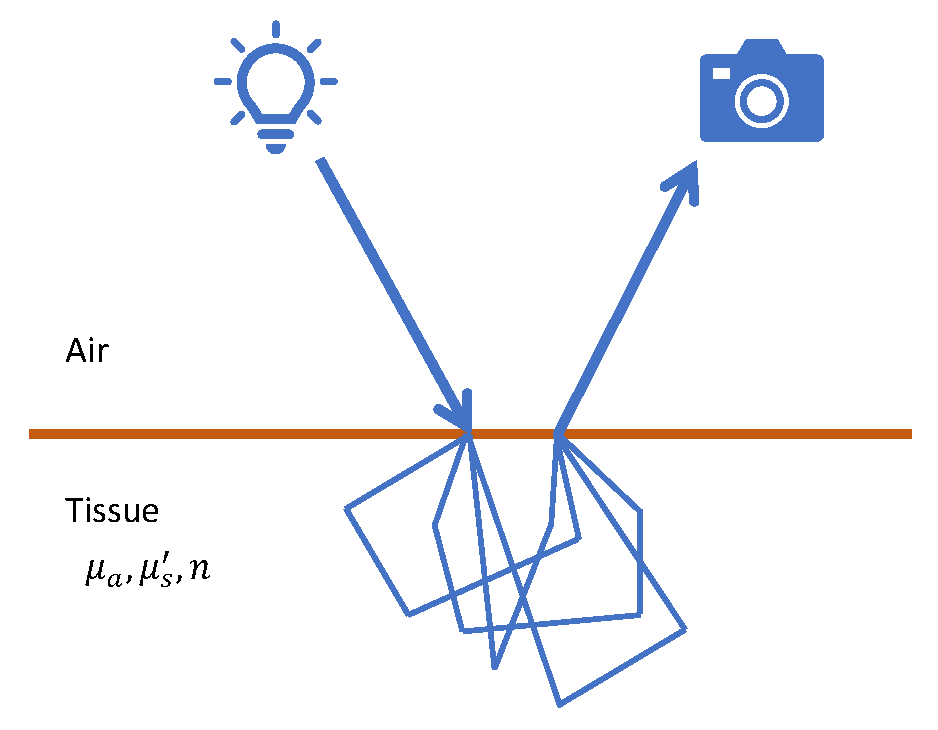
\includegraphics[width=0.4\textwidth]{TissueFigure.pdf}
%     \caption{Diagram depicting the multiple paths taken through tissue before the light exits to be detected as diffuse reflectance.}
%  \label{fig:tissuefigure}
% \end{figure}

\subsubsection{Common absorption and scattering model}\label{sec:opticproperties}
All three forward models use the wavelength dependent absorption and reduced scattering coefficients ($\mu_a(\lambda)$ and $\mu_s'(\lambda)$) of the tissue as inputs
%and output
to compute a
diffuse reflectance spectrum. 
The reduced scattering coefficient comprises of the scattering coefficient ($\mu_s(\lambda)$) and tissue anisotropy ($g$) as follows: 
\begin{equation}
    \mu_s'(\lambda) = \mu_s(\lambda) \times (1-g)
    \label{eq:reducedscattering}
\end{equation}
For biological tissue, the reduced scattering coefficient can be well approximated using Mie theory \cite{Jacques2013}: 
\begin{equation}
    \mu_s'(\lambda) = a(\frac{\lambda}{500})^{-b}
    \label{eq:Mie}
\end{equation}
where $a$ and $b$ are Mie scattering coefficients that range between 8\textrm{$cm^{-1}$} and 70\textrm{$cm^{-1}$}, and 0.1 and 3.3 respectively depending on the tissue microstructure \cite{Jacques2013}. 
The absorption coefficient of most internal, homogeneous, single-layer tissues is dominated by haemoglobin in the visible region (450-650 nm)\cite{JacquesAbs} and can be modelled using the following equation \cite{Yudovsky2009}: 
\begin{equation}
\begin{aligned}
    & \mu_a(\lambda) = f_{blood}\mu_{a, blood}(\lambda) + (1 - f_{blood})\mu_{a, back}(\lambda) \\
    & \textrm{where} \\
    & \mu_{a, blood}(\lambda) = c_{HbT}\frac{\ln(10)}{64500}[StO_2 \epsilon_{HbO_2}(\lambda) + (1 - StO_2)\epsilon_{Hb}(\lambda)] \\
    & \textrm{and} \\
    & \mu_{a, back}(\lambda) = 7.84\times10^8 \lambda^{-3.255}
\end{aligned}
\label{eq:mua}
\end{equation}
Here $StO_2$ refers to oxygen saturation, $c_{HbT}$ refers to the total concentration of haemoglobin in whole blood commonly taken as 150\textrm{$gL^{-1}$}\cite{Prahl1999}, with $StO_2$ denoting the fraction of this that is oxygenated ($HbO_2$) and the remainder is deoxygenated ($Hb$), and ranges between 0-100\%\cite{Yudovsky2009}. $f_{blood}$ is the volume fraction of tissue occupied by blood which has absorption coefficient $\mu_{a, blood}(\lambda)$ and is examined in the range of 0.2-7\%\cite{Yudovsky2009}, with the remainder of tissue having background absorption $\mu_{a, back}(\lambda)$\cite{Yudovsky2009}.
Finally, $\epsilon_{HbO_2}(\lambda)$ and $\epsilon_{Hb}(\lambda)$ denotes the wavelength-dependent extinction coefficients of the chromophores $HbO_2$ and $Hb$ which are found in the literature\cite{Prahl1999}. 

\subsubsection{Modified Beer-Lambert}
The modified Beer-Lambert utilises these inputs to model absorption ($A(\lambda)$) and diffuse reflectance ($R(\lambda)$) as follows: 
\begin{equation}
\begin{aligned}
    & A(\lambda) = L\mu_a(\lambda) + \mu_s'(\lambda) \\
    & R(\lambda) = \exp{\left(-\frac{A(\lambda)}{100}\right)}
\end{aligned}
\label{eq:modBL1}
\end{equation}
Conventionally, $\mu_a(\lambda)$ and $\mu_s'(\lambda)$ are quoted in units of cm\textrm{$^{-1}$}, however in this model units of mm\textrm{$^{-1}$} are required for diffuse reflectance units of \% hence a factor of 100 is included. $L$ describes a differential path length to account for the variety of photon path lengths through scattering media. $L$ is often simplified to be equal to 1 \cite{Clancy2015} and $\mu_s'(\lambda)$ is often modelled as a wavelength-independent constant\cite{Clancy2015, Ma2016}. 
To allow for further flexibility in this model,
we introduce linear scaling hyperparameters ($M_{1-3}$), as shown in Equation \eqref{eq:modBL2}, that can be fitted to MC simulations at the refractive index of interest. 
\begin{equation}
\begin{aligned}
    & A(\lambda) = M_1\mu_a(\lambda) + M_2\mu_s'(\lambda) + M_3 \\
    & R(\lambda) = \exp{\left(-\frac{A(\lambda)}{100}\right)}
\end{aligned}
\label{eq:modBL2}
\end{equation}

\subsubsection{Jacques 1999}\label{sec:Jacques}
The Jacques model is also based on the Beer-Lambert model, where an assumption is made that the ensemble of path lengths experienced by photons in a tissue can be approximated by a single wavelength-dependent path length $L(\lambda) = A(\lambda)\delta(\lambda)$ where $A(\lambda)$ and $\delta(\lambda)$ are defined in Equation \ref{eq:Jacques}. This results in the following model with the hyperparameters ($M_{1-3}$) which the authors
%state are fitted
fit
to Adding Doubling simulations \cite{Jacques1999}. In our work, we refit these to MC simulations since these are considered the gold standard optical simulation method and improve the model fitting results. 
\begin{equation}
\begin{aligned}
    & N'(\lambda) = \frac{\mu_s'(\lambda)}{\mu_a(\lambda)} \\
    & \delta(\lambda) = \frac{1}{\sqrt{3\mu_a(\lambda)[\mu_a(\lambda) + \mu_s'(\lambda)]}} \\
    & A(\lambda) = M_1 + M_2\exp \left[ \frac{\ln(N'(\lambda))}{M_3} \right] \\
    & R(\lambda) = \exp[-A(\lambda)\delta(\lambda)\mu_a(\lambda)] \\
\end{aligned}
\label{eq:Jacques}
\end{equation}

\subsubsection{Yudovsky 2009}\label{sec:Yudovskysingle}
The original Yudovsky model presents a complex analytical derivation \cite{Yudovsky2009} with a simplified formulation subsequently presented in their Erratum \cite{Yudovsky2015}. The model takes the reduced albedo ($w'(\lambda)$) as input and returns the diffuse reflectance spectra ($R(\lambda)$). This provides an easily applicable model with hyperparameters ($M_{1-6}$) which are quoted for a refractive index ($n$) of 1.44. We found that these can be fitted to MC spectra to allow for use with other refractive indices. 
\begin{equation}
\begin{aligned}
    & w'(\lambda) = \frac{\mu_s'(\lambda)}{\mu_a(\lambda) + \mu_s'(\lambda)} \\
    & R = M_1 + M_2\exp{\left[ M_3w'(\lambda)^{M_4}\right]} + \frac{M_5}{1.02 - M_6} \\
\end{aligned}
\label{eq:Yudovskysingle}
\end{equation} 

\subsubsection{Fitting model hyperparameters}
All analytical models considered use hyperparameters to account for the media's refractive index. A MC dataset is generated for each refractive index as in Section \ref{sec:methodsMC}. To fit the hyperparameters, the ground truth tissue parameters are inputted into an analytical model for each spectrum in the dataset and a single set of hyperparameters are fitted using a non-linear least squares fitting approach.

\subsection{Generating reference datasets of diffuse reflectance spectra}\label{sec:methodreference}
In this work, we aim to compare the three models discussed in Section \ref{sec:methodtissuemodels} against datasets with known ground truth. These datasets of diffuse reflectance spectra are generated either by simulation using MC (Section \ref{sec:methodsMC}) or measurement of controlled, gelatin-based, tissue phantoms (Section \ref{sec:methodsphantoms}).

\subsubsection{Monte Carlo simulations}\label{sec:methodsMC}
The models take $\mu_a(\lambda)$ and $\mu_s'(\lambda)$ as inputs. These are given for bulk tissue in Equations \eqref{eq:mua} and \eqref{eq:Mie} and used to generate MC simulated reference spectra. MC takes $\mu_s(\lambda)$ as input, not $\mu_s'(\lambda)$, so a random value of anisotropy ($g$) is chosen per spectrum between 0.7-0.9\cite{Yudovsky2009} and used in Equation \eqref{eq:reducedscattering} for conversion to $\mu_s(\lambda)$. The variable parameters are $a$, $b$, $StO_2$, and $f_{blood}$ which are bounded to 8-70cm\textrm{$^{-1}$}, 0.1-3.3, 0-100\%, 0.2-7\% respectively to mimic biological tissue\cite{Yudovsky2009, Jacques2013}; a value of each of these variables is randomly selected within these bounds to generate each of the 100 simulated spectra, meaning 100 values of each parameter are sampled. When fitting the inverse models to these spectra for parameter extraction (as described in Section \ref{sec:methodevaluate}), the same bounds are imposed on the fitting routine. These simulated spectra are generated using CUDAMCML\cite{Alerstam2008}, which is a GPU accelerated adaptation of the well-established MCML programme\cite{Wang1995}. It has been shown that the semi-infinite approximation is valid for thicknesses of above 1cm\cite{Zhang2014} so 100 spectra were simulated for each refractive index of 1.33, 1.35, and 1.44, by propagating 100,000 photons through the semi-infinite slabs approximated by a thickness of 3cm. The refractive indices were chosen to represent the common phantom and tissue use-cases of these models: 1.33 for use with water-based phantoms, 1.35 for use with gelatin-based phantoms (as in this work), and 1.44 for use with biological tissue.

\subsubsection{Controlled gelatin-based tissue phantoms}\label{sec:methodsphantoms}
Here we construct controlled, optical tissue phantoms with well-characterised components. By measuring these phantoms we constructed a dataset of measured spectra with well-defined ground truth which can be modelled using the analytical models.

\paragraph{Phantom composition and synthesis}\label{sec:methodsphantomcomposition}
% First the components of the optical tissue phantoms are detailed, with the full synthetic method found on page \pageref{sec:methodsphantomsynthesis}.

The dyes acid red 1 (AR1, 210633, Merck, Germany) and acid red 14 (AR14, B22328, Fisher Scientific, England) are chosen to mimic the extinction coefficients of oxygenated and deoxygenated haemoglobin respectively, with a third dye of crystal violet (CV, C6158, Merck, Germany) chosen to investigate the effect of including further chromophores. As in the modelled tissue $\mu_a(\lambda)$ (Equation \eqref{eq:mua}), the total dye concentration is modelled independently of the relative ratios of each dye. To ensure the absorbance impact of each dye is approximately equal, a factor of $\frac{5}{3}$ is included for AR14 and $\frac{1}{2}$ for CV computationally by combining with the extinction coefficients to create effective extinction coefficients ($\epsilon_{eff}$) that have approximately equal impact. To reflect this experimentally, the concentrations of these dyes are modified by these factors. These effective extinction coefficients calculated from literature values\cite{PhotochemCAD}, alongside those of haemoglobin\cite{Prahl1998}, can be seen in Figure \ref{fig:phantommethods}a. 
% \begin{figure}[h]
%     \centering
%     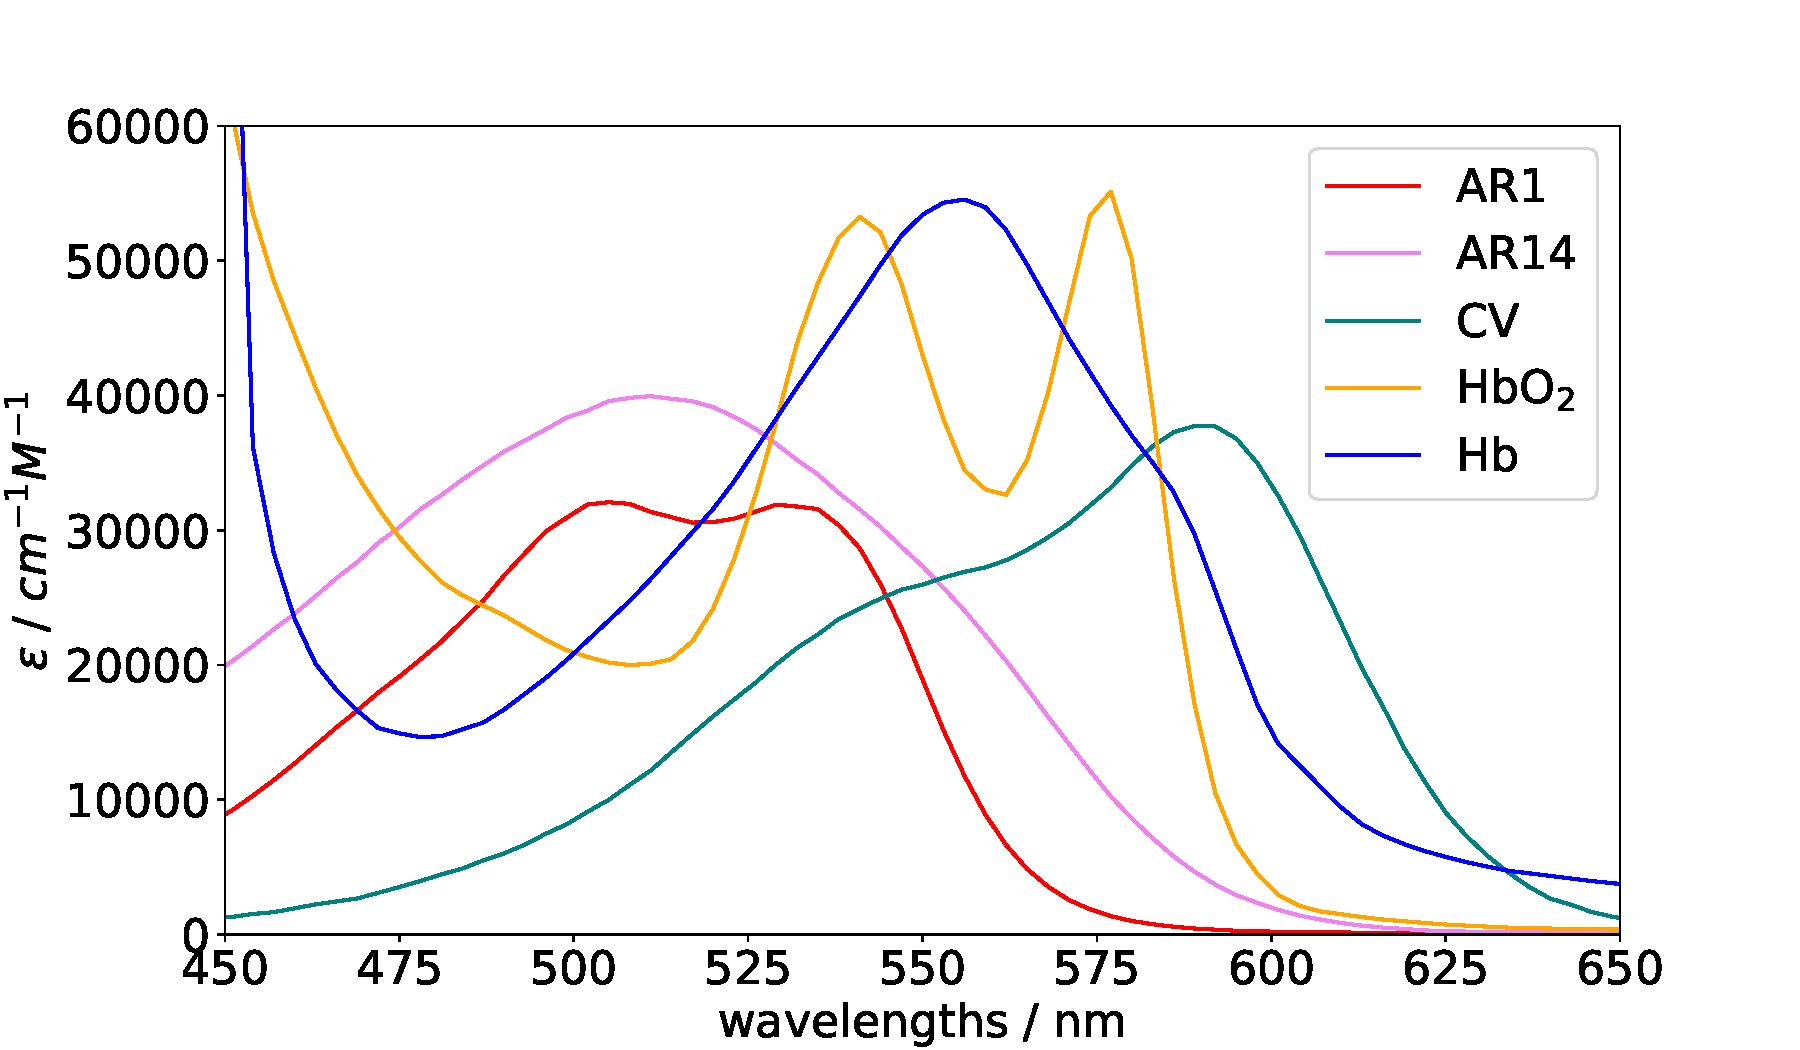
\includegraphics[width=0.6\textwidth]{effective_eps_lit.pdf}
%     \caption{Effective extinction coefficients of acid red 1 (AR1), acid red 14 (AR14), and crystal violet (CV) displayed with the extinction coefficients of oxygenated (HbO$_2$) and deoxygenated haemoglobin (Hb).}
%  \label{fig:exteff}
% \end{figure}

The tissue phantoms are constructed with three overall dye concentrations corresponding to fractions of blood of 0.344\%, 3.44\%, and 6.88\% ie. $8\times10^{-6}$ moldm$^{-3}$, $8\times10^{-5}$ moldm$^{-3}$, and $1.6\times10^{-4}$ moldm$^{-3}$. This can be described as a 1x, 10x, and 20x concentration with a scale factor of $8\times10^{-6}$.
Two-dye configurations are constructed to investigate a range of AR1:AR14 ratios with some 3-dye configurations added. 

Intralipid is used to modulate the scattering coefficient of these phantoms which can be modelled with a Mie scattering function (Equation \eqref{eq:Mie}) using parameters within the range of tissues. 5 volume fractions of intralipid are chosen between 1\% and 6\% to cover a range of scattering parameters within those seen in biological tissue \cite{Jacques2013}. 

Each phantom consists of 6\% gelatin (Type A approximately 175g bloom, G2625, Merck, Germany) by mass %to mimic the properties of healthy tissue \cite{Doyley2003} 
and 0.5\% of 4\% formaldehyde (J60401, Fisher Scientific, England) to increase the melting point of the phantoms and allow their use at room temperature \cite{Pogue2006}. The remainder of each phantom consists of the dye solutions in a variety of ratios combined with intralipid at a variety of concentrations. 

\begin{figure}[htb]
    \centering%\revref{1}{3}
    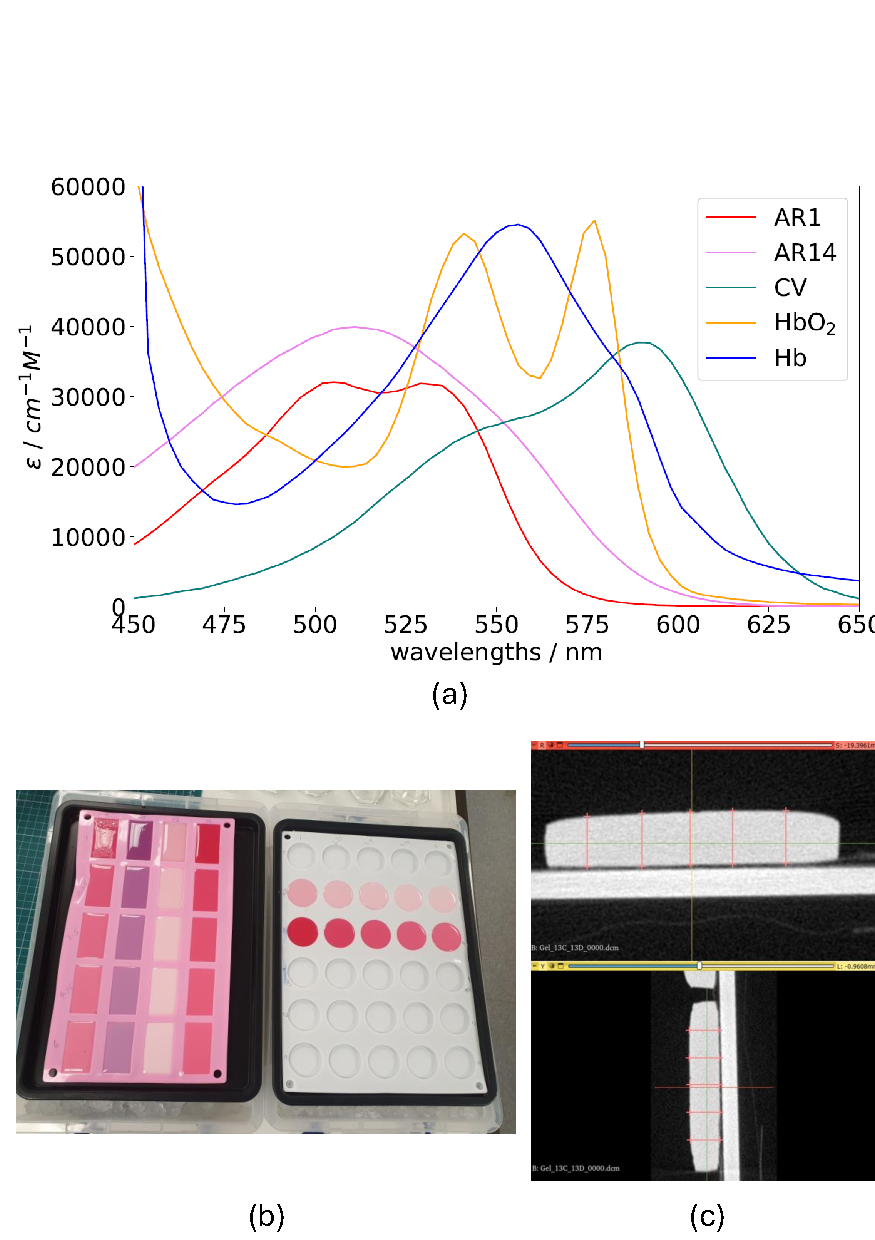
\includegraphics[width=0.5\textwidth]{Figure_1.pdf}
    % \begin{subfigure}{0.6\textwidth}
    %     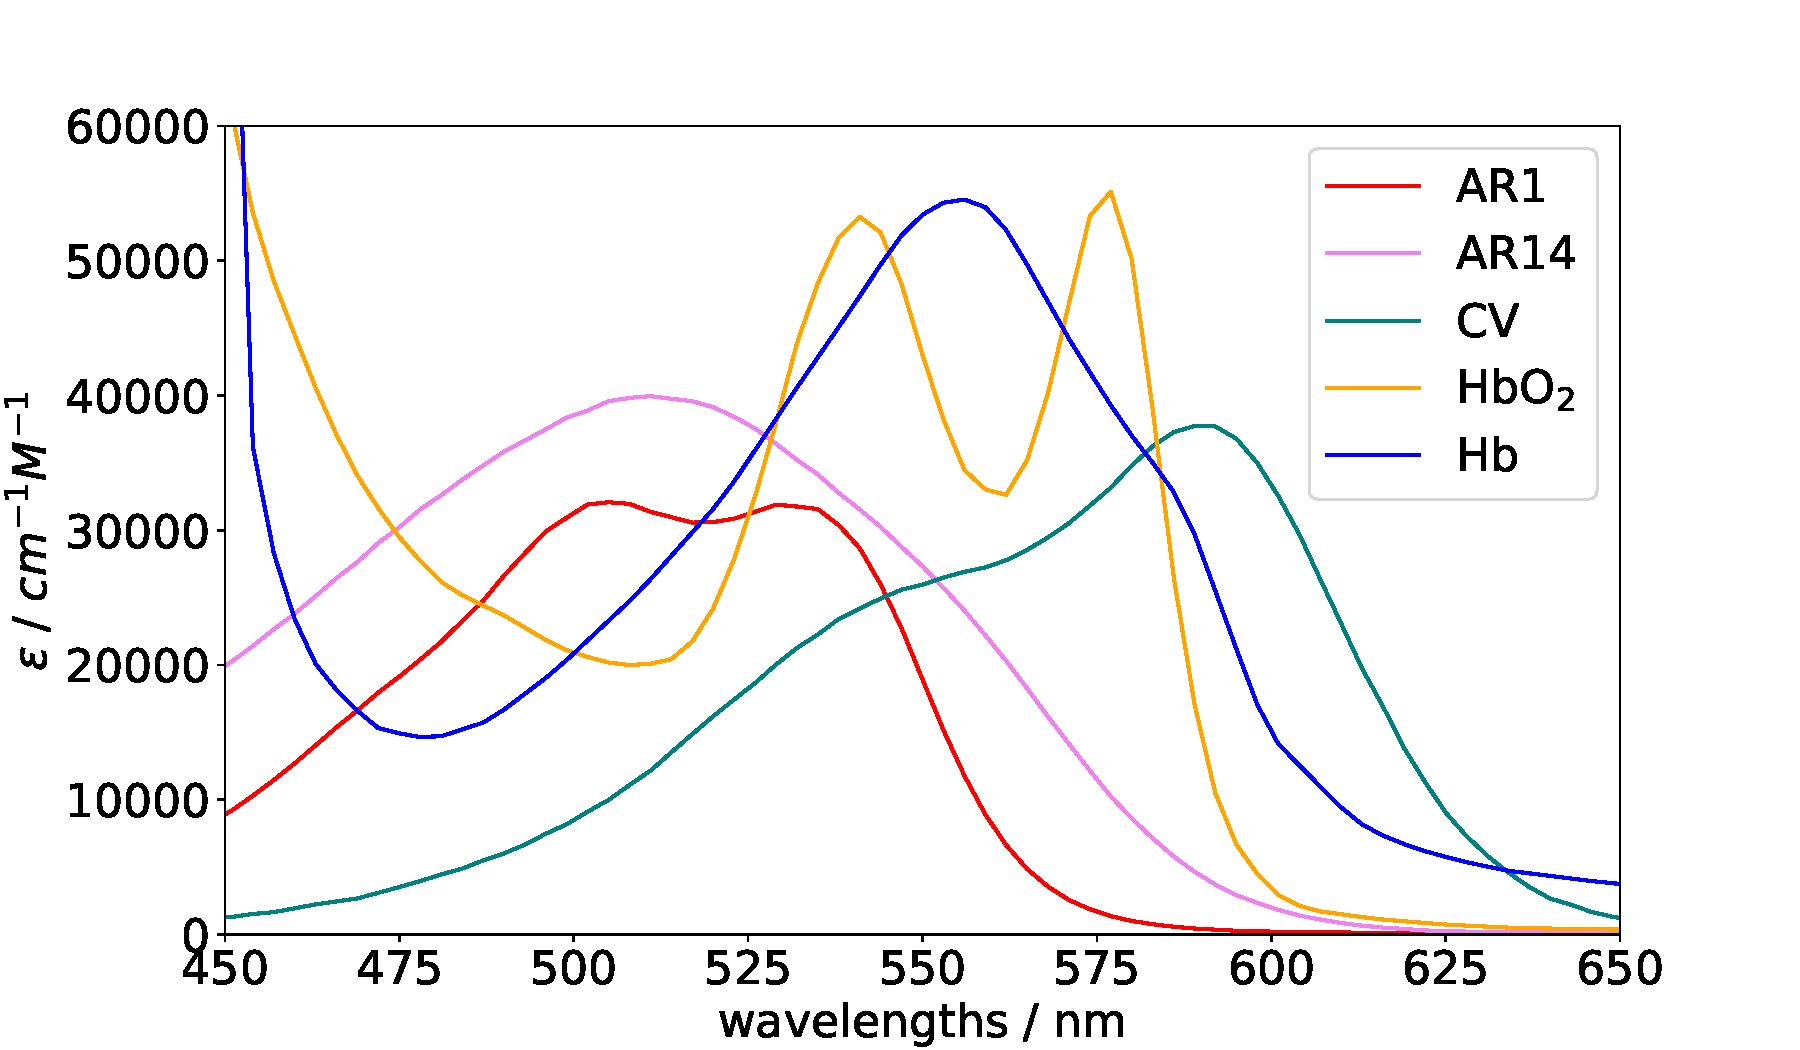
\includegraphics[width=\textwidth]{Figure_1a.pdf}
    %     \caption{}
    %     \label{fig:exteff}
    % \end{subfigure}
    % \hfill
    % \begin{subfigure}{0.44\textwidth}
    %     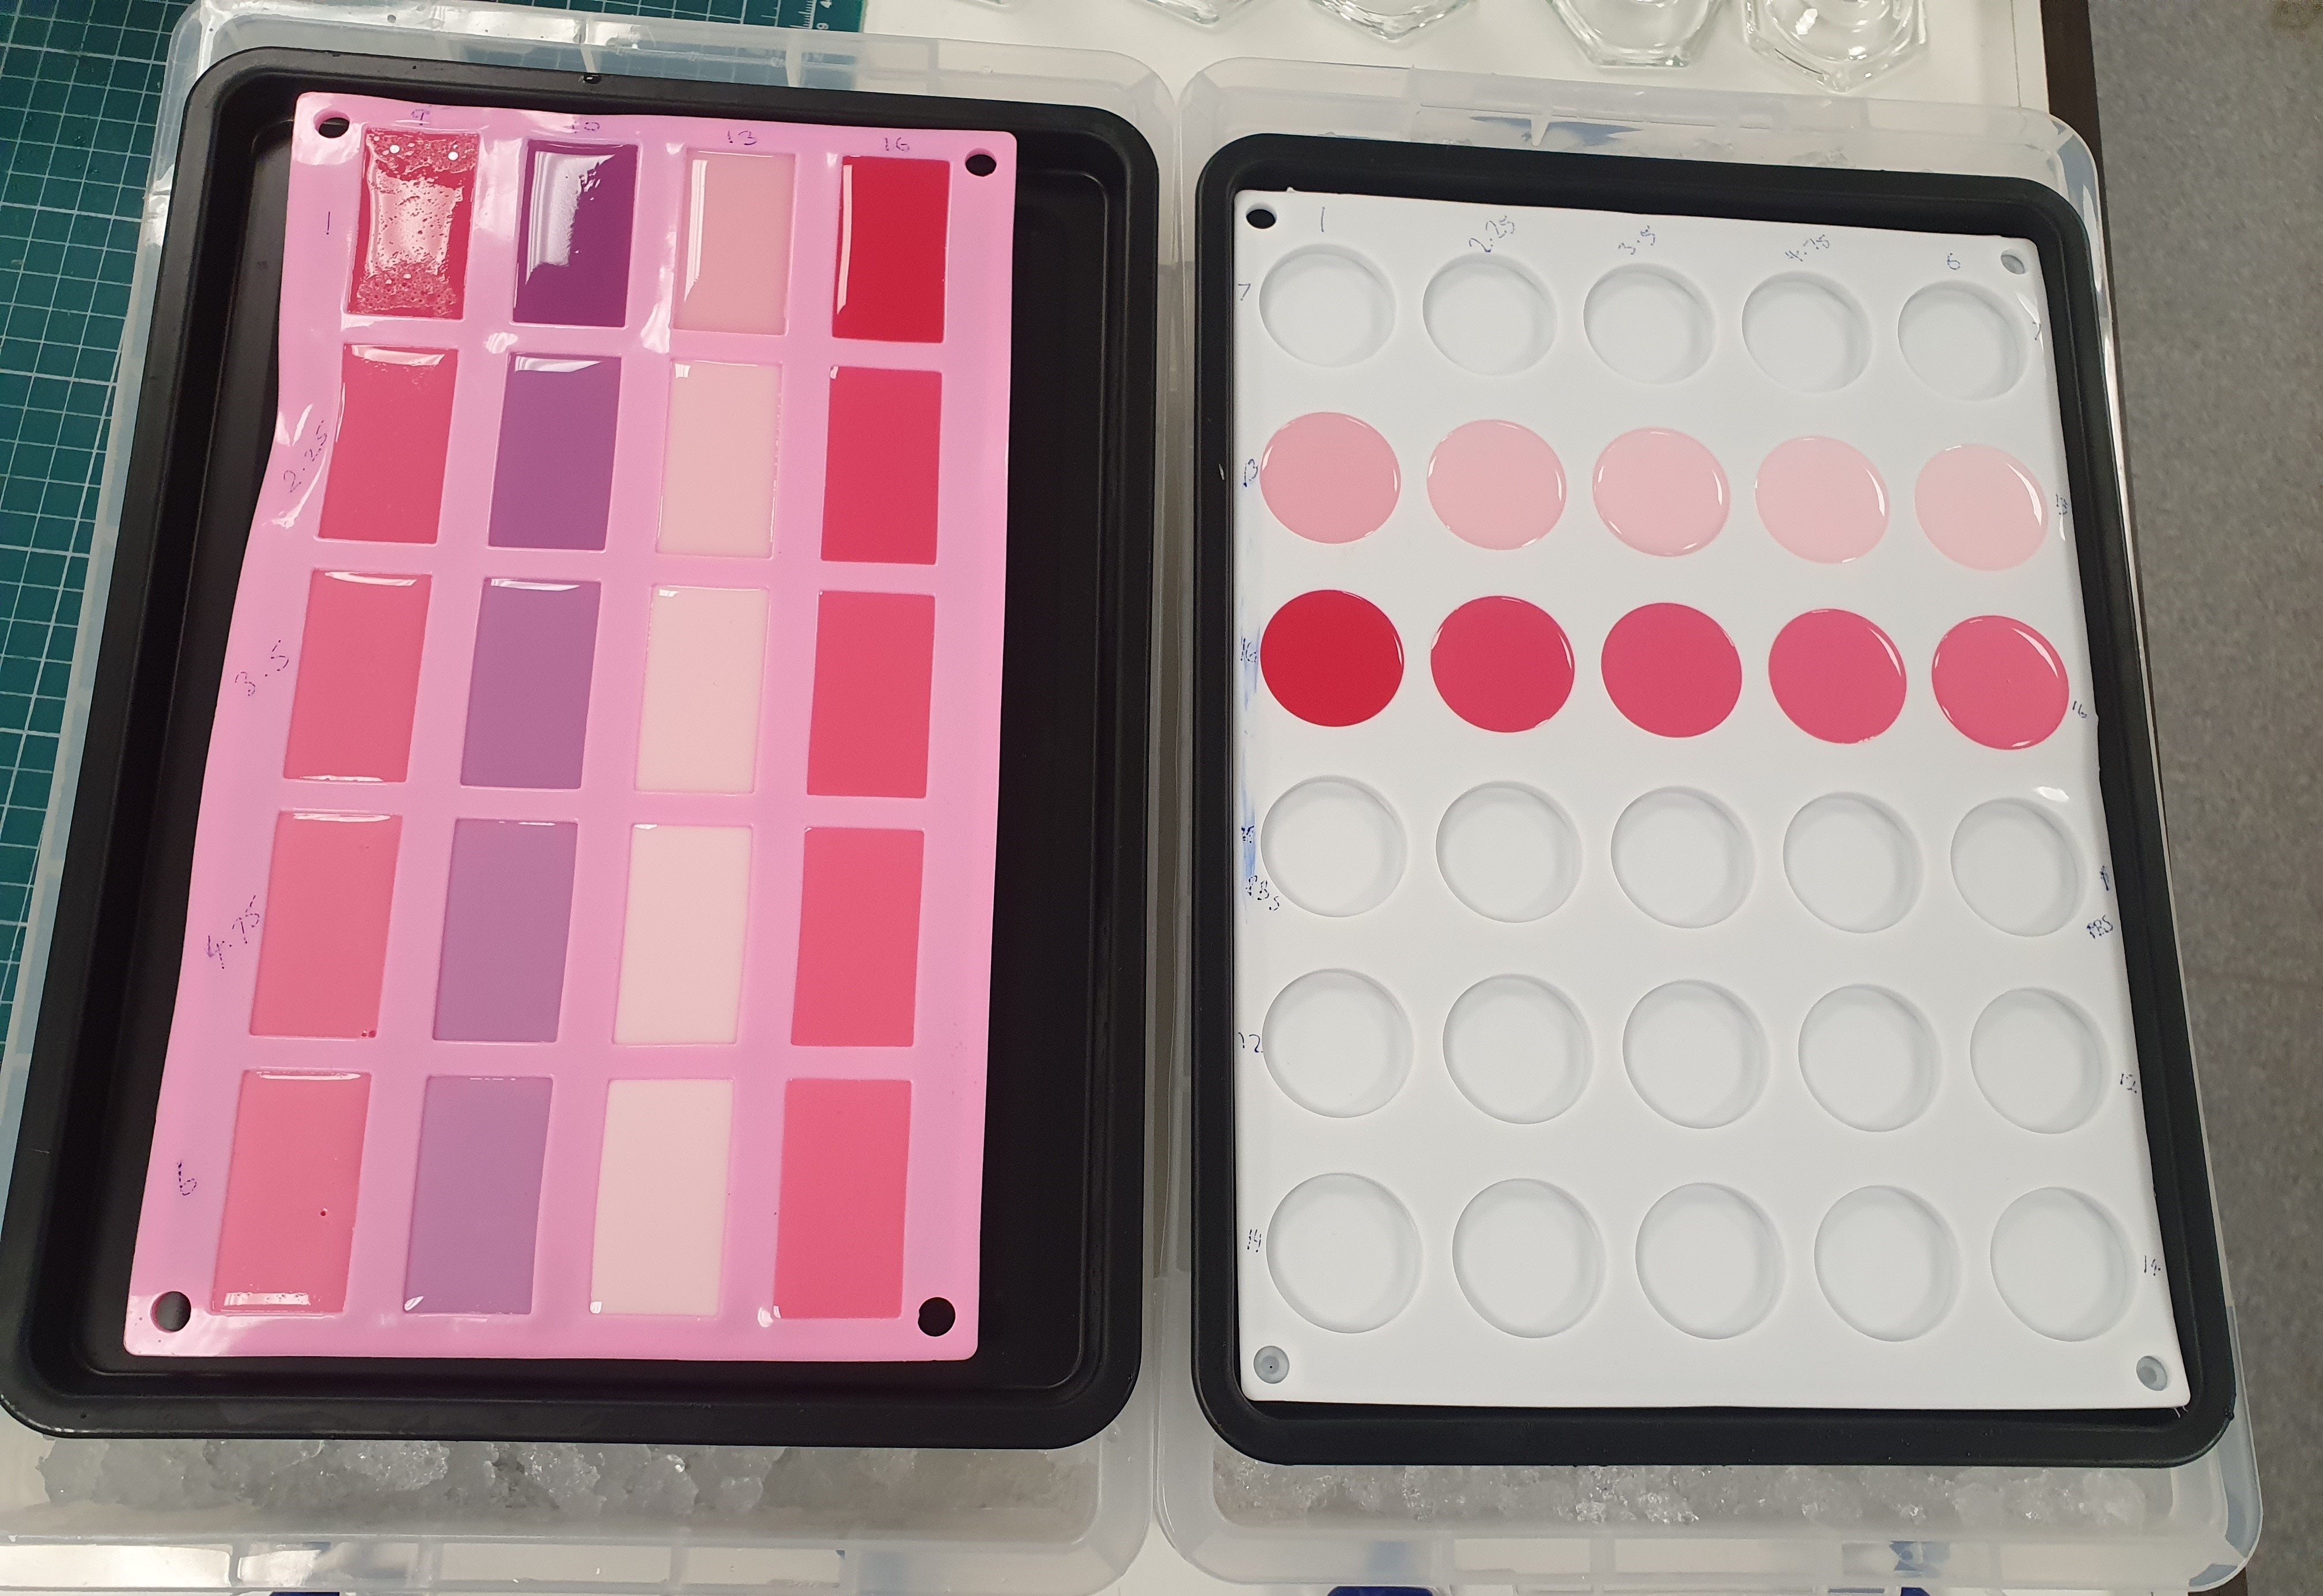
\includegraphics[width=\textwidth]{Figure_1b}
    %     \caption{}
    %     \label{fig:icebath}
    % \end{subfigure}
    % \begin{subfigure}{0.245\textwidth}
    %     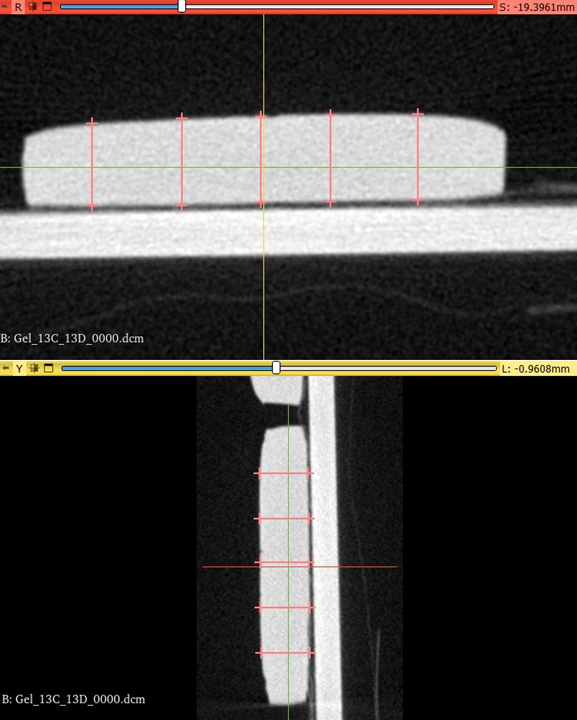
\includegraphics[width=\textwidth]{Figure_1c}
    %     \caption{}
    %     \label{fig:DICOM_Eg}
    % \end{subfigure}
    \caption{Figure regarding phantom development. 
    \textbf{(a)}
    Effective extinction coefficients of acid red 1 (AR1), acid red 14 (AR14), and crystal violet (CV) dyes 
    %\textcolor{red}{
    (used to synthesis gelatin-based phantoms)
    %}
    are displayed with the extinction coefficients of oxygenated (HbO$_2$) and deoxygenated haemoglobin (Hb) 
    %\textcolor{red}{
    (key tissue chromophores)
    %}
    .
    \textbf{(b)}
    Image of 1cm depth (left) and 5mm depth (right) phantoms setting in ice bath.
    %\textcolor{red}{
    \textbf{(c)}
    %}
    An example of a CT scan acquired for the purpose of measuring thickness of a tissue phantom is shown with
    %the
    10 digital measurements (mean=6.11mm)%
    %taken whose mean is calculated to be 6.11mm
    .}
    \label{fig:phantommethods}%\revref{1}{5}
\end{figure}

Phantoms are constructed with the ratios given in Table \ref{tb:phantomratios}, where each configuration is constructed with each intralipid concentration. 

\begin{table}[ht!]
    \centering
    \caption{Table displaying the 
    %\textcolor{red}{
    percentage of each 
    %}
    dye [acid red 1 (AR1), acid red 14 (AR14), crystal violet (CV)] a used for each dye configuration alongside the total dye scaled concentration in arbitrary units.}
    %\color{red}
    \begin{tabular}{|c|c|c|c|}
        \hline
        Total dye scaled concentration & \multicolumn{3}{|c|}{Dye 
        %\textcolor{red}{
        percentage (\%)
        %}
        } \\
        (arbitrary units) & AR1 & AR14 & CV \\
        \hline
        1 & 50 & 50 & 0 \\
        1 & 50 & 25 & 25 \\
        1 & 25 & 25 & 50 \\
        10 & 100 & 0 & 0 \\
        10 & 75 & 25 & 0 \\
        10 & 50 & 50 & 0 \\
        10 & 25 & 75 & 0 \\
        10 & 0 & 100 & 0 \\
        10 & 25 & 50 & 25 \\
        10 & 50 & 25 & 25 \\
        10 & 25 & 25 & 50 \\
        20 & 50 & 50 & 0 \\
        20 & 50 & 25 & 25 \\
        20 & 25 & 25 & 50 \\
        \hline
    \end{tabular}
    \label{tb:phantomratios} %\revref{1}{4}
\end{table}

\label{sec:methodsphantomsynthesis}
For each dye, stock solutions are made at double the required concentrations: 2x, 20x, and 40x in phosphate buffered saline (PBS, P4417, Merck, Germany) to allow for 1:1 dilution with intralipid as the final step. The stock concentrations are multiplied by a factor of $\frac{5}{3}$ for Acid Red 14 and $\frac{1}{2}$ for Crystal Violet to ensure similar absorbance impact. For each intralipid concentration, the stock solutions are made at double the required volume fractions: 2\% - 12\% to allow for 1:1 dilution with the dye solutions as the final step. The dye solutions combined in the correct ratios are heated to 45-50$^o$C with 12\% gelatin (i.e. double the required amount) until solvation. The solution is cooled to below 40$^o$C where 1\% formaldehyde (ie. double the quantity) is added and the solution is combined in equal quantities with the solution with double the desired intralipid concentration. This final solution now has the intended concentration of all constituents and is poured into a silicon mould in an ice bath, as seen in Figure \ref{fig:phantommethods}b, to ensure homogeneity in the final phantom by rapidly setting prior to any density separation. Once cooled to below 10$^o$C these are placed in a fridge at 4$^o$C to fully set for at least 7 days before measurement. 
% \begin{figure}
%     \centering
%     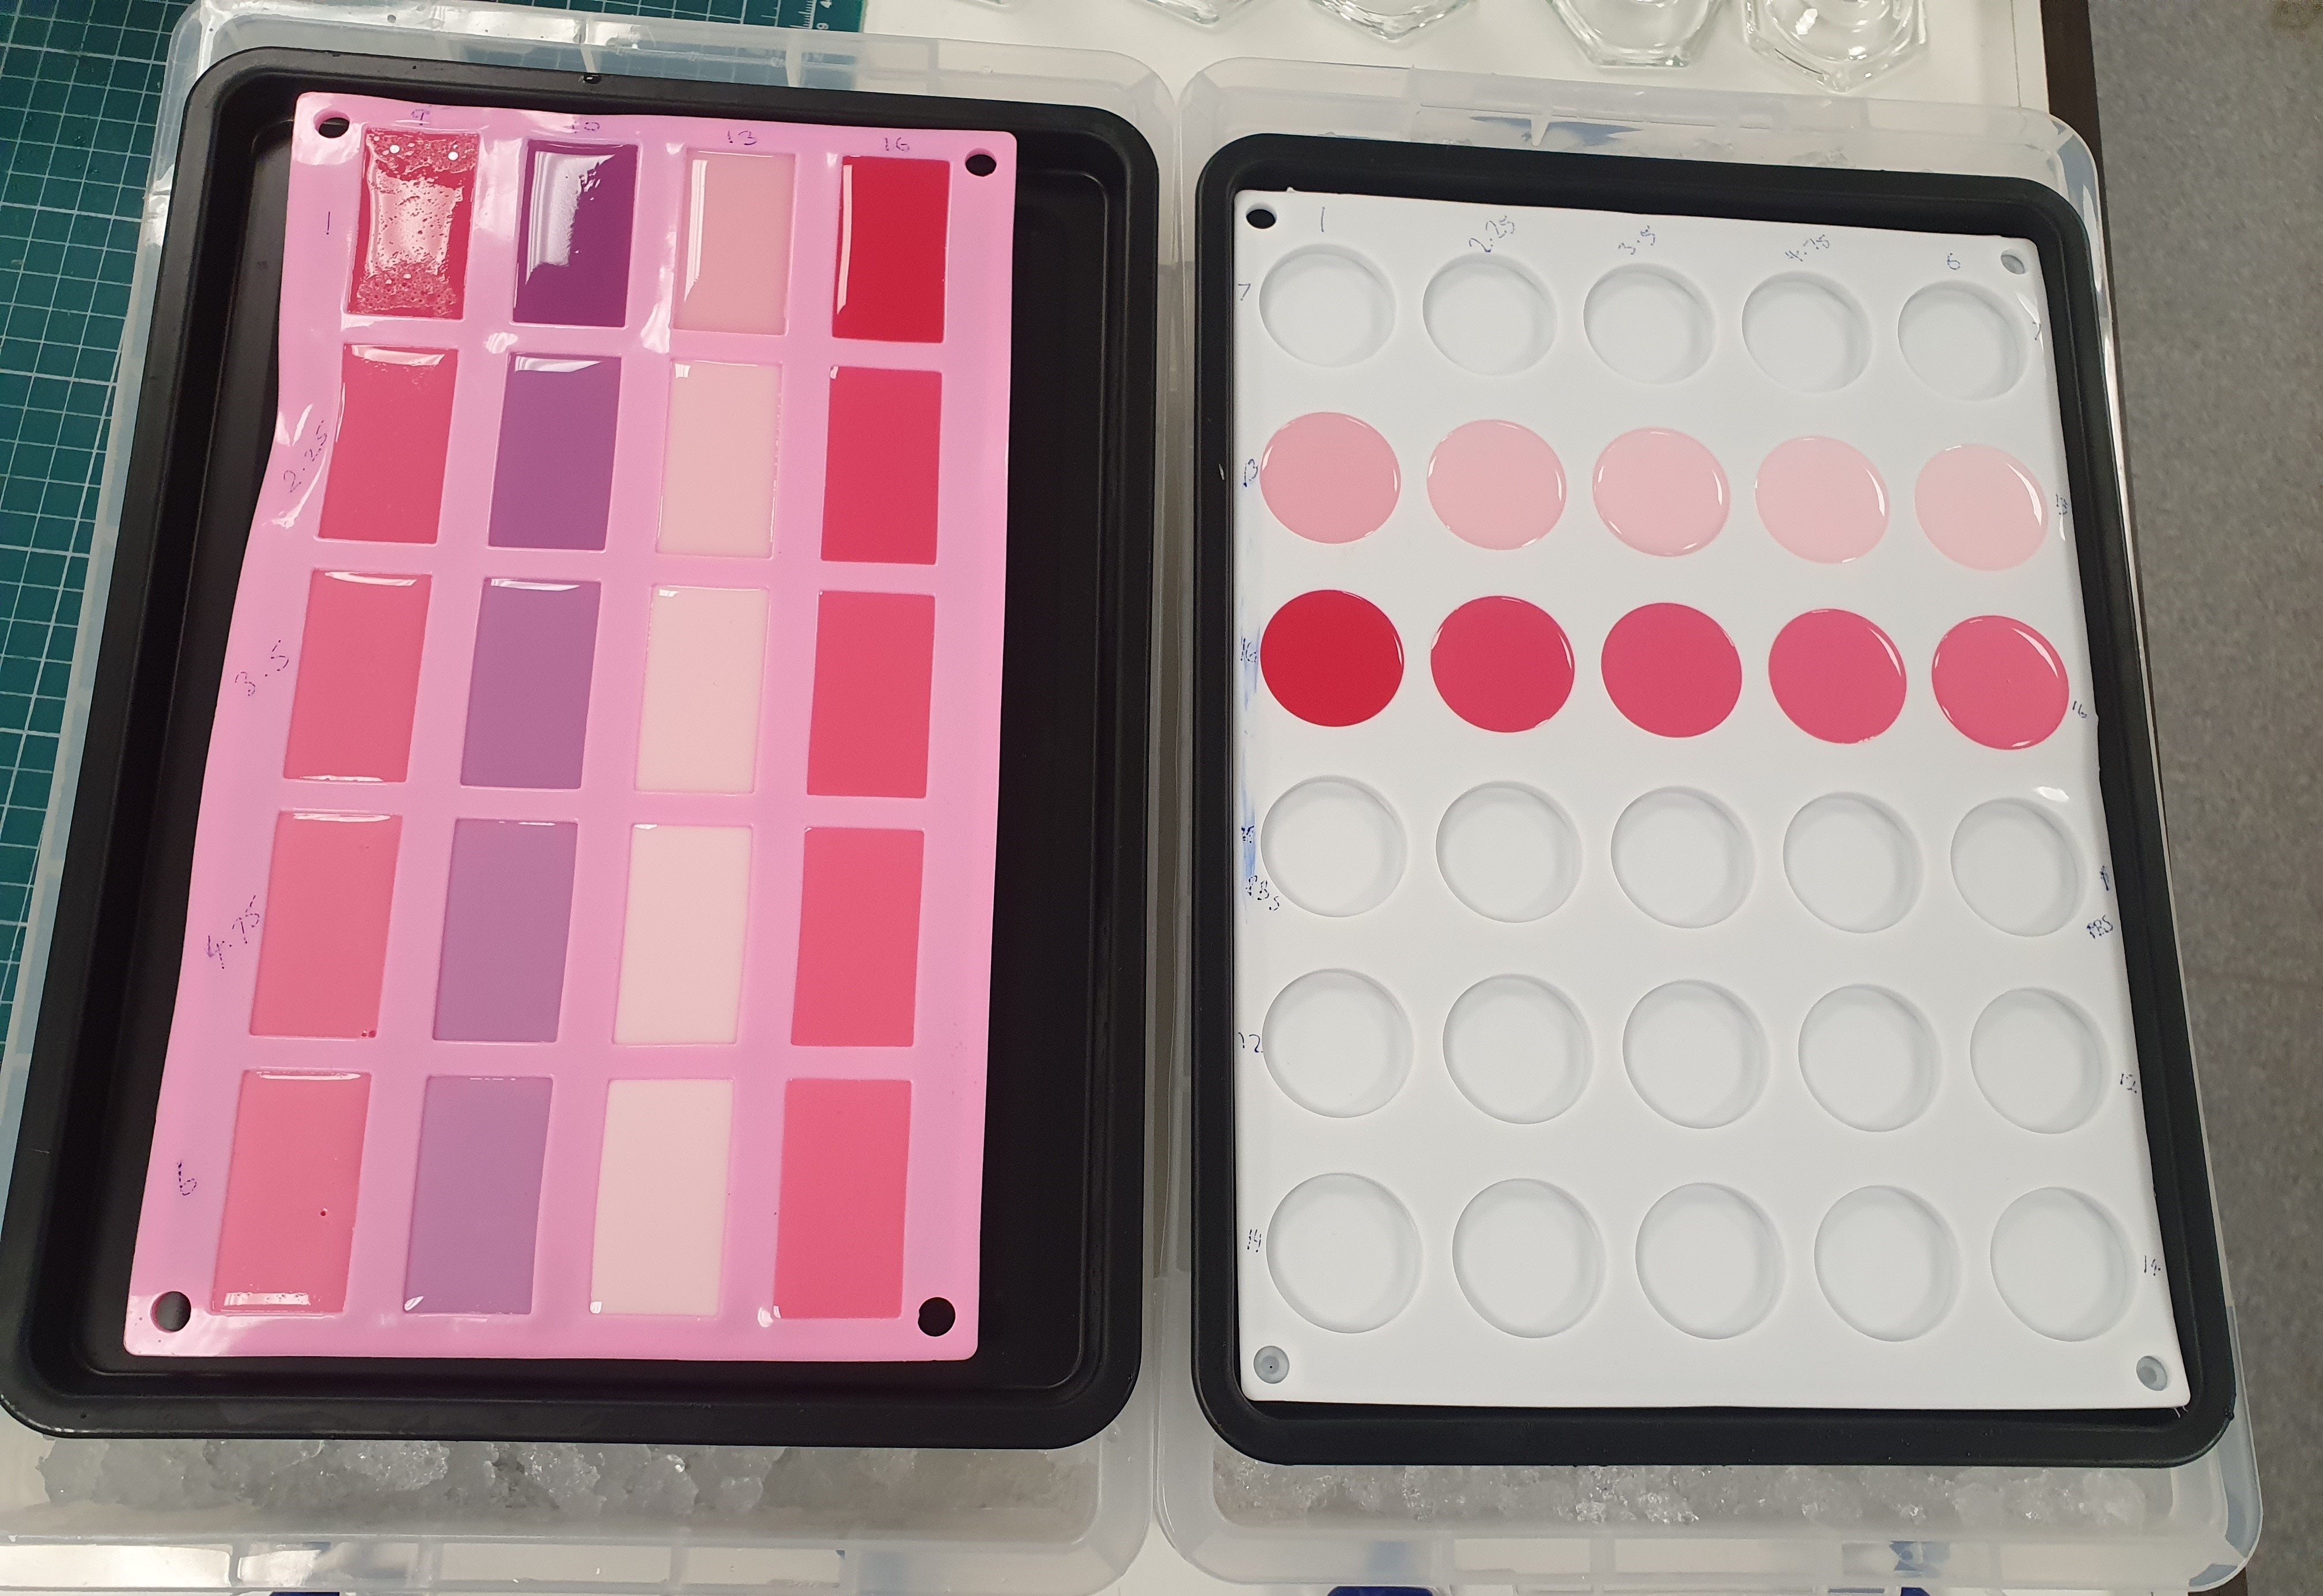
\includegraphics[width=0.6\textwidth]{Ice_bath_phantoms}
%     \caption{Image of 1cm depth (left) and 5mm depth (right) phantoms setting in ice bath.}
%  \label{fig:icebath}
% \end{figure}

Each dye solution is also combined with gelatin with a 0\% intralipid solution for absorbance measurements.
Additionally, each intralipid solution is combined with a gelatin solution with no dyes to allow analysis of scattering due to intralipid concentration.

Moulds with a depth of 1 cm are used to allow measurement of diffuse reflectance within a semi-infinite regime\cite{Zhang2014}.
MC simulations were used to confirm that this thickness was sufficient to be within the semi-infinite regime.
Some additional phantoms are constructed with a depth of 5 mm to allow for sufficient transmission for total transmittance measurements required for inverse adding doubling (IAD) analysis \cite{Prahl2017}. 
%to extract $\mu_a$ and $\mu_s'$ from total reflectance and diffuse transmittance measurements. 

% Justifications for all components chosen and their quantities can be found in Page \pageref{sec:methodsphantomcomposition}.

\paragraph{Spectral measurements}\label{sec:methodsphantommeasure1}
Measurements of these phantoms are taken using a PerkinElmer Lambda 750s spectrophotometer. This dual-beam integrating sphere spectrophotometer allows for precise and accurate measurements of diffuse reflectance, total reflectance, total transmittance, and absorbance. Absorbance for each dye solution and pure dye gelatin phantom is measured with either PBS or pure gelatin as a reference respectively. The pure gelatin absorbance is also measured. 
All 1cm phantoms are used for diffuse reflectance measurements. A subset of these are also made into 5mm phantoms alongside pure intralipid gelatin 5mm phantoms, which are measured for total reflectance and total transmittance. 
All configurations are depicted for our system in Figure \ref{fig:spectrophotometer}. 
\begin{figure}[t!]
    \centering
    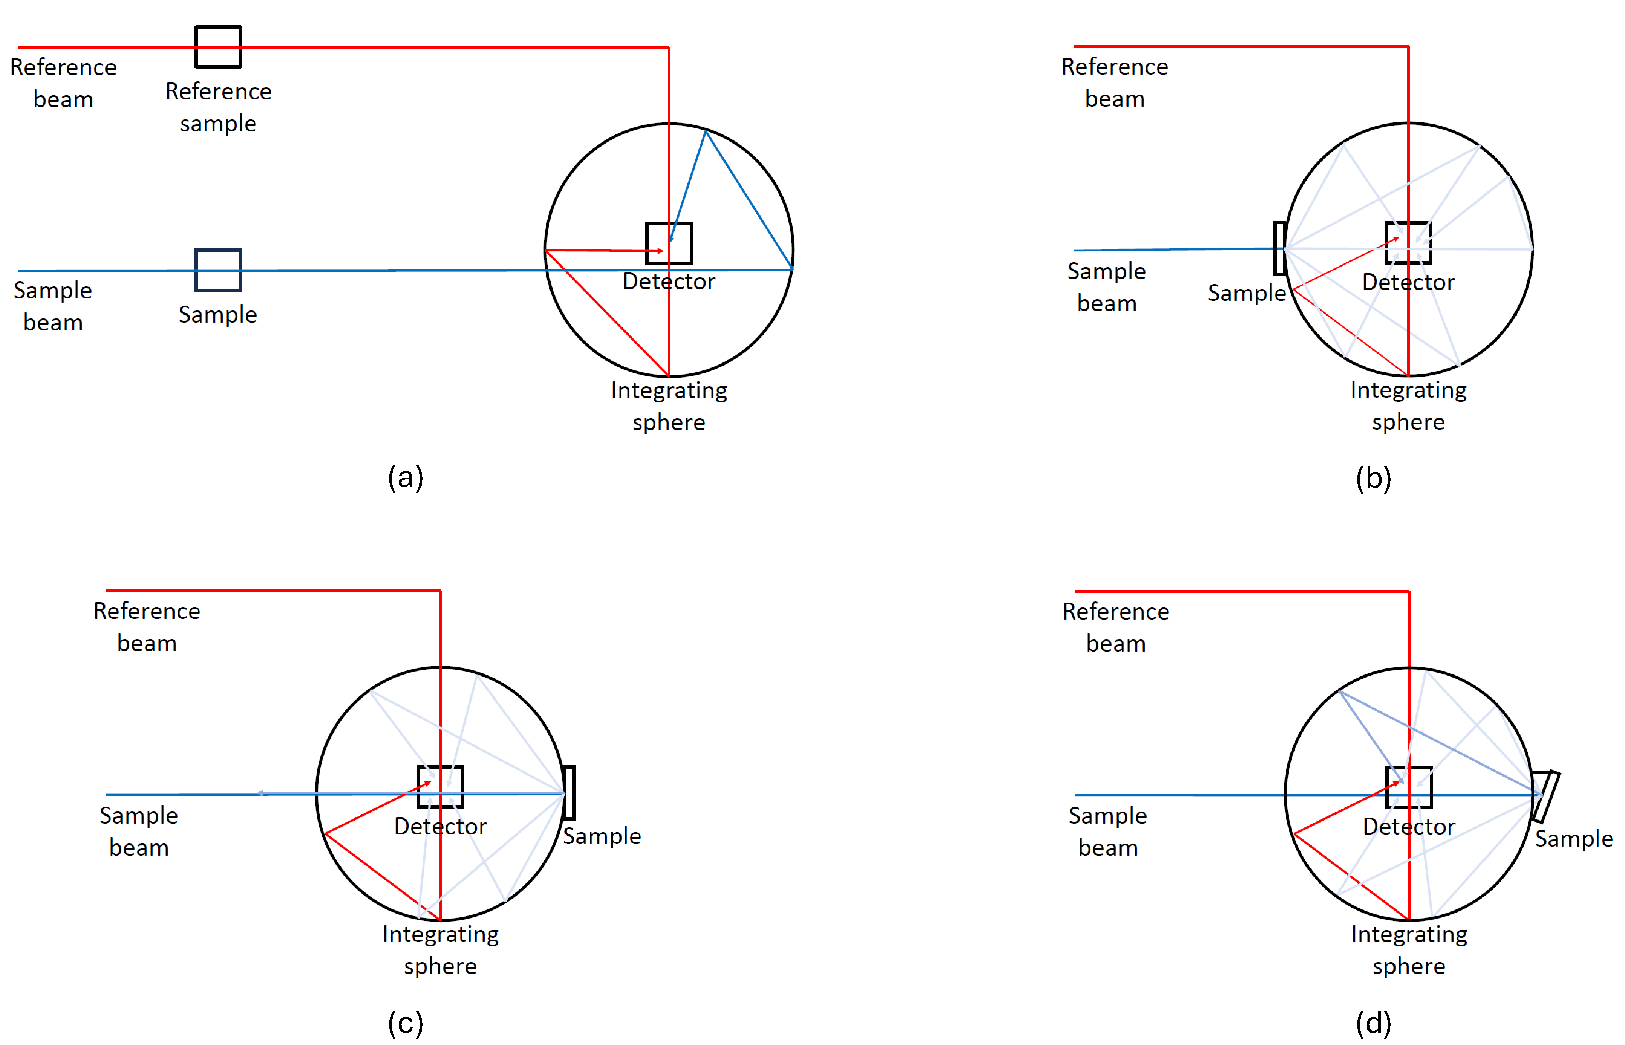
\includegraphics[width=\textwidth]{Figure_2.pdf}
    % \begin{subfigure}{0.47\textwidth}
    %     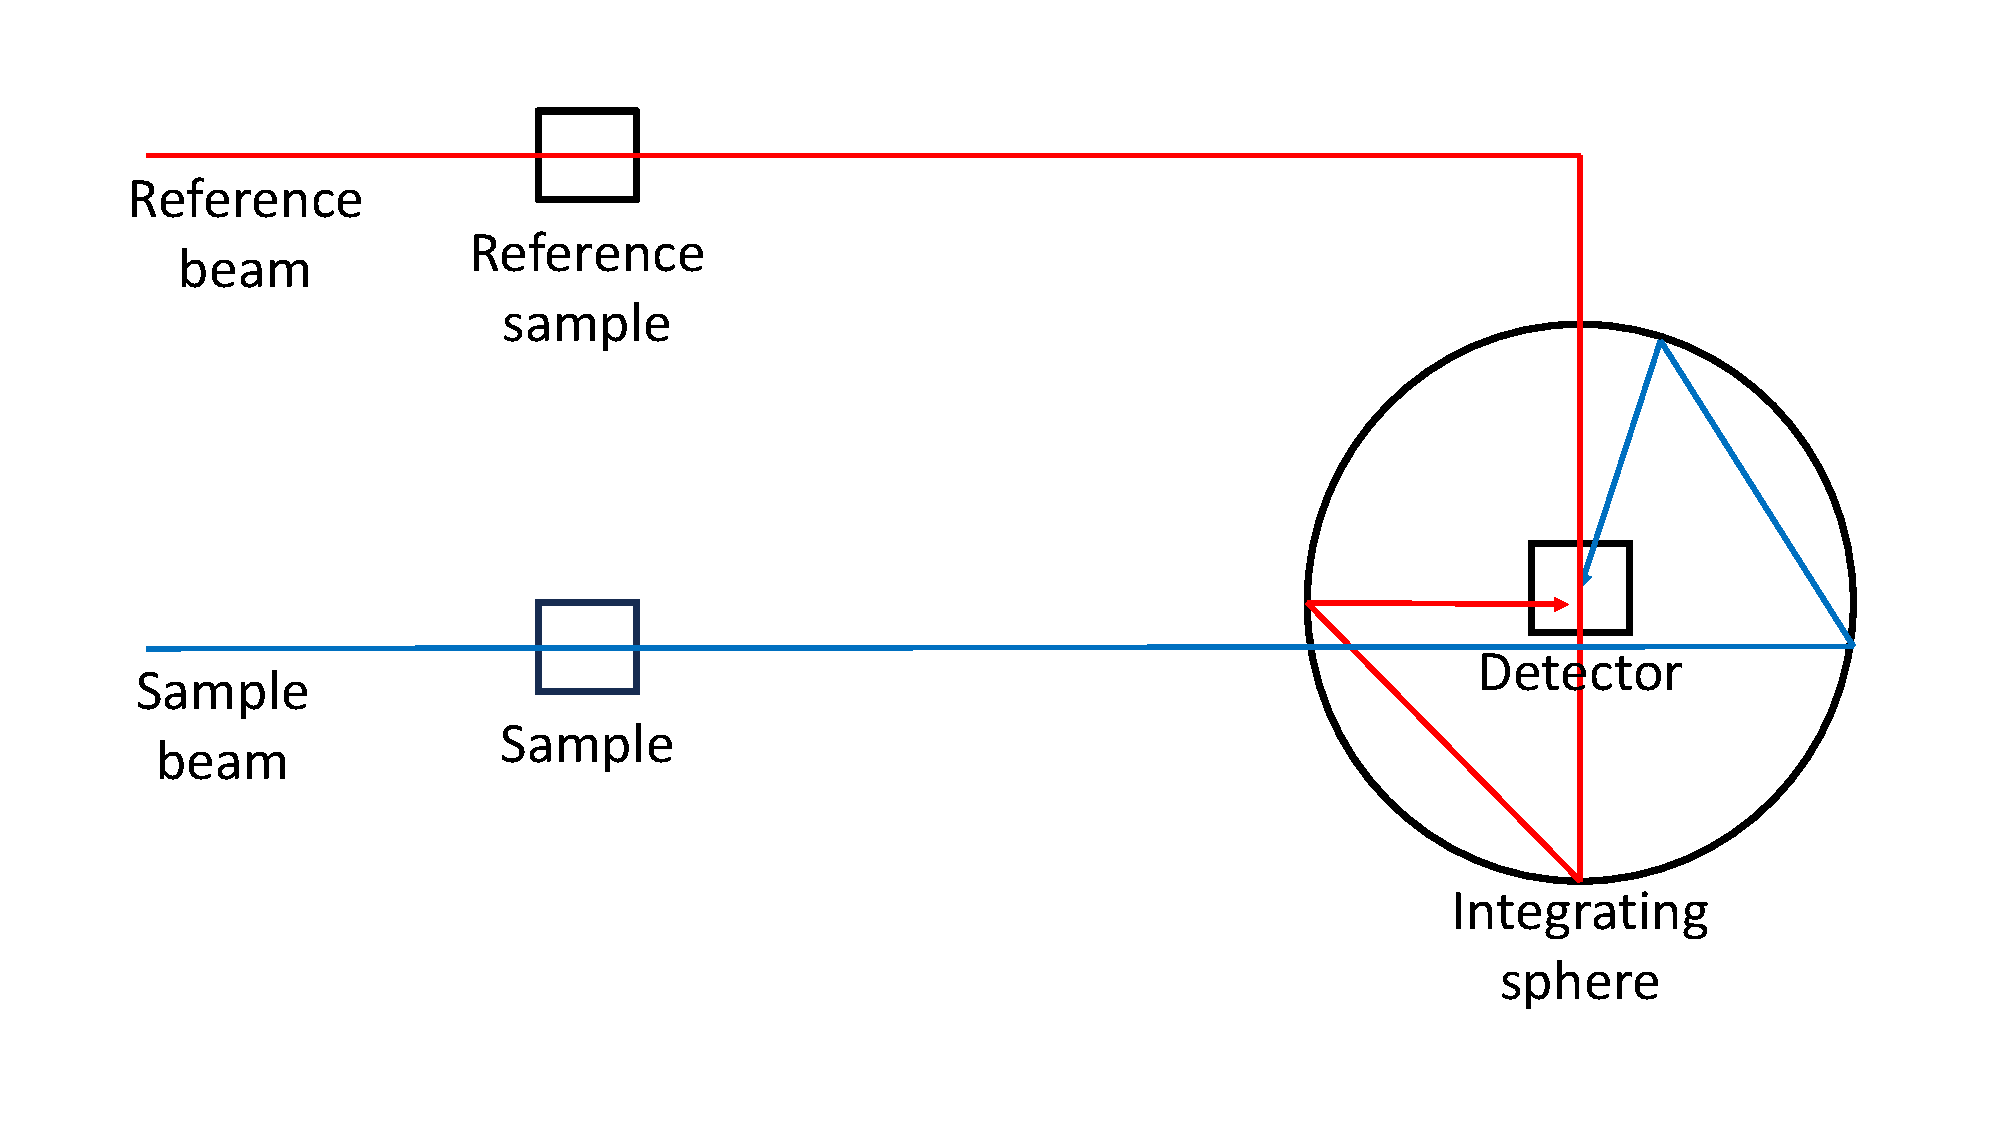
\includegraphics[width=\textwidth]{Figure_2a.pdf}
    %     \caption{}
    %     \label{fig:spectrophotometer_abs}
    % \end{subfigure}
    % \begin{subfigure}{0.47\textwidth}
    %     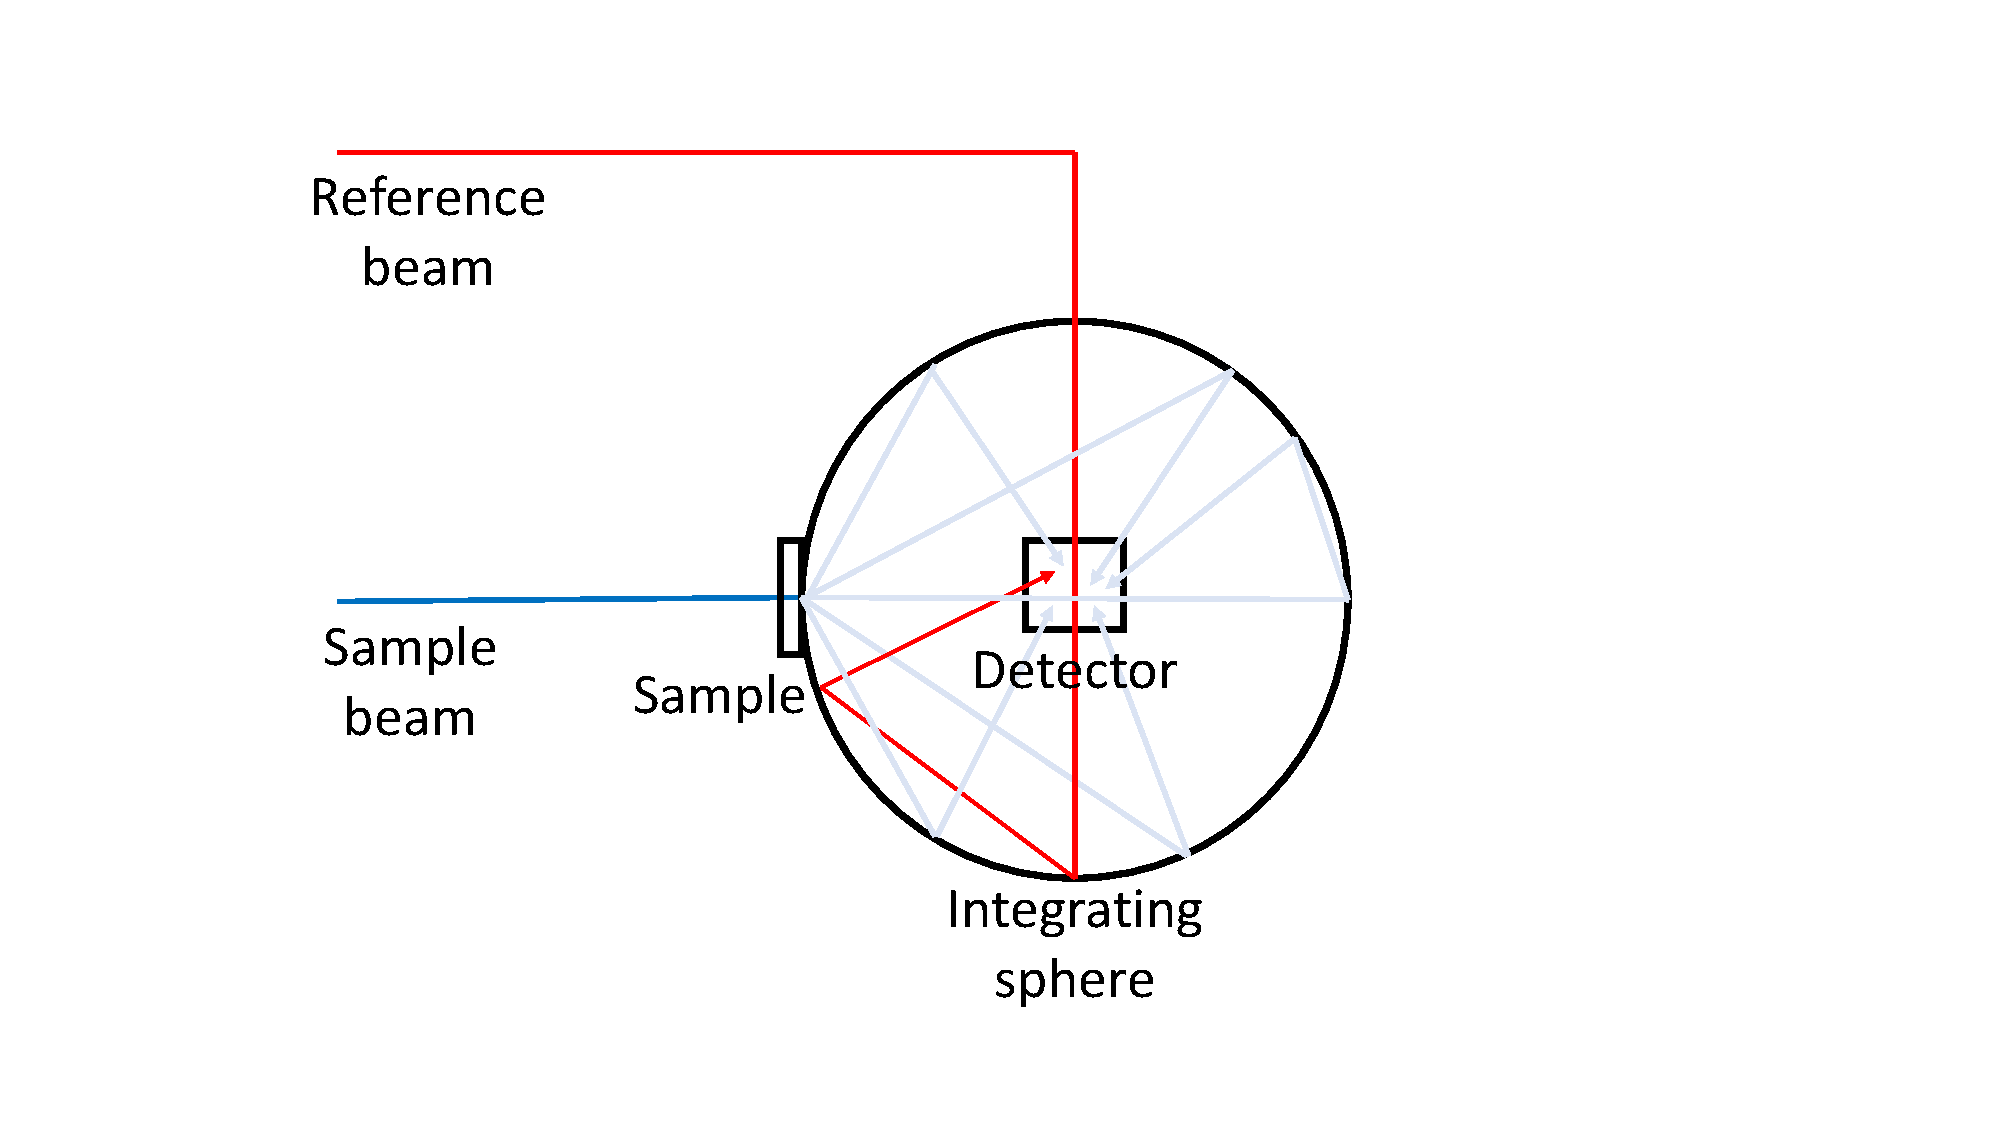
\includegraphics[width=\textwidth]{Figure_2b.pdf}
    %     \caption{}
    %     \label{fig:spectrophotometer_dT}
    % \end{subfigure}
    % \hfill
    % \begin{subfigure}{0.47\textwidth}
    %     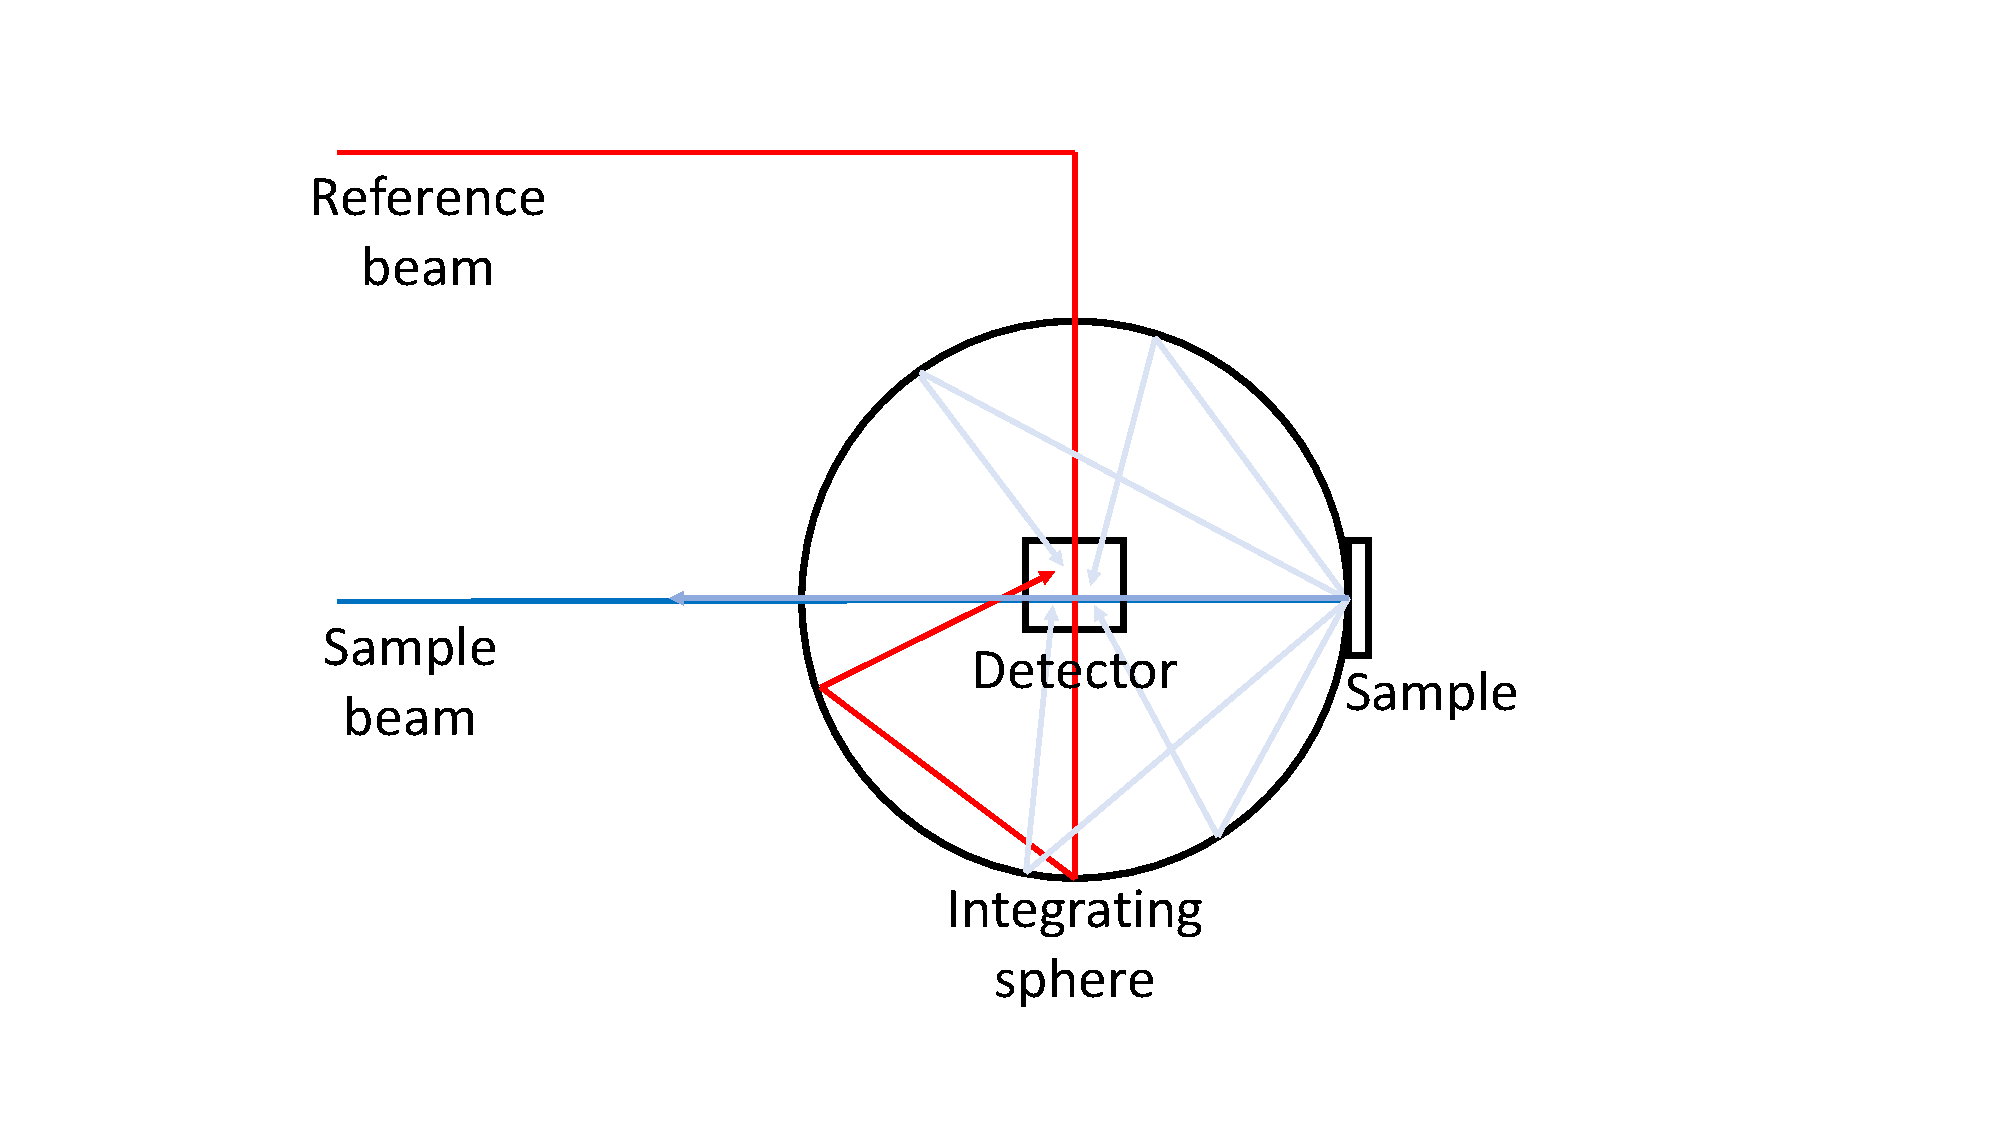
\includegraphics[width=\textwidth]{Figure_2c.pdf}
    %     \caption{}
    %     \label{fig:spectrophotometer_dR}
    % \end{subfigure}
    % \begin{subfigure}{0.47\textwidth}
    %     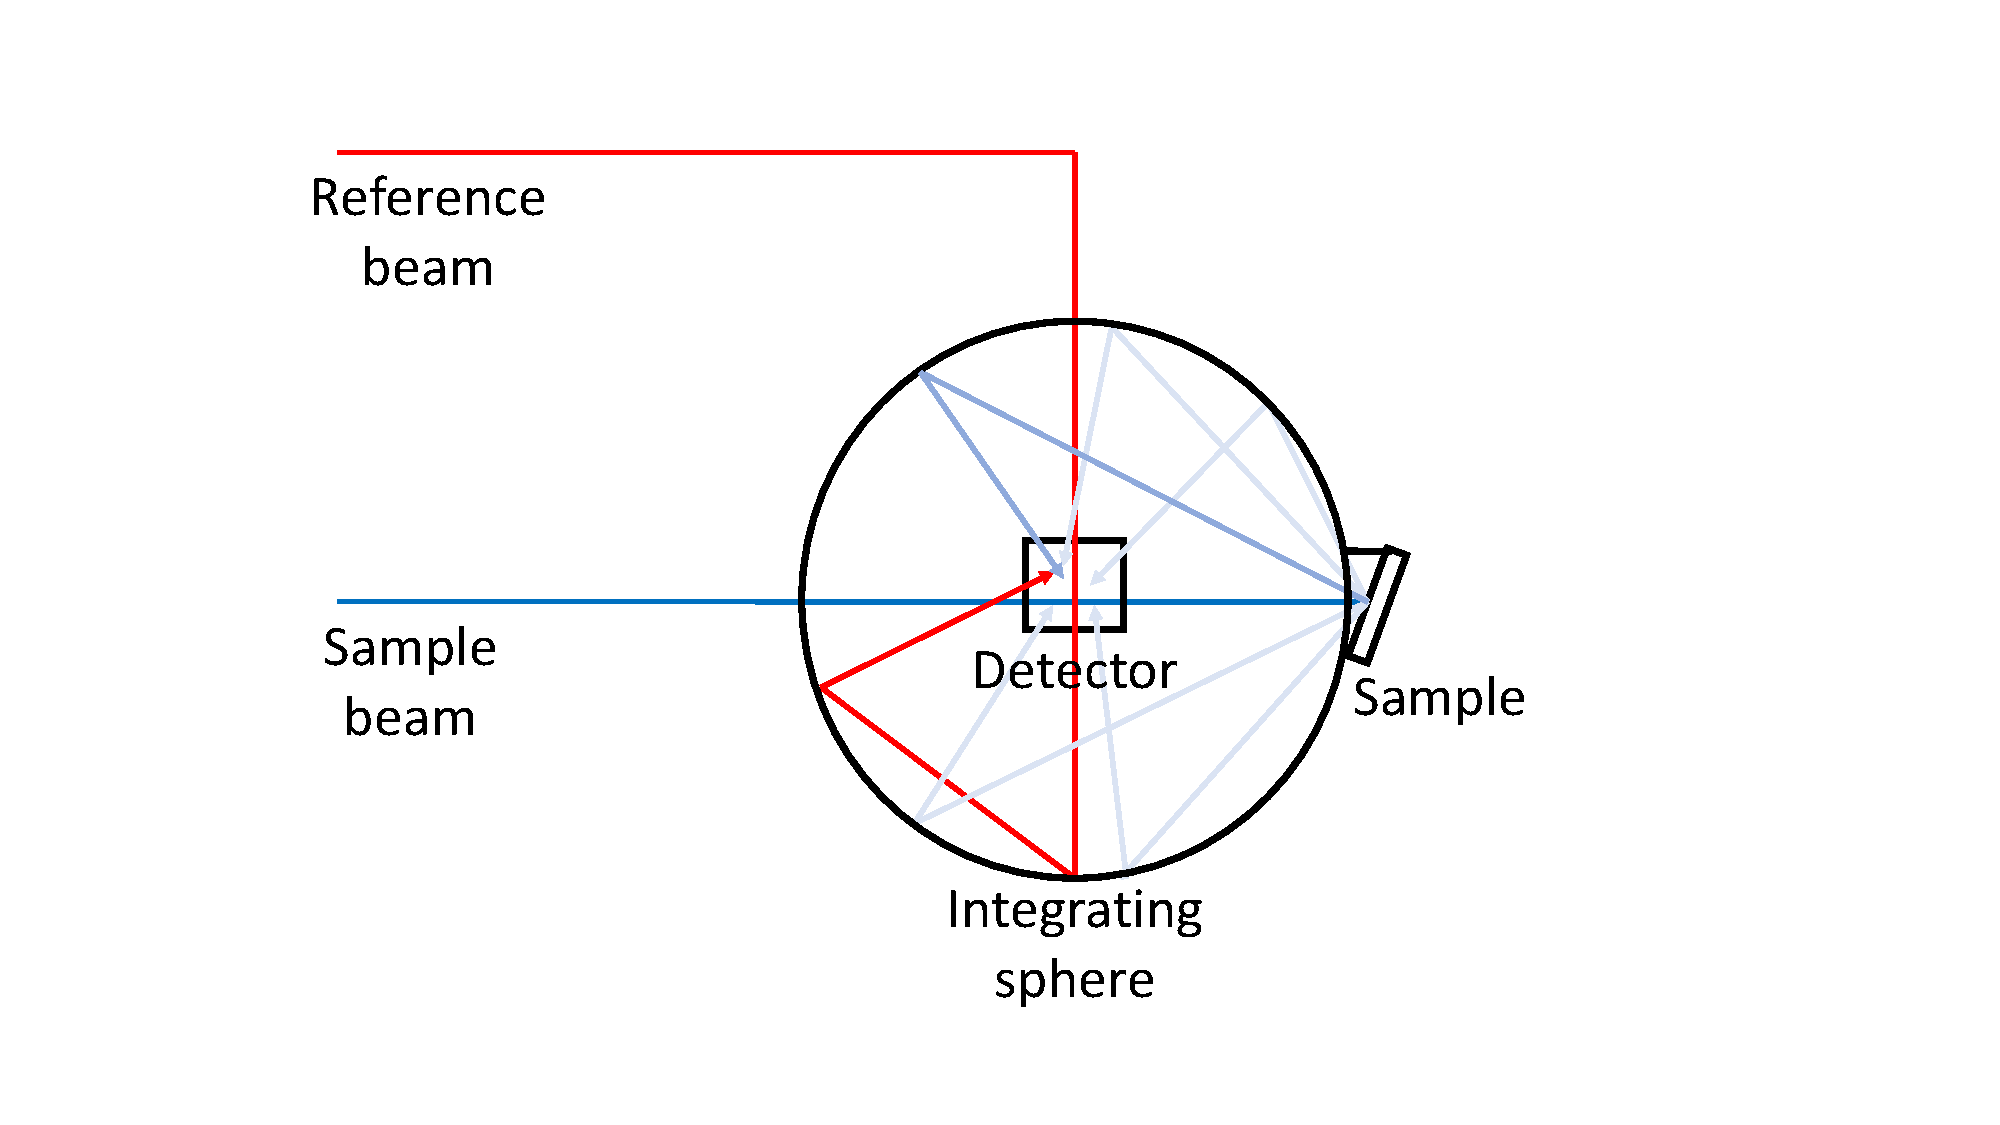
\includegraphics[width=\textwidth]{Figure_2d.pdf}
    %     \caption{}
    %     \label{fig:spectrophotometer_tR}
    % \end{subfigure}
    \caption{Depictions of measurement set-up for spectrophotometer measurements of gelatin based tissue phantoms of absorbance (a), total transmittance (b), diffuse reflectance (c), and total reflectance (d) where an 8$^o$ wedge is used to ensure the specular reflectance is also included.}
    \label{fig:spectrophotometer}
\end{figure}
%\FloatBarrier

\paragraph{Inverse adding doubling (IAD)}\label{sec:methodsphantommeasure2}
IAD is used to obtain $\mu_a(\lambda)$ and $\mu_s'(\lambda)$ from total reflectance and total transmittance measurements \cite{Prahl2017}. We use this with the dual beam spectrophotometer setting and an incidence angle of 8$^o$ as per the experimental set-up in Figure~\ref{fig:spectrophotometer}d, with $g$ fixed to 0.8 for all calculations since it was found not to change the results. Since the outputted optical properties can contain a significant number of wavelengths without convergence, a Mie scattering curve is fitted to the output $\mu_s'(\lambda)$ and a second stage of IAD is run with the $\mu_s'(\lambda)$ fixed to this spectrum.
This returns outputs which are very similar but removing noise or errors.
Further details on this two-stage IAD fitting approach can be found in previous work\cite{Xie2021}. 

In order to obtain accurate optical properties from IAD a highly accurate sample depth must be provided. 
%\textcolor{red}{
The standard measurement technique using dial calipers is not suitable in this case due to the highly compressible nature of the gelatin-based phantoms.
A non-contact measurement method is therefore chosen. A
%}
CT scan is taken of each phantom using a Small Animal Radiotherapy System (SmART+, precision X-ray). A mean of 10 digital measurements is used for each phantom and an example of these measurements is shown in Figure \ref{fig:phantommethods}c.
% \begin{figure}
%     \centering
%     \includegraphics[width=0.5\textwidth]{DICOM_Eg}
%     \caption{An example of a CT scan of a tissue phantom and 10 digital measurements taken of the phantom thickness.}
%      \label{fig:DICOM_Eg}
% \end{figure}

Finally, a commercial calibrated phantom (BioPixS) with validated ground truth optical properties at three wavelengths is used to confirm that our output $\mu_a(\lambda)$ and $\mu_s'(\lambda)$ are correct. We highlight that only the single-stage IAD algorithm can be used here as a Mie scattering curve does not accurately represent the scattering of this sample. The BioPixS phantom is measured on three days to demonstrate the accuracy and reproducibility of IAD-outputted optical parameters.

\paragraph{Modelling tissue phantom optical properties}\label{sec:methodphantommodel}
The $\mu_a(\lambda)$ of the two-dye configuration phantoms can be modelled as in Equation \eqref{eq:phantommua} where the background spectrum is determined by measuring the absorption of pure gelatin solution, whereas the scattering is modelled based on the intralipid concentration according to trends determined using IAD. 
\begin{equation}
    \mu_{a}(\lambda) = 8\times10^{-6}c_{tot}\ln(10)[AR1 \epsilon_{AR1, eff}(\lambda) + 
    %\textcolor{red}{
    (1 - AR1)
    %}
    \epsilon_{AR14, eff}(\lambda)] + \mu_{a, background}(\lambda)
    \label{eq:phantommua} %\revref{2}{2}
\end{equation}
In this equation $c_{tot}$ is the total concentration of dye independent of dye identity, $AR1$ and 
%\textcolor{red}{
$AR14 (=1-AR1)$
%}\revref{2}{2}
are the relative ratios of each dye, $\epsilon_{AR1, eff}(\lambda)$ and $\epsilon_{AR14, eff}(\lambda)$ are the effective extinction coefficients of each dye, and  $\mu_{a, background}(\lambda)$ is the measured background absorbance from gelatin. This can be adapted to a three-dye configuration as follows: 
\begin{equation}
    \mu_{a}(\lambda) = 8\times10^{-6}c_{tot}\ln(10)[AR1 \epsilon_{AR1, eff}(\lambda) + AR14\epsilon_{AR14, eff}(\lambda) + (1 - AR1 - AR14)\epsilon_{CV, eff}(\lambda)] + \mu_{a, background}(\lambda)
    \label{eq:phantommua3}
\end{equation}
Where 
%\textcolor{red}{
$CV (=1-AR1-AR14) $
%}\revref{2}{2}
is the relative ratio of crystal violet and $\epsilon_{CV, eff}(\lambda)$ is the effective extinction coefficient of this dye.

\subsection{Evaluation of model performance}\label{sec:methodevaluate}
In this work, the above models are evaluated against spectra with known ground truth. These reference spectra are either found by MC simulation or measurement of controlled phantoms, however the evaluation of each is broadly the same. The forward models are evaluated in terms of the fit of their predicted spectra, and the inverse problem solutions (parametric fits) are investigated in terms of the quality of parameter extraction. 

Diffuse reflectance spectra can be predicted by inputting ground truth values into each forward tissue model and compared to corresponding reference (%\textcolor{red}{
MC/measured%}\revref{2}{3}
) spectra. The Normalised Root Mean Squared Error ($NRMSE$), defined in Equation \eqref{eq:NRMSE}, is calculated to quantitatively evaluate the similarity between the reflectance predicted by the forward model and the associated reference (
%\textcolor{red}{
MC/measured%}\revref{2}{3}
) reflectances. In the context of this work the wavelength ranges considered for this metric correspond to those ranges used for fitting the inverse models.
\begin{equation}
    NRMSE = \frac{\sqrt{\frac{1}{\Lambda}\sum_{\lambda}^{\Lambda}\left(s_{\lambda} - r_{\lambda}\right)^2}}{\sqrt{\frac{1}{\Lambda}\sum_{\lambda}^{\Lambda} r^2_{\lambda}}}
    \label{eq:NRMSE}
\end{equation}
Here the modelled spectrum $s_{\lambda}$ at any given wavelength $\lambda$ is evaluated against the intensity at the same wavelength in the reference (
%\textcolor{red}{
MC/measured
%}\revref{2}{3}
) spectrum $r_{\lambda}$ using the normalized root mean squared error ($NRMSE$) calculated across all $\Lambda$ wavelengths. These forward model reflectance spectra are also plotted against the reference (
%\textcolor{red}{
MC/measured
%}\revref{2}{3}
) reflectance spectra and a regression line calculated. This is evaluated using the Pearson correlation coefficient ($r$) and the p-value ($p$) for a hypothesis test with the null hypothesis that there is no correlation. Using a 95\% confidence interval, significant $p$ is less than 0.05, whereas a strong correlation is demonstrated by $r$ close to 1.  This gives an indication of similarity in shape, while disregarding offsets.

The inverse problem solutions can also be evaluated by determining how well they recover the ground truth input parameters using a non-linear least squares fitting approach (using SciPy v1.10.0 \href{https://docs.scipy.org/doc/scipy/reference/generated/scipy.optimize.least_squares.html}{\texttt{scipy.optimize.least\_squares}} function). The cost function for this is shown in Equation \eqref{eq:leastsquares} where $R(\lambda)$ is the reference (
%\textcolor{red}{
MC/measured
%}\revref{2}{3}
) spectrum and $M$ is the forward model function. This equation is modified to fit the parameters used to calculate $\mu_a(\lambda)$ and $\mu_s'(\lambda)$ directly.
\begin{equation}
    argmin_{\mu_{a}(\lambda), \mu_{s}'(\lambda)} \sum (R - M(\mu_{a}(\lambda), \mu_s'(\lambda))^2
    \label{eq:leastsquares}
\end{equation}

All models are fitted by only considering wavelengths up to 600nm as this is the region the Yudovsky model has been shown to be effective by the authors\cite{Yudovsky2011a}.
When fitting to measured phantom spectra, only wavelengths up to 575nm are considered due to the forward model predicted spectra being highly unreliable after this point for all three models as discussed in Section \ref{sec:resultsPhantoms}. The quality of parameter recovery is examined by calculating the correlation between the fitted and ground truth parameters (using SciPy v1.10.0 \href{https://docs.scipy.org/doc/scipy/reference/generated/scipy.stats.linregress.html}{\texttt{scipy.stats.linregress}} function). This is evaluated with the Pearson correlation coefficient ($r$) and the p-value ($p$) as above. The quality of parameter recovery is also evaluated using absolute percentage errors ($APE$) as given by Equation \eqref{eq:percenterr} where $e$ is the extracted parameter and $g$ is the ground truth parameter. The median and inter-quartile range of these parameters are presented for each dataset. 
\begin{equation}
    APE = |\frac{e - g}{g}| \times 100 
    \label{eq:percenterr}
\end{equation}

These evaluation methods can be done for quantitative or relative spectra. Here relative spectra are defined as mean normalised spectra. This allows parameters to be extracted considering the shape of the spectrum but without considering absolute intensity. This is investigated as it is simpler to capture relative data in clinical environments \cite{Bahl2023}.

\section{Results}\label{sec:results}
\subsection{Monte Carlo}\label{sec:resultsMC}
Each model has hyperparameters which are fitted to MC datasets for refractive indices 1.33, 1.35, and 1.44. These are listed in 
%\textcolor{red}{
Table \ref{tb:fittedmodelparams}
%}\revref{2}{4}
alongside any literature hyperparameters \cite{Jacques1999, Yudovsky2009}.
\begin{table}[htb!]
    \centering
    \caption{Table displaying single layer model hyperparameters fitted to MC datasets of each refractive index (black) with available literature values (blue).}
    \begin{tabular}{|cc|cc|c|cc|}
        \hline
        \multirow{2}{*}{Model} & \multirow{2}{*}{Parameter} & \multicolumn{5}{c|}{Refractive index} \\
         & & \multicolumn{2}{c|}{1.33} & 1.35 & \multicolumn{2}{c|}{1.44} \\
        \hline
        \multirow{6}{*}{Yudovsky 2009} & $M_1$ & \multicolumn{2}{c|}{-0.0253} & -0.0257 & -0.0254 & \textcolor{blue}{-0.0247} \\
        & $M_2$ & \multicolumn{2}{c|}{0.0166} & 0.0159 & 0.0135 & \textcolor{blue}{0.0137} \\
        & $M_3$ & \multicolumn{2}{c|}{2.873} & 2.873 & 2.873 & \textcolor{blue}{2.873} \\
        & $M_4$ & \multicolumn{2}{c|}{1.64} & 1.64 & 1.64 & \textcolor{blue}{1.64} \\
        & $M_5$ & \multicolumn{2}{c|}{0.0123} & 0.0124 & 0.0120 & \textcolor{blue}{0.0116} \\
        & $M_6$ & \multicolumn{2}{c|}{1.02} & 1.02 & 1.02 & \textcolor{blue}{1.02} \\
        \hline 
        \multirow{3}{*}{Jacques 1999} & $M_1$ & 7.0188 & \textcolor{blue}{6.3744} & 7.1185 & \multicolumn{2}{c|}{7.0438} \\
        & $M_2$ & 0.2464 & \textcolor{blue}{0.35688} & 0.2750 & \multicolumn{2}{c|}{0.6902} \\
        & $M_3$ & 4.2241 & \textcolor{blue}{3.4739} & 4.2571 & \multicolumn{2}{c|}{4.1449} \\
        \hline
        \multirow{3}{*}{Modified Beer-Lambert} & $M_1$ & \multicolumn{2}{c|}{0.283} & 0.308 & \multicolumn{2}{c|}{0.256} \\
        & $M_2$ & \multicolumn{2}{c|}{0.009} & 0.008 & \multicolumn{2}{c|}{0.014} \\
        & $M_3$ & \multicolumn{2}{c|}{0.203} & 0.311 & \multicolumn{2}{c|}{0.274} \\
        \hline
    \end{tabular}
    \label{tb:fittedmodelparams}%\revref{2}{4}
\end{table}
It should be noted that the literature hyperparameters for Jacques could not be
%closely
directly
replicated by fitting to our MC simulations. 
Refitting these hyperparameters leads to the mean ($\pm$ standard deviation) $NRMSE$ of the $n=1.33$ dataset improving from 0.080($\pm$0.056) to 0.021($\pm$0.028). 
In contrast, Yudovsky's literature hyperparameters are similar to our refitting.
For Yudovsky, despite the expected equivalence, we observed a small discrepancy in fitting quality between the ``extensive model'' \cite{Yudovsky2009} and the ``simplified model'' described in their Erratum\cite{Yudovsky2015}.
This can be seen for a refractive index of 1.44 in Appendix Figure \ref{fig:badYudovsky}, which matches the results quoted in their Erratum\cite{Yudovsky2015}.
The ``simplified model'' improves the mean ($\pm$ standard deviation) $NRMSE$ of the $n=1.44$ dataset from 0.050($\pm$0.014) to 0.010($\pm$0.003).
For this reason the Erratum model is used for this work. 

\begin{table}[bhp]
    \centering
    \caption{Mean ($\pm$ standard deviation) $NRMSE$ (3.d.p.) between each forwards spectrum from each model and each of 100 MC simulated spectra using the same ground truth variable parameters for each refractive index dataset and each analytical model. This is presented with the Pearson $r$ (bold if Pearson $p < 0.05$) for the linear regression between all forwards spectra against MC simulated spectra for each refractive index dataset and each analytical model. All metrics are evaluated for the wavelength region of 450-600nm.}
    \begin{tabular}{|c|c|c|c|}
        \hline
        Model & Refractive index & $NRMSE$ & $r$ \\
        \hline
        % \multirow{3}{*}{Yudovsky 2009} & 1.33 & 0.013 ($\pm$ 0.006) & \textbf{1.000} \\
        % & 1.35 & 0.013 ($\pm$ 0.005) & \textbf{1.000} \\
        % & 1.44 & 0.011 ($\pm$ 0.005) & \textbf{1.000} \\
        % \hline
        % \multirow{3}{*}{Jacques 1999} & 1.33 & 0.034 ($\pm$ 0.041) & \textbf{0.999} \\
        % & 1.35 & 0.035 ($\pm$ 0.034) & \textbf{0.999} \\
        % & 1.44 & 0.031 ($\pm$ 0.040) & \textbf{0.999} \\
        % \hline
        % \multirow{3}{*}{Modified Beer-Lambert} & 1.33 & 0.454 ($\pm$ 0.510) & \textbf{0.812} \\
        % & 1.35 & 0.672 ($\pm$ 0.403) & \textbf{0.776} \\
        % & 1.44 & 0.514 ($\pm$ 0.563) & \textbf{0.750} \\
        \multirow{3}{*}{Yudovsky 2009} & 1.33 & 0.013 ($\pm$ 0.006) & \textbf{1.000} \\
        & 1.35 & 0.013 ($\pm$ 0.005) & \textbf{1.000} \\
        & 1.44 & 0.010 ($\pm$ 0.004) & \textbf{1.000} \\
        \hline
        \multirow{3}{*}{Jacques 1999} & 1.33 & 0.037 ($\pm$ 0.065) & \textbf{0.999} \\
        & 1.35 & 0.045 ($\pm$ 0.074) & \textbf{0.999} \\
        & 1.44 & 0.030 ($\pm$ 0.048) & \textbf{1.000} \\
        \hline
        \multirow{3}{*}{Modified Beer-Lambert} & 1.33 & 0.630 ($\pm$ 0.461) & \textbf{0.667} \\
        & 1.35 & 0.603 ($\pm$ 0.339) & \textbf{0.639} \\
        & 1.44 & 0.675 ($\pm$ 0.620) & \textbf{0.605} \\
        \hline
    \end{tabular}
    % \begin{tabular}{|c|c|c|c|}
    %     \hline
    %     \multirow{2}{*}{Refractive index} & \multicolumn{3}{c|}{Model} \\
    %     & Yudovsky 2009 & Jacques 1999 & Modified Beer-Lambert \\
    %     \hline
    %     1.33 & 0.013 ($\pm$ 0.006) & 0.034 ($\pm$ 0.041) & 0.454 ($\pm$ 0.510) \\
    %     1.35 & 0.013 ($\pm$ 0.005) & 0.035 ($\pm$ 0.034) & 0.672 ($\pm$ 0.403) \\
    %     1.44 & 0.011 ($\pm$ 0.005) & 0.031 ($\pm$ 0.040) & 0.514 ($\pm$ 0.563) \\
    %     \hline
    % \end{tabular}
    \label{tb:NRMSEsingle}
\end{table}

Example data comparing the analytical models to MC simulations can be seen in Figure \ref{fig:FwDandInverse}.
For each model, spectra are generated with each
%ground truth
input
parameter set from the MC dataset and $NRMSE$ is calculated per spectrum. The mean ($\pm$ standard deviation) of these $NRMSE$ per model per refractive index are shown in Table~\ref{tb:NRMSEsingle}.
Only wavelengths until 600nm are considered for these metrics as in Section \ref{sec:methodevaluate}. An example spectrum with each of the forward models and modelled spectra using ground truth parameters are shown in Figure \ref{fig:FwDandInverse}a for a refractive index of 1.44. A regression line calculated between each forward model dataset and the MC simulated dataset for each refractive index and the correlation coefficient ($r$) can be seen in Table \ref{tb:NRMSEsingle}.

\begin{figure}[htbp]
    \centering
    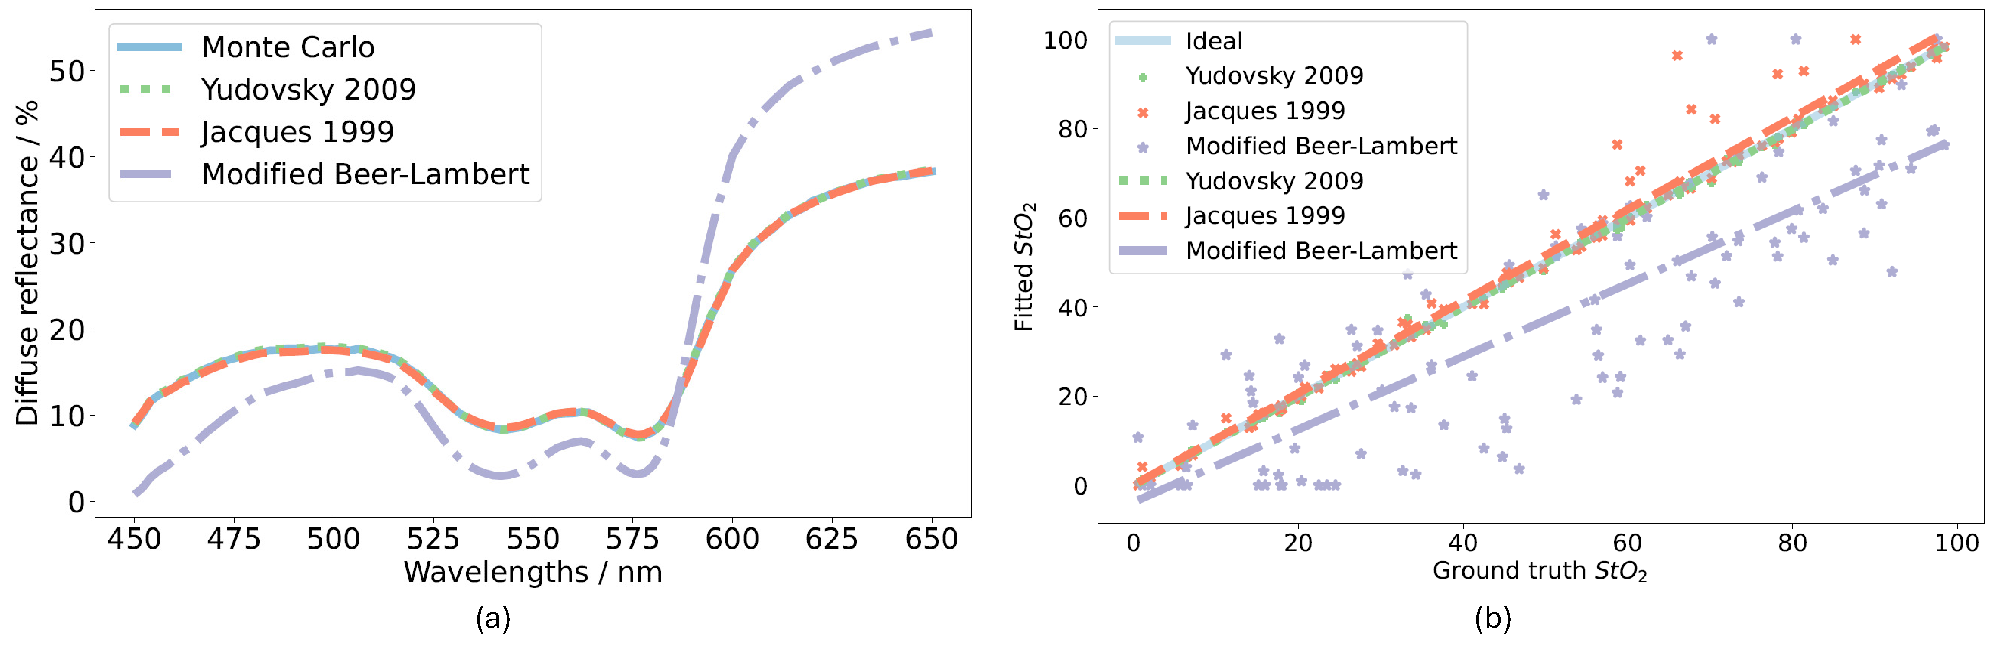
\includegraphics[width=\textwidth]{Figure_3.pdf}
    % \begin{subfigure}{0.49\textwidth}
    %     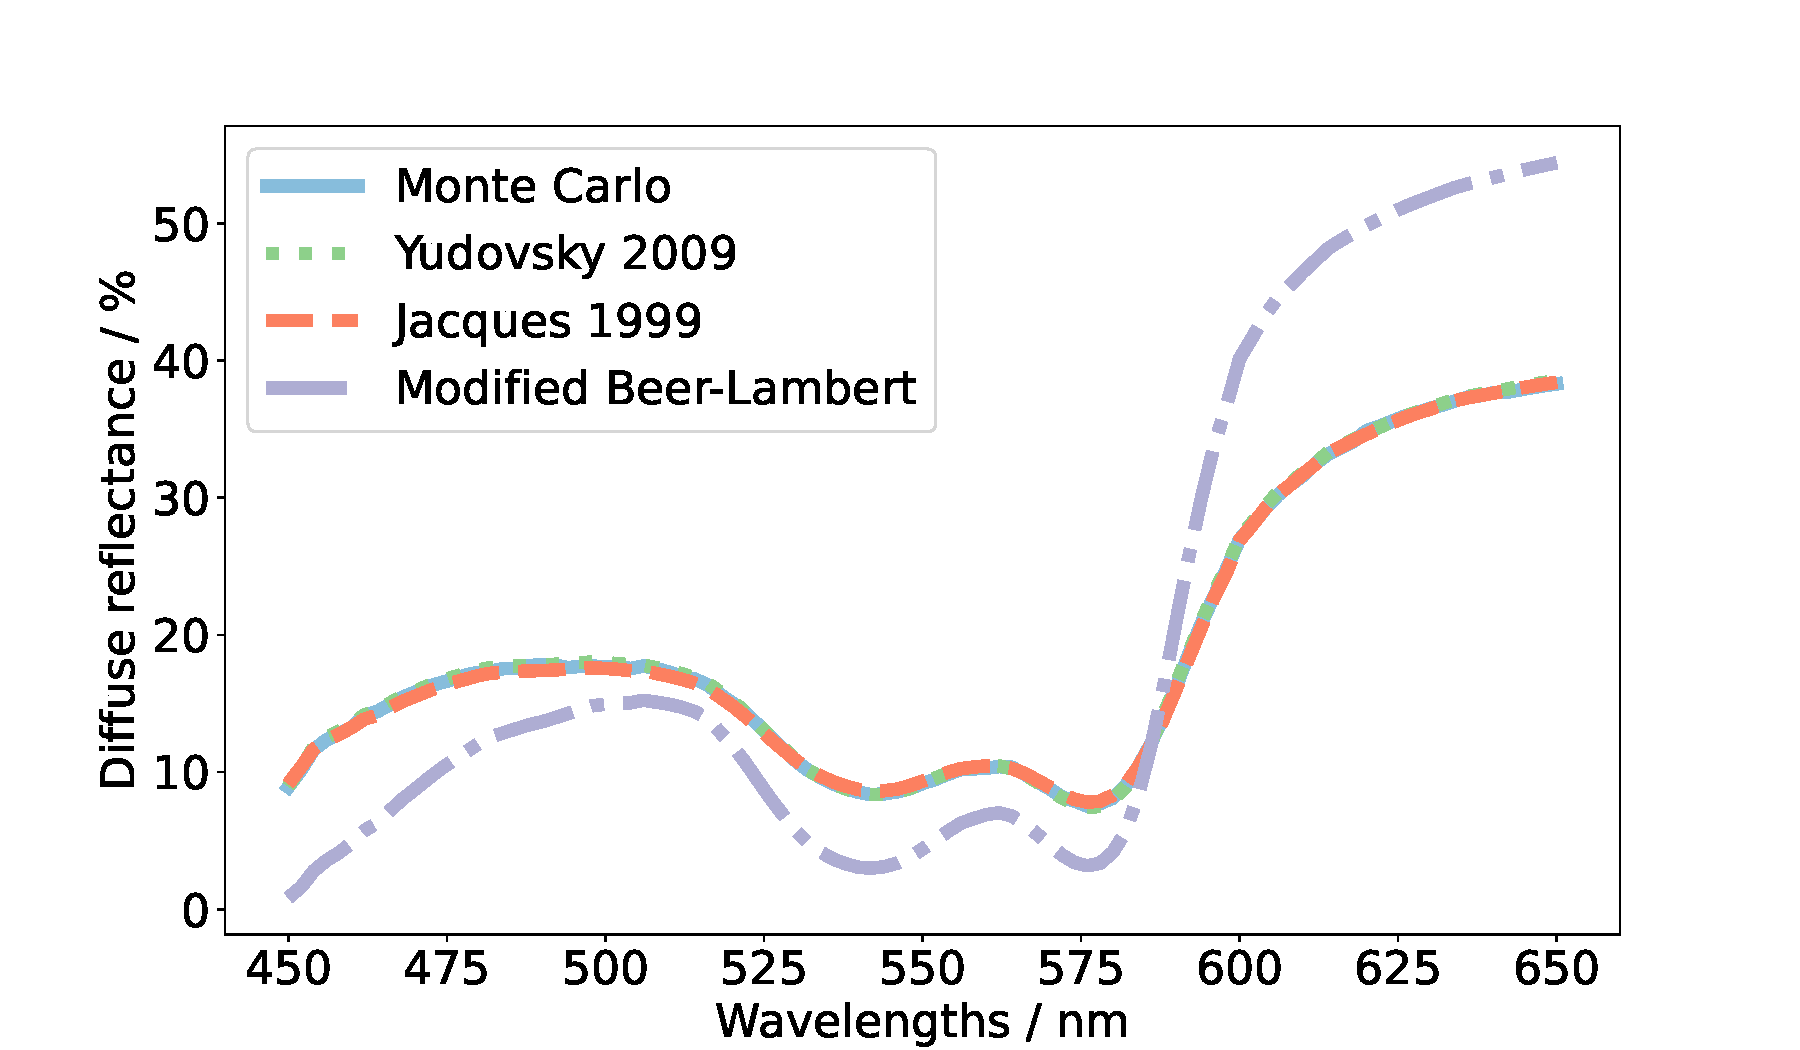
\includegraphics[width=\textwidth]{Figure_3a.pdf}
    %     \caption{}
    %     \label{fig:egspectrasingle}
    % \end{subfigure}
    % \begin{subfigure}{0.49\textwidth}
    %     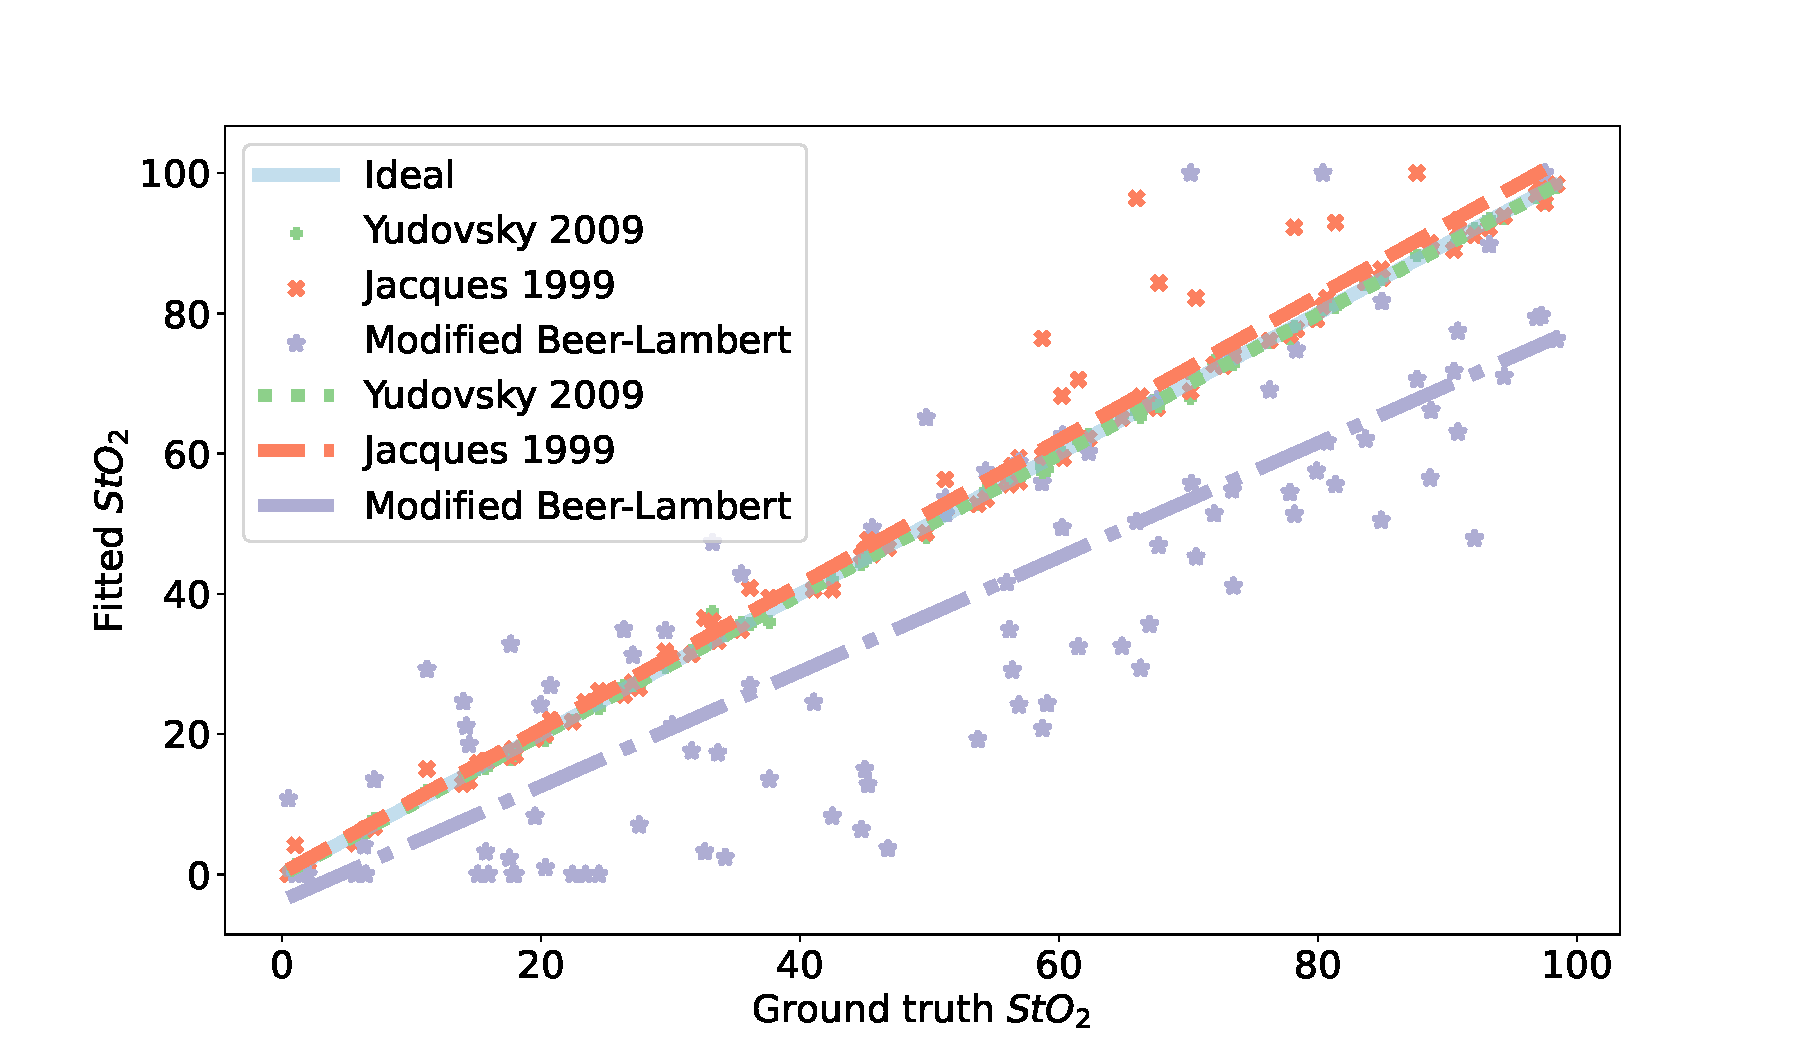
\includegraphics[width=\textwidth]{Figure_3b.pdf}
    %     \caption{}
    %     \label{fig:egtrendsingle}
    % \end{subfigure}
    \caption{Figure depicting evaluation of forward models (a) and inverse problem solutions (b). 
    Figure a depicts an example of the predicted spectra from each forward analytical model: Yudovsky 2009 (\textcolor{MyGreen}{green dotted}), Jacques 1999 (\textcolor{MyOrange}{orange dashed}), and Modified Beer-Lambert (\textcolor{MyPurple}{purple dot-dashed}), using ground truth variables for a refractive index of 1.44 compared to that predicted by MC (\textcolor{MyBlue}{blue solid}).
    Figure b shows an example of difference in quality of parameter recovery by fitting each inverse analytical model to MC simulations in the wavelength range of 450-600nm: Yudovsky 2009 (\textcolor{MyGreen}{green $+$}), Jacques 1999 (\textcolor{MyOrange}{orange $\times$}), and Modified Beer-Lambert (\textcolor{MyPurple}{purple $*$}), and their associated trend lines for a refractive index of 1.44 for $StO_2$.}
    \label{fig:FwDandInverse}
\end{figure}

\begin{table}[htpb]
    \centering
    \caption{The  Pearson $r$ (bold if $p<0.05$) of the linear regression line between the fitted tissue parameters and their ground truth displayed with their median (inter-quartile range) absolute percentage errors ($APE$). This is shown for each variable and for a refractive index of 1.44 when extracted by fitting Yudovsky 2009 (Y), Jacques 1999 (J), or Modified Beer-Lambert (BL) to the Monte-Carlo dataset in the wavelength range 450-600nm. All presented to 3s.f.}
    \begin{tabular}{|cc|cc|}
        \hline
        parameter & model & $r$ & median (inter-quartile range) \\
        & &  & $APE$ (\%)\\
        \hline
        \multirow{3}{*}{$StO_2$} & Y & \textbf{1.00} & 0.913 (1.92) \\
        % \cline{2-5}
        & J & \textbf{0.986} & 2.21 (4.97) \\
        % \cline{2-5}
        & BL & \textbf{0.838} & 43.0 (49.8) \\
        \hline
        \multirow{3}{*}{$f_{blood}$} & Y & \textbf{0.982} & 5.68 (6.08) \\
        % \cline{2-5}
        & J & \textbf{0.928} & 7.26 (16.2) \\
        % \cline{2-5}
        & BL & \textbf{0.582} & 49.6 (32.2) \\
        \hline
        \multirow{3}{*}{$a$} & Y & \textbf{0.992} & 3.90 (4.73) \\
        % \cline{2-5}
        & J & \textbf{0.959} & 4.54 (15.3) \\
        % \cline{2-5}
        & BL & \textbf{-0.706} & 40.0 (114) \\
        \hline
        \multirow{3}{*}{$b$} & Y & \textbf{1.00} & 1.50 (2.92) \\
        % \cline{2-5}
        & J & \textbf{0.963} & 2.86 (9.11) \\
        % \cline{2-5}
        & BL & \textbf{-0.446} & 95.4 (5.68) \\
        \hline
    \end{tabular}
    \label{tb:singleparamtrends}
\end{table}

Finally, the inverse problems with our fixed hyperparameters are fitted as in \ref{sec:methodevaluate} to this same MC dataset to recover the $StO_2$, $f_{blood}$, $a$, and $b$ tissue parameters. A linear regression is fitted between these retrieved values and the ground truth counterparts. The Pearson $r$ values of this, and the median (inter-quartile range) absolute percentage errors between the fitted and ground truth tissue parameters are shown in Table \ref{tb:singleparamtrends} for a refractive index of 1.44 with further parameters and refractive indices shown in Appendix Table \ref{tb:singleparamtrendsfull}. An example of the fitted parameters compared to the ground truth parameters is shown for $StO_2$ at a refractive index of 1.44 in Figure \ref{fig:FwDandInverse}b. 



% \begin{figure}
%     \centering
%     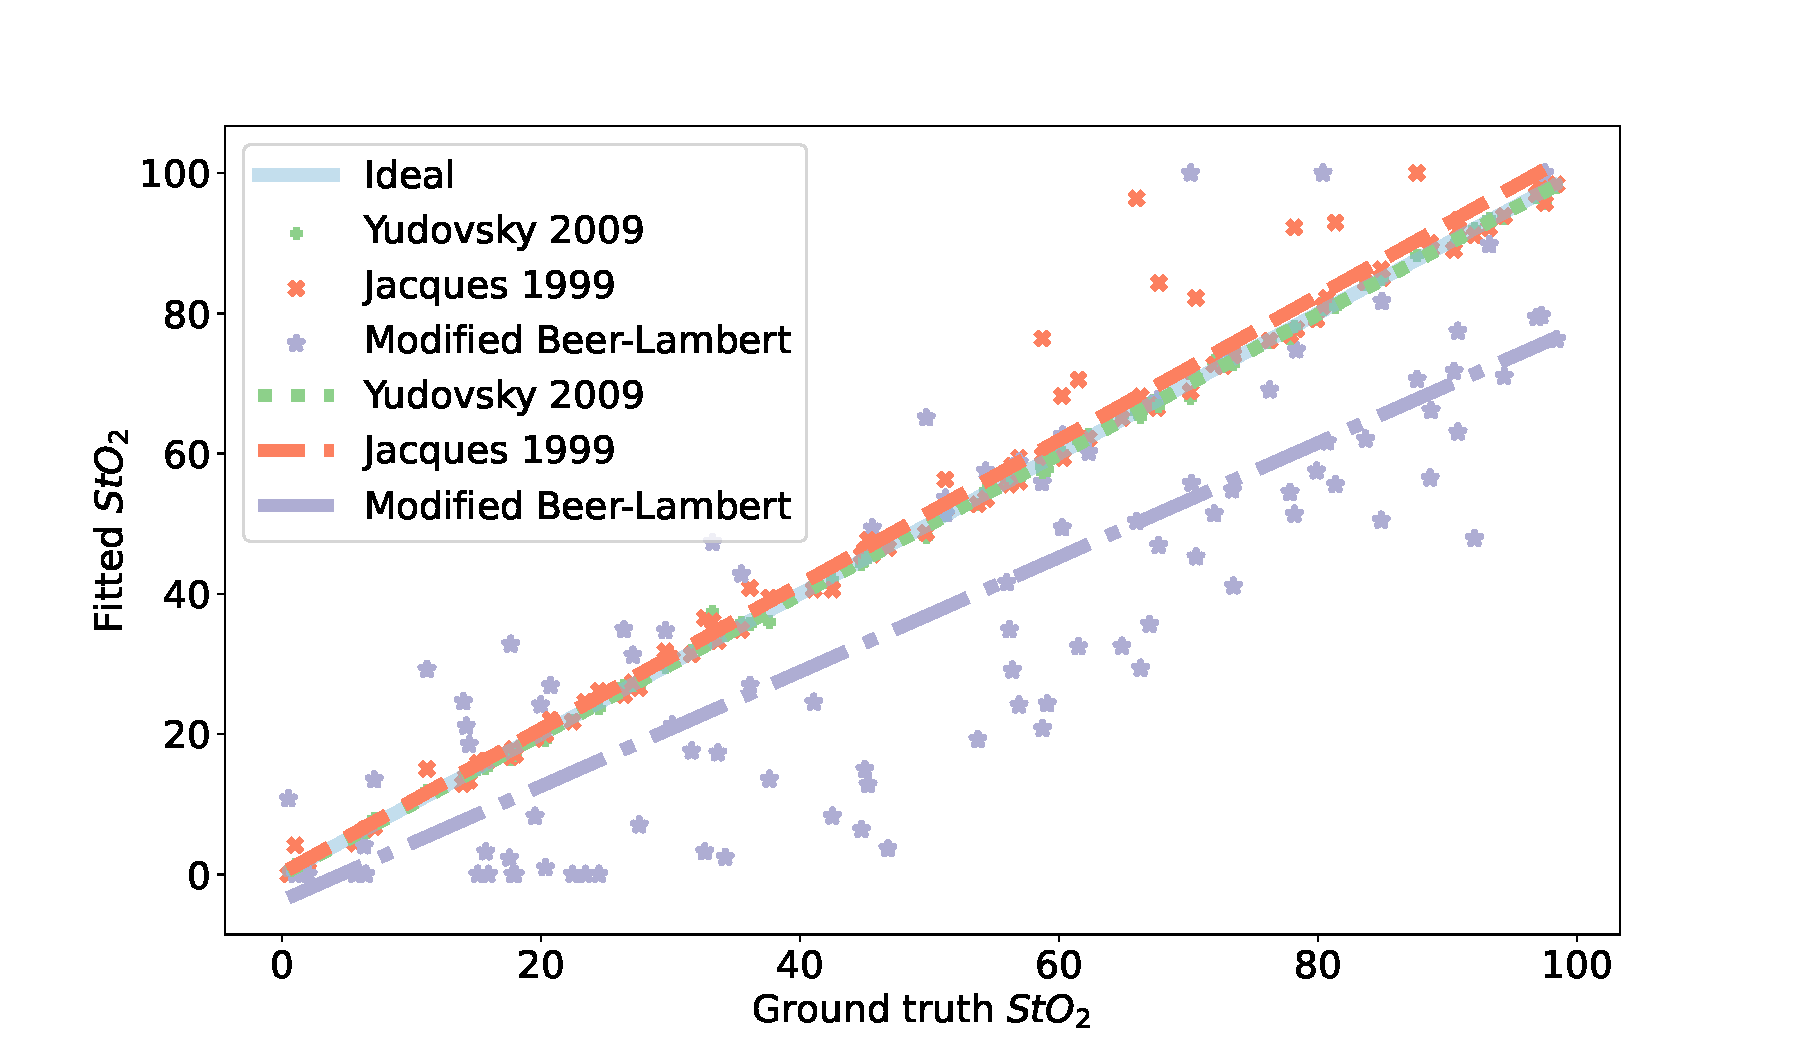
\includegraphics[width=0.7\textwidth]{StO2_1.44}
%     \caption{Example of difference in quality of parameter recovery by fitting each inverse analytical model to MC simulations: Yudovsky 2009 (green $+$), Jacques 1999 (red $\times$), and Modified Beer-Lambert (orange $*$), and their associated trendlines for a refractive index of 1.44 for $StO_2$.}
%  \label{fig:egtrendsingle}
% \end{figure}

%\FloatBarrier
\subsection{Gelatin-based tissue phantoms}\label{sec:resultsPhantoms}
Each dye absorbance is measured in both an aqueous and gelatin based solution with effective extinction coefficients calculated in each case. Whilst the aqueous measurements closely match the expected $\epsilon_{eff}(\lambda)$ from literature\cite{PhotochemCAD}, the gelatin measurements show a shifting of peaks, as seen in Figure~\ref{fig:Phantombackgrounds}a. This is likely due to interaction of the dyes with gelatin altering their interactions with solvent as has been noted with other dyes \cite{Cook2011}.
Since these peak shifts are seen in all subsequent data, these gelatin-based $\epsilon_{eff}(\lambda)$ are used in the model analysis. A pure gelatin solution absorption is measured at the concentration used in each phantom. This is used as a background $\mu_a(\lambda)$, as seen in Figure~\ref{fig:muaback}, to account for any absorption not due to dyes.
We further assume that intralipid is a purely scattering medium. This is considered a reasonable assumption since the IAD returned $\mu_a$ for the purely intralipid phantoms are similar to the pure gelatin background $\mu_a$ seen in Figure~\ref{fig:muaback}.

\begin{figure}[htb!]
    \centering
    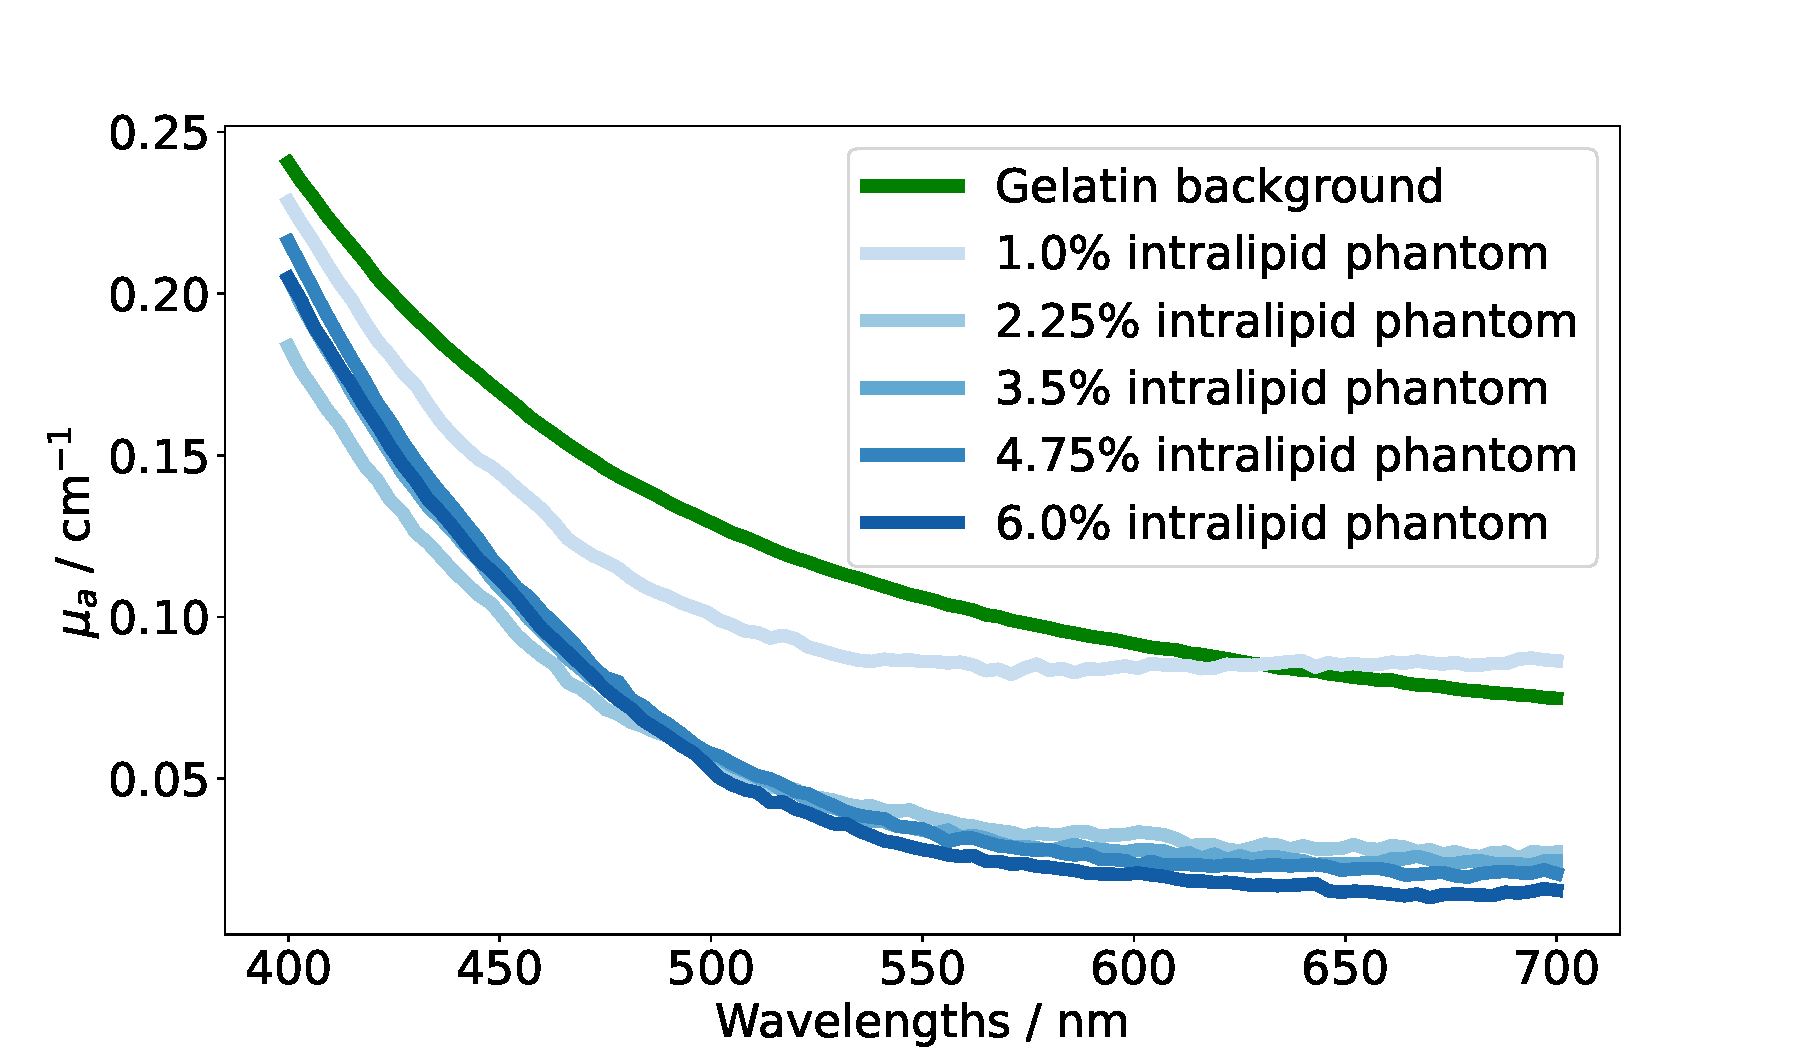
\includegraphics[width=0.6\textwidth]{Figure_A2.pdf}
    \caption{Background $\mu_a$ using absorption of pure gelatin solution compared to the IAD returned $\mu_a$ of the phantoms containing intralipid but no dyes.}
 \label{fig:muaback}
\end{figure}
% \FloatBarrier

% \section{}\label{ap:atrend}
\begin{figure}[h!]
    \centering
    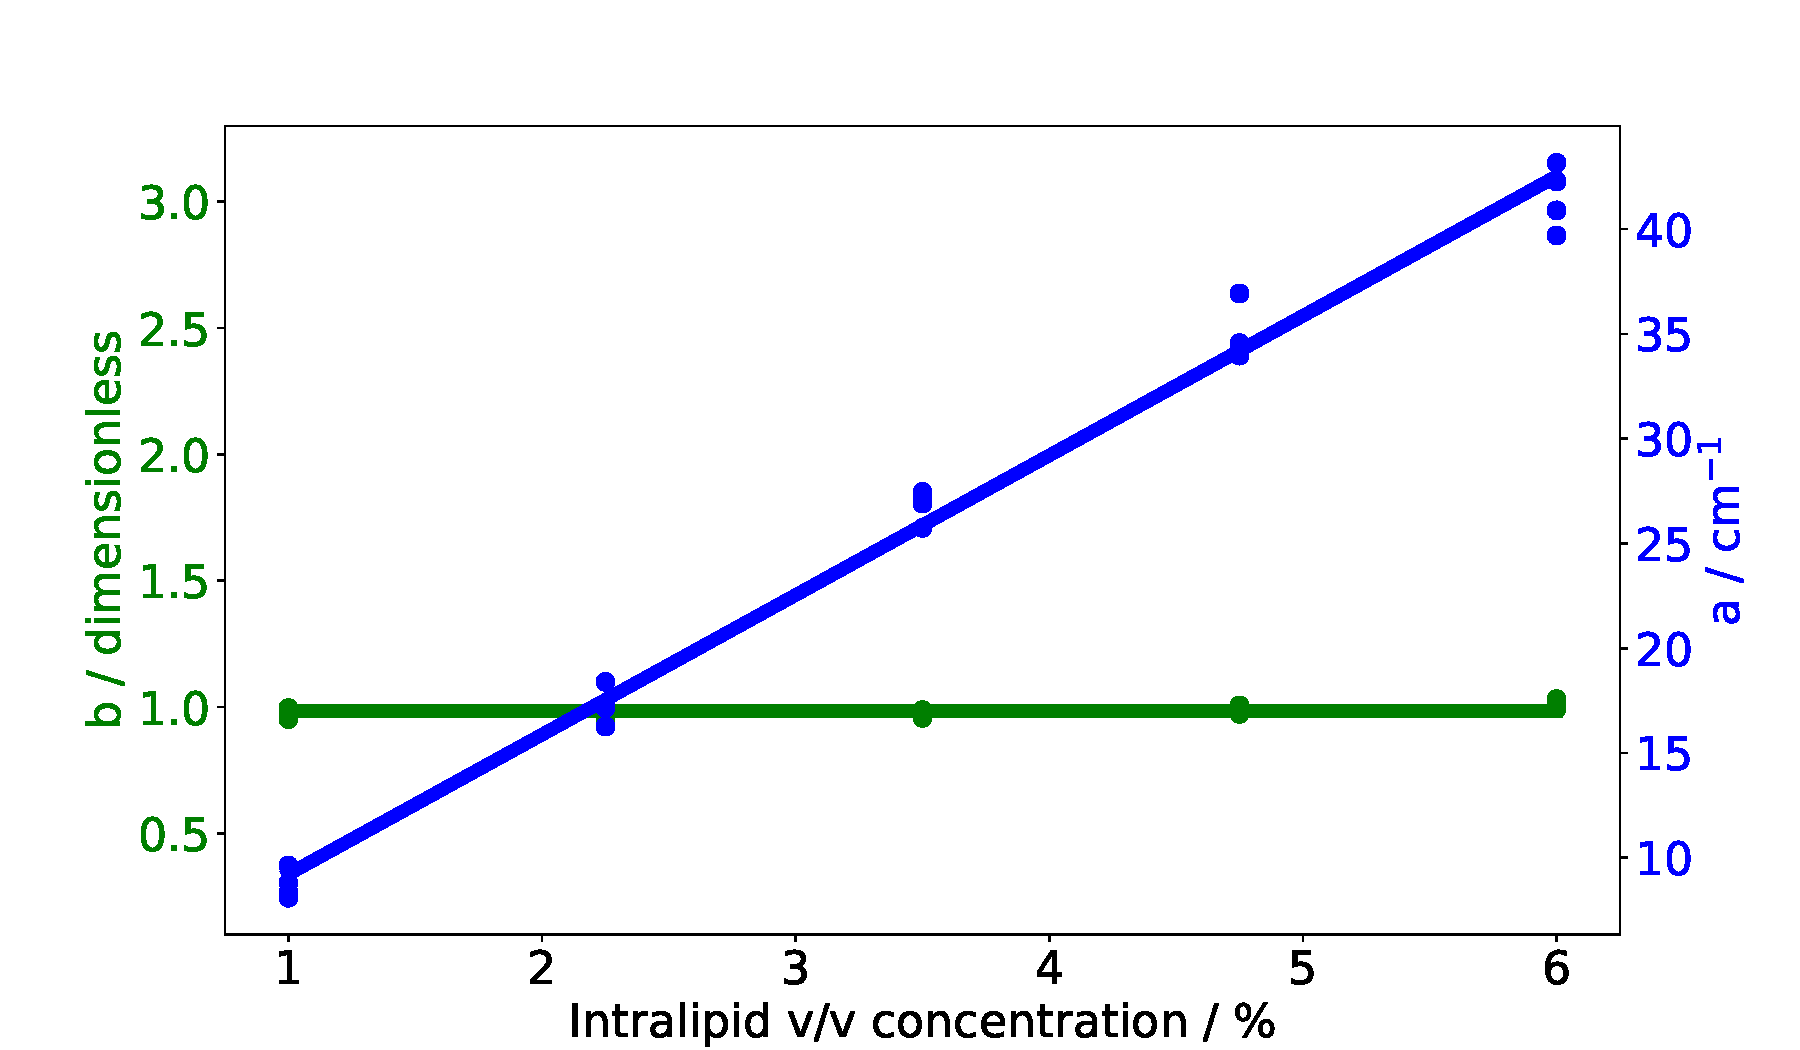
\includegraphics[width=0.6\textwidth]{Figure_A3.pdf}
    \caption{Trend in $a$ with intralipid concentration alongside linear regression. The trend in $b$ with intralipid concentration is also plotted alongside the median $b$ value.}
 \label{fig:atrend}
\end{figure}
% \begin{figure}
%     \centering
%     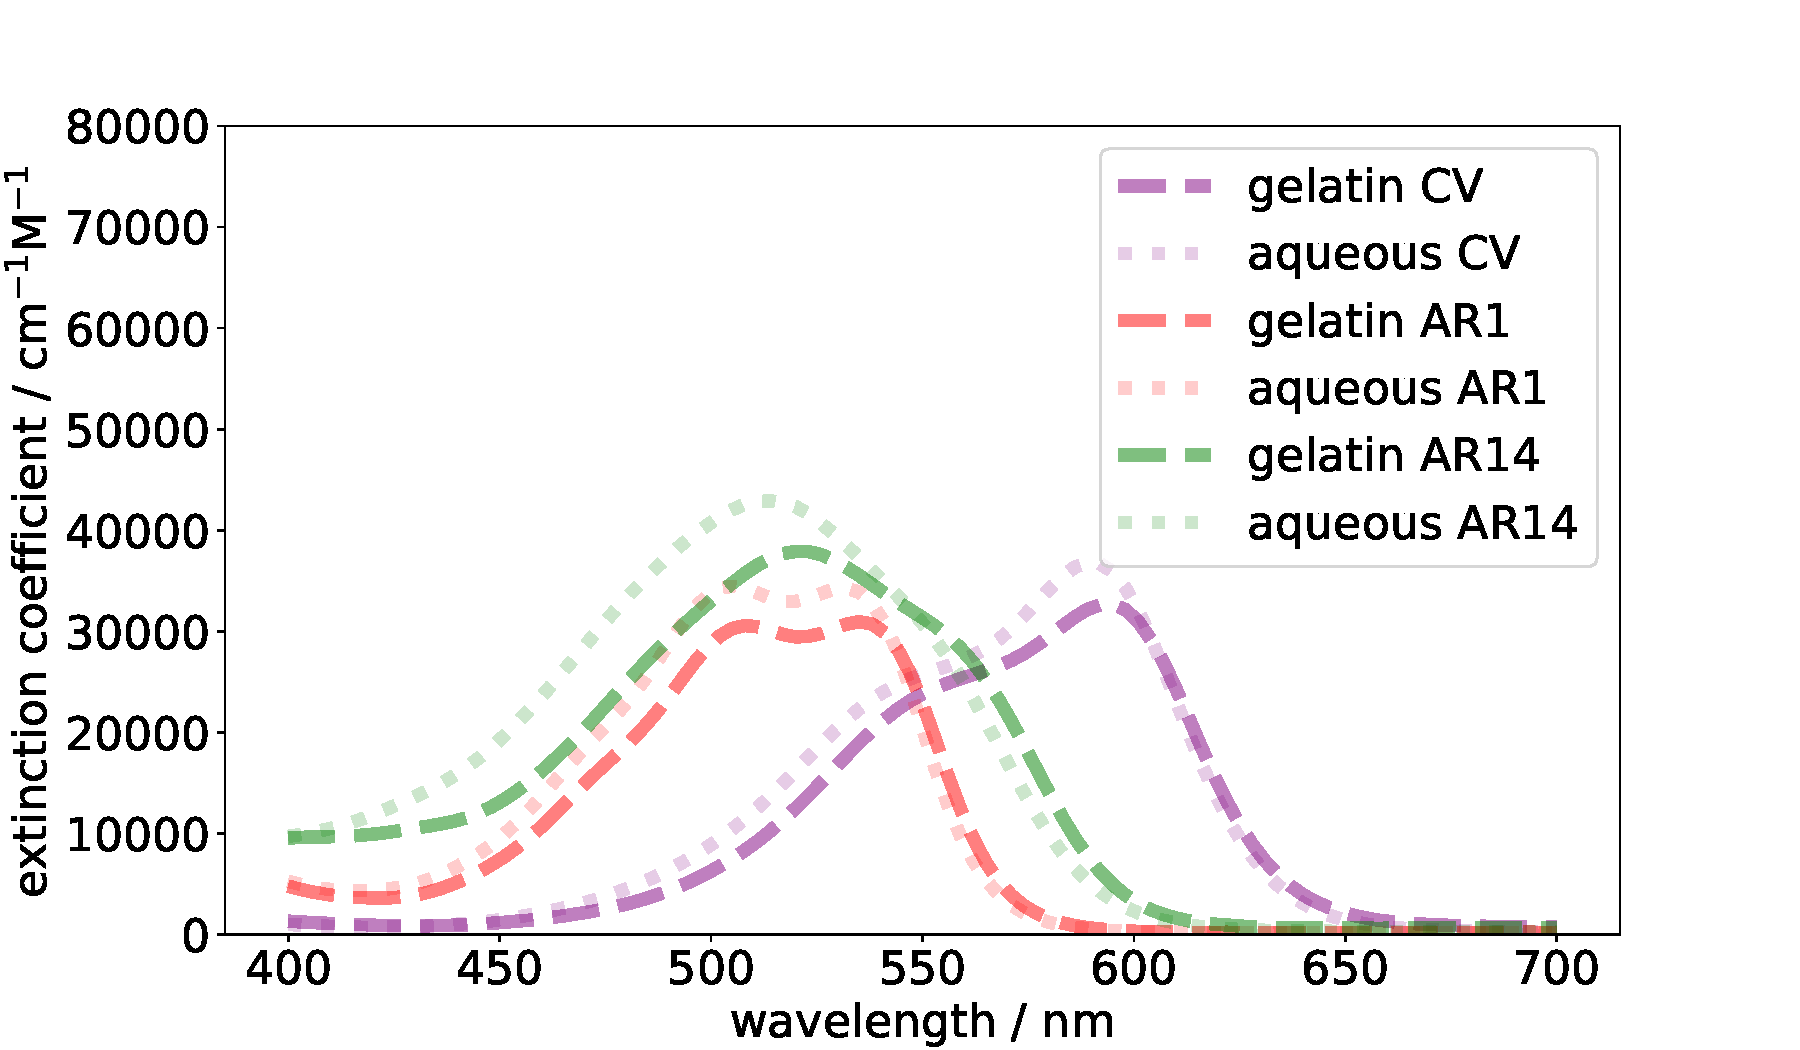
\includegraphics[width=0.65\textwidth]{mean_effective_eps_vs_scaled_lit.pdf}
%     \caption{$\epsilon_{eff}$ calculated for each dye [acid red 1 (AR1), acid red 14 (AR14), crystal violet (CV)] measured in gelatin (dashed) or PBS (dotted) compared to those expected from literature (solid) demonstrating the shift in peaks.}
%  \label{fig:epseff}
% \end{figure}
% \begin{figure}
%     \centering
%     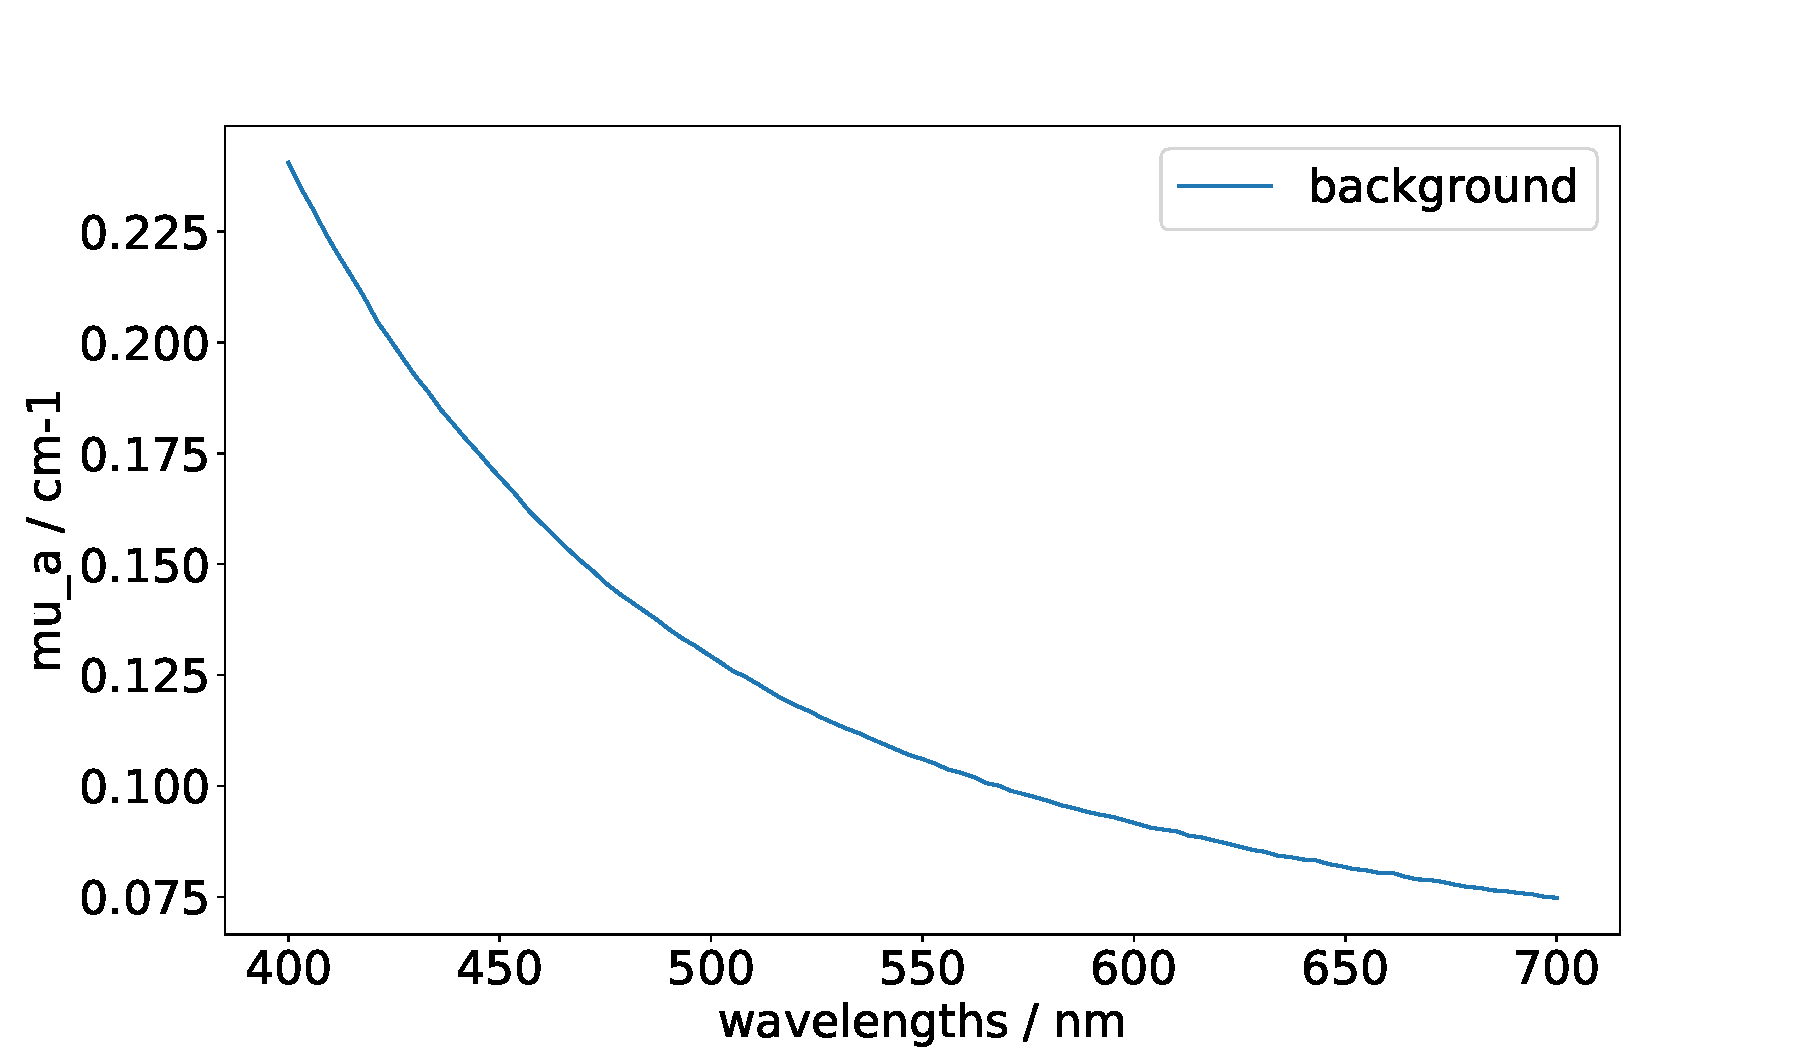
\includegraphics[width=0.8\textwidth]{mua_background.pdf}
%     \caption{Background $\mu_a$ using absorption of pure gelatin solution.}
%  \label{fig:muaback}
% \end{figure}

IAD\cite{Prahl2017} is used to analyse phantoms of 5mm depth with or without dyes in all intralipid concentrations. The $a$ and $b$ Mie coefficients fitted to the scattering in these cases are plotted against intralipid concentration. It was found that $b$ had no significant trend with intralipid concentration and so a median value of 0.98 was used in this work.
However, a clear trend was identified for $a$ as can be seen in Figure \ref{fig:atrend}. 
This trend is described in Equation \eqref{eq:atrend}, where $I$ is the intralipid concentration and $I_0$ is the reference concentration of 1\%v/v: 
\begin{equation}
    a = 6.66cm^{-1}\frac{I}{I_0} + 2.55cm^{-1}
    \label{eq:atrend}
\end{equation}
A Pearson correlation coefficient ($r$) of 0.99 and p of 0.00 was observed, therefore this is used throughout this work to model scattering based on Intralipid concentration.
% \begin{figure}
%     \centering
%     \includegraphics[width=0.8\textwidth]{a_trend.pdf}
%     \caption{Trend in $a$ with change in intralipid concentration.}
%  \label{fig:atrend}
% \end{figure}

The calculated $\mu_a(\lambda)$ using $\epsilon_{eff}(\lambda)$ displayed in Figure \ref{fig:Phantombackgrounds}a is compared to the IAD outputs of phantoms including dyes with each intralipid concentration.
An example of this is seen in Figure \ref{fig:Phantombackgrounds}b. This shows the overall spectrum is accurate, however the peak for CV (approx 600nm) appears shifted in wavelength, likely due to interactions with intralipid which cannot be captured in absorbance measurements. 
% \begin{figure}
%     \centering
%     \includegraphics[width=0.65\textwidth]{14.pdf}
%     \caption{Calculated (black solid) $\mu_a$ for one 3-dye configuration compared to the IAD output $\mu_a$ (coloured dashed) from measurements of phantoms in this configuration with a range of intralipid concentrations.}
%  \label{fig:IADmua}
% \end{figure}

\begin{figure}[htbp]
    \centering
    \includegraphics[width=\textwidth]{Figure_4.pdf}
    % \begin{subfigure}{0.49\textwidth}
    %     \includegraphics[width=\textwidth]{Figure_4a.pdf}
    %     \caption{}
    %     \label{fig:epseff}
    % \end{subfigure}
    % \begin{subfigure}{0.49\textwidth}
    %     \includegraphics[width=\textwidth]{Figure_4b.pdf}
    %     \caption{}
    %     \label{fig:IADmua}
    % \end{subfigure}
    \caption{Figure a shows $\epsilon_{eff}(\lambda)$ calculated for each dye [acid red 1 (AR1), acid red 14 (AR14), crystal violet (CV)] measured in gelatin (dashed) or PBS (dotted) demonstrating the shift in peaks. Figure b shows a calculated (black solid) $\mu_a(\lambda)$ for one 3-dye configuration compared to the IAD output $\mu_a(\lambda)$ (coloured dashed) from measurements of phantoms in this configuration with a range of intralipid concentrations.}
    \label{fig:Phantombackgrounds}
\end{figure}

Using a refractive index of 1.35\cite{Pogue2006} diffuse reflectance spectra are generated from each model using $\mu_a(\lambda)$ and $\mu_s'(\lambda)$ from Equations~\eqref{eq:phantommua} and \eqref{eq:Mie} using the trend in Equation \eqref{eq:atrend} and the median $b$ value for each 2-dye configuration and intralipid concentration. The forward Yudovsky, Jacques, and Modified Beer-Lambert models in Section \ref{sec:resultsMC} are compared to diffuse reflectance measurements for each phantom.
An example of this can be seen in Figure \ref{fig:phantomforwards}a for quantitative spectra or Figure \ref{fig:phantomforwards}c for mean normalised relative data.
The data is normalised using the mean of the wavelength range 450-575nm as beyond this region the models appear to fit poorly as seen in Figure \ref{fig:phantomforwards}b. 
The mean $NRMSE$ ($\pm$ standard deviation) between each spectrum and the measured spectrum, in the region 450-575nm, for this dataset can be seen in Table \ref{tb:NRMSEphantom}. 
The Pearson correlation coefficient $r$ between the forwards spectra compared to the measured spectra for each model is shown in Table \ref{tb:NRMSEphantom} and further parameters in Appendix Table \ref{tb:phantomparamsfull}. Whilst the overall magnitude of these is higher, the trend in quality of fit is similar as to the MC simulations. 

The inverse problems are solved by non-linear least squares  approaches using measured spectrum as reference observations. The recovered parameters are correlated to the ground truth parameters. The associated errors and correlation coefficients can be seen in Table \ref{tb:NRMSEphantom} (and further in Appendix Table \ref{tb:phantomparamsfull}) and an example of the fitted parameters compared to ground truth parameters is shown for $AR1$ in Figure~\ref{fig:phantomforwards}d for fits to quantitative spectra or Figure~\ref{fig:phantomforwards}e for fits to 
relative spectra.
% ratio-based parameters.

\begin{figure}[htbp]
    \centering
    \includegraphics[width=\textwidth]{Figure_5.pdf}
    % \begin{subfigure}{0.33\textwidth}
    %     \includegraphics[width=\textwidth]{Figure_5a.pdf}
    %     \caption{}
    %     \label{fig:phantomforwardsquant}
    % \end{subfigure}
    % \begin{subfigure}{0.33\textwidth}
    %     \includegraphics[width=\textwidth]{Figure_5b.pdf}
    %     \caption{}
    %     \label{fig:phantomresidual}
    % \end{subfigure}
    % \begin{subfigure}{0.33\textwidth}
    %     \includegraphics[width=\textwidth]{Figure_5c.pdf}
    %     \caption{}
    %     \label{fig:phantomforwardsnorm}
    % \end{subfigure}
    % \hfill
    % \begin{subfigure}{0.49\textwidth}
    %     \includegraphics[width=\textwidth]{Figure_5d.pdf}
    %     \caption{}
    %     \label{fig:phantomAR1quant}
    % \end{subfigure}
    % \begin{subfigure}{0.49\textwidth}
    %     \includegraphics[width=\textwidth]{Figure_5e.pdf}
    %     \caption{}
    %     \label{fig:phantomAR1norm}
    % \end{subfigure}
    \caption{Example of measured (\textcolor{MyBlue}{blue}) spectrum for one 2-dye configuration at an intralipid concentration of 3.5\% compared to the respective spectra generated from the Yudovsky 2009 (\textcolor{MyGreen}{green dotted}), Jacques 1999 (\textcolor{MyOrange}{orange dashed}), and Modified Beer-Lambert (\textcolor{MyPurple}{purple dot-dashed}) models using the ground truth parameters for quantitative (a) or relative (c) spectra (mean normalised in the range 450-575nm). The residuals between the modelled quantitative spectra and the measured spectra are shown in b. Examples of the parameter recovery from the measured phantom spectra for the AR1 proportion by Yudovsky 2009 (\textcolor{MyGreen}{green +}), Jacques 1999 (\textcolor{MyOrange}{orange $\times$)}, and Modified Beer-Lambert (\textcolor{MyPurple}{purple $*$}) models compared with the ground truth parameters (\textcolor{MyBlue}{blue solid}) for fits to quantitative (d) or relative (e) spectra in the wavelength range 450-575nm.}
 \label{fig:phantomforwards}
\end{figure}

\begin{table}[htbp]
    \centering
    \caption{mean ($\pm$ standard deviation) $NRMSE$ (3.d.p.) between the modelled spectrum using the ground truth parameters and the measured spectrum of a tissue phantom for each analytical model for either quantitative or relative spectra. Alongside this is the Pearson $r$ (bold if $p < 0.05$) for each model for all forwards spectra compared to the measured spectra. All metrics evaluated for the wavelength range 450-575nm}
    \begin{tabular}{|c|c|c|c|}
        \hline 
        Model & Quantitative (Q) or Relative (R) & $NRMSE$ & $r$ \\
        \hline
        \multirow{2}{*}{Yudovsky 2009} & Q & 0.059 ($\pm$ 0.031) & \textbf{0.998} \\
        & R & 0.012 ($\pm$ 0.009) & \textbf{0.999} \\
        \hline
        \multirow{2}{*}{Jacques 1999} & Q & 0.075 ($\pm$ 0.032) & \textbf{0.998} \\
        & R & 0.022 ($\pm$ 0.023) & \textbf{0.995} \\
        \hline
        \multirow{2}{*}{Modified Beer-Lambert} & Q & 0.464 ($\pm$ 0.294) & \textbf{0.808} \\
        & R & 0.215 ($\pm$ 0.139) & \textbf{0.930} \\
        \hline
    \end{tabular}
    % \begin{tabular}{|c|c|c|c|}
    %     \hline
    %     \multirow{2}{*}{Quantitative (Q) or Relative (R)} & \multicolumn{3}{c|}{Model} \\
    %     & Yudovsky 2009 & Jacques 1999 & Modified Beer-Lambert \\
    %     \hline
    %     Q & 0.120 ($\pm$ 0.036) & 0.135 ($\pm$ 0.036) & 0.292 ($\pm$ 0.081) \\
    %     R & 0.077 ($\pm$ 0.036) & 0.083 ($\pm$ 0.048) & 0.376 ($\pm$ 0.363) \\
    %     \hline
    % \end{tabular}
    \label{tb:NRMSEphantom}
\end{table}

% \begin{figure}
%     \centering
%     \begin{subfigure}{0.7\textwidth}
%         \includegraphics[width=\textwidth]{AR1.pdf}
%         \caption{}
%         \label{fig:phantomAR1quant}
%     \end{subfigure}
%     \begin{subfigure}{0.7\textwidth}
%         \includegraphics[width=\textwidth]{AR1_norm.pdf}
%         \caption{}
%         \label{fig:phantomAR1norm}
%     \end{subfigure}
%     \caption{Examples of the parameter recovery from measured tissue phantom spectra for the AR1 proportion. The Yudovsky 2009 (green +), Jacques 1999 (red $\times$), and Modified Beer-Lambert (orange $*$) models using the ground truth parameters (blue solid) for fits to quantitative (\ref{fig:phantomAR1quant}) or relative (\ref{fig:phantomAR1norm}) spectra.}
%  \label{fig:phantomAR1}
% \end{figure}

\begin{table}[htbp]
    \centering
    \caption{The  Pearson $r$ (bold if $p<0.05$) of the linear regression line between the fitted parameters and their ground
    truth displayed with their median (inter-quartile range) absolute percentage errors for each variable when extracted by fitting Yudovsky 2009 (Y), Jacques 1999 (J), or Modified Beer-Lambert (BL) for both quantitative and relative data. All metrics calculated for the wavelength range 450-575nm and presented to 3s.f.}
    \begin{tabular}{|ccc|cc|}
        \hline
        Parameter & Model & Quantitative (Q) & $r$ & median (inter-quartile range) \\
        & & or Relative (R) & & $APE$ (\%)\\
        \hline
        \multirow{6}{*}{$AR1$} & \multirow{2}{*}{Y} & Q & \textbf{0.997} & 1.59 (11.0) \\
        & & R & \textbf{0.998} & 4.42 (8.31) \\
        \cline{2-5}
        & \multirow{2}{*}{J} & Q & \textbf{0.989} & 7.02 (20.2) \\
        & & R & \textbf{0.934} & 10.4 (23.7) \\
        \cline{2-5}
        & \multirow{2}{*}{BL} & Q & \textbf{0.756} & 83.5 (57.0) \\
        & & R & \textbf{0.939} & 50.0 (31.4)\\
        \hline
        \multirow{6}{*}{$AR14$} & \multirow{2}{*}{Y} & Q & \textbf{1.00} & 1.36 (8.69) \\
        & & R & \textbf{0.998} & 2.48 (5.76) \\
        \cline{2-5}
        & \multirow{2}{*}{J} & Q & \textbf{0.989} & 7.02 (16.3) \\
        & & R & \textbf{0.934} & 6.34 (10.0)\\
        \cline{2-5}
        & \multirow{2}{*}{BL} & Q & \textbf{0.756} & 80.4 (72.1) \\
        & & R & \textbf{0.939} & 37.5 (66.7) \\
        \hline
        \multirow{6}{*}{$I$} & \multirow{2}{*}{Y} & Q & \textbf{0.648} & 125 (276) \\
        & & R & 0.310 & 93.9 (30.0) \\
        \cline{2-5}
        & \multirow{2}{*}{J} & Q & \textbf{0.540} & 122 (288) \\
        & & R & \textbf{-0.451} & 100 (55.7) \\
        \cline{2-5}
        & \multirow{2}{*}{BL} & Q & \textbf{-0.705} & 100 (172) \\
        & & R & -0.157 & 100 (0.00) \\
        \hline
        \multirow{6}{*}{$c_{tot}$} & \multirow{2}{*}{Y} & Q &  \textbf{0.500} & 102 (226) \\
        & & R & 0.303 & 66.1 (46.8) \\
        \cline{2-5}
        & \multirow{2}{*}{J} & Q & \textbf{0.684} & 100 (260) \\
        & & R & -0.0959 & 89.7 (267)\\
        \cline{2-5}
        & \multirow{2}{*}{BL} & Q & \textbf{0.721} & 35.2 (21.6) \\
        & & R & \textbf{0.689} & 44.6 (23.6)\\
        \hline
    \end{tabular}
    \label{tb:phantomparams}
\end{table}

Finally, some 3-dye configurations are investigated with the addition of CV. Some examples of both quantitative and relative spectral reconstruction using the ground truth parameters in the forward Yudovsky model for a single 3-dye configuration at a range of intralipid concentrations can be seen in Figure \ref{ap:3phantomforwards}. 

\begin{figure}[htb!]
    \centering
    \includegraphics[width=\textwidth]{Figure_A4.pdf}
    % \begin{subfigure}{0.8\textwidth}
    %     \includegraphics[width=\textwidth]{Figure_A4a.pdf}
    %     \caption{}
    %     \label{fig:3phantomforwardsquant}
    % \end{subfigure}
    % \begin{subfigure}{0.8\textwidth}
    %     \includegraphics[width=\textwidth]{Figure_A4b.pdf}
    %     \caption{}
    %     \label{fig:3phantomforwardsnorm}
    % \end{subfigure}
    \caption{Examples of Measured (blue) spectrum for one 3-dye configuration at a variety of intralipid concentrations compared to the respective spectra generated from the Yudovsky 2009 (green dotted) model using the ground truth parameters to generate quantitative (a) or relative (b) spectra.}
 \label{ap:3phantomforwards}
\end{figure}

Despite considering the shift in CV peak due to gelatin, there appears to be a further shift, likely due to interactions with intralipid. This can be seen as an offset between the measured and reconstructed spectra in Figure \ref{ap:3phantomforwards} and appears to change with intralipid concentration. Due to the limited ground truth parameter range for these 3-dye configurations, only median percentage errors are presented for the inverse problem solution performance in Table \ref{tb:3phantomparams} alongside their inter-quartile range. These show a dramatic loss in accuracy of $AR1$ and $AR14$ recovery, despite good $CV$ recovery, likely due to the imperfect $CV$ absorbance modelling distorting the spectrum. 

\begin{table}[htb!]
    \centering
    \caption{The median (inter-quartile range) absolute percentage errors for each variable when extracted by fitting Yudovsky 2009 (Y), Jacques 1999 (J), or Modified Beer-Lambert (BL) to measured 3-dye tissue phantom spectra for both quantitative and relative data. All presented to 3s.f.}
    \begin{tabular}{|ccc|c|}
        \hline
        parameter & model & Quantitative (Q) & median (inter-quartile range) \\
        & & or Relative (R) & absolute percentage error (\%)\\
        \hline
        \multirow{6}{*}{$AR1$} & \multirow{2}{*}{Y} & Q & 22.7 (25.8) \\
        & & R & 14.9 (9.14) \\
        \cline{2-4}
        & \multirow{2}{*}{J} & Q & 30.6 (29.8) \\
        & & R & 49.1 (84.6) \\
        \cline{2-4}
        & \multirow{2}{*}{BL} & Q & 86.7 (58.3) \\
        & & R & 77.1 (63.5) \\
        \hline
        \multirow{6}{*}{$AR14$} & \multirow{2}{*}{Y} & Q & 25.3 (23.0) \\
        & & R & 40.4 (23.7) \\
        \cline{2-4}
        & \multirow{2}{*}{J} & Q & 28.0 (28.8) \\
        & & R & 97.3 (219) \\
        \cline{2-4}
        & \multirow{2}{*}{BL} & Q & 129 (74.7) \\
        & & R & 122 (113) \\
        \hline
        \multirow{6}{*}{$CV$} & \multirow{2}{*}{Y} & Q & 13.3 (20.7) \\
        & & R & 19.2 (16.1) \\
        \cline{2-4}
        & \multirow{2}{*}{J} & Q & 9.25 (17.0) \\
        & & R & 21.0 (79.4) \\
        \cline{2-4}
        & \multirow{2}{*}{BL} & Q & 19.0 (13.2) \\
        & & R & 17.4 (14.3) \\
        \hline
        \multirow{6}{*}{$I$} & \multirow{2}{*}{Y} & Q & 145 (285) \\
        & & R & 88.4 (17.9) \\
        \cline{2-4}
        & \multirow{2}{*}{J} & Q & 131 (231) \\
        & & R & 100 (11.2) \\
        \cline{2-4}
        & \multirow{2}{*}{BL} & Q & 100 (67.1) \\
        & & R & 100 (2.53 $\times 10^{-10}$) \\
        \hline
        \multirow{6}{*}{$c_{tot}$} & \multirow{2}{*}{Y} & Q & 100 (285) \\
        & & R & 63.2 (24.1) \\
        \cline{2-4}
        & \multirow{2}{*}{J} & Q & 100 (206) \\
        & & R & 81.0 (3510) \\
        \cline{2-4}
        & \multirow{2}{*}{BL} & Q & 36.3 (36.9) \\
        & & R & 45.7 (66.9) \\
        \hline
    \end{tabular}
    \label{tb:3phantomparams}
\end{table}

\FloatBarrier
\section{Discussion and future work}\label{sec:discussion}
When compared to MC simulations, the semi-empirical Yudovsky model performs best in terms of fit and parameter extraction, followed closely by the Jacques model. The Modified Beer-Lambert model, however, performs much more poorly. It is also noted that the Jacques model fits MC simulations significantly better after refitting the hyperparameters, however the Yudovsky model performs well using literature values provided that the simplified erratum model is used. 

When modelling tissue phantom spectra, it is important to have some prior knowledge of the phantoms. This allows accurate $\mu_a(\lambda)$ and $\mu_s'(\lambda)$ calculation, for example utilising the shift in dye peaks from their literature data, background gelatin absorbance, and the trend in Mie scattering parameters with intralipid concentration. Some variation is seen in IAD which may be due to inaccuracies in sample depth measurement or variations in spectral measurements. This suggests that it gives an indication of the optical properties of a sample, however it may not be precise. 

When modelling the measured tissue phantom diffuse reflectance spectra using the forward models, Yudovsky performs best followed closely by Jacques, with Modified Beer-Lambert performing significantly worse. The $NRMSE$ calculated for relative data is an improvement on those calculated for quantitative data, suggesting that these models are reproducing the shape of the spectra well even when relatively constant offsets are present. When introducing a third dye ($CV$) the absorbance peak of this dye is noticeably wavelength shifted in experimental measurements compared to the theoretical spectra which then appears distorted. This shift appears to change with varying concentrations of intralipid suggesting some interaction there. 

When fitting the models to experimental data for parameter recovery, Yudovsky and Jacques produce excellent parameter recovery for $AR1$ and $AR14$ in both quantitative and relative regimes. For $c_{tot}$ and $I$ no models were able to recover the parameters well, whereas all parameters were recovered well by Yudovsky and Jacques when fitted to MC data. This is suggestive of some overlap in the effects of $c_{tot}$ and $I$ on the spectra. In the three-dye configuration $CV$ is recovered reasonably, despite the peak being outside of the region considered for fitting. The shift in the $CV$ peak, however, distorts the rest of the spectrum leading to very poor recovery of all other parameters. This demonstrates the importance of prior understanding of the chromophores for any model to recover parameters accurately. 

This work is associated with some limitations.
Firstly, whilst every effort was made to synthesise optical phantoms resembling biological tissue, measurements of true biological tissue could not be used for this work due to a lack of reliable ground truth parameters in tissue. %\revref{1}{6}
%, alongside challenges in integration to the surgical work flow since the surgical procedure cannot continue during the in-vivo data capture process. 
Similarly, haemoglobin chromophores could not be utilised in the phantoms due to their oxygen sensitivity which could not be controlled within the spectrophotometer measurement set-up. This led us to rely on stable synthetic dyes instead
%\revref{1}{1}\textcolor{red}{
, which do not perfectly replicate the spectra of oxy and deoxyhaemoglobin. The major dye peaks maxima are approximately 45nm lower than the distinctive haemoglobin peaks which may contribute to different wavelength regions performing differently with these phantoms compared to biological samples
%}
. 
%\revref{2}{1}\textcolor{red}{
The factors chosen to allow approximately equal impact from each dye were chosen to ease synthesis and should be optimised. Since these factors are incorporated in both synthesis and analysis, it is believed that these do not impact the conclusions of this study.
%}\revref{2}{5}\textcolor{red}{
The difference in extinction coefficient found when measuring each dye in gelatin compared to aqueous solution is not fully understood and requires further study.
%}\revref{1}{2}\textcolor{red}{
These phantoms are also spatially uniform meaning that, whilst these could be used to determine the performance of these models spatially using hyperspectral imaging systems, other methods would be required to assess spatial resolution of these systems \cite{EdmundOptics2023, Torkildsen2018}.
%}
%
Secondly, the shift in absorbance of the third chromophore made it difficult to model thereby limiting the investigation of the impact of additional chromophores.
%
Thirdly, whilst the IAD method produces results similar to our ground truth, there remain some differences between IAD output and the expected ground truth.
This could impact the quality of the intralipid scattering model used in this work.
%
Fourthly, these models assume a planar surface for measurement, however the surface may deviate from this. In these cases, Spatial Frequency Domain methods may be an alternative to obtain accurate $\mu_a$ and $\mu_s'$ values for tissues\cite{Gioux2019}. 
%Whilst Spatial Frequency Domain methods could be used to obtain ground truth $\mu_a$ and $\mu_s'$, analytical models are required to determine the $StO_2$ (or other parameters) from this\cite{Gioux2019} meaning that a true ground truth parameter from in vivo tissue measurement was not possible. 
Finally, the precise measurement of extinction coefficients of haemoglobin in biological tissue is not possible due to the scattering nature of these media.
However, it is shown in our work that the medium chosen for the dye can have an impact on the extinction coefficients and therefore the quality of the models. For this reason, the optical properties of tissue must be well defined to mimic the quality of results in this work.

Future work should include 
%investigation of these models for use with hyperspectral imaging cameras which may not have as densely sampled spectra as these have been shown to be likely methods of obtaining these diffuse reflectance spectra intra-operatively. \cite{Clancy2020}. 
%\revref{2}{5}\textcolor{red}{
%The impact of the medium on the dye extinction coefficients should be further investigated and understood.
investigating and understanding the impact of the medium on the dye extinction coefficients.
%}
There could also be greater investigation of including further chromophores whose absorbance behaviour is well modelled and optimisation of the fitting region. 
%Two-layer models should also be considered for tissue structures which exist in layered configurations, such as skin. 
%\revref{2}{6}\textcolor{red}{
Finally, similar analyses could be conducted in other wavelength ranges including the near infra-red range which can also be used for perfusion analysis with bespoke light sources \cite{Hummler2020}.
%}

In conclusion, the Yudovsky single layer model works well for modelling of tissue that can be approximated by a semi-infinite, homogeneous slab. Jacques is also able to well approximate this with a simpler model. All models require appropriate prior knowledge of the $mu_a$ and $mu_s'$ properties of the tissues to allow for a good quality of parameter recovery.

Since this investigation shows Yudovsky to be the most robust model, the layered model is similarly investigated in the following chapter. These models are also adapted for use with snapshot HSI data in Chapter \ref{chap:HSImodel}. 

% \section*{Acknowledgements}
% The authors would like to thank Jenasee Mynerich of King's College London who provided the CT imaging for the tissue phantom work presented.

% This study/project is funded by the NIHR [NIHR202114]. The views expressed are those of the author(s) and not necessarily those of the NIHR or the Department of Health and Social Care. 
% %
% This work was supported by core funding from the Wellcome/EPSRC [WT203148/Z/16/Z; NS/A000049/1].
% %
% TV is supported by a Medtronic / RAEng Research Chair [RCSRF1819\textbackslash7\textbackslash34].

% TV and JS are co-founders and shareholders of Hypervision Surgical Ltd, London, UK.

% For the purpose of open access, the authors have applied a CC BY public copyright licence to any Author Accepted Manuscript version arising from this submission.

% \bibliography{Paper2}

% % \appendix
\appendix
% \section{}\label{ap:MChyperparams}
\begin{table}[htb!]
    \centering
    \caption{Table displaying single layer model hyperparameters fitted to Monte Carlo datasets of each refractive index (black) with available literature values (blue).}
    \begin{tabular}{|cc|cc|c|cc|}
        \hline
        \multirow{2}{*}{Model} & \multirow{2}{*}{Parameter} & \multicolumn{5}{c|}{Refractive index} \\
         & & \multicolumn{2}{c|}{1.33} & 1.35 & \multicolumn{2}{c|}{1.44} \\
        \hline
        \multirow{6}{*}{Yudovsky 2009} & $M_1$ & \multicolumn{2}{c|}{-0.0253} & -0.0257 & -0.0254 & \textcolor{blue}{-0.0247} \\
        & $M_2$ & \multicolumn{2}{c|}{0.0166} & 0.0159 & 0.0135 & \textcolor{blue}{0.0137} \\
        & $M_3$ & \multicolumn{2}{c|}{2.873} & 2.873 & 2.873 & \textcolor{blue}{2.873} \\
        & $M_4$ & \multicolumn{2}{c|}{1.64} & 1.64 & 1.64 & \textcolor{blue}{1.64} \\
        & $M_5$ & \multicolumn{2}{c|}{0.0123} & 0.0124 & 0.0120 & \textcolor{blue}{0.0116} \\
        & $M_6$ & \multicolumn{2}{c|}{1.02} & 1.02 & 1.02 & \textcolor{blue}{1.02} \\
        \hline 
        \multirow{3}{*}{Jacques 1999} & $M_1$ & 7.0188 & \textcolor{blue}{6.3744} & 7.1185 & \multicolumn{2}{c|}{7.0438} \\
        & $M_2$ & 0.2464 & \textcolor{blue}{0.35688} & 0.2750 & \multicolumn{2}{c|}{0.6902} \\
        & $M_3$ & 4.2241 & \textcolor{blue}{3.4739} & 4.2571 & \multicolumn{2}{c|}{4.1449} \\
        \hline
        \multirow{3}{*}{Modified Beer-Lambert} & $M_1$ & \multicolumn{2}{c|}{0.283} & 0.308 & \multicolumn{2}{c|}{0.256} \\
        & $M_2$ & \multicolumn{2}{c|}{0.009} & 0.008 & \multicolumn{2}{c|}{0.014} \\
        & $M_3$ & \multicolumn{2}{c|}{0.203} & 0.311 & \multicolumn{2}{c|}{0.274} \\
        \hline
    \end{tabular}
    \label{tb:fittedmodelparams}
\end{table}
\FloatBarrier

% \section{}\label{ap:badYudovsky}
\begin{figure}[htb!]
    \centering
    \includegraphics[width=0.65\textwidth]{Figure_A1}
    \caption{Example of difference in forwards model similarity to Monte Carlo simulation (blue solid) between the literature extensive Yudovsky 2009 (red dashed) and simplified Yudovsky 2009 (green dotted) models using ground truth variables for a refractive index of 1.44.}
 \label{fig:badYudovsky}
\end{figure}
\FloatBarrier

% \section{}\label{ap:MCforwardsr}
% \begin{figure}[htb!]
%     \centering
%     \includegraphics[width=0.7\textwidth]{forwards_v_MC_1.44.pdf}
%     \caption{Regression lines between the Monte Carlo simulated spectra and the analytical models: Yudovsky 2009 (green dotted), Jacques 1999 (red dashed), and Modified Beer-Lambert (orange dot-dashed) for a refractive index of 1.44.}
%  \label{fig:forwardsregressionMC}
% \end{figure}
% \FloatBarrier

% \section{}\label{ap:MCfullinverseparams}
\begin{table}[htb!]
    \centering
    \caption{The gradient $m$, offset $c$, Pearson $r$, and $p$ values of the linear regression line between the fitted tissue parameters and their ground truth displayed with their median (inter-quartile range) absolute percentage errors. This is shown for each variable and for each refractive index dataset when extracted by fitting Yudovsky 2009 (Y), Jacques 1999 (J), or Modified Beer-Lambert (BL) to the Monte-Carlo dataset. All presented to 3s.f.}
    \begin{tabular}{|ccc|ccccc|}
        \hline
        parameter & model & refractive & $m$ & $c$ & $r$ & $p$ & median (inter-quartile range) \\
        & & index & (ideal =1) & (ideal = 0) & (ideal = 1) & (ideal = 0) & absolute percentage error (\%)\\
        \hline
        % \multicolumn{3}{|c|}{Ideal} & 1 & 0 & 1 & 0 & dependent on variable \\
        % \hline
        \multirow{9}{*}{$StO_2$} & \multirow{3}{*}{Y} & 1.33 & 1.00 & -0.373 & 1.00 & 2.39$\times 10^{-150}$ & 1.23 (3.01) \\
        & & 1.35 & 0.999 & 0.0672 & 1.00 & 4.93$\times 10^{-149}$ & 0.815 (2.10) \\
        & & 1.44 & 0.999 & -0.074 & 1.00 & 4.87$\times 10^{-153}$ & 0.913 (1.92) \\
        \cline{2-8}
        & \multirow{3}{*}{J} & 1.33 & 1.00 & 1.733 & 0.979 & 1.44$\times 10^{-69}$ & 3.40 (9.43) \\
        & & 1.35 & 1.03 & 1.03 & 0.980 & 2.18$\times 10^{-70}$ & 3.97 (12.9) \\
        & & 1.44 &  1.04 & 0.207 & 0.986 & 1.64$\times 10^{-77}$ & 2.21 (4.97) \\
        \cline{2-8}
        & \multirow{3}{*}{BL} & 1.33 & 0.712 & 1.56 & 0.855 & 1.17$\times 10^{-29}$ & 39.4 (38.5) \\
        & & 1.35 & 0.679 & 3.92 & 0.838 & 3.87$\times 10^{-30}$ & 33.3 (31.4) \\
        & & 1.44 & 0.766 & -2.73 & 0.838 & 1.70$\times 10^{-27}$ & 43.0 (49.8) \\
        \hline
        \multirow{9}{*}{$f_{blood}$} & \multirow{3}{*}{Y} & 1.33 & 0.976 & -0.0206 & 0.980 & 2.76$\times 10^{-70}$ & 5.74 (6.19) \\
        & & 1.35 & 0.962 & 0.0365 & 0.975 & 8.29$\times 10^{-66}$ & 4.58 (6.98) \\
        & & 1.44 & 0.927 & 0.152 & 0.982 & 3.60$\times 10^{-73}$ & 5.68 (6.08) \\
        \cline{2-8}
        & \multirow{3}{*}{J} & 1.33 & 1.17 & 0.187 & 0.915 & 2.21$\times 10^{-40}$ & 9.51 (28.7) \\
        & & 1.35 & 1.16 & 0.167 & 0.912 & 9.18$\times 10^{-40}$ & 11.0 (20.1) \\
        & & 1.44 & 1.15 & 0.141 & 0.928 & 1.10$\times 10^{-43}$ & 7.26 (16.2) \\
        \cline{2-8}
        & \multirow{3}{*}{BL} & 1.33 & 0.487 & 0.431 & 0.641 & 7.16$\times 10^{-13}$ & 46.4 (28.2) \\
        & & 1.35 & 0.461 & 0.478 & 0.575 & 3.99$\times 10^{-10}$ & 45.8 (41.8) \\
        & & 1.44 & 0.339 & 0.652 & 0.582 & 2.05$\times 10^{-10}$ & 49.6 (32.2) \\
        \hline
        \multirow{9}{*}{$a$} & \multirow{3}{*}{Y} & 1.33 & 0.948 & 0.145 & 0.993 & 2.58$\times 10^{-93}$ & 5.06 (5.92) \\
        & & 1.35 & 0.968 & -0.192 & 0.995 & 4.71$\times 10^{-102}$ & 4.05 (5.57) \\
        & & 1.44 & 1.05 & -2.59 & 0.992 & 1.67$\times 10^{-89}$ & 3.90 (4.73) \\
        \cline{2-8}
        & \multirow{3}{*}{J} & 1.33 & 0.909 & 7.23 & 0.952 & 4.13$\times 10^{-52}$ & 7.09 (22.0) \\
        & & 1.35 & 0.929 & 5.72 & 0.966 & 3.04$\times 10^{-59}$ & 9.16 (16.2) \\
        & & 1.44 & 0.934 & 5.88 & 0.959 & 1.05$\times 10^{-55}$ & 4.54 (15.3) \\
        \cline{2-8}
        & \multirow{3}{*}{BL} & 1.33 & -0.197 & 74.7 & -0.554 & 2.23$\times 10^{-9}$ & 63.8 (133) \\
        & & 1.35 & -0.142 & 73.1 & -0.448 & 2.89$\times 10^{-6}$ & 103 (206) \\
        & & 1.44 & -0.488 & 78.1 & -0.706 & 2.28$\times 10^{-16}$ & 40.0 (114) \\
        \hline
        \multirow{9}{*}{$b$} & \multirow{3}{*}{Y} & 1.33 & 0.978 & 0.0663 & 0.998 & 3.53$\times 10^{-121}$ & 1.38 (2.47) \\
        & & 1.35 & 0.989 & 0.0314 & 0.998 & 5.55$\times 10^{-125}$ & 1.82 (2.85) \\
        & & 1.44 & 0.991 & 0.0185 & 0.999 & 1.33$\times 10^{-140}$ & 1.50 (2.92) \\
        \cline{2-8}
        & \multirow{3}{*}{J} & 1.33 & 0.977 & 0.216 & 0.910 & 3.76$\times 10^{-39}$ & 3.45 (16.0) \\
        & & 1.35 & 1.01 & 0.212 & 0.906 & 2.35$\times 10^{-38}$ & 5.29 (25.2) \\
        & & 1.44 & 1.01 & 0.120 & 0.963 & 1.15$\times 10^{-57}$ & 2.86 (9.11) \\
        \cline{2-8}
        & \multirow{3}{*}{BL} & 1.33 & -0.104 & 0.360 & -0.413 & 1.92$\times 10^{-5}$ & 95.2 (4.85) \\
        & & 1.35 & -0.0888 & 0.303 & -0.394 & 5.02$\times 10^{-5}$ & 94.1 (5.60) \\
        & & 1.44 & -0.0859 & 0.327 & -0.446 & 3.38$\times 10^{-6}$ & 95.4 (5.68) \\
        \hline
    \end{tabular}    \label{tb:singleparamtrendsfull}
\end{table}
\FloatBarrier

% \section{}\label{ap:backgroundmua}
% \section{}\label{ap:atrend}
% \section{}\label{ap:regressionphantomforward}
% \begin{figure}[htb!]
%     \centering
%     \begin{subfigure}{0.8\textwidth}
%         \includegraphics[width=\textwidth]{forwards_v_measured.pdf}
%         \caption{}
%         \label{fig:forwardsregressionphantomquant}
%     \end{subfigure}
%     \begin{subfigure}{0.8\textwidth}
%         \includegraphics[width=\textwidth]{forwards_v_measured_norm.pdf}
%         \caption{}
%         \label{fig:forwardsregressionphantomnorm}
%     \end{subfigure}
%     \caption{Regression lines between the measured spectra and the analytical models: Yudovsky 2009 (green
%     dotted), Jacques 1999 (red dashed), and Modified Beer-Lambert (orange dot-dashed) for quantitative (\ref{fig:forwardsregressionphantomquant}) or relative (\ref{fig:forwardsregressionphantomnorm}) spectra.}
%  \label{fig:forwardsregressionphantom}
% \end{figure}
% \FloatBarrier

\begin{table}[htb!]
    \centering
    \caption{The regression gradient $m$, offset $c$, Pearson $r$, and $p$ values, and the median (inter-quartile range) absolute percentage errors for each variable when extracted by fitting Yudovsky 2009 (Y), Jacques 1999 (J), or Modified Beer-Lambert (BL) to measured tissue phantom spectra for both quantitative and relative data. All presented to 3s.f.}
    \begin{tabular}{|ccc|ccccc|}
        \hline
        parameter & model & Quantitative (Q) & $m$ & $c$ & $r$ & $p$ & median (inter-quartile range) \\
        & & or Relative (R) & (ideal =1) & (ideal = 0) & (ideal = 1) & (ideal = 0) & absolute percentage error (\%)\\
        \hline
        \multirow{6}{*}{$AR1$} & \multirow{2}{*}{Y} & Q & 1.00 & 0.0132 & 0.997 & 5.75$\times 10^{-38}$ & 1.59 (11.0) \\
        & & R & 1.01 & -0.0166 & 0.998 & 6.72$\times 10^{-40}$ & 4.42 (8.31) \\
        \cline{2-8}
        & \multirow{2}{*}{J} & Q & 0.976 & 0.0481 & 0.989 & 6.16$\times 10^{-29}$ & 7.02 (20.2) \\
        & & R & 0.905 & 0.0442 & 0.934 & 2.67$\times 10^{-16}$ & 10.4 (23.7) \\
        \cline{2-8}
        & \multirow{2}{*}{BL} & Q & 0.850 & -0.148 & 0.756 & 1.50$\times 10^{-7}$ & 83.5 (57.0) \\
        & & R & 0.730 & -0.107 & 0.939 & 7.84$\times 10^{-17}$ & 50.0 (31.4)\\
        \hline
        \multirow{6}{*}{$AR14$} & \multirow{2}{*}{Y} & Q & 1.00 & -0.0140 & 0.997 & 5.75$\times 10^{-38}$ & 1.36 (8.69) \\
        & & R & 1.01 & 0.00675 & 0.998 & 6.72$\times 10^{-40}$ & 2.48 (5.76) \\
        \cline{2-8}
        & \multirow{2}{*}{J} & Q & 0.976 & -0.0244 & 0.989 & 6.16$\times 10^{-29}$ & 7.02 (16.3) \\
        & & R & 0.905 & 0.0508 & 0.934 & 2.67$\times 10^{-16}$ & 6.34 (10.0) \\
        \cline{2-8}
        & \multirow{2}{*}{BL} & Q & 0.850 & 0.297 & 0.756 & 1.50$\times 10^{-7}$ & 80.4 (72.1) \\
        & & R & 0.730 & 0.377 & 0.939 & 7.84$\times 10^{-17}$ & 37.5 (66.7) \\
        \hline
        \multirow{6}{*}{$I$} & \multirow{2}{*}{Y} & Q & 2.41 & 1.09 & 0.648 & 2.61$\times 10^{-5}$ & 125 (276) \\
        & & R & 0.998 & 1.37 & 0.310 & 6.96$\times 10^{-2}$ & 93.9 (30.0) \\
        \cline{2-8}
        & \multirow{2}{*}{J} & Q & 1.62 & 3.73 & 0.540 & 8.11$\times 10^{-4}$ & 122 (288) \\
        & & R & -0.767 & 4.76 & -0.451 & 6.61$\times 10^{-3}$ & 100 (55.7) \\
        \cline{2-8}
        & \multirow{2}{*}{BL} & Q & -1.75 & 11.8 & -0.705 & 2.29$\times 10^{-6}$ & 100 (172) \\
        & & R & -0.484 & 3.94 & -0.157 & 3.66$\times 10^{-1}$ & 100 (0.00) \\
        \hline
        \multirow{6}{*}{$c_{tot}$} & \multirow{2}{*}{Y} & Q & 1.46 & 9.25 & 0.500 & 2.23$\times 10^{-3}$ & 102 (226) \\
        & & R & 0.917 & 4.85 & 0.303 & 7.72$\times 10^{-2}$ & 66.1 (46.8) \\
        \cline{2-8}
        & \multirow{2}{*}{J} & Q & 2.00 & 6.76 & 0.684 & 5.95$\times 10^{-6}$ & 100 (260) \\
        & & R & -0.265 & 27.8 & -0.0959 & 5.84$\times 10^{-1}$ & 89.7 (267) \\
        \cline{2-8}
        & \multirow{2}{*}{BL} & Q & 0.356 & 3.02 & 0.721 & 1.01$\times 10^{-6}$ & 35.2 (21.6) \\
        & & R & 0.309 & 3.23 & 0.689 & 4.63$\times 10^{-6}$ & 44.6 (23.6) \\
        \hline
    \end{tabular}
    \label{tb:phantomparamsfull}
\end{table}
\FloatBarrier
%
% \section{}\label{ap:3dyefigures}
%
% \FloatBarrier

% \section{}\label{ap:3dyetable}
% \FloatBarrier
% \begin{table}
%     \centering
%     \caption{The  Pearson $r$ (bold if $p<0.05$) of the linear regression line between the fitted tissue parameters and their ground truth displayed with their median (inter-quartile range) absolute percentage errors. This is shown for each variable and for each refractive index dataset when extracted by fitting Yudovsky 2009 (Y), Jacques 1999 (J), or Modified Beer-Lambert (BL) to the Monte-Carlo dataset. All presented to 3s.f.}
% \end{table}

% The mismatch of the forwards model using literature hyperparameters and ground truth tissue parameters to a Monte Carlo simulation of refractive index 1.33 can be seen in an example spectrum in Figure \ref{fig:badJacques}, alongside the improved results from our refitted hyperparameters. 
% \begin{figure}[h!]
%     \centering
%     \includegraphics[width=0.65\textwidth]{Jacques_Eg_litvfit}
%     \caption{Example of difference in forwards model similarity to Monte Carlo simulation (blue solid) between modelled spectra using literature Jacques 1999 hyperparameters (red dashed) and our refitted hyperparameters (green dotted) using ground truth variables for a refractive index of 1.33.}
%  \label{fig:badJacques}
% \end{figure}
% 
% \begin{figure}[h!]
%     \centering
%     \begin{subfigure}{0.25\textwidth}
%         \includegraphics[width=\textwidth]{DiffuseR_img}
%         \caption{}
%         \label{fig:spectrophotometer_dR_img}
%     \end{subfigure}
%     \begin{subfigure}{0.25\textwidth}
%         \includegraphics[width=\textwidth]{DiffuseT_img}
%         \caption{}
%         \label{fig:spectrophotometer_dT_img}
%     \end{subfigure}
%     \caption{Images of measurement set-up for diffuse reflectance measurements of 1cm depth gelatin based tissue phantoms (\ref{fig:spectrophotometer_dR_img}) and diffuse transmittance measurements of 5mm depth gelatin based tissue phantoms (\ref{fig:spectrophotometer_dT_img}).}
%     \label{fig:spectrophotometer_img}
% \end{figure}

% \begin{table}
%     \centering
%     \caption{The  Pearson $r$ (bold if $p<0.05$) of the linear regression line between the fitted tissue parameters and their ground truth displayed with their median (inter-quartile range) absolute percentage errors. This is shown for each variable and for each refractive index dataset when extracted by fitting Yudovsky 2009 (Y), Jacques 1999 (J), or Modified Beer-Lambert (BL) to the Monte-Carlo dataset. All presented to 3s.f.}
%     \begin{tabular}{|ccc|cc|}
%         \hline
%         parameter & model & refractive & $r$ & median (inter-quartile range) \\
%         & & index &  & absolute percentage error (\%)\\
%         \hline
%         \multirow{9}{*}{$StO_2$} & \multirow{3}{*}{Y} & 1.33 & \textbf{0.999} & 1.56 (2.56) \\
%         & & 1.35 & \textbf{0.999} & 1.95 (2.88) \\
%         & & 1.44 & \textbf{0.999} & 1.86 (3.32) \\
%         \cline{2-5}
%         & \multirow{3}{*}{J} & 1.33 & \textbf{0.964} & 5.39 (17.1) \\
%         & & 1.35 & \textbf{0.965} & 10.1 (21.2) \\
%         & & 1.44 & \textbf{0.963} & 5.22 (19.9) \\
%         \cline{2-5}
%         & \multirow{3}{*}{BL} & 1.33 & \textbf{0.648} & 52.4 (76.5) \\
%         & & 1.35 & \textbf{0.694} & 71.3 (57.6) \\
%         & & 1.44 & \textbf{0.735} & 54.2 (70.8) \\
%         \hline
%         \multirow{9}{*}{$f_{blood}$} & \multirow{3}{*}{Y} & 1.33 & \textbf{0.992} & 4.38 (6.30) \\
%         & & 1.35 & \textbf{0.985} & 4.13 (6.86) \\
%         & & 1.44 & \textbf{0.984} & 4.36 (5.98) \\
%         \cline{2-5}
%         & \multirow{3}{*}{J} & 1.33 & \textbf{0.947} & 9.79 (8.55) \\
%         & & 1.35 & \textbf{0.924} & 9.63 (11.68) \\
%         & & 1.44 & \textbf{0.930} & 8.04 (9.10) \\
%         \cline{2-5}
%         & \multirow{3}{*}{BL} & 1.33 & \textbf{0.745} & 28.2 (32.6) \\
%         & & 1.35 & \textbf{0.505} & 54.1 (31.0) \\
%         & & 1.44 & \textbf{0.710} & 27.8 (29.3) \\
%         \hline
%         \multirow{9}{*}{$a$} & \multirow{3}{*}{Y} & 1.33 & \textbf{0.996} & 4.61 (5.03) \\
%         & & 1.35 & \textbf{0.995} & 4.79 (5.23) \\
%         & & 1.44 & \textbf{0.992} & 3.46 (4.45) \\
%         \cline{2-5}
%         & \multirow{3}{*}{J} & 1.33 & \textbf{0.974} & 6.70 (7.15) \\
%         & & 1.35 & \textbf{0.965} & 7.32 (11.3) \\
%         & & 1.44 & \textbf{0.970} & 4.51 (8.94) \\
%         \cline{2-5}
%         & \multirow{3}{*}{BL} & 1.33 & \textbf{-0.686} & 88.0 (132) \\
%         & & 1.35 & \textbf{-0.455} & 96.4 (180) \\
%         & & 1.44 & \textbf{-0.747} & 86.6 (131) \\
%         \hline
%         \multirow{9}{*}{$b$} & \multirow{3}{*}{Y} & 1.33 & \textbf{0.994} & 2.08 (4.32) \\
%         & & 1.35 & \textbf{0.994} & 3.78 (7.52) \\
%         & & 1.44 & \textbf{0.997} & 3.24 (5.14) \\
%         \cline{2-5}
%         & \multirow{3}{*}{J} & 1.33 & \textbf{0.918} & 14.3 (33.9) \\
%         & & 1.35 & \textbf{0.948} & 18.7 (36.0) \\
%         & & 1.44 & \textbf{0.928} & 11.8 (31.6) \\
%         \cline{2-5}
%         & \multirow{3}{*}{BL} & 1.33 & \textbf{-0.345} & 96.0 (54.2) \\
%         & & 1.35 & \textbf{-0.354} & 94.6 (11.6) \\
%         & & 1.44 & \textbf{-0.341} & 94.3 (97.6) \\
%         \hline
%     \end{tabular}
%     \label{tb:singleparamtrends}
% \end{table}

\begin{table}[bhp]
    \centering
    \caption{Mean ($\pm$ standard deviation) $NRMSE$ (3.d.p.) between the simulated camera responses of each forwards spectrum from each model and each of 100 Monte Carlo simulated spectra using the same ground truth variable parameters for each refractive index dataset for quantitative data at a variety of noise levels (0, 0.01, 0.03). This is presented with the Pearson $r$ (bold if Pearson $p < 0.05$) for the linear regression between all forwards spectra against Monte Carlo simulated spectra for each refractive index dataset and each analytical model. All metrics are evaluated for the wavelength region of 450-600nm.}
    \begin{tabular}{|cc|c|ccc|ccc|}
        \hline
        Model & Layers & Refractive & \multicolumn{3}{|c}{$NRMSE$} & \multicolumn{3}{|c|}{$r$} \\
         & & index & 0 & 0.01 & 0.03 & 0 & 0.01 & 0.03 \\
        \hline
        \multirow{3}{*}{\shortstack{Yudovsky\\ 2009}} & \multirow{3}{*}{1} & 1.33 & \shortstack{0.012 \\($\pm$ 0.006)} & \shortstack{0.077 \\($\pm$ 0.054)} & \shortstack{0.204 \\($\pm$ 0.128)} & \textbf{1.000} & \textbf{0.996} & \textbf{0.959} \\
        & & 1.35 & \shortstack{0.011 \\($\pm$ 0.005)} & \shortstack{0.088 \\($\pm$ 0.063)} & \shortstack{0.241 \\($\pm$ 0.150)} & \textbf{1.000} & \textbf{0.993} & \textbf{0.944} \\
        & & 1.44 & \shortstack{0.009 \\($\pm$ 0.004)} & \shortstack{0.082 \\($\pm$ 0.057)} & \shortstack{0.224 \\($\pm$ 0.125)} & \textbf{1.000} & \textbf{0.993} & \textbf{0.942} \\
        \hline
        \multirow{3}{*}{\shortstack{Jacques\\ 1999}} & \multirow{3}{*}{1} & 1.33 & \shortstack{0.033 \\($\pm$ 0.063)} & \shortstack{0.086 \\($\pm$ 0.084)} & \shortstack{0.206 \\($\pm$ 0.137)} & \textbf{1.000} & \textbf{0.995} & \textbf{0.959} \\
        & & 1.35 & \shortstack{0.040 \\($\pm$ 0.071)} & \shortstack{0.100 \\($\pm$ 0.092)} & \shortstack{0.242 \\($\pm$ 0.153)} & \textbf{0.999} & \textbf{0.992} & \textbf{0.943} \\
        & & 1.44 & \shortstack{0.026 \\($\pm$ 0.046)} & \shortstack{0.089 \\($\pm$ 0.077)} & \shortstack{0.227 \\($\pm$ 0.130)} & \textbf{1.000} & \textbf{0.993} & \textbf{0.942} \\
        \hline
        \shortstack{Yudovsky\\ 2009} & 2 & 1.44 & \shortstack{0.166 \\($\pm$ 0.133)} & \shortstack{0.482 \\($\pm$ 0.289)} & \shortstack{0.738 \\($\pm$ 0.294)} & \textbf{0.992} & \textbf{0.971} & \textbf{0.829} \\
        \hline
    \end{tabular}
    \label{ap:forwardsHSIMCq}
\end{table}
\FloatBarrier

\begin{table}[bhp]
    \centering
    \caption{Mean ($\pm$ standard deviation) $NRMSE$ (3.d.p.) between the simulated camera responses of each forwards spectrum from each model and each of 100 Monte Carlo simulated spectra using the same ground truth variable parameters for each refractive index dataset for relative data at a variety of noise levels (0, 0.01, 0.03). This is presented with the Pearson $r$ (bold if Pearson $p < 0.05$) for the linear regression between all forwards spectra against Monte Carlo simulated spectra for each refractive index dataset and each analytical model. All metrics are evaluated for the wavelength region of 450-600nm.}
    \begin{tabular}{|cc|c|ccc|ccc|}
        \hline
        Model & Layers & Refractive & \multicolumn{3}{|c}{$NRMSE$} & \multicolumn{3}{|c|}{$r$} \\
         & & index & 0 & 0.01 & 0.03 & 0 & 0.01 & 0.03 \\
        \hline
        \multirow{3}{*}{\shortstack{Yudovsky\\ 2009}} & \multirow{3}{*}{1} & 1.33 & \shortstack{0.004 \\($\pm$ 0.003)} & \shortstack{0.071 \\($\pm$ 0.057)} & \shortstack{0.203 \\($\pm$ 0.142)} & \textbf{1.000} & \textbf{0.908} & \textbf{0.559} \\
        & & 1.35 & \shortstack{0.003 \\($\pm$ 0.003)} & \shortstack{0.085 \\($\pm$ 0.063)} & \shortstack{0.237 \\($\pm$ 0.150)} & \textbf{1.000} & \textbf{0.886} & \textbf{0.530} \\
        & & 1.44 & \shortstack{0.003 \\($\pm$ 0.002)} & \shortstack{0.075 \\($\pm$ 0.044)} & \shortstack{0.212 \\($\pm$ 0.118)} & \textbf{1.000} & \textbf{0.916} & \textbf{0.602} \\
        \hline
        \multirow{3}{*}{\shortstack{Jacques\\ 1999}} & \multirow{3}{*}{1} & 1.33 & \shortstack{0.018 \\($\pm$ 0.026)} & \shortstack{0.073 \\($\pm$ 0.062)} & \shortstack{0.204 \\($\pm$ 0.144)} & \textbf{0.992} & \textbf{0.899} & \textbf{0.545} \\
        & & 1.35 & \shortstack{0.021 \\($\pm$ 0.029)} & \shortstack{0.087 \\($\pm$ 0.064)} & \shortstack{0.239 \\($\pm$ 0.152)} & \textbf{0.990} & \textbf{0.884} & \textbf{0.519} \\
        & & 1.44 & \shortstack{0.014 \\($\pm$ 0.021)} & \shortstack{0.076 \\($\pm$ 0.045)} & \shortstack{0.212 \\($\pm$ 0.117)} & \textbf{0.995} & \textbf{0.915} & \textbf{0.605} \\
        \hline
        \shortstack{Yudovsky\\ 2009} & 2 & 1.44 & \shortstack{0.033 \\($\pm$ 0.026)} & \shortstack{0.428 \\($\pm$ 0.286)} & \shortstack{0.684 \\($\pm$ 0.286)} & \textbf{0.991} & \textbf{0.270} & -0.007 \\
        \hline
    \end{tabular}
    \label{ap:forwardsHSIMCr}
\end{table}
\FloatBarrier

\begin{table}[htb!]
    \centering
    \caption{The Pearson $r$ values (bold if $p<0.05$) of the linear regression line between the fitted tissue parameters and their ground truth displayed with their median (inter-quartile range) absolute percentage errors. This is shown for each variable and for each refractive index dataset when extracted by fitting Yudovsky 2009 single layer (Y1), Jacques 1999 (J), or Yudovsky 2009 double layer (Y2) to the quantitative Monte-Carlo datasets at each noise level (0, 0.01, 0.03). All presented to 3s.f.}
    \begin{tabular}{|ccc|ccc|ccc|}
        \hline
        Parameter & Model & Refractive & \multicolumn{3}{c}{$r$} & \multicolumn{3}{|c|}{median (inter-quartile range)} \\
        & & index & \multicolumn{3}{c}{} & \multicolumn{3}{|c|}{absolute percentage error (\%)} \\
        & & & 0 & 0.01 & 0.03 & 0 & 0.01 & 0.03 \\
        \hline
        \multirow{7}{*}{$StO_2$} & \multirow{3}{*}{Y1} & 1.33 & \textbf{0.999} & \textbf{0.794} & \textbf{0.403} & 2.25 (5.70) & 40.2 (74.5) & 79.5 (75.6) \\
        & & 1.35 & \textbf{0.999} & \textbf{0.668} & \textbf{0.628} & 1.41 (3.91) & 29.4 (27.4) & 54.4 (79.3) \\
        & & 1.44 & \textbf{0.999} & \textbf{0.825} & \textbf{0.369} & 1.90 (2.83) & 24.8 (60.7) & 85.2 (69.9) \\
        \cline{2-9}
        & \multirow{3}{*}{J} & 1.33 & \textbf{0.967} & \textbf{0.797} & \textbf{0.435} & 5.28 (19.1) & 30.7 (59.3) & 83.1 (71.2) \\
        & & 1.35 & \textbf{0.962} & \textbf{0.807} & \textbf{0.629} & 4.57 (24.0) & 31.2 (64.4) & 51.4 (81.4) \\
        & & 1.44 &  \textbf{0.978} & \textbf{0.829} & \textbf{0.402} & 4.06 (11.3) & 22.5 (60.8) & 83.6 (77.7) \\
        \cline{2-9}
        & Y2 & 1.44 & \textbf{0.751} & 0.0612 & 0.0194 & 16.8 (25.5) & 66.5 (51.5) & 68.9 (55.3) \\
        \hline
        \multirow{7}{*}{$f_{blood}$} & \multirow{3}{*}{Y1} & 1.33 & \textbf{0.980} & \textbf{0.743} & \textbf{0.552} & 2.25 (5.70) & 27.1 (33.7) & 45.7 (43.5) \\
        & & 1.35 & \textbf{0.974} & \textbf{0.668} & \textbf{0.386} & 4.26 (7.53) & 29.4 (27.4) & 51.6 (52.5) \\
        & & 1.44 & \textbf{0.984} & \textbf{0.667} & \textbf{0.450} & 5.83 (6.97) & 23.7 (38.9) & 51.8 (44.3)\\
        \cline{2-9}
        & \multirow{3}{*}{J} & 1.33 & \textbf{0.918} & \textbf{0.768} & \textbf{0.604} & 8.68 (23.6) & 26.6 (35.3) & 42.6 (49.4) \\
        & & 1.35 & \textbf{0.912} & \textbf{0.736} & \textbf{0.432} & 11.3 (18.8) & 27.7 (34.8) & 48.2 (45.9) \\
        & & 1.44 & \textbf{0.924} & \textbf{0.719} & \textbf{0.498} & 7.14 (15.9) & 25.0 (39.4) & 46.7 (42.4) \\
        \cline{2-9}
        & Y2 & 1.44 & \textbf{0.872} & 0.147 & 0.0329 & 23.1 (25.4) & 115 (197) & 160 (291) \\
        \hline
        \multirow{7}{*}{$a$} & \multirow{3}{*}{Y1} & 1.33 & \textbf{0.993} & \textbf{0.828} & \textbf{0.677} & 5.34 (6.11) & 19.1 (25.1) & 29.0 (40.5) \\
        & & 1.35 & \textbf{0.995} & \textbf{0.824} & \textbf{0.627} & 3.61 (5.95) & 20.0 (25.5) & 36.7 (39.7) \\
        & & 1.44 & \textbf{0.992} & \textbf{0.773} & \textbf{0.558} & 3.85 (5.16) & 18.7 (34.7) & 35.1 (39.1) \\
        \cline{2-9}
        & \multirow{3}{*}{J} & 1.33 & \textbf{0.955} & \textbf{0.817} & \textbf{0.682} & 6.33 (20.5) & 19.5 (25.3) & 25.9 (37.6) \\
        & & 1.35 & \textbf{0.968} & \textbf{0.815} & \textbf{0.641} & 8.47 (17.0) & 20.0 (26.4) & 37.1 (38.6) \\
        & & 1.44 & \textbf{0.961} & \textbf{0.759} & \textbf{0.542} & 4.69 (14.0) & 17.1 (31.8) & 30.4 (39.9) \\
        \cline{2-9}
        & Y2 & 1.44 & \textbf{0.674} & 0.00365 & 0.0666 & 17.9 (13.8) & 37.8 (26.8) & 37.4 (26.1) \\
        \hline
        \multirow{9}{*}{$b$} & \multirow{3}{*}{Y1} & 1.33 & \textbf{0.996} & \textbf{0.689} & \textbf{0.370} & 2.28 (3.17) & 25.4 (54.9) & 55.5 (72.2) \\
        & & 1.35 & \textbf{0.996} & \textbf{0.682} & \textbf{0.426} & 2.24 (3.94) & 36.0 (75.1) & 58.2 (69.6) \\
        & & 1.44 & \textbf{0.998} & \textbf{0.751} & \textbf{0.516} & 2.63 (3.63) & 21.8 (46.8) & 52.0 (68.3) \\
        \cline{2-9}
        & \multirow{3}{*}{J} & 1.33 & \textbf{0.874} & \textbf{0.679} & \textbf{0.410} & 5.13 (12.8) & 30.0 (54.0) & 58.0 (74.6) \\
        & & 1.35 & \textbf{0.838} & \textbf{0.646} & \textbf{0.446} & 6.22 (34.2) & 40.4 (74.2) & 57.8 (71.4) \\
        & & 1.44 & \textbf{0.934} & \textbf{0.757} & \textbf{0.515} & 5.70 (16.5) & 23.7 (52.9) & 50.4 (71.4) \\
        \cline{2-9}
        & Y2 & 1.44 & \textbf{0.735} & 0.169 & -0.00249 & 16.8 (19.3) & 56.4 (48.2) & 61.3 (54.9) \\
        \hline
        $f_mel$ & Y2 & 1.44 & \textbf{0.852} & \textbf{0.622} & \textbf{0.477} & 28.0 (31.7) & 85.1 (128) & 90.1 (120) \\
        \hline
        $L_1$ & Y2 & 1.44 & \textbf{0.824} & \textbf{0.401} & 0.123 & 36.7 (40.9) & 69.5 (83.1) & 84.5 (96.0) \\
        \hline
    \end{tabular}    
    \label{ap:backwardsHSIMCq}
\end{table}

\begin{table}[htb!]
    \centering
    \caption{The Pearson $r$ values (bold if $p<0.05$) of the linear regression line between the fitted tissue parameters and their ground truth displayed with their median (inter-quartile range) absolute percentage errors. This is shown for each variable and for each refractive index dataset when extracted by fitting Yudovsky 2009 single layer (Y1), Jacques 1999 (J), or Yudovsky 2009 double layer (Y2) to the relative Monte-Carlo datasets at each noise level (0, 0.01, 0.03). All presented to 3s.f.}
    \begin{tabular}{|ccc|ccc|ccc|}
        \hline
        Parameter & Model & Refractive & \multicolumn{3}{c}{$r$} & \multicolumn{3}{|c|}{median (inter-quartile range)} \\
        & & index & \multicolumn{3}{c}{} & \multicolumn{3}{|c|}{absolute percentage error (\%)} \\
        & & & 0 & 0.01 & 0.03 & 0 & 0.01 & 0.03 \\
        \hline
        \multirow{7}{*}{$StO_2$} & \multirow{3}{*}{Y1} & 1.33 & \textbf{0.999} & \textbf{0.799} & \textbf{0.420} & 2.32 (5.27) & 28.3 (74.8) & 65.1 (70.9) \\
        & & 1.35 & \textbf{0.998} & \textbf{0.741} & \textbf{0.550} & 1.92 (2.93) & 40.6 (46.1) & 45.0 (77.2) \\
        & & 1.44 & \textbf{0.999} & \textbf{0.752} & \textbf{0.410} & 2.23 (3.06) & 41.4 (81.1) & 76.7 (77.6) \\
        \cline{2-9}
        & \multirow{3}{*}{J} & 1.33 & \textbf{0.968} & \textbf{0.809} & \textbf{0.444} & 6.44 (17.5) & 31.3 (55.6) & 64.3 (73.7) \\
        & & 1.35 & \textbf{0.959} & \textbf{0.758} & \textbf{0.568} & 4.41 (21.1) & 37.0 (51.8) & 59.6 (77.5) \\
        & & 1.44 &  \textbf{0.977} & \textbf{0.755} & \textbf{0.447} & 4.77 (10.3) & 40.3 (82.5) & 76.7 (77.6) \\
        \cline{2-9}
        & Y2 & 1.44 & \textbf{0.679} & \textbf{0.198} & 0.0448 & 18.8 (30.9) & 63.0 (45.6) & 75.1 (62.5) \\
        \hline
        \multirow{7}{*}{$f_{blood}$} & \multirow{3}{*}{Y1} & 1.33 & \textbf{0.851} & \textbf{0.584} & \textbf{0.653} & 16.5 (27.3) & 36.3 (49.2) & 56.7 (42.7) \\
        & & 1.35 & \textbf{0.840} & \textbf{0.579} & \textbf{0.328} & 16.0 (22.1) & 46.9 (47.2) & 59.6 (50.8) \\
        & & 1.44 & \textbf{0.870} & \textbf{0.547} & \textbf{0.535} & 16.7 (23.9) & 47.5 (40.1) & 51.1 (42.7)\\
        \cline{2-9}
        & \multirow{3}{*}{J} & 1.33 & \textbf{0.854} & \textbf{0.707} & \textbf{0.723} & 24.2 (36.4) & 30.6 (47.2) & 47.1 (45.5) \\
        & & 1.35 & \textbf{0.836} & \textbf{0.727} & \textbf{0.386} & 20.3 (28.7) & 34.6 (47.0) & 55.1 (60.6) \\
        & & 1.44 & \textbf{0.859} & \textbf{0.681} & \textbf{0.644} & 24.1 (28.5) & 39.6 (50.6) & 45.0 (52.0) \\
        \cline{2-9}
        & Y2 & 1.44 & \textbf{0.609} & 0.189 & 0.0466 & 37.6 (56.2) & 97.7 (142) & 108 (152) \\
        \hline
        \multirow{7}{*}{$a$} & \multirow{3}{*}{Y1} & 1.33 & \textbf{0.695} & \textbf{0.213} & 0.181 & 23.0 (32.6) & 44.5 (60.6) & 71.1 (44.9) \\
        & & 1.35 & \textbf{0.774} & \textbf{0.213} & 0.0827 & 21.8 (29.6) & 60.9 (61.3) & 66.2 (54.2) \\
        & & 1.44 & \textbf{0.703} & 0.160 & \textbf{0.558} & 26.2 (29.5) & 62.3 (53.7) & 35.1 (39.1) \\
        \cline{2-9}
        & \multirow{3}{*}{J} & 1.33 & \textbf{0.524} & \textbf{0.493} & 0.144 & 29.2 (49.5) & 38.2 (60.8) & 56.9 (54.6) \\
        & & 1.35 & \textbf{0.677} & \textbf{0.261} & 0.00248 & 30.3 (52.5) & 45.7 (56.1) & 61.0 (60.6) \\
        & & 1.44 & \textbf{0.431} & -0.00356 & 0.166 & 27.7 (44.1) & 57.7 (58.9) & 51.7 (53.1) \\
        \cline{2-9}
        & Y2 & 1.44 & \textbf{0.333} & 0.0199 & -0.100 & 27.0 (24.6) & 36.7 (21.4) & 42.2 (28.7) \\
        \hline
        \multirow{9}{*}{$b$} & \multirow{3}{*}{Y1} & 1.33 & \textbf{0.993} & \textbf{0.633} & \textbf{0.380} & 3.66 (6.61) & 34.6 (50.6) & 65.1 (69.8) \\
        & & 1.35 & \textbf{0.992} & \textbf{0.591} & \textbf{0.426} & 3.38 (6.76) & 44.1 (67.5) & 58.2 (69.6) \\
        & & 1.44 & \textbf{0.996} & \textbf{0.607} & \textbf{0.426} & 3.31 (8.11) & 39.5 (60.6) & 51.2 (73.8) \\
        \cline{2-9}
        & \multirow{3}{*}{J} & 1.33 & \textbf{0.893} & \textbf{0.634} & \textbf{0.325} & 7.18 (22.1) & 34.3 (57.1) & 54.9 (70.5) \\
        & & 1.35 & \textbf{0.850} & \textbf{0.579} & \textbf{0.374} & 11.4 (29.4) & 53.4 (67.4) & 61.6 (72.8) \\
        & & 1.44 & \textbf{0.938} & \textbf{0.641} & \textbf{0.441} & 7.66 (16.6) & 32.6 (60.5) & 46.4 (76.5) \\
        \cline{2-9}
        & Y2 & 1.44 & \textbf{0.360} & 0.0441 & -0.0711 & 33.2 (34.3) & 61.7 (50.2) & 63.6 (47.3) \\
        \hline
        $f_mel$ & Y2 & 1.44 & \textbf{0.517} & 0.166 & \textbf{0.201} & 35.3 (26.4) & 108 (119) & 132 (210) \\
        \hline
        $L_1$ & Y2 & 1.44 & \textbf{0.806} & 0.0777 & -0.0675 & 38.1 (37.0) & 65.4 (54.8) & 76.6 (86.8) \\
        \hline
    \end{tabular}    
    \label{ap:backwardsHSIMCr}
\end{table}

% \end{document}


% \PassOptionsToPackage{dvipsnames}{xcolor}

% \documentclass[12pt]{spieman}
% % \documentclass[ACS,STIX1COL]{WileyNJD-v2}
% \usepackage{moreverb}
% \usepackage{graphicx} % Required for inserting images
% \usepackage{xcolor}
% % \usepackage{hyperref}
% \definecolor{MyGreen}{RGB}{141,208,138}
% \definecolor{MyBlue}{RGB}{134,190,220}
% \definecolor{MyOrange}{RGB}{252,128,96}
% \definecolor{MyPurple}{RGB}{174,173,211}

% \usepackage{amsmath,amsfonts,amssymb}
% \usepackage{setspace}
% \usepackage{tocloft}
% \usepackage{amsmath}
% \usepackage{multirow}
% \usepackage{placeins}
% \usepackage{subcaption}
% % \captionsetup[figure]{labelfont=normalsize}

% % \articletype{article}

% \newcommand{\figref}[1]{\figurename~\ref{#1}}
% \newcommand{\tabref}[1]{\tablename~\ref{#1}}
% \newcommand{\secref}[1]{Section~\ref{#1}}

% \graphicspath{ {./Figures/} }

% \title{%
% %Application
% Evaluation of a two-layer skin tissue model for diffuse reflectance:
% A simulated and experimental data study}
% \author[1,*]{Anisha Bahl}
% \author[1,3]{Jonathan Shapey}
% \author[2]{Mads Bergholt}
% \author[1]{Tom Vercauteren}
% \affil[1]{School of Biomedical Engineering \& Imaging Sciences, King's College London, 1 Lambeth Palace Road, London, United Kingdom}
% \affil[2]{Department of Craniofacial Development and Stem Cell Biology, King's College London, Guy's Tower, Great Maze Pond, London, United Kingdom}
% \affil[3]{King's College Hospital, Denmark Hill, London, United Kingdom}

% \renewcommand{\cftdotsep}{\cftnodots}
% \cftpagenumbersoff{figure}
% \cftpagenumbersoff{table} 

\chapter[Application of a two-layer skin tissue model]{Application of a two-layer skin tissue model to simulated and experimental data}\label{chap:2layer}

\begin{center}
\begin{minipage}[b]{0.9\linewidth}
\small
\textbf{Foreword\,}
This chapter is an \emph{in extenso} reproduction of a manuscript under preparation for submission to Journal of Biomedical Optics. 
\newline
AB has conducted all of the research presented in this chapter under the supervision of JS, MB, and TV. \footnote{\annref{18}\textcolor{red}{AB:~Anisha Bahl, JS:~Jonathan Shapey, MB:~Mads Bergholt, TV:~Tom Vercauteren}}
\end{minipage}
\end{center}

\minitoc

% \begin{document}
% \maketitle
% %Abstract must be structured and <200 wds
% \abstract{

% \textbf{Significance} 

% % Tissue oxygenation is established as an important tissue parameter, however traditional pulse oximetry measurements have limits when melanin fraction in the epidermis is high. Due to this, alternative measurement techniques are being explored. 
% Tissue oxygenation ($StO_2$) is established as an important tissue parameter, however these measurements are confounded when melanin fraction in the epidermis is high. 

% \textbf{Aim}

% % We evaluate a two layer diffuse reflectance model
% % %(Yudovsky 2009)
% % proposed by Yudovsky et al. against Monte Carlo simulations of biological tissue. %for diffuse reflectance of biological tissue
% % %is fitted and evaluated against Monte Carlo simulations.
% % We also exploit this model to analyse the open access NIST skin reflectance dataset made available by Cooksey et al. 
% We evaluate a two-layer reflectance model proposed by Yudovsky et al. against Monte Carlo simulations of skin. We also use this model to analyse the open access NIST skin reflectance dataset made available by Cooksey et al. 

% \textbf{Approach}

% % Goodness of fit of the predicted reflectance of the two layer model is evaluated using Monte Carlo simulations with known ground truth. These are also used to evaluate the accuracy of parameter extraction from the inverse problem. %The former have known ground truth physiological parameters, whereas the latter does not. For this reason the goodness of fit of the two-layer forwards model and the parameter extraction quality of the inverse problem are evaluated against Monte Carlo simulations. 
% % The quality of oxygen saturation recovery from the inverse problem is also evaluated with Monte Carlo simulations across a range of melanin volume fractions, epidermal thicknesses, and volume fractions of blood. The inverse problem is used to analyse the NIST skin dataset and the physiological parameters extracted from this are compared to other literature analysis. 
% Simulations are used to evaluate the quality of the modelled reflectance and the extracted physiological parameters. $StO_2$ recovery is examined across ranges of the other physiological parameters. The parameters extracted from the NIST dataset are compared to literature values. 

% \textbf{Results}

% % The normalised root mean squared error between each predicted reflectance and the associated Monte Carlo simulated reflectance is calculated and the means found to be 0.167 and 0.0402 for quantitative or relative data respectively showing that fits are improved when data is normalised. The parameter extraction quality for the same data returns 15.3\% and 13.1\% mean absolute percentage errors for quantitative or relative data respectively showing similar overall quality. A failure region is identified where extraction of tissue oxygenation fails. 
% % %which identifies a significant region of failure. 
% % %To quantify the goodness of fit of this two-layer model against simulated reflectance spectra with known ground truth, the normalised root mean squared error is calculated and the mean found to be 0.167 or 0.0402 for quantitative or relative data respectively. When fitted by least squares, the parameter recovery is quantified using linear regression. By focussing on the quality of the oxygen saturation ($StO_2$) recovery, the performance of this model is evaluated across the parameter range and a significant region of failure identified. 
% % This failure region corresponds to circumstances where the epidermal layer has significant thickness and melanin content, while the dermal layer has low fraction of blood meaning that the haemoglobin impact is “masked”. The extraction of parameters from the NIST skin dataset using this model returns values that do not correspond well to literature values suggesting that, perhaps, many of these spectra lie within a failure region. 
% A failure region of the model is identified characterised by a combination of high melanin content and epidermal thickness, and low dermal blood volume fraction meaning that the haemoglobin impact is “masked”. The parameters extracted from NIST data using this model returns values that do not correspond well to literature values suggesting that many of these spectra may lie within the failure region. 

% \textbf{Conclusions}

% % This work evaluates the Yudovsky et al. two layer model against Monte Carlo simulations and experimental data. This shows that in the majority of physiological parameter space this model recovers oxygen saturation well from simulated data, however its use appears limited when applied to the NIST in vivo dataset. 
% % %This suggests that there are circumstances in which this model performs well, however it should be applied with caution due to its clear regions of failure which limit its use.
% This work evaluates a two-layer model against simulations and experimental data. $StO_2$ is recovered well from simulated spectra in the majority of parameter space, however its use appears limited when applied to in vivo data.
% }
% \keywords{Biological models; Oxygen saturation; Monte Carlo simulations}

% {\noindent \footnotesize\textbf{*}Anisha Bahl,  \linkable{anisha.bahl@kcl.ac.uk} }

\section{Introduction}\label{sec:intro2}
The brain has many layered structures, for example the meninges (dura, pia mater, and arachnoid) are all thin layer structures which overlay the cortex. As these are often of the scale that can be penetrated by visible light, this structure should be accounted for in an optical model used to analyse visible spectrum HSI data. Since Yudovsky 2009 was shown to be the best performing single-layer model in Chapter~\ref{chap:1layer}, the double-layer model of the same publication~\citep{Yudovsky2009} (developed primarily to model skin) is investigated. 

Skin is a layered biological tissue structure which is considered a better defined use case with which to evaluate this layered model. Skin reflectance data obtained using a well-characterised spectroscopic set-up is widely available~\citep{Cooksey2017} and is used for this work. 

% Skin tissue oxygenation ($StO_2$) has been suggested to be a useful metric in the diagnosis and management of pressure ulcers \citep{Wong2003, Mishu2014} and radiative dermatitis \citep{Bashkatov2005}, as well as assisting phlebotomy \citep{FouadAref2021}. For these reasons, efforts have been made to non-invasively quantify $StO_2$ using diffuse reflectance spectroscopy. 

% The diffuse reflectance spectrum of biological tissue is influenced by its absorbance and scattering properties.
% %of the tissue.
% Scattering  of tissue is largely dominated by collagen \citep{Anderson1981}. Absorbance of tissue is governed by the chromophores present and is typically dominated by haemoglobin which can exist in both oxygenated and deoxygenated states\citep{Prahlc}.
% These two forms of haemoglobin have differences in absorption which influence the diffuse reflectance spectrum and may allow recovery of the tissue $StO_2$ \citep{Clancy2020}. 

% Many methods have been used to quantify $StO_2$ in vivo \citep{Nitzan2020} with pulse oximetry being the most widely utilised non-invasive method, however these devices have been reported to have different performance quality with respect to different ethnicities \citep{Bangash2022}. More advanced, multi-layered, optical models of tissues have been proposed \citep{Maeda2010}. In this work we focus our analysis in the visible spectrum (450-650nm) as this allows for non-contact imaging using standard cold surgical light sources \citep{Clancy2011}. We investigate one multi-layered, analytical model proposed by Yudovsky et al. \citep{Yudovsky2009} which utilises a single-layer model which we have previously shown demonstrates excellent results \citep{Bahl2023a}. The authors show the model to perform poorly above 600nm \citep{Yudovsky2011a} and so we restrict our evaluation range accordingly. 
% % from diffuse reflectance spectroscopy, however few model the spectrum per wavelength, and fewer still provide this modelled spectrum for skin which is characterised by a layered structure. A notable example of this is the Yudovsky 2009 \citep{Yudovsky2009} based on the Kubelka-Munk theory. 
% Whilst this model has been demonstrated with a variety of experimental data \citep{Yudovsky2011a, Yudovsky2011b},
% %there has not been a clear evaluation of its performance. 
% a systematic and reproducible evaluation of its performance is still lacking. 

% % Yudovsky's two-layer model builds on a single-layer model which could also be used to capture average tissue parameters across layers.
% % In this work, we evaluate the two-layer model against the one-layer version
% % %we have also evaluated alongside
% % and also consider
% % two other prominent single-layer tissue models (a modified Beer-Lambert model \citep{Clancy2015}, and a more elaborate Beer-Lambert-based model proposed by Jacques \citep{Jacques1999}).
% % %\citep{Bahl2023a}.
% % These one-layer models are conceptually better suited to open surgical cases where the tissue seen can be approximated as a single homogeneous layer
% % and we refer the reader to our previous work for a head-to-head comparison in the single-layer scenario \citep{Bahl2023a}.

Monte Carlo simulations may be used to model
the interaction of light with
both homogeneous and layered tissues
% interactions with light of
over a range of optical wavelengths.
These simulations can be used to predict the diffuse reflectance spectrum of a tissue given known constituents. Whilst Monte Carlo is a well-established simulation approach, it is highly computationally challenging to use this to solve for the corresponding inverse problem. This inverse problem, however, is key to clinical translation where in vivo diffuse reflectance measurements of tissue can be obtained non-invasively, for example using hyperspectral imaging~\citep{Clancy2020}. Solving the inverse problem could allow for these measurements to be used to identify the constituent make-up of the sample being imaged. 

In this chapter, we aim to quantify the performance of the two-layer Yudovsky model by evaluating both the forwards model and inverse problem performance against a Monte Carlo dataset with known ground-truth parameters. The quality of the forwards model is quantified by evaluating the similarity of the predicted diffuse reflectance spectra to Monte Carlo simulated spectra using the same ground truth parameters. The fidelity of the parameter extraction is quantified by comparing the parameters generated by fitting to the Monte Carlo simulated spectra to the ground truth parameters used to generate the simulations.

We also fit the two-layer model to experimental data made available by the National Institute of Standards and Technology (NIST)~\citep{Cooksey2017}, and compare the extracted parameters to literature values. This allows us to evaluate the use of this model to solve the inverse problem.
This leads to a thorough evaluation of the Yudovsky two-layer model and enables informed application to clinical settings. 

\section{Methods}\label{sec:methods2}
% \subsection{Single-layer models}\label{sec:methodtissuemodelsingle}
% Three analytical models are compared in this work: modified Beer-Lambert \citep{Clancy2015}, Jacques 1999 \citep{Jacques1999}, and Yudovsky 2009 \citep{Yudovsky2009}. Each of these provide analytical models aiming to investigate single-layer, homogeneous, semi-infinite tissue to enable analysis of tissue during surgery. All three models contain hyperparameters to account for the impact of changes in refractive index which are fitted Monte Carlo simulations, where a single set of values is fitted to a dataset of 100 spectra using the ground truth tissue parameter values. \textcolor{red}{CITE 1LAYER PAPER}

% \subsubsection{Common absorption and scattering model}\label{sec:opticproperties}
% All three forward models utilise the wavelength dependent absorption and reduced scattering coefficients ($\mu_a(\lambda)$ and $\mu_s'(\lambda)$) to compute a
% diffuse reflectance spectrum. 
% The reduced scattering coefficient relates the scattering coefficient ($\mu_s(\lambda)$) with tissue anisotropy ($g$) as follows: 
% \begin{equation}
%     \mu_s'(\lambda) = \mu_s(\lambda) \times (1-g)
%     \label{eq:reducedscattering}
% \end{equation}
% For biological tissue, the reduced scattering coefficient can be well approximated using Mie theory \citep{Jacques2013}: 
% \begin{equation}
%     \mu_s'(\lambda) = a(\frac{\lambda}{500})^{-b}
%     \label{eq:Mie}
% \end{equation}
% where $a$ and $b$ are Mie scattering coefficients that range between 8\textrm{$cm^{-1}$} and 70\textrm{$cm^{-1}$}, and 0.1 and 3.3 respectively depending on the tissue microstructure \citep{Jacques2013}. 
% The absorption coefficient of most internal, homogeneous, tissues, including dermis, is dominated by haemoglobin in the visible region (450-650 nm)\citep{JacquesAbs} and can be modelled using the following equation \citep{Yudovsky2009}: 
% \begin{equation}
% \begin{aligned}
%     & \mu_a(\lambda) = f_{blood}\mu_{a, blood}(\lambda) + (1 - f_{blood})\mu_{a, back}(\lambda) \\
%     & \textrm{where} \\
%     & \mu_{a, blood}(\lambda) = c_{HbT}\frac{\ln(10)}{64500}[StO_2 \epsilon_{HbO_2}(\lambda) + (1 - StO_2)\epsilon_{Hb}(\lambda)] \\
%     & \textrm{and} \\
%     & \mu_{a, back}(\lambda) = 7.84\times10^8 \lambda^{-3.255}
% \end{aligned}
% \label{eq:mua}
% \end{equation}
% Here $StO_2$ refers to oxygen saturation, $c_{HbT}$ refers to the total concentration of haemoglobin in whole blood commonly taken as 150\textrm{$gL^{-1}$}\citep{Prahlb}, with $StO_2$ denoting the fraction of haemoglobin that is oxygenated ($HbO_2$) and the remainder is deoxygenated ($Hb$), and ranges between 0-100\%\citep{Yudovsky2009}. $f_{blood}$ is the volume fraction of tissue occupied by blood which has absorption coefficient $\mu_{a, blood}(\lambda)$ and typically ranges between 0.2-12\%\citep{Yudovsky2009}, with the remainder of tissue having background absorption $\mu_{a, back}(\lambda)$\citep{Yudovsky2009}.
% Finally, $\epsilon_{HbO_2}(\lambda)$ and $\epsilon_{Hb}(\lambda)$ denotes the wavelength-dependent extinction coefficients of the chromophores $HbO_2$ and $Hb$ which are found in the literature\citep{Prahlb}. 

% \subsubsection{Modified Beer-Lambert}
% The modified Beer-Lambert models absorption ($A(\lambda)$) and diffuse reflectance ($R(\lambda)$) as follows: 
% \begin{equation}
% \begin{aligned}
%     & A(\lambda) = L\mu_a(\lambda) + \mu_s'(\lambda) \\
%     & R(\lambda) = \exp{\left(-\frac{A(\lambda)}{100}\right)}
% \end{aligned}
% \label{eq:modBL1}
% \end{equation}
% A factor of 100 is included to convert $\mu_a(\lambda)$ and $\mu_s'(\lambda)$ from the conventional units of cm\textrm{$^{-1}$} to mm\textrm{$^{-1}$}. $L$ describes a differential path length to account for the variety of photon path lengths through scattering media. To simplify this model, $L$ is often approximated to 1 \citep{Clancy2015} and $\mu_s'(\lambda)$ is often modelled as a wavelength-independent constant\citep{Clancy2015, Ma2016}. 
% To allow for improved flexibility in this model,
% we introduce linear scaling hyperparameters ($M_{1-3}$), as shown in Equation~\eqref{eq:modBL2}, that are fitted to Monte Carlo simulations at the refractive index of interest. 
% \begin{equation}
% \begin{aligned}
%     & A(\lambda) = M_1\mu_a(\lambda) + M_2\mu_s'(\lambda) + M_3 \\
%     & R(\lambda) = \exp{\left(-\frac{A(\lambda)}{100}\right)}
% \end{aligned}
% \label{eq:modBL2}
% \end{equation}

% \subsubsection{Jacques 1999}
% The Jacques model is also based on the Beer-Lambert model using the assumption that a wavlength-dependent path length $L(\lambda)$ can approximate the ensemble of path lengths experienced by photons in a tissue by $L(\lambda) = A(\lambda)\delta(\lambda)$ where $A(\lambda)$ and $\delta(\lambda)$ are defined in Equation~\eqref{eq:Jacques}. This results in the following model with the hyperparameters ($M_{1-3}$) which the authors fit to Adding Doubling simulations \citep{Jacques1999}. In our work, we refit these to Monte Carlo simulations since these are considered the gold standard optical simulation method and improve the model fitting results. 
% \begin{equation}
% \begin{aligned}
%     & N'(\lambda) = \frac{\mu_s'(\lambda)}{\mu_a(\lambda)} \\
%     & \delta(\lambda) = \frac{1}{\sqrt{3\mu_a(\lambda)[\mu_a(\lambda) + \mu_s'(\lambda)]}} \\
%     & A(\lambda) = M_1 + M_2\exp \left[ \frac{\ln(N'(\lambda))}{M_3} \right] \\
%     & R(\lambda) = \exp[-A(\lambda)\delta(\lambda)\mu_a(\lambda)] \\
% \end{aligned}
% \label{eq:Jacques}
% \end{equation}

% \subsubsection{Yudovsky 2009}\label{sec:Yudovskysingle}
% \subsection{Double-layer model}\label{sec:methodtissuemodeldouble}
\subsection{Modelling diffuse reflectance of biological tissues}\label{sec:methodtissuemodeldouble}
Throughout this work we will adopt the convention where the epidermal layer is numbered 1, with deeper layers labelled sequentially. This replicates the naming conventions of Yudovsky et al. in their original publication of this model~\citep{Yudovsky2009}. Here this corresponds to the epidermal layer being denoted 1 and the dermal layer 2. 
%
\subsubsection{Common absorption and scattering model}\label{sec:opticproperties2}
% The Yudovsky 2009 model utilises a wavelength dependent absorption and reduced scattering coefficient for each tissue layer, $\mu_a(\lambda)$ and $\mu_s'(\lambda)$ respectively, to compute a diffuse reflectance spectrum. 
As described in Chapter~\ref{chap:1layer}, the forwards model for each layer utilises the wavelength dependent absorption coefficient $\mu_a(\lambda)$ and reduced scattering coefficient $\mu_s'(\lambda)$ to compute a diffuse reflectance spectrum. The reduced scattering coefficient of both dermis and epidermis is modelled identically to that in Section~\ref{sec:opticproperties}.
% The reduced scattering coefficient relates the scattering coefficient $\mu_s(\lambda)$ with tissue anisotropy $g$ as follows: 
% \begin{equation}
%     \mu_s'(\lambda) = \mu_s(\lambda) \times (1-g)
%     \label{eq:reducedscattering}
% \end{equation}
% For biological tissue, the reduced scattering coefficient can be well approximated using Mie theory \citep{Jacques2013}: 
% \begin{equation}
%     \mu_s'(\lambda) = a(\frac{\lambda}{500})^{-b}
%     \label{eq:Mie}
% \end{equation}
% where $a$ and $b$ are Mie scattering coefficients that range between 8 cm$^{-1}$ and 70 cm$^{-1}$, and 0.1 and 3.3 respectively depending on the tissue microstructure \citep{Jacques2013}. 
Yudovsky et al. specify a single $\mu_s'(\lambda)$ to describe the scattering of both epidermis and dermis. 

The absorption coefficient of most homogeneous tissues can be modelled by the sum of the wavelength-dependent absorption coefficients of each major component multiplied by their volume fractions~\citep{Jacques2013}. 
This can be seen in Equation~\eqref{eq:generalmuaJacques} where $f$ is the volume fraction of each component $i$ with corresponding absorption coefficient $\mu_a(\lambda)$ at each wavelength $\lambda$. 
\begin{equation}
    \mu_a = \sum_i{f_i\mu_{a, i}(\lambda)}
    \label{eq:generalmuaJacques}
\end{equation}
In this work we specify the major components to be blood, melanin, and a background component accounting for all other chromophores \annref{48}\textcolor{red}{such as water or fat,} whose impact are low in this wavelength range. This is shown in Equation~\eqref{eq:generalmua} where blood, melanin, and background are denoted $blood$, $mel$, and $back$ respectively.
\begin{equation}
    \mu_a = f_{blood}\mu_{a, blood}(\lambda) + f_{mel}\mu_{a, mel}(\lambda) + (1 - f_{blood} - f_{mel})\mu_{a, back}(\lambda)
    \label{eq:generalmua}
\end{equation}
When modelling skin, it is necessary to use more than one layer due to the stark differences in optical and anatomical properties between the layers of skin~\citep{Mignon2018}. The epidermal layer absorption is dominated by the chromophore melanin and is largely devascularised so Equation~\eqref{eq:generalmua} can be simplified to a two-component system as shown in Equation~\eqref{eq:muaepi}~\citep{Yudovsky2009}.
\begin{equation}
\begin{aligned}
    & \mu_{a, 1}(\lambda) = f_{mel}\mu_{a, mel}(\lambda) + (1-f_{mel})\mu_{a, back}(\lambda) \\
    %& \textrm{where}\\
    & \mu_{a, mel}(\lambda) = 6.60\times10^{11}\lambda^{-3.33}\\
    %& \textrm{and}\\
    & \mu_{a, back}(\lambda) = 7.84\times10^8\lambda^{-3.255}\\
\end{aligned}
\label{eq:muaepi}
\end{equation}
The absorption coefficient of most internal, homogeneous, tissues, including dermis as in the Yudovsky 2009 formulation, is dominated by haemoglobin in the visible region, 450-650 nm~\citep{JacquesAbs} and has no contribution from melanin. This allows Equation~\eqref{eq:generalmua} to be simplified to another two-component system as shown in Equation~\eqref{eq:mua2}~\citep{Yudovsky2009} which is identical to that seen in Chapter~\ref{chap:1layer}: 
\begin{equation}
\begin{aligned}
    & \mu_{a, 2}(\lambda) = f_{blood} \mu_{a, blood}(\lambda) + (1 - f_{blood})\mu_{a, back}(\lambda) \\
    %& \textrm{where} \\
    & \mu_{a, blood}(\lambda) = c_{HbT}\frac{\ln(10)}{64500}\large[StO_2 \epsilon_{HbO_2}(\lambda) + (1 - StO_2)\epsilon_{Hb}(\lambda)\large] \\
    %& \textrm{and} \\
    & \mu_{a, back}(\lambda) = 7.84\times10^8 \lambda^{-3.255}
\end{aligned}
\label{eq:mua2}
\end{equation}
Here $StO_2$ refers to oxygen saturation
and ranges between 0-100\%.
$c_{HbT}$ refers to the total concentration of haemoglobin in whole blood commonly taken as 150~gL$^{-1}$~\citep{Prahl1999}.
% %With $StO_2$ denoting the fraction of haemoglobin that is oxygenated, $HbO_2$, and the remainder being deoxygenated, $Hb$,
% %$StO_2$ ranges between 0-100\%\citep{Yudovsky2009}.
% $f_{blood}$ is the volume fraction of tissue occupied by blood which has absorption coefficient $\mu_{a, blood}(\lambda)$ and typically ranges between 0.2-12\%\citep{Yudovsky2009}.
% The remainder of tissue is modelled using a background absorption term $\mu_{a, back}(\lambda)$ which takes account of the impact of other chromophores in bulk tissue \citep{Yudovsky2009}.
Finally, $\epsilon_{HbO_2}(\lambda)$ and $\epsilon_{Hb}(\lambda)$ denotes the wavelength-dependent extinction coefficients of the oxygenated and de-oxygenated haemoglobin chromophores $HbO_2$ and $Hb$ which are found in the literature~\citep{Prahl1999}. 
% Each of these layers has a distinct absorption coefficient $\mu_a(\lambda)$ and identical reduced scattering coefficient $\mu_s'(\lambda)$.
% The epidermal 
% %$\mu_a(\lambda)$ (
% absorption coefficient $\mu_{a, 1}(\lambda)$ is modelled with the major chromophore melanin, characterised by its volume fraction $f_{mel}$ (ranging between 1-43\% \citep{Yudovsky2009}) and no blood, as described
% below:
%in Equation~\eqref{eq:muaepi}. 

The tissue parameters are restricted by Yudovsky to 20-100\% for $StO_2$, 0.2-7\% for $f_{blood}$ \annref{49}\textcolor{red}{as is common for skin tissues and used by \citet{Yudovsky2011a}} and we limit the scattering tissue parameters to 30-70cm$^{-1}$ and 0.7-2.5 for $a$ and $b$ respectively to reflect those of skin~\citep{Jacques2013}. 

\subsubsection{Layered model formulation for diffuse reflectance}\label{sec:Yudovsky2009}
% The original Yudovsky model presents a complex analytical derivation \citep{Yudovsky2009} of a single-layer reflectance equation for each tissue layer with a simplified formulation subsequently presented in their Erratum \citep{Yudovsky2015}. The model takes the reduced albedo $w'(\lambda)$, calculated from $\mu_a$ and $\mu_s'$, as input and returns the diffuse reflectance spectra $R(\lambda)$.
% This provides an easily applicable model with hyperparameters $M_{1-6}$ which are quoted for a refractive index $n$ of 1.44. We found that hyperparameters $M_{1-6}$ can be fitted to Monte Carlo spectra to allow for use with other refractive indices \citep{Bahl2023a}. The hyperparameters found by fitting to a Monte Carlo dataset with a refractive index of 1.44 are used throughout this work \citep{Bahl2023a}. This simplified formulation is used within this work:
% \begin{equation}
% \begin{aligned}
%     & w'(\lambda) = \frac{\mu_s'(\lambda)}{\mu_a(\lambda) + \mu_s'(\lambda)} \\
%     & R = M_1 + M_2\exp{\left[ M_3w'(\lambda)^{M_4}\right]} + \frac{M_5}{1.02 - M_6} \\
% \end{aligned}
% \label{eq:Yudovskysingle}
% \end{equation} 
% 
The Yudovsky two-layer model is a complex interaction between two instances of the Yudovsky single-layer model~\citep{Yudovsky2009}, detailed in Section~\ref{sec:Yudovskysingle}, applied to two layers~\citep{Yudovsky2009}. 
These two layers represent the epidermis ($1$) and dermis ($2$), where the former has thickness $L_1$ and the latter is semi-infinite. $L_1$ is input to the model in units of cm, however it is discussed throughout this work in \textmu m for ease of interpretation.
These single-layer reflectances are then combined as in Equation~\eqref{eq:Pilondouble} using a reduced reflectance ($R^*$) which is calculated using $L_1$, $w_{tr, 1}$, and $w_{tr,2}$ as 
%in Equation~\eqref{eq:reducedR}. 
shown below:
\begin{equation}
\begin{aligned}
    & \xi = \sqrt{\frac{47}{52} + \frac{31}{49}w_{tr, 1} - \frac{49}{54}w_{tr, 1}^2 - \frac{17}{27}w_{tr, 1}^3} \\
    & Y_1 = \xi(\mu_{a,1} + \mu_s')L_1 \\
    & \frac{1}{\alpha} = 2.562 - \frac{4.263}{3.050 - w_{tr, 2}} \\
    & R^* = \frac{\tanh{Y_1}}{\frac{1}{\alpha} + (1 - \frac{1}{\alpha})\tanh{Y_1}} \\
\end{aligned}
\label{eq:reducedR}
\end{equation} 
%Equation~\eqref{eq:Pilondouble} returns the diffuse reflectance spectrum, however this can be converted to total reflectance by addition of a constant offset of 0.0325 for a refractive index of 1.44 (for tissues)\citep{Yudovsky2011a}.
\begin{equation}
    R = R^*(R_{s1} - R_{s2}) + R_{s2}
\label{eq:Pilondouble}
\end{equation}
Whilst Equation~\eqref{eq:Pilondouble} returns diffuse reflectance values, Yudovsky et al. present a conversion to total reflectance ($R_{tot}$) values by addition of a wavelength independent specular reflectance ($R_{sp}$) term equalling 0.0325 (or 3.25\%) for a refractive index of 1.44 as seen in Equation~\eqref{eq:Pilontotal}~\citep{Yudovsky2011a}.
\begin{equation}
    R_{tot} = R^*(R_{s1} - R_{s2}) + R_{s2} +R_{sp}
\label{eq:Pilontotal}
\end{equation}

\subsection{Inverse problem fitting to recover tissue parameters}\label{sec:methodinverse}
This formulation for reflectance presented in Section~\ref{sec:Yudovsky2009} ($R_x$) can be used to solve the inverse problem, shown in Equation~\eqref{eq:inverseproblem}, by fitting to a reflectance spectrum ($R_{x,ref}$). 
\begin{equation}
    \argmin_{StO_2, f_{blood}, f_{mel}, L_1, a, b} \sum || R_{x,ref}(\lambda) - R_x(\lambda) ||^2
    \label{eq:inverseproblem}
\end{equation}
In Equation~\eqref{eq:inverseproblem} $x$ denotes the possibility for this to refer to diffuse or total reflectance spectra. This is fitted using a least squares fitting approach (using SciPy v1.10.0  \newline \href{https://docs.scipy.org/doc/scipy/reference/generated/scipy.optimize.least_squares.html}{\texttt{scipy.optimize.least\_squares}} function \selfref{7}\textcolor{red}{using the default settings alongside the bounds detailed for each parameter}) which allows extraction of physiological parameters. In this chapter, this fitting routine is used to fit the diffuse reflectance from Equation~\eqref{eq:Pilondouble} to simulated spectra, and the total reflectance from Equation~\eqref{eq:Pilontotal} to measured spectra.
Yudovsky et al. note that this model is not suitable for wavelengths above 600 nm~\citep{Yudovsky2011a} and therefore only wavelengths below 600nm are considered for this analysis. Similarly, Yudovsky et al. present results using wavelengths above 450 nm so we utilise the same wavelength range. We have found that increasing the weighting in the region 525-585nm, ie. the region corresponding to the major haemoglobin peaks, improves the fit of this model in this region. The weighting function used can be seen in \figref{fig:weighting} and is used throughout this work, however we provide similar analyses of the data with a uniform wavelength weighting in the Appendices Section~\ref{ap:2layeruniform}. 
\begin{figure}
    \centering
    \includegraphics[width=0.6\textwidth]{fitting_region}
    \caption{Relative weighting of wavelengths used for least squares fitting of the two-layer Yudovsky model. The wavelengths considered are limited to 450-600nm to replicate those recommended by Yudovsky et al. An increased weighting is placed on the wavelength range 525-585nm to improve the visual fitting of this region which contains the major haemoglobin peaks.}
    \label{fig:weighting}
\end{figure}
Bounds are also imposed on the least squares fitting routine to ensure the fitted parameters are feasible and within a biologically relevant range for skin~\citep{Yudovsky2009, Jacques2013} such that:
\begin{itemize}
    \item $30cm^{-1} \leq a \leq 70cm^{-1}$
    \item $0.7 \leq b \leq 2.5$
    \item $20\% \leq StO_2 \leq 100\%$
    \item $0.2\% \leq f_{blood} \leq 7\% $
    \item $1\% \leq f_{mel} \leq 43\%$
    \item $20{\mu}m \leq L_1 \leq 150{\mu}m$
\end{itemize}
Often in clinical settings it is difficult to obtain precise quantitative data and so relative data is used instead~\citep{Bahl2023}. For the
purposes of this work, we define relative data to be mean normalised spectra using the mean of all wavelengths in the range 450-600nm. This can be applied to both simulated or measured reflectance spectra. 
%
%Often in clinical settings it is difficult to obtain precise quantitative data and so relative data is used instead\citep{Bahl2023}. For the purposes of this work, we define relative data to be mean normalised spectra using the mean of all wavelengths below 600nm. 

\subsection{Reference spectra}\label{sec:methodreference2}
%100
\subsubsection{Simulated dataset}
Similarly to Section~\ref{sec:methodreference}, one hundred
Monte Carlo simulations are generated by selecting random values for the variables $a$, $b$, $StO_2$, $f_{blood}$, $f_{mel}$, and $L_1$ within the bounds detailed in Section~\ref{sec:methodinverse}.
%which are bounded to 30-70 cm$^{-1}$, 0.7-2.5, 20-100\%, 0.2-7\%, 1-43\%, and 20-150 {\textmu}m respectively to represent the range seen in skin \citep{Jacques2013, Yudovsky2009}.
These are converted to $\mu_a$ and $\mu_s'$ values as in \secref{sec:opticproperties2}. Monte Carlo takes $\mu_a$ and $\mu_s$ as inputs for each layer so a random value of $g$ is chosen per spectrum between 0.7-0.9 to convert $\mu_s'$ to $\mu_s$ using Equation~\eqref{eq:reducedscattering}. The diffuse reflectance spectra are then generated using CUDAMCML~\citep{Alerstam2008}, which is a GPU accelerated adaptation of the MCML programme~\citep{Prahl1989}. These produce MC simulations of layered media with semi-infinite widths~\citep{Wang1995, Prahl1989}. 10,000 photons are propagated through a geometry consisting of an epidermal slab of thickness $L_1$ with optical properties $\mu_{a,1}$ and $\mu_s'$ and a 3cm dermal slab with optical properties $\mu_{a, 2}$ and $\mu_s'$. The depth of 3cm is chosen to approximate a semi-infinite depth; for many tissues, the impact of increasing the depth of tissue is negligible beyond depths of 1 cm~\citep{Zhang2014}. %When fitting models to these spectra for parameter extraction, the same bounds are imposed on the fitting routine. 

\subsubsection{Measured dataset}
An existing NIST reflectance dataset made available by \citet{Cooksey2017} is chosen to evaluate the model's performance on in vivo skin measurements. This dataset measured total reflectance from the forearms of 100 healthy volunteers using an integrating sphere spectrophotometer~\citep{Cooksey2017}. Three replicates were measured of which we utilise the mean for each volunteer to create the reference set of 100 spectra used for this work. This dataset is one of the few, or only, open access skin reflectance datasets and is chosen due to the high quality spectral measurement using a controlled integrating sphere measurement protocol. There are, however, no associated ground truth composition parameters for the subjects measured in this study. We also normalise this data by the mean of the wavelengths in the region 450-600nm to construct relative measured data for investigation. 
\FloatBarrier

\subsection{Evaluation of model performance}\label{sec:methodevaluate2}
Throughout this chapter the evaluation methods are performed on both quantitative and relative spectra, where the relative spectra are generated by normalisation using the mean taken from the range 450-600nm.
\subsubsection{Simulated dataset}
The forwards model and inverse problem is evaluated against diffuse reflectance spectra generated using Monte Carlo simulations detailed in \secref{sec:methodreference2} in a similar manner to those in Section~\ref{sec:methodevaluate}. 
%%This model is evaluated against reference spectra with known ground truth parameters generated using Monte Carlo as detailed in \secref{sec:methodreference}, and experimental data as provided by a NIST skin dataset\citep{Cooksey2017}, which does not have known ground truth parameters. 
%
% The similarity of each diffuse reflectance spectrum predicted using the forward Yudovsky 2009 model ($s$) and the corresponding spectrum generated using Monte Carlo simulation ($r$) using the same ground truth physiological parameters at all wavelengths ($\lambda$) are quantified using the Normalised Root Mean Squared Error ($NRMSE$):
% %, defined in Equation~\eqref{eq:NRMSE}.
% \begin{equation}
%     NRMSE = \frac{\sqrt{\frac{1}{\Lambda}\sum_{\lambda}^{\Lambda}\left(s_{\lambda} - r_{\lambda}\right)^2}}{\sqrt{\frac{1}{\Lambda}\sum_{\lambda}^{\Lambda} r^2_{\lambda}}}
%     \label{eq:NRMSE}
% \end{equation}

% We investigate the inverse problem by fitting the physiological parameters to simulated diffuse reflectance spectra with known ground truth parameters. 
% %using a least squares approach. 
% The correlation between the ground truth and fitted parameters is calculated (using SciPy v1.10.0 \href{https://docs.scipy.org/doc/scipy/reference/generated/scipy.stats.linregress.html}{\texttt{scipy.stats.linregress}} function) and evaluated using the Pearson correlation coefficient $r$ and the p-value $p$.
% We take $p < 0.05$ to demonstrate significance at a 95\% confidence level for a hypothesis test with the null hypothesis that there is no correlation. 

To demonstrate the regions of parameter space where the Yudovsky two-layer model varies in performance quality, for each combination of absorbance parameters (and one set of scattering parameters) 10 Monte Carlo diffuse reflectance spectra are simulated where the $StO_2$ is varied between 0 and 100\% and scattering parameters are fixed. The Yudovsky two-layer model is fitted to each of these Monte Carlo spectra and a linear regression is fitted between the extracted and input $StO_2$. The $r$ value is then plotted in the remaining 3D parameter space ($f_{blood}$, $f_{mel}$, $L_1$) and coloured by value.

\subsubsection{Measured dataset}
The inverse problem can also be applied to the NIST skin dataset~\citep{Cooksey2017}. The model is fit to the total reflectance spectra in the NIST skin dataset. As there are no ground truth parameters available for this dataset, the recovered parameters from these 100 spectra are visualised as box and violin plots to compare to literature values for healthy individuals~\citep{Jacques2013, VanManen2021, Nishidate2011, Lintzeri2022}. \citet{VanManen2021} uses a modified Beer-Lambert-based model to analyse HSI images of skin using spatial regularisation, whereas \citet{Nishidate2011} uses a deep learning model trained using 3-layer Monte Carlo skin difuse reflectance simulations to analyse RGB images of skin. 
%\FloatBarrier

\section{Results}\label{sec:results2}
% \subsection{Double-layer model}\label{sec:results2layer}

\subsection{Simulated data}\label{sec:resultsMC2}
Diffuse reflectance spectra predicted by the forwards Yudovsky two-layer model are compared to Monte Carlo simulated diffuse reflectance spectra. The mean ($\pm$ standard deviation) $NRMSE$ between the two for the same ground truth parameters at wavelengths in the range 450-600nm for a refractive index of 1.44 is 0.167($\pm$ 0.133) for quantitative data and 0.0402 ($\pm$ 0.0289) for relative data demonstrating considerable variability in the quality of fit for quantitative data which is significantly reduced by mean normalisation. This reduction in variability of fit can also be seen in some exemplar spectra shown in \figref{fig:egtwolayerMCforwards} and \figref{fig:egtwolayerMCforwardsnorm} for quantitative and relative data respectively. 
\begin{figure}[htbp]
    \centering
    \begin{subfigure}{0.49\textwidth}
        \includegraphics[width=\textwidth]{Compare_forwards_2_layer.pdf}
        \caption{Quantitative}
        \label{fig:egtwolayerMCforwards}
    \end{subfigure}
    \begin{subfigure}{0.49\textwidth}
        \includegraphics[width=\textwidth]{Compare_forwards_2_layer_norm.pdf}
        \caption{Relative}
        \label{fig:egtwolayerMCforwardsnorm}
    \end{subfigure}
    \begin{subfigure}{0.49\textwidth}
        \includegraphics[width=\textwidth]{StO2_twolayer_MC.pdf}
        \caption{Quantitative}
        \label{fig:egparamsStO2MC}
    \end{subfigure}
    \begin{subfigure}{0.49\textwidth}
        \includegraphics[width=\textwidth]{StO2_twolayer_MC_norm.pdf}
        \caption{Relative}
        \label{fig:egparamsStO2MCnorm}
    \end{subfigure}
    \begin{subfigure}{0.49\textwidth}
        \includegraphics[width=\textwidth]{2layer_parameter_exploration.pdf}
        \caption{Quantitative}
        \label{fig:egparamsfailureMC}
    \end{subfigure}
    \begin{subfigure}{0.49\textwidth}
        \includegraphics[width=\textwidth]{2layer_parameter_exploration_norm.pdf}
        \caption{Relative}
        \label{fig:egparamsfailureMCnorm}
    \end{subfigure}
    \caption{Top: Demonstration of the variability of quality of fit between the Yudovsky 2009 two-layer model and Monte Carlo simulated diffuse reflectance spectra when using the same ground truth parameters for quantitative (left) or relative (right) data. Middle: Example $StO_2$ recovery from fitting Yudovsky 2009 two-layer model to Monte Carlo simulated diffuse reflectance and the associated linear regression line between the extracted and ground truth parameters for quantitative (left) or relative (right) data. Bottom: a depiction of the impact of 3 key physiological parameters on success of $StO_2$ extraction by visualising the Pearson $r$ correlation coefficient for the extracted $StO_2$ compared to the ground-truth for simulations with this combination of parameters extracted using Yudovsky 2009 two-layer model for quantitative (left) or relative (right) data.}
    \label{fig:MC2layer}
\end{figure}

When fitting the model to the Monte Carlo dataset, the $a$, $b$, $StO_2$, $f_{blood}$, $f_{mel}$, and $L_1$ parameters are extracted and compared to the ground truth Monte Carlo inputs using a linear regression. The regression gradient $m$ and offset $c$ between these retrieved values and the ground truth counterparts, alongside the Pearson $r$ values (bold if $p<0.05$ which is considered significant), and the mean ($\pm$ standard deviation) absolute percentage errors (APE) are shown in \tabref{tb:doubleparamtrends}. An example of the fitted parameters compared to the ground truth parameters is shown for $StO_2$ in  \figref{fig:egparamsStO2MC} for quantitative data and  \figref{fig:egparamsStO2MCnorm} for relative data. This shows parameter extraction to be significantly poorer than for the single-layer model and parameter extraction from quantitative data performing similarly that of relative data for $StO_2$ but better for all others. 
\begin{table}[t]
    \centering
    \caption{The regression gradient $m$, offset $c$, Pearson $r$ (bold if $p<0.05$), and the mean ($\pm$ standard deviation) absolute percentage errors (APE) for each variable when extracted by fitting Yudovsky 2009 two-layer model to the quantitative or relative Monte-Carlo diffuse reflectance dataset. All presented to 3s.f.}
    \begin{tabular}{|c|c|cccc|}
        \hline
        Parameter & Quantitative & $m$ & $c$ & $r$ & Mean ($\pm$ Standard  \\
        & or Relative & (ideal =1) & (ideal = 0) & (ideal = 1) & deviation) APE (\%)\\
        \hline
        \multirow{2}{*}{$StO_2$} & Quantitative & 0.844 & 10.2 & \textbf{0.788} & 15.3($\pm$ 27.5) \\
        & Relative & 0.827 & 8.99 & \textbf{0.836} & 13.1($\pm$ 19.7) \\
        \hline
        \multirow{2}{*}{$f_{blood}$} & Quantitative & 0.948 & 0.270 & \textbf{0.852} & 24.0($\pm$ 23.9) \\
        & Relative & 0.784 & 0.216 & \textbf{0.672} & 32.4($\pm$ 27.8) \\
        \hline
        \multirow{2}{*}{$f_{mel}$} & Quantitative & 0.842 & 1.38 & \textbf{0.843} & 27.0($\pm$ 25.7) \\
        & Relative & 0.502 & 5.14 & \textbf{0.506} & 38.1($\pm$ 24.6) \\
        \hline
        \multirow{2}{*}{$L_1$} & Quantitative & 0.825 & 31.4 & \textbf{0.794} & 38.6($\pm$ 41.9) \\
         & Relative & 0.798 & 37.7 & \textbf{0.775} & 41.6($\pm$ 39.9) \\
        \hline
        \multirow{2}{*}{$a$} & Quantitative & 0.752 & 11.2 & \textbf{0.617} & 20.0($\pm$ 15.5) \\
        & Relative & 0.445 & 24.0 & \textbf{0.333} & 28.0($\pm$ 24.6) \\
        \hline
        \multirow{2}{*}{$b$} & Quantitative & 0.826 & 0.286 & \textbf{0.739} & 16.4($\pm$ 18.5) \\
        & Relative & 0.710 & 0.530 & \textbf{0.509} & 29.6($\pm$ 31.4) \\
        \hline
    \end{tabular}
    \label{tb:doubleparamtrends}
\end{table}
Graphs shown in \figref{fig:egparamsfailureMC} (quantitative) and \figref{fig:egparamsfailureMCnorm} (relative) demonstrate the impact of each absorbance parameter on model success for $StO_2$ parameter extraction when a singular ground truth scattering is fixed. This shows that the effect of $StO_2$ on the diffuse reflectance spectrum is masked by the melanin effect in areas of low $f_{blood}$, or high $L_1$ or $f_{mel}$ leading to poor $StO_2$ extraction in these areas. \annref{50}\textcolor{red}{This suggests that the poorer results of this model may be due to a highly absorbant epidermal layer "masking" the impact of chromophores in the dermal layer making parameters associated with that layer more challenging to extract.} \selfref{13}\textcolor{red}{This can also be seen when plotting the percentage error of the $StO_2$ extraction showed in Figures~\ref{fig:egparamsStO2MC} and \ref{fig:egparamsStO2MCnorm} against the corresponding ground truth $f_{mel}$ values for these simulations as seen in Figure~\ref{fig:StO2vmel}. This also shows a trend that the dermal $StO_2$ extraction errors increase as the epidermal melanin content increases. }
\begin{figure}[htbp] \selfref{13}
    \centering
    \begin{subfigure}{0.49\textwidth}
        \includegraphics[width=\textwidth]{StO2_v_mel.pdf}
        \caption{Quantitative}
        \label{fig:StO2vmelQ}
    \end{subfigure}
    \begin{subfigure}{0.49\textwidth}
        \includegraphics[width=\textwidth]{StO2_v_mel_norm.pdf}
        \caption{Relative}
        \label{fig:StO2vmelR}
    \end{subfigure}
    \caption{The percentage error of the $StO_2$ extraction from quantitative (left) or relative (right) MC simulated data plotted against the corresponding ground truth $f_{mel}$ values for these simulations.}
    \label{fig:StO2vmel}
\end{figure}
\FloatBarrier

\subsection{NIST}\label{sec:resultsNIST}
The Yudovsky two-layer model is fitted to a NIST skin total reflectance dataset. %The weighting function in \figref{fig:weighting} is used to ensure good fitting and a refractive index of 1.44 is assumed for tissue in the visible range \citep{Yudovsky2009}. 
There are no ground truth parameters for these measured spectra, however the $a$, $b$, $StO_2$, $f_{blood}$, $f_{mel}$, and $L_1$ parameters are extracted and the mean ($\pm$ standard deviation) is compared to expected values for healthy individuals~\citep{Jacques2013, VanManen2021, Nishidate2011, Lintzeri2022} in \tabref{tb:NISTparams} for quantitative (Q) and relative (R) data. This demonstrates that overall fitting to relative data performs better than quantitative data, however neither is able to recover $StO_2$ well. 
\begin{figure}[h] \selfref{10}
    \centering
    \begin{subfigure}{0.49\textwidth}
        \includegraphics[width=\textwidth]{NIST_Eg.pdf}
        \caption{Quantitative}
        \label{fig:egspectraNIST}
    \end{subfigure}
    \begin{subfigure}{0.49\textwidth}
        \includegraphics[width=\textwidth]{NIST_Eg_norm.pdf}
        \caption{Relative}
        \label{fig:egspectraNISTnorm}
    \end{subfigure}
    \begin{subfigure}{0.49\textwidth}
        \includegraphics[width=\textwidth]{StO2_boxplot.pdf}
        \caption{Quantitative}
        \label{fig:egparamStO2NIST}
    \end{subfigure}
    \begin{subfigure}{0.49\textwidth}
        \includegraphics[width=\textwidth]{StO2_boxplot_norm.pdf}
        \caption{Relative}
        \label{fig:egparamStO2NISTnorm}
    \end{subfigure}
    \caption{Top: Examples of the Yudovsky 2009 two-layer model fitted to NIST skin total reflectance spectra (\figref{fig:egspectraNIST}) for quantitative (left) or relative (right) data. Bottom: Box and violin plots displaying the retrieved $StO_2$ parameters from fitting the Yudovsky 2009 two-layer model to the mean NIST skin spectra, where the triangle shows the mean of the fitted $StO_2$ and the circle shows a literature healthy dermis $StO_2$ value~\citep{VanManen2021} for quantitative (left) or relative (right) data.}
    \label{fig:NIST}
\end{figure}
\begin{table}[h]
    \centering
    \caption{The mean and standard deviation for each variable when extracted by fitting Yudovsky 2009 two-layer model to the quantitative (Q) or relative (R) NIST skin reflectance dataset, compared to literature parameters for healthy individuals. All presented to 3s.f.}
    \begin{tabular}{|c|ccc|ccc|}
        \hline
         & \multicolumn{3}{c}{Extracted from NIST dataset} & \multicolumn{3}{|c|}{Literature} \\
        \cline{2-7}
         \rot{Parameter} & \multirow{2}{*}{Q or R} & \multirow{2}{*}{Mean} & Standard & \multirow{2}{*}{Mean} & Standard & \multirow{2}{*}{Source} \\
         &  &  & deviation &  & deviation &  \\
        \hline
        $StO_2$ & Q & 39.6 & 11.1 & \multirow{2}{*}{78.3, 71} & \multirow{2}{*}{12.9, 16} & \cite{VanManen2021}, \\ %van manen http://dx.doi.org/10.21037/qims-21-46
        (\%) & R & 35.3 & 10.9 & & & \cite{Nishidate2011} \\ %Noninvasive imaging of human skin hemodynamicsusing a digital red-green-blue camera
        \hline
        $f_{blood}$ & Q & 0.643 & 0.588 & \multirow{2}{*}{1.1} & \multirow{2}{*}{0.4} & \multirow{2}{*}{\cite{Nishidate2011}} \\ %Noninvasive imaging of human skin hemodynamicsusing a digital red-green-blue camera
        (\%) & R & 2.72 & 1.82 & & & \\
        \hline
        $f_{mel}$ & Q & 5.39 & 6.09 & \multirow{2}{*}{4.3} & \multirow{2}{*}{1.2} & \multirow{2}{*}{\cite{Nishidate2011}} \\ %Noninvasive imaging of human skin hemodynamicsusing a digital red-green-blue camera
        (\%) & R & 3.61 & 2.95 & & &  \\
        \hline
        $L_1$ & Q & 44.3 & 24.3 & \multirow{2}{*}{75.5} & \multirow{2}{*}{N/A} & \multirow{2}{*}{\cite{Lintzeri2022}} \\ %https://www.webofscience.com/wos/woscc/full-record/WOS:000782026000001
        ($\mu$m) & R & 146 & 15.2 & & &  \\
        \hline
        $a$ & Q & 70.0 & 2.91$\times 10^{-8}$ & \multirow{2}{*}{46.0} & \multirow{2}{*}{13.7} & \multirow{2}{*}{\cite{Jacques2013}} \\ %Jacques review
        (\textrm{$cm^{-1}$}) & R & 47.9 & 13.0 & & &  \\
        \hline
        $b$ & Q & 1.57 & 0.622 & \multirow{2}{*}{1.421} & \multirow{2}{*}{0.517} & \multirow{2}{*}{\cite{Jacques2013}} \\ %Jacques review
        (a.u.) & R & 2.45 & 0.208 & & &  \\
        \hline
    \end{tabular}
    \label{tb:NISTparams}
\end{table}
Examples of the fitted model to some NIST spectra and box plots overlaid with a violin plots for $StO_2$ are shown in \figref{fig:NIST} for quantitative and relative data. \annref{51}\textcolor{red}{These results are very different from previous literature healthy skin values as shown in Table~\ref{tb:NISTparams} suggesting imperfections in the two-layer model, which are discussed further in Section~\ref{sec:discussion2}.}
\FloatBarrier

\section{Discussion and future work}\label{sec:discussion2}
Whilst the Yudovsky single-layer model has shown excellent spectral prediction in our previous work~\citep{Bahl2023a}, this quality cannot be replicated by the Yudovsky two-layer model when compared with two-layer Monte Carlo simulations. It is clear that there is significant variability in the performance of the two-layer Yudovsky model. This is noted both in the variability of prediction quality compared to the Monte Carlo spectra and the quality of the parameter extraction. The Yudovskly two-layer model spectral prediction is vastly improved when modelling relative data compared to quantitative data as shown by the reduction in $NRMSE$ and the visual fits, however this improvement is not clearly seen in parameter extraction from the Monte Carlo data. \annref{53}\textcolor{red}{Since the parameter of most interest to this thesis is $StO_2$, this is chosen to evaluate the success of this model for parameter extraction.} Leveraging this, the weaknesses of this model can be shown to be in regions of high $L_1$, high $f_{mel}$, and low $f_{blood}$. This follows intuition that in regions where the melanin impact in the epidermis is significant, it "masks" a low haemoglobin impact from the dermis. For this reason, this model should be used with caution as it has limited use in the region of failure identified.

Whilst this model appears to fit well to NIST skin experimental data when using a least-squares fitting routine, the parameters it returns are largely different to previous literature values for healthy individuals. The dermal layer is modelled identically to the single-layer model which has been shown to perform well with well-characterised experimental data~\citep{Bahl2023a}, suggesting that there are interactions between layers, biological components that are not appropriately accounted for, or that the optical properties of these tissue types are not well characterised.  

This work should be viewed in light of it's limitations which include the lack of ground-truth parameters for the NIST skin dataset. It is challenging to obtain reliable ground-truth values for any in vivo skin measurements so the results from this model's parameter extraction cannot be quantitatively evaluated easily. The $StO_2$ extraction methodologies used to obtain the quoted literature values are also associated with some limitations. \citet{Nishidate2011} trained a deep learning model using Monte Carlo simulations, however these simulations use a fixed layer thickness for epidermis and dermis and a single wavelength-dependent reduced scattering coefficient which may cause inaccuracies in the recovered physiological parameters from the in vivo data since these values are not fixed in biological samples. This deep learning model is also trained on noiseless simulations and, whilst the in vivo data was processed to reduce noise, some may remain. \citet{VanManen2021}, however, uses a modified Beer-Lambert-based model which simplifies the modelling of the anatomically layered structure of skin to a single layer. In both cases, these methods have not been validated with phantoms with known ground-truth so the precision and accuracy of the extracted parameters are unknown. For this reason, these comparisons may be flawed and further research using phantoms with known ground-truth values should be conducted.

In conclusion, this work demonstrates that the two-layer Yudovsky model does not perform with the same quality as the single-layer model. The discrepancy between the parameters extracted from the NIST dataset with literature values, and the failure regions depicted indicate that this model should be used with caution. 

Future work should include investigation of the epidermis, similar to investigation of the single-layer models of dermis in Chapter~\ref{chap:1layer}, and interaction between the layers to improve this model. This model could also be tested with layered tissue-mimicking optical phantoms with known ground truth parameters to allow full quantitative evaluation of the model performance with experimental data. 
%After improvement of the performance with experimental data, this model could be adapted for use with hyperspectral imaging cameras which may not have as densely sampled spectra, as these have been shown to be likely methods of obtaining these diffuse reflectance spectra intra-operatively \citep{Clancy2020}. 

In the context of this thesis, this model would be relevant for use within the brain where some of the layered structures may not have absorbing chromophores as powerful as melanin, e.g. Pia Mater. \annref{54}\textcolor{red}{These tissues could be investigate to determine if typical compositions} lie within the successful region of parameter space where both layers can be characterised well. This model is therefore investigated further in Chapter~\ref{chap:HSImodel}, however future work should include the exclusion of highly absorbing upper layers for this work. 

% \bibliography{Paper3}
% \bibliographystyle{spiejour}

% \include{supplementary.tex}

% \end{document}
\clearpage
\begin{subappendices}
    \section{Appendices investigating fitting of a two layer model using uniform wavelength weighting}\label{ap:2layeruniform}
This section presents a similar inverse problem fitting analysis to the results presented in Chapter~\ref{chap:2layer}, however the wavelength weighting used here is uniform. There are limited changes to the conclusions so further discussion is not provided, however it should be noted that the visual fitting of the 525-585nm of the NIST spectra is worsened using this configuration.

\subsection{Simulated data}
\begin{figure}[htbp]
    \centering
    \begin{subfigure}{0.49\textwidth}
        \includegraphics[width=\textwidth]{StO2_twolayer_MC_uniform.pdf}
        \caption{Quantitative}
        \label{fig:egparamsStO2MCu}
    \end{subfigure}
    \begin{subfigure}{0.49\textwidth}
        \includegraphics[width=\textwidth]{StO2_twolayer_MC_norm_uniform.pdf}
        \caption{Relative}
        \label{fig:egparamsStO2MCnormu}
    \end{subfigure}
    \begin{subfigure}{0.49\textwidth}
        \includegraphics[width=\textwidth]{2layer_parameter_exploration_uniform.pdf}
        \caption{Quantitative}
        \label{fig:egparamsfailureMCu}
    \end{subfigure}
    \begin{subfigure}{0.49\textwidth}
        \includegraphics[width=\textwidth]{2layer_parameter_norm_uniform.pdf}
        \caption{Relative}
        \label{fig:egparamsfailureMCnormu}
    \end{subfigure}
    \caption{Top: Example $StO_2$ recovery from fitting Yudovsky 2009 two layer model to Monte Carlo simulated diffuse reflectance spectra with uniform wavelength weighting and the associated linear regression line between the extracted and ground truth parameters for quantitative (left) or relative (right) data. Bottom: a depiction of the impact of 3 key physiological parameters on success of $StO_2$ extraction by visualising the Pearson $r$ correlation coefficient for the extracted $StO_2$ compared to the ground-truth for simulations with this combination of parameters extracted using Yudovsky 2009 two-layer model for quantitative (left) or relative (right) data.}
    \label{fig:MC2layeruniform}
\end{figure}
\begin{figure}[htbp] \selfref{13}
    \centering
    \begin{subfigure}{0.49\textwidth}
        \includegraphics[width=\textwidth]{StO2_v_mel_uniform.pdf}
        \caption{Quantitative}
        \label{fig:StO2vmelQu}
    \end{subfigure}
    \begin{subfigure}{0.49\textwidth}
        \includegraphics[width=\textwidth]{StO2_v_mel_norm_uniform.pdf}
        \caption{Relative}
        \label{fig:StO2vmelRu}
    \end{subfigure}
    \caption{The percentage error of the $StO_2$ extraction from quantitative (left) or relative (right) MC simulated data fitted with uniform wavelength weighting plotted against the corresponding ground truth $f_{mel}$ values for these simulations.}
    \label{fig:StO2vmelu}
\end{figure}

\begin{table}[h]
    \centering
    \caption{The regression gradient $m$, offset $c$, Pearson $r$ (bold if $p<0.05$), and the mean ($\pm$ standard deviation) absolute percentage errors (APE) for each variable when extracted by fitting Yudovsky 2009 two layer model to the quantitative (Q) or relative (R) Monte-Carlo diffuse reflectance dataset with uniform weighting of wavelengths. All presented to 3s.f.}
    \begin{tabular}{|c|c|cccc|}
        \hline
        Parameter & Q or R & $m$ & $c$ & $r$ & mean ($\pm$ standard  \\
        &  & (ideal =1) & (ideal = 0) & (ideal = 1) & deviation) APE (\%)\\
        \hline
        \multirow{2}{*}{$StO_2$} & Q & 0.866 & 8.81 & \textbf{0.821} & 14.2($\pm$ 23.1) \\
        & R & 0.893 & 6.18 & \textbf{0.842} & 13.0($\pm$ 22.2) \\
        \hline
        \multirow{2}{*}{$f_{blood}$} & Q & 0.956 & 0.160 & \textbf{0.856} & 25.1($\pm$ 25.3) \\
        & R & 0.839 & 3.35$\times 10^{-2}$ & \textbf{0.706} & 30.9($\pm$ 25.9) \\
        \hline
        \multirow{2}{*}{$f_{mel}$} & Q & 0.838 & 1.17 & \textbf{0.875} & 23.9($\pm$ 18.6) \\
        & R & 0.497 & 5.45 & \textbf{0.531} & 35.4($\pm$ 25.0) \\
        \hline
        \multirow{2}{*}{$L_1$} & Q & 0.840 & 31.3 & \textbf{0.824} & 37.1($\pm$ 39.1) \\
         & R & 0.827 & 34.9 & \textbf{0.805} & 39.0($\pm$ 36.6) \\
        \hline
        \multirow{2}{*}{$a$} & Q & 0.682 & 13.3 & \textbf{0.586} & 19.4($\pm$ 14.6) \\
        & R & 0.515 & 20.5 & \textbf{0.389} & 26.1($\pm$ 22.3) \\
        \hline
        \multirow{2}{*}{$b$} & Q & 0.804 & 0.338 & \textbf{0.781} & 14.2($\pm$ 16.4) \\
        & R & 0.729 & 0.521 & \textbf{0.586} & 25.1($\pm$ 26.7) \\
        \hline
    \end{tabular}
    \label{tb:doubleparamtrendsuniform}
\end{table}
\FloatBarrier

\subsection{NIST}
\begin{figure}[h] \selfref{10}
    \centering
    \begin{subfigure}{0.49\textwidth}
        \includegraphics[width=\textwidth]{NIST_Eg_uniform.pdf}
        \caption{Quantitative}
        \label{fig:egspectraNISTu}
    \end{subfigure}
    \begin{subfigure}{0.49\textwidth}
        \includegraphics[width=\textwidth]{NIST_Eg_norm_uniform.pdf}
        \caption{Relative}
        \label{fig:egspectraNISTnormu}
    \end{subfigure}
    \begin{subfigure}{0.49\textwidth}
        \includegraphics[width=\textwidth]{StO2_boxplot_uniform.pdf}
        \caption{Quantitative}
        \label{fig:egparamStO2NISTu}
    \end{subfigure}
    \begin{subfigure}{0.49\textwidth}
        \includegraphics[width=\textwidth]{StO2_boxplot_norm_uniform.pdf}
        \caption{Relative}
        \label{fig:egparamStO2NISTnormu}
    \end{subfigure}
    \caption{Top: Examples of the Yudovsky 2009 two layer model fitted to NIST skin total reflectance spectra (\figref{fig:egspectraNIST}) for quantitative (left) or relative (right) data using uniform wavelength weighting. Bottom: Box and violin plots displaying the retrieved $StO_2$ parameters from fitting the Yudovsky 2009 two layer model to the mean NIST skin spectra with uniform wavelength weighting, where the triangle shows the mean of the fitted $StO_2$ and the circle shows a literature healthy dermis $StO_2$ value \citep{VanManen2021} for quantitative (left) or relative (right) data.}
    \label{fig:NISTuniform}
\end{figure}
\begin{table}[h]
    \centering
    \caption{The mean and standard deviation for each variable when extracted by fitting Yudovsky 2009 two layer model to the quantitative (Q) or relative (R) NIST skin reflectance dataset using uniform wavelength weighting, compared to literature parameters for healthy individuals. All presented to 3s.f.}
    \begin{tabular}{|c|ccc|ccc|}
        \hline
         & \multicolumn{3}{c}{Extracted from NIST dataset} & \multicolumn{3}{|c|}{Literature} \\
        \cline{2-7}
         \rot{Parameter} & Q or R & \multirow{2}{*}{Mean} & Standard & \multirow{2}{*}{Mean} & Standard & \multirow{2}{*}{Source} \\
         & &  & deviation &  & deviation &  \\
        \hline
        $StO_2$ & Q & 62.1 & 14.5 & \multirow{2}{*}{78.3, 71} & \multirow{2}{*}{12.9, 16} & \cite{VanManen2021}, \\ %van manen http://dx.doi.org/10.21037/qims-21-46
        (\%) & R & 41.7 & 11.0 & & & \cite{Nishidate2011} \\ %Noninvasive imaging of human skin hemodynamicsusing a digital red-green-blue camera
        \hline
        $f_{blood}$ & Q & 0.875 & 0.443 & \multirow{2}{*}{1.1} & \multirow{2}{*}{0.4} & \multirow{2}{*}{\cite{Nishidate2011}} \\ %Noninvasive imaging of human skin hemodynamicsusing a digital red-green-blue camera
        (\%) & R & 1.66 & 0.996 & & & \\
        \hline
        $f_{mel}$ & Q & 2.57 & 3.95 & \multirow{2}{*}{4.3} & \multirow{2}{*}{1.2} & \multirow{2}{*}{\cite{Nishidate2011}} \\ %Noninvasive imaging of human skin hemodynamicsusing a digital red-green-blue camera
        (\%) & R & 3.03 & 2.18 & & &  \\
        \hline
        $L_1$ & Q & 66.2 & 20.5 & \multirow{2}{*}{75.5} & \multirow{2}{*}{N/A} & \multirow{2}{*}{\cite{Lintzeri2022}} \\ %https://www.webofscience.com/wos/woscc/full-record/WOS:000782026000001
        ($\mu$m) & R & 147 & 8.74 & & &  \\
        \hline
        $a$ & Q & 70.0 & 2.29$\times 10^{-8}$ & \multirow{2}{*}{46.0} & \multirow{2}{*}{13.7} & \multirow{2}{*}{\cite{Jacques2013}} \\ %Jacques review
        (\textrm{$cm^{-1}$}) & R & 45.7 & 11.4 & & &  \\
        \hline
        $b$ & Q & 1.01 & 0.382 & \multirow{2}{*}{1.421} & \multirow{2}{*}{0.517} & \multirow{2}{*}{\cite{Jacques2013}} \\ %Jacques review
        (a.u.) & R & 2.46 & 0.221 & & &  \\
        \hline
    \end{tabular}
    \label{tb:NISTparamsuniform}
\end{table}
\end{subappendices}

\chapter[Application of models to HSI data]{Application of analytical tissue models to Hyperspectral Imaging data}\label{chap:HSImodel}
\begin{center}
\begin{minipage}[b]{0.9\linewidth}
\small
\textbf{Foreword\,}
This chapter is as yet unpublished. 
\newline
AB has conducted all of the research presented in this chapter under the supervision of JS, MB, and TV. The gelatin-based phantom images were annotated by OM. 
\end{minipage}
\end{center}

\minitoc

\section{Introduction}
As described in Chapter \ref{chap:intro}, hyperspectral imaging (HSI) is able to capture spatially resolved, diffuse reflectance spectra via non-contact imaging\cite{Lu2014,Giannoni2018,Calin2014,Shapey2019}. It has been posed that this could enable quantitative, spatially-resolved, tissue oxygenation ($StO_2$) extraction from intra-operative HSI data, with the analytical models investigated in Chapters \ref{chap:1layer} and \ref{chap:2layer} being some of the prominent methods of doing so \cite{Yudovsky2009, Jacques1999, Clancy2015, Clancy2020}. 

HSI data is often of lower spectral resolution than the spectrophotometer data tested in the previous chapters, particularly that of snapshot HSI data which compromises spectral resolution in favour of shorter aquisition times\cite{Geelen2014}. Additionally, Hyperspectral imaging is known to suffer from spectral noise which may be reduced significantly by spatial averaging until comparable to traditional optical methods \cite{Zhang2020}.

In this chapter, I will quantify the impact of reducing the spectral resolution and introduction of noise on the performance of the analytical models investigated in Chapters \ref{chap:1layer} and \ref{chap:2layer} by simulating a snapshot camera response from the Monte Carlo datasets used in these previous chapters. These impacts are then evaluated with experimental HSI data of the phantoms detailed in Chapter \ref{chap:1layer}. Finally, the models are applied to neurosurgical HSI data obtained intra-operatively as part of the HELICoiD dataset. % and NHSI datasets. 

\section{Methods}
\subsection{Camera response simulation from Monte Carlo datasets}\label{sec:MCcameras}
To obtain datasets of simulated data with known ground truth parameters, the datasets described in Sections \ref{sec:methodsMC} and \ref{sec:methodreference2} are used. For each spectrum in the dataset, the camera response is simulated by convolving the band responses of the snapshot HSI camera (depicted in Figure \ref{fig:rulerspectrum}) and the integral of this is divided by the band response integral as defined in Equation \ref{eq:simulatingcam}. 
\begin{equation}
	c_{n} = \frac{\int r(\lambda)b_n(\lambda) d\lambda}{\int b_n(\lambda) d\lambda}
\label{eq:simulatingcam}
\end{equation}
Here $c_n$ is the measured value from band $n$ by the camera when the true spectrum is $r(\lambda)$ and the band response for this band is $b_n(\lambda)$. Random Gaussian noise can also be added at this stage where the mean is taken to be 0 and varying standard deviations ($\sigma$) are added. $c_n$ is then corrected using an correction matrix to account for the parasitic cross-talk effects as in \ref{methodnecessity}. An example of the stages of this process can be seen in Figure \ref{fig:simulatingcam}. This allows a variety of datasets to be simulated with the same set of ground truth parameters for both quantitative and mean-normalised relative data. Two noise levels are investigated alongside noiseless simulations. The maximum noise level chosen ($\sigma = 3\%$ before mean normalisation) is similar to the standard deviation size seen in the highly controlled dataset investigated in Chapter \ref{chap:SWB}.  
\begin{figure}[h!]
    \centering 
    \includegraphics[width=0.7\textwidth]{simulatingcam.pdf}
    \caption{An example of the stages of converting a Monte Carlo diffuse reflectance spectrum (\textcolor{blue}{blue solid}) to a simulated camera response (\textcolor{red}{red $*$}) via the band response convolution (\textcolor{purple}{purple $+$}), the noise addition (\textcolor{MyGreen}{green $\times$}), and finally cross-talk correction.}
    \label{fig:simulatingcam}
\end{figure}

\subsection{Hyperspectral imaging of gelatin-based phantoms}\label{sec:imagingphantoms}
To obtain a measured hyperspectral dataset with known ground truth, HSI images are taken of the two-dye configuration gelatin-based phantoms detailed in Section \ref{sec:methodsphantoms}. The imaging configuration is similar to that described in Section \ref{materials} using a 4x4 16 band visible range snapshot mosaic camera (Ximea utilising the IMEC CMV2K-SSM4X4-VIS sensor, Germany) alongside an f=35mm coupler (Karl Storz, NDTec, VCam HD-F-35 - Camera Lens Adapter, Germany), a $0^\circ$ exoscope (Karl Storz Endoscopy, VITOM Telescope 0° w Integ. Illuminator, UK) and a Xenon light source (Karl Storz Endoscopy, Cold Light Fountain D light C, UK), as detailed in \cite{Ebner2021} and pictured in Figure \ref{fig:imagephantoms}.
\begin{figure}[h!]
    \centering
    \includegraphics[width=0.3\textwidth]{imagephantoms.jpg}
    \caption{Depiction of hyperspectral imaging set-up used to acquire images of gelatin-based tissue phantoms.}
    \label{fig:imagephantoms}
\end{figure}
The configurations imaged are detailed in Table \ref{tb:imagedphantoms} and cover the majority of the 2-dye configuration dataset that remained viable after two weeks of refrigeration. 
\begin{table}[ht!]
    \centering
    \caption{Table displaying the percentages of dyes [acid red 1 (AR1), acid red 14 (AR14), crystal violet (CV)] a used for each dye configuration alongside the total dye scaled concentration in arbitrary units. The intralipid (v/v \%) imaged for each configuration are also indicated.}
    \begin{tabular}{|c|c|c|c|c|c|c|c|}
        \hline
        Total dye scaled & \multicolumn{2}{|c|}{Dye } & \multicolumn{5}{c|}{Intralipid } \\
        concentration & \multicolumn{2}{|c|}{percentage} & \multicolumn{5}{c|}{concentrations (v/v \%)} \\
        (arbitrary units) & AR1 & AR14 & 1.0 & 2.25 & 3.5 & 4.75 & 6 \\
        \hline
        1 & 50 & 50 & & x & x & x & \\
        10 & 100 & 0 & x & x & x & x & x \\
        10 & 75 & 25 & x & x & x & x & x \\
        10 & 50 & 50 &  & x & x & x & x \\
        10 & 25 & 75 & x & x & x & x & x \\
        10 & 0 & 100 & x & x &  & x & \\
        20 & 50 & 50 &  & & x & x &  \\
        \hline
    \end{tabular}
    \label{tb:imagedphantoms}
\end{table}
A white reference of a Spectralon tile of 95\% is taken under the same lighting conditions and imaging plane as the phantoms. This white reference is either used directly for white balancing quantitative data or to generate spectral sensitivities used to generate mean normalised relative as in Chapter \ref{chap:SWB}. This demonstrates both the highest fidelity and more realistic data processing pathways. Following this, bilinear demosaicing is used and cross-talk correction is applied per pixel of the image also detailed in Chapter \ref{chap:SWB}. Finally, any pixel spectra containing values above 99.5\% or below 0.5\% are discarded to reduce the impact of specular reflections and to ensure the data is within the dynamic range of the sensor. 
Each image is manually annotated using ImFusion Labels software to capture pixels corresponding to phantoms while avoiding regions with high specular reflection. This allows a mean spectrum of the phantom to be generated and compared per pixel processing of the annotated region. When using this data only wavelengths in the region 400-575nm are considered (i.e. 13 of the 16 bands of the camera), since Chapter \ref{chap:1layer} demonstrated this to be the optimum fitting region for these phantoms. 

\subsection{Neurosurgical HSI dataset}\label{sec:NeuroHSIdata}
Two neurosurgical HSI datasets are leveraged in this preliminary work. Initially, the HELICoiD dataset is used which captures data in the wavelength range 400-1000nm using a pushbroom spatial scanning HSI camera\cite{Fabelo2019}. This provides 36 images of high spectral resolution which are annotated with use of spectral angle mapper to identify four key classes: "normal tissue, tumor tissue, blood vessel, and background elements". This data is white balanced using associated flatfield white references included in the dataset which is then normalised to reduce the impact of any differences in relative position of the camera to the data and the camera to the white reference as shown in Chapter \ref{chap:SWB}. For this work we consider only the spectral range of 450-600nm as this is the range of use for the analytical models considered. 
%Secondly, a NeuroHSI dataset is considered which is obtained using the same snapshot mosaic camera (Ximea utilising the IMEC CMV2K-SSM4X4-VIS sensor, Germany) as in Section \ref{sec:imagingphantoms} whose bands are within the 450-600nm wavelength range. In contrast to Section \ref{sec:imagingphantoms}, this is mounted to a neurosurgical microscope (Zeiss Kinevo 900, Germany) whose integrated light source and lenses are used for simpler integration into the neurosurgical workflow, allowing for use in a wide variety of neurosurgical cases. 
%%This light source and optical system was not fully characterised and therefore the vignetting profile cannot be assumed to follow the trends seen in Chapter \ref{chap:SWB} and so the full white balancing algorithm using the sterile ruler cannot be implemented for quantitative data. In it's place, 
%In each imaging timepoint of this study, the position of the neurosurgical microscope is recorded and used to obtain a flatfield reference outside the sterile field in a closely correlated position and lighting conditions. Due to the significant curvature of the brain, this may not accurately account for the full vignetting profile so is not used for flatfield correction to produce quantitative data, and instead is used to generate spectral senstivities for relative data before demosaicing, cross-talk correction, and removal of spectra containing values above 99.5\% or below 0.5\%. These spectral sensitivities are found to be similar to those pre-calculated from the light source spectrum. This dataset is manually annotated using ImFusion Labels software to identify over 30 classes. 

When fitting inverse models to these datasets four variations are investigated: 
\begin{enumerate}
    \item Wavelengths (400 - 600nm) are considered equally in the fitting of the residual. Literature extinction coefficients are used for oxyenated and deoxyenated haemoglobin. 
    \item All wavelengths (400 - 600nm) are considered in the fitting of the residual, however those in the region of the haemoglobin peaks (525 - 585nm) are considered more heavily. Literature extinction coefficients are used for oxyenated and deoxyenated haemoglobin. 
    \item Wavelengths (400 - 600nm) are considered equally in the fitting of the residual. Literature extinction coefficients for oxyenated and deoxyenated haemoglobin are shifted by 3nm before use. 
    \item All wavelengths (400 - 600nm) are considered in the fitting of the residual, however those in the region of the haemoglobin peaks (525 - 585nm) are considered more heavily. Literature extinction coefficients for oxyenated and deoxyenated haemoglobin are shifted before use.
    \label{ls:fittingmethods}
\end{enumerate}
The wavelength weightings and extinction coefficients are shown in Figure \ref{fig:fittingoptions}. 
\begin{figure}[h!]
    \centering
    \begin{subfigure}{0.49\textwidth}
        \includegraphics[width=\textwidth]{weightings.pdf}
        \caption{}
        \label{fig:weightings}
    \end{subfigure}
    \begin{subfigure}{0.49\textwidth}
        \includegraphics[width=\textwidth]{extinction_coefficients.pdf}
        \caption{}
        \label{fig:extinctioncoeffs}
    \end{subfigure}
    \caption{Wavelength weighting (left) and extinction coefficient (right) options used to fit models to neurosurgical HSI data.}
    \label{fig:fittingoptions}
\end{figure}

\subsection{Evaluation of analytical models}
The Yudovsky 2009 single and double layer models and Jacques 1999 models are evaluated as these are found to be the most effective in Chapters \ref{chap:1layer} and \ref{chap:2layer}. When using these analytical models with the snapshot HSI datasets outlined in Sections \ref{sec:MCcameras} to \ref{sec:NeuroHSIdata}, the predicted $R$ (detailed in Sections \ref{sec:Jacques}, \ref{sec:Yudovskysingle}, and \ref{sec:Yudovsky2009}) is used to simulate noiseless camera responses as described by Equation \ref{eq:simulatingcam}, however this simulation is not performed for the HELICoiD dataset as the camera band responses are not available and the high spectral resolution limits the deviation from the true spectrum. This allows the forwards and inverse models to be evaluated and quantified as described in Sections \ref{sec:methodevaluate} and \ref{sec:methodevaluate2} against the Monte Carlo datasets, and similarly for the single-layer models for the gelatin-based phantom datsets. 

For the gelatin-based phantom datasets, either the mean spectrum of the annotated region is used for fitting the inverse model (using the wavelength range 400-575nm) to reduce the impact of noise, or each pixel in the annotated region is used for fitting. The quality of camera simulation can also be evaluated using $NRMSE$ and Pearson correlation coefficients by comparing simulated camera spectra from the spectrophotometer measurements of the gelatin-based phantoms in Section \ref{sec:methodsphantoms}, to the measured HSI data in Section \ref{sec:imagingphantoms}. 

Finally, for each neurosurgical dataset image, the mean spectrum of each class annotation is calculated and the inverse analytical models are fitted to this (using the wavelength range 400-600cm). This provides a set of physiological parameters for each class of each image which are then collated to provide a range of values which are considered for plausibility. % Need to find better academic phrasing here 

The most effective model is chosen to evaluate exemplary HELICoiD and phantom images on a pixel-by-pixel level. Where a phantom image is evaluated, the $APE$ of $AR1$ compared to the ground truth value is also displayed; however, where a HELICoiD image is evaluated the $APE$ of $StO_2$ compared to that obtained from the mean annotated spectrum is shown for pixels within the annotated regions. 

\section{Results}

\subsection{Monte Carlo}\label{sec:MCHSI}
The forwards analytical models are assessed using simulated camera responses generated from Monte Carlo data. 
%The Yudovsky 2009 and Jacques 1999 single-layer models are evaluated for three refractive indices, whereas the Yudovsky 2009 double-layer model is evaluated for $n=1.44$ only as in Chapters \ref{chap:1layer} and \ref{chap:2layer}. 
These are evaluated in Table \ref{tb:forwardsHSIMC} for $n=1.44$ (further refractive indices can be found in Appendices \ref{ap:forwardsHSIMCq} and \ref{ap:forwardsHSIMCr}) and examples for the single and double layer configurations shown in Figure \ref{fig:forwardsHSIMC}. 
\begin{table}[h!] %could remove noise levels here
    \centering
    \caption{Mean (standard deviation) $NRMSE$ (3.d.p.) between the simulated camera responses of each forwards spectrum from each model and each of 100 Monte Carlo simulated spectra using the same ground truth variable parameters for quantitative and relative data at a variety of noise levels (0, 1\%, 3\%). This is presented with the Pearson $r$ (bold if Pearson $p < 0.05$) for the linear regression between all forwards spectra against Monte Carlo simulated spectra for each refractive index dataset and each analytical model. All metrics are evaluated for the wavelength region of 450-600nm.}
    \begin{tabular}{|cc|c|ccc|ccc|}
        \hline
        Model & Layers & Quantitative & \multicolumn{3}{|c}{$NRMSE$} & \multicolumn{3}{|c|}{$r$} \\
         & & (Q) or & 0\% & 1\% & 3\% & 0\% & 1\% & 3\% \\
         & & Relative (R) &  &  &  &  & &  \\
        \hline
        \multirow{2}{*}{\shortstack{Yudovsky\\ 2009}} & \multirow{2}{*}{1} & Q & \shortstack{0.009 \\(0.004)} & \shortstack{0.082 \\(0.057)} & \shortstack{0.224 \\(0.125)} & \textbf{1.000} & \textbf{0.993} & \textbf{0.942} \\
        & & R & \shortstack{0.003 \\(0.002)} & \shortstack{0.075 \\(0.044)} & \shortstack{0.212 \\(0.118)} & \textbf{1.000} & \textbf{0.916} & \textbf{0.602} \\
        \hline
        \multirow{3}{*}{\shortstack{Jacques\\ 1999}} & \multirow{2}{*}{1} & Q & \shortstack{0.026 \\(0.046)} & \shortstack{0.089 \\(0.077)} & \shortstack{0.227 \\(0.130)} & \textbf{1.000} & \textbf{0.993} & \textbf{0.942} \\
        & & R & \shortstack{0.014 \\(0.021)} & \shortstack{0.076 \\(0.045)} & \shortstack{0.212 \\(0.117)} & \textbf{0.995} & \textbf{0.915} & \textbf{0.605} \\
        \hline
        \multirow{2}{*}{\shortstack{Yudovsky\\ 2009}} & \multirow{2}{*}{2} & Q & \shortstack{0.166 \\(0.133)} & \shortstack{0.482 \\(0.289)} & \shortstack{0.738 \\(0.294)} & \textbf{0.992} & \textbf{0.971} & \textbf{0.829} \\
         &  & R & \shortstack{0.033 \\(0.026)} & \shortstack{0.428 \\(0.286)} & \shortstack{0.684 \\(0.286)} & \textbf{0.991} & \textbf{0.270} & -0.007 \\
        \hline
    \end{tabular}
    \label{tb:forwardsHSIMC}
\end{table}

\begin{figure}[h!]
    \centering
    \begin{subfigure}{0.49\textwidth}
        \includegraphics[width=\textwidth]{forwards_noise_Qu.pdf}
        \caption{}
        \label{fig:egforwardsnoiseQ}
    \end{subfigure}
    \begin{subfigure}{0.49\textwidth}
        \includegraphics[width=\textwidth]{forwards_noise_R.pdf}
        \caption{}
        \label{fig:egforwardsnoiseR}
    \end{subfigure}
    \begin{subfigure}{0.49\textwidth}
        \includegraphics[width=\textwidth]{forwards_noise2_Q.pdf}
        \caption{}
        \label{fig:egforwards2noiseQ}
    \end{subfigure}
    \begin{subfigure}{0.49\textwidth}
        \includegraphics[width=\textwidth]{forwards_noise2_R.pdf}
        \caption{}
        \label{fig:egforwards2noiseR}
    \end{subfigure}
    \caption{Top: Example of the simulated camera response spectra from each forward single-layer analytical model: Yudovsky 2009 (\textcolor{MyGreen}{green dotted}) and Jacques 1999 (\textcolor{MyOrange}{orange dashed}), using ground truth variables for a refractive index of 1.44 compared to that predicted by Monte Carlo with (\textcolor{purple}{purple dash-dotted} and without noise added (\textcolor{MyBlue}{blue solid}) for quantitative (left) and relative (right) data. Bottom: Demonstration of the variability of quality of prediction between the simulated camera responses from the Yudovsky 2009 two layer model (\textcolor{MyGreen}{green dotted}) and Monte Carlo with (\textcolor{purple}{purple dash-dotted} and without noise added (\textcolor{MyBlue}{blue solid}) when using the same ground truth parameters for quantitative (left) or relative (right) data.}
    \label{fig:forwardsHSIMC}
\end{figure}

The inverse models are fitted to these varying noise level datasets and the evaluation of these results can be seen in Table \ref{tb:backwardsHSIMC} for $n=1.44$ (with further refractive indices in Appendices \ref{ap:backwardsHSIMCq} and \ref{ap:backwardsHSIMCr}) and examples of the $StO_2$ extraction quality in Figure \ref{fig:backwardsHSIMC1} for single-layer models and Figure \ref{fig:backwardsHSIMC2} for the double-layer model. 

\begin{table}[h!]
    \centering
    \caption{The Pearson $r$ values (bold if $p<0.05$) of the linear regression line between the fitted tissue parameters and their ground truth displayed with their median absolute percentage errors ($APE$). This is shown for each variable when extracted by fitting Yudovsky 2009 single layer (Y1), Jacques 1999 (J), or Yudovsky 2009 double layer (Y2) to the quantitative (Q) or relative (R) Monte-Carlo datasets for $n=1.44$ at each noise level (0\%, 1\%, 3\%). All presented to 3s.f.}
    \begin{tabular}{|ccc|ccc|ccc|}
        \hline
        Parameter & Model & Quantitative & \multicolumn{3}{c}{$r$} & \multicolumn{3}{|c|}{median} \\
        & & (Q) or & \multicolumn{3}{c}{} & \multicolumn{3}{|c|}{$APE$ (\%)} \\
        & & Relative (R) & 0\% & 1\% & 3\% & 0\% & 1\% & 3\% \\
        \hline
        \multirow{6}{*}{$StO_2$} & \multirow{2}{*}{Y1} & Q & \textbf{0.999} & \textbf{0.825} & \textbf{0.369} & 1.90 & 24.8 & 85.2 \\
        & & R & \textbf{0.999} & \textbf{0.752} & \textbf{0.410} & 2.23 & 41.4 & 76.7 \\
        \cline{2-9}
        & \multirow{2}{*}{J} & Q & \textbf{0.978} & \textbf{0.829} & \textbf{0.402} & 4.06 & 22.5 & 83.6 \\
        & & R & \textbf{0.977} & \textbf{0.755} & \textbf{0.447} & 4.77 & 40.3 & 76.7 \\
        \cline{2-9}
        & \multirow{2}{*}{Y2} & Q & \textbf{0.751} & \textbf{0.302} & 0.142 & 16.8 & 56.1 & 68.9 \\
        & & R & \textbf{0.679} & 0.140 & 0.000746 & 18.8 & 68.2 & 73.3 \\
        \hline
        \multirow{6}{*}{$f_{blood}$} & \multirow{2}{*}{Y1} & Q & \textbf{0.984} & \textbf{0.667} & \textbf{0.450} & 5.83 & 23.7 & 51.8\\
        & & R & \textbf{0.870} & \textbf{0.547} & \textbf{0.535} & 16.7 & 47.5 & 51.1\\
        \cline{2-9}
        & \multirow{2}{*}{J} & Q & \textbf{0.924} & \textbf{0.719} & \textbf{0.498} & 7.14 & 25.0 & 46.7 \\
        & & R & \textbf{0.859} & \textbf{0.681} & \textbf{0.644} & 24.1 & 39.6 & 45.0 \\
        \cline{2-9}
        & \multirow{2}{*}{Y2} & Q & \textbf{0.872} & \textbf{0.389} & 0.147 & 23.1 & 88.3 & 131 \\
        & & R & \textbf{0.609} & \textbf{0.302} & 0.138 & 37.6 & 82.6 & 88.5 \\
        \hline
        \multirow{6}{*}{$a$} & \multirow{2}{*}{Y1} & Q & \textbf{0.992} & \textbf{0.773} & \textbf{0.558} & 3.85 & 18.7 & 35.1 \\
        & & R & \textbf{0.703} & 0.160 & \textbf{0.558} & 26.2 & 62.3 & 35.1 \\
        \cline{2-9}
        & \multirow{2}{*}{J} & Q & \textbf{0.961} & \textbf{0.759} & \textbf{0.542} & 4.69 & 17.1 & 30.4 \\
        & & R & \textbf{0.431} & -0.00356 & 0.166 & 27.7 & 57.7 & 51.7 \\
        \cline{2-9}
        & \multirow{2}{*}{Y2} & Q & \textbf{0.674} & 0.0572 & 0.0659 & 17.9 & 33.7 & 38.8 \\
        & & R & \textbf{0.333} & 0.054 & 0.0874 & 27.0 & 37.2 & 36.6 \\
        \hline
        \multirow{6}{*}{$b$} & \multirow{2}{*}{Y1} & Q & \textbf{0.998} & \textbf{0.751} & \textbf{0.516} & 2.63 & 21.8 & 52.0 \\
        & & R & \textbf{0.996} & \textbf{0.607} & \textbf{0.426} & 3.31 & 39.5 & 51.2 \\
        \cline{2-9}
        & \multirow{2}{*}{J} & Q & \textbf{0.934} & \textbf{0.757} & \textbf{0.515} & 5.70 & 23.7 & 50.4 \\
        & & R & \textbf{0.938} & \textbf{0.641} & \textbf{0.441} & 7.66 & 32.6 & 46.4 \\
        \cline{2-9}
        & \multirow{2}{*}{Y2} & Q & \textbf{0.735} & 0.117 & 0.0694 & 16.8 & 54.7 & 60.4 \\
        & & R & \textbf{0.360} & -0.0766 & 0.0794 & 33.2 & 64.3 & 55.8 \\
        \hline
        \multirow{2}{*}{$f_{mel}$} & \multirow{2}{*}{Y2} & Q & \textbf{0.852} & \textbf{0.546} & \textbf{0.538} & 28.0 & 98.6 & 107 \\ 
        & & R & \textbf{0.517} & \textbf{0.205} & 0.0613 & 35.3 & 159 & 152 \\
        \hline
        \multirow{2}{*}{$L_1$} & \multirow{2}{*}{Y2} & Q & \textbf{0.824} & \textbf{0.329} & \textbf{0.267} & 36.7 & 58.3 & 65.3 \\
        & & R & \textbf{0.806} & 0.00188 & -0.0188 & 38.1 & 72.8 & 71.6 \\
        \hline
    \end{tabular}    
    \label{tb:backwardsHSIMC}
\end{table}

%could reduce number of things shown below/put some in supplementary but unsure
\begin{figure}[h!]
    \centering
    \begin{subfigure}{0.49\textwidth}
        \includegraphics[width=\textwidth]{backwardsn0Q.pdf}
        \caption{}
        \label{fig:backwardsn0Q}
    \end{subfigure}
    \begin{subfigure}{0.49\textwidth}
        \includegraphics[width=\textwidth]{backwardsn0R.pdf}
        \caption{}
        \label{fig:backwardsn0R}
    \end{subfigure}
    \begin{subfigure}{0.49\textwidth}
        \includegraphics[width=\textwidth]{backwardsn0.01Q.pdf}
        \caption{}
        \label{fig:backwardsn0.01Q}
    \end{subfigure}
    \begin{subfigure}{0.49\textwidth}
        \includegraphics[width=\textwidth]{backwardsn0.01R.pdf}
        \caption{}
        \label{fig:backwardsm0.01R}
    \end{subfigure}
    \begin{subfigure}{0.49\textwidth}
        \includegraphics[width=\textwidth]{backwardsn0.03Q.pdf}
        \caption{}
        \label{fig:backwardsn0.03Q}
    \end{subfigure}
    \begin{subfigure}{0.49\textwidth}
        \includegraphics[width=\textwidth]{backwardsn0.03R.pdf}
        \caption{}
        \label{fig:backwardsm0.03R}
    \end{subfigure}
    \caption{An example of the quality of parameter recovery by fitting each inverse analytical model (Yudovsky 2009 (\textcolor{MyGreen}{green $+$}) and Jacques 1999 (\textcolor{MyOrange}{orange $\times$})) to the quantitative (left) or relative (right) simulated camera responses from the Monte Carlo simulations and their associated trend lines for a refractive index of 1.44 for $StO_2$. This is shown for data with either no added noise (top) or added noise with $\sigma = 1\%$ (middle) or $\sigma = 3\%$ (bottom).}
    \label{fig:backwardsHSIMC1}
\end{figure}

\begin{figure}[h!]
    \centering
    \begin{subfigure}{0.49\textwidth}
        \includegraphics[width=\textwidth]{backwardsn0Q2.pdf}
        \caption{}
        \label{fig:backwardsn0Q2}
    \end{subfigure}
    \begin{subfigure}{0.49\textwidth}
        \includegraphics[width=\textwidth]{backwardsn0R2.pdf}
        \caption{}
        \label{fig:backwardsn0R2}
    \end{subfigure}
    \begin{subfigure}{0.49\textwidth}
        \includegraphics[width=\textwidth]{backwardsn0.01Q2.pdf}
        \caption{}
        \label{fig:backwardsn0.01Q2}
    \end{subfigure}
    \begin{subfigure}{0.49\textwidth}
        \includegraphics[width=\textwidth]{backwardsn0.01R2.pdf}
        \caption{}
        \label{fig:backwardsm0.01R2}
    \end{subfigure}
    \begin{subfigure}{0.49\textwidth}
        \includegraphics[width=\textwidth]{backwardsn0.03Q2.pdf}
        \caption{}
        \label{fig:backwardsn0.03Q2}
    \end{subfigure}
    \begin{subfigure}{0.49\textwidth}
        \includegraphics[width=\textwidth]{backwardsn0.03R2.pdf}
        \caption{}
        \label{fig:backwardsm0.03R2}
    \end{subfigure}
    \caption{An example of the quality of parameter recovery by fitting the double-layer inverse analytical model Yudovsky 2009 (\textcolor{MyGreen}{green $+$}) to the quantitative (left) or relative (right) simulated camera responses from the Monte Carlo simulations and their associated trend lines for a refractive index of 1.44 for $StO_2$. This is shown for data with either no added noise (top) or added noise with $\sigma = 1\%$ (middle) or $\sigma = 3\%$ (bottom).}
    \label{fig:backwardsHSIMC2}
\end{figure}
\FloatBarrier

\subsection{Gelatin-based tissue phantoms}
To evaluate the quality of camera response simulation, the mean spectrum from the annotated region of each HSI image of a phantom is compared to the camera response simulation generated from the spectrophotometer diffuse reflectance measurement of these phantoms and the forwards models using ground truth parameters in Table \ref{tb:forwardsHSIphantoms} and an example seen in Figure \ref{fig:forwardsHSIphantoms}. 

\begin{table}[h!] %could remove noise levels here
    \centering
    \caption{Mean (standard deviation) $NRMSE$ (3.d.p.) between the simulated camera responses of each forwards spectrum from the Yudovsky 2009 single-layer model (Y1), the Jacques 1999 model (J), or using spectrophotometer measurements of each phantom (S) and each mean spectrum from an annotated HSI image of each phantom using the same ground truth variable parameters for quantitative and relative data. This is presented with the Pearson $r$ (bold if Pearson $p < 0.05$) for the linear regression between all forwards spectra against mean HSI phantom spectra for each analytical model or spectrophotometer measurements. All metrics are evaluated for the wavelength region of 450-575nm.}
    \begin{tabular}{|c|c|cc|}
        \hline
        Model & Quantitative (Q) & $NRMSE$ & $r$ \\
         & or Relative (R) &  & \\
        \hline
        \multirow{2}{*}{Y1} & Q & 0.209 (0.177) & \textbf{0.994} \\
        & R & 0.055 (0.032) & \textbf{0.986} \\ %stats are slightly better if flatfield balance then normalise but using specsens for thesis storyline 
        \hline
        \multirow{2}{*}{J} & Q & 0.204 (0.196) & \textbf{0.994} \\
        & R & 0.061 (0.042) & \textbf{0.981} \\
        \hline
        \multirow{2}{*}{S} & Q & 0.276 (0.182) & \textbf{0.996} \\
         & R & 0.054 (0.030) & \textbf{0.986} \\
        \hline
    \end{tabular}
    \label{tb:forwardsHSIphantoms}
\end{table}

\begin{figure}[h!]
    \centering
    \begin{subfigure}{0.49\textwidth}
        \includegraphics[width=\textwidth]{forwardsHSIphantomQ.pdf}
        \caption{}
        \label{fig:egforwardsHSIQ}
    \end{subfigure}
    \begin{subfigure}{0.49\textwidth}
        \includegraphics[width=\textwidth]{forwardsHSIphantomR.pdf}
        \caption{}
        \label{fig:egforwardsHSIR}
    \end{subfigure}
    \caption{Example of the simulated camera response spectra from each forward single-layer analytical model: Yudovsky 2009 (\textcolor{MyGreen}{green dotted}) and Jacques 1999 (\textcolor{MyOrange}{orange dashed}), using ground truth variables for a refractive index of 1.44 compared to that predicted using spectrophotometer measurements (\textcolor{purple}{purple dash-dotted} and the mean spectrum from an HSI image of the same phantom (\textcolor{MyBlue}{blue solid}) for quantitative (left) and relative (right) data.}
    \label{fig:forwardsHSIphantoms}
\end{figure}

The inverse models are also evaluated on the mean spectrum of each annotated image, with results shown in Table \ref{tb:backwardsHSIphantomsann} and examples of $AR1$ parameter extraction shown in Figure \ref{fig:backwardsHSIphantomsann}. A similar analysis is performed on a pixelwise basis on annotated regions of each phantom image and results of this can also be seen in Table \ref{tb:backwardsHSIphantomsann} and Figure \ref{fig:backwardsHSIphantomsann}.
%Since Yudovsky 2009 has shown to perform better than Jacques 1999 in both Chapter \ref{chap:1layer} and this chapter, the inverse of this model is tested on a pixel-by-pixel basis. % on relative data for comparison with the performance on neurosurgical HSI data. 
An example sRGB reconstruction with the annotated region shown alongside the pixel-by-pixel $AR1$ recovery and the pixel-by-pixel $APE$ is shown in Figure \ref{fig:gelatinpbpeg} using Yudovsky 2009 on relative data. Similar figures can be found fitting to quantitative data or using the Jacques 1999 model in Appendices \ref{ap:gelatinpbpegQY}, \ref{ap:gelatinpbpegRJ}, and \ref{ap:gelatinpbpegQJ}.

\begin{table}[h!]
    \centering
    \caption{The Pearson $r$ values (bold if $p<0.05$) of the linear regression line between the fitted phantom parameters and their ground truth displayed with their median absolute percentage errors ($APE$). This is shown for each variable when extracted by fitting Yudovsky 2009 single layer (Y) or Jacques 1999 (J) to each quantitative (Q) or relative (R) mean annotated spectra or pixel-by-pixel in the annotated regions from the HSI phantom dataset using $n=1.35$. All presented to 3s.f.}
    \begin{tabular}{|ccc|cc|cc|}
        \hline
       \multirow{2}{*}{Parameter} & \multirow{2}{*}{Model} & Quantitative (Q) & \multicolumn{2}{c|}{Annotated} & \multicolumn{2}{c|}{Pixel-by-pixel} \\
        & & or Relative (R) & $r$ & $APE$ (\%) & $r$ & $APE$ (\%) \\
        \hline
        \multirow{4}{*}{$AR1$} & \multirow{2}{*}{Y} & Q & \textbf{0.972} & 6.84 & \textbf{0.925} & 12.5 \\
        & & R & \textbf{0.963} & 19.7 & \textbf{0.879} & 25.6 \\
        \cline{2-7}
        & \multirow{2}{*}{J} & Q & \textbf{0.959} & 9.36 & \textbf{0.911} & 13.7 \\
        & & R & \textbf{0.897} & 25.7 & \textbf{0.855} & 26.3 \\
        \hline
        \multirow{4}{*}{$AR14$} & \multirow{2}{*}{Y} & Q & \textbf{0.972} & 7.76 & \textbf{0.925} & 21.2 \\
        & & R & \textbf{0.963} & 27.6 & \textbf{0.879} & 33.3 \\
        \cline{2-7}
        & \multirow{2}{*}{J} & Q & \textbf{0.959} & 11.5 & \textbf{0.911} & 23.7 \\
        & & R & \textbf{0.897} & 31.1 & \textbf{0.855} & 34.4 \\
        \hline
        \multirow{4}{*}{$c_{tot}$} & \multirow{2}{*}{Y} & Q & \textbf{0.731} & 300 & \textbf{0.424} & 272 \\
        & & R & 0.298 & 82.2 & \textbf{0.306} & 86.0 \\
        \cline{2-7}
        & \multirow{2}{*}{J} & Q & \textbf{0.769} & 300 & \textbf{0.542} & 283 \\
        & & R & 0.00286 & 266 & \textbf{-0.00366} & 269 \\
        \hline
        \multirow{4}{*}{$I$} & \multirow{2}{*}{Y} & Q & \textbf{0.780} & 285 & \textbf{0.607} & 233 \\
        & & R & 0.260 & 100 & \textbf{0.304} & 126 \\
        \cline{2-7}
        & \multirow{2}{*}{J} & Q & \textbf{0.793} & 295 & \textbf{0.566} & 233 \\
        & & R & \textbf{-0.442} & 100 & \textbf{-0.171} & 135 \\
        \hline
    \end{tabular}    
    \label{tb:backwardsHSIphantomsann}
\end{table}

\begin{figure}[h!]
    \centering
    \begin{subfigure}{0.49\textwidth}
        \includegraphics[width=\textwidth]{backwardsPQann.pdf}
        \caption{}
        \label{fig:backwardsPQann}
    \end{subfigure}
    \begin{subfigure}{0.49\textwidth}
        \includegraphics[width=\textwidth]{backwardsPRann.pdf}
        \caption{}
        \label{fig:backwardsPRann}
    \end{subfigure}
    \begin{subfigure}{0.49\textwidth}
        \includegraphics[width=\textwidth]{backwardsPQpbp.png}
        \caption{}
        \label{fig:backwardsPQpbp}
    \end{subfigure}
    \begin{subfigure}{0.49\textwidth}
        \includegraphics[width=\textwidth]{backwardsPRpbp.png}
        \caption{}
        \label{fig:backwardsPRpbp}
    \end{subfigure}
    \caption{An example of the quality of parameter recovery by fitting each inverse analytical model (Yudovsky 2009 (\textcolor{MyGreen}{green $+$}) and Jacques 1999 (\textcolor{MyOrange}{orange $\times$})) to the quantitative (left) or relative (right) mean annotated spectra (top) or pixel-by-pixel in the annotated region (bottom) from the HSI phantom dataset and their associated trend lines using a refractive index of 1.35 for $AR1$.}
    \label{fig:backwardsHSIphantomsann}
\end{figure}

\begin{figure}[h!]
    \centering 
    \includegraphics[width=\textwidth]{7_350_Y_ON_AR1.pdf}
    \caption{Top left shows an sRGB reconstruction of the a gelatin-based phantom where $AR1=0.5$ and $I=3.50\%$ taken with a snapshot HSI camera, where the regions beyond thresholds are shown as white. Top right shows an annotation of the same image. Bottom left shows the fitted $StO_2$ on a pixel-by-pixel basis of the relative data using the Yudovsky 2009 single-layer model. Bottom right shows the $APE$ of the fitted $AR1$ of each pixel in the annotated region compared to the ground truth value (0.5).}
    \label{fig:gelatinpbpeg}
\end{figure}

\FloatBarrier
\subsection{Neurosurgical HSI data}
The inverse Yudovsky 2009 and Jacques 1999 single layer models are used to evaluate neurosurgical HSI data since Chapters \ref{chap:1layer} and \ref{chap:2layer} and Section \ref{sec:MCHSI} shows these are more robust
%to reduction in the number of available wavelengths 
%and meningial layers in these images are largely considered sufficiently low scattering, absorbance, and thickness as to be negligible \textcolor{red}{try to reference this}. 
This makes the assumption that the impact of the meninges is sufficiently small as to be negligible. 
The relative mean annotated spectra for each tissue type of each image in the HELICoiD dataset is used for fitting each model using the literature or shifted extinction coefficients and the resulting mean (standard deviation) physiological parameters are shown in Table \ref{tb:HELICoiD}. Examples of fitted spectra using each model and the distribution for $StO_2$ are shown in Figure \ref{fig:HELICoiDann}. These show very large variation in the extracted $StO_2$. Since there are no known ground truth values for these images, these ranges are compared to JVOS and cerebral oximetry values. Typical JVOS values are quoted to be 55-75\% \cite{Raith2020, Zhong2021} and would be the lowest $StO_2$ values to be expected as this venous blood is measured after having delivered Oxygen to the brain. There is no consensus on typical cerebral oximetry values, however it has been suggested that values below 59\% would indicate cerebral ischaemia \cite{Zhong2021} and studies have shown ranges of around 60-75\% to be within the normal range \cite{Lian2020}. This measure does not discriminate between tissue types as there is no spatial resolution, therefore it can be influenced by any tissue type. As displayed in Figure \ref{fig:HELICoiDann}, many recovered values are below these ranges suggesting that the optical modelling of these tissues should be improved. Similar results when analysing the same data using a uniform wavelength weighting function can be found in Appendix \ref{ap:Chapter5uniform}.

\begin{table}[h!]
    \centering
    \caption{The mean (standard deviation) of the fitted physiological parameters when extracted by fitting Yudovsky 2009 single layer (Y) or Jacques 1999 (J) to the relative mean annotated spectra for each tissue type of each image from the HELICoiD dataset using literature (L) or shifted (S) extinction coefficients and $n=1.44$. All presented to 3s.f.}
    \begin{tabular}{|ccc|cccc|}
        \hline
        \multirow{2}{*}{Tissue type} & \multirow{2}{*}{Model} & \multirow{2}{*}{Method} & $StO_2$ & $f_{blood}$ & $a$ & $b$ \\
        & & & (\%) & (\%) & ($cm^{-1}$) & (a.u.) \\
        \hline
        \multirow{4}{*}{\shortstack{Hyper-\\vascularised}} & \multirow{2}{*}{Y} & L & 55.0 (12.6) & 1.94 (1.42) & 47.5 (29.9) & 1.23 (1.15) \\
        & & S & 62.3 (17.5) & 3.21 (3.09) & 67.3 (11.7) & 1.69 (1.22) \\
        \cline{2-7}
        & \multirow{2}{*}{J} & L & 60.1 (19.8) & 23.1 (35.9) & 44.3 (30.8) & 1.40 (1.16) \\
        & & S & 61.1 (17.0) & 5.13 (9.52) & 41.6 (30.2) & 1.84 (1.17) \\
        \hline
        \multirow{4}{*}{Normal} & \multirow{2}{*}{Y} & L & 56.0 (17.1) & 0.719 (0.390) & 10.3 (11.2) & 0.302 (0.783) \\
        & & S & 64.9 (17.2) & 0.684 (0.349) & 8.91 (3.52) & 0.338 (0.801) \\
        \cline{2-7}
        & \multirow{2}{*}{J} & L & 59.1 (20.2) & 0.917 (1.13) & 10.6 (11.3) & 0.301 (0.780) \\
        & & S & 68.1 (19.4) & 0.777 (0.623) & 8.65 (2.70) & 0.327 (0.799) \\
        \hline
        \multirow{4}{*}{Tumour} & \multirow{2}{*}{Y} & L & 60.5 (18.0) & 1.21 (1.38) & 13.7 (18.7) & 0.100 (0.00) \\
        & & S & 69.5 (15.1) & 1.03 (0.902) & 15.4 (18.5) & 0.327 (0.303) \\
        \cline{2-7}
        & \multirow{2}{*}{J} & L & 62.8 (19.6) & 1.17 (0.975) & 8.23 (0.675) & 0.127 (0.0883) \\
        & & S & 70.9 (16.2) & 1.03 (0.754) & 11.6 (4.93) & 0.285 (0.427) \\
        \hline
    \end{tabular}    
    \label{tb:HELICoiD}
\end{table}

\begin{figure}[h!]
    \centering
    \begin{subfigure}{0.49\textwidth}
        \includegraphics[width=\textwidth]{012-02Normal_spectra_Y.pdf}
        \caption{}
        \label{fig:backwardsHSIHeliY}
    \end{subfigure}
    \begin{subfigure}{0.49\textwidth}
        \includegraphics[width=\textwidth]{012-02Normal_spectra_J.pdf}
        \caption{}
        \label{fig:backwardsHSIHeliJ}
    \end{subfigure}
    \begin{subfigure}{\textwidth}
        \includegraphics[width=\textwidth]{boxplotsHeli.pdf}
        \caption{}
        \label{fig:boxplotsHeli}
    \end{subfigure}
    \caption{An example of the visual fitting quality of the Yudovsky 2009 (\ref{fig:backwardsHSIHeliY}) and Jacques 1999 (\ref{fig:backwardsHSIHeliJ}) single layer models when fitting to the relative mean annotated spectrum ($\pm$1 standard deviation, \textcolor{blue}{blue solid}) of the normal tissue class of HELICoiD image 12-02 using literature (L) or shifted (S) extinction coefficients. The distribution of the fitted physiological parameters retrieved by fitting each model to each relative mean annotated spectrum of the tissue classes of each HELICoiD image is shown in \ref{fig:boxplotsHeli}.}
    \label{fig:HELICoiDann}
\end{figure}

%Similarly, the annotations from the NeuroHSI dataset are used to produce relative mean spectra for each tissue type which are also analysed. The resulting physiological parameters are shown in Table \ref{tb:NHSIann} and aggregated across tissue types due to the low number of images of each tissue type. The distribution of $StO_2$ is shown in Figure \ref{tb:NHSIann} which also shows an example of the visual fitting of each model using each method to the mean annotated spectrum of the cortex class of image P010010-T02. Here it is clear that the extracted $StO_2$ values have a very narrow distribution which do not distinguish well between tissue types or images so providing little value. 
%%Likely will need to update the table and figures here when further data is uploaded and/or annotations. 
%
% \begin{table}[h!]
%     \centering
%     \caption{The mean (standard deviation) of the fitted physiological parameters when extracted by fitting Yudovsky 2009 single layer (Y) or Jacques 1999 (J) to the relative mean annotated spectra for each mean annotated spectrum in each image from the NeuroHSI dataset using each method in \ref{sec:NeuroHSIdata} aggregated across all tissue types. All presented to 3s.f.}
%     \begin{tabular}{|cc|cccc|}
%         \hline
%         \multirow{2}{*}{Model} & \multirow{2}{*}{Method} & $StO_2$ & $f_{blood}$ & $a$ & $b$ \\
%         & & (\%) & (\%) & ($cm^{-1}$) & (a.u.) \\
%         \hline
%         \multirow{4}{*}{Y} & 1 & 99.0 (2.45) & 9.40 (8.46) & 39.4 (25.3) & 1.09 (0.368) \\
%         & 2 & 98.6 (8.23) & 8.26 (7.91) & 35.9 (27.5) & 1.31 (0.422) \\
%         & 3 & 100 (4.51$\times 10^{-10}$) & 6.34 (5.34) & 37.9 (24.7) & 1.43 (0.435) \\
%         & 4 & 99.0 (5.20) & 6.15 (4.41) & 53.1 (26.3) & 1.99 (0.546) \\
%         \hline
%         \multirow{4}{*}{J} & 1 & 99.6 (1.58) & 15.2 (9.98) & 65.4 (15.7) & 1.15 (0.476) \\
%         & 2 & 99.1 (5.83) & 14.8 (9.89) & 61.6 (17.6) & 1.53 (0.493) \\
%         & 3 & 99.9 (0.931) & 10.7 (11.1) & 64.0 (17.3) & 1.53 (0.514) \\
%         & 4 & 99.0 (6.06) & 9.33 (13.3) & 54.4 (23.7) & 2.28 (0.617) \\
%         \hline
%     \end{tabular}    
%     \label{tb:NHSIann}
% \end{table}
%
% \begin{figure}[h!]
%     \centering
%     \begin{subfigure}{0.49\textwidth}
%         \includegraphics[width=\textwidth]{P010010_T02Cortex_spectra_Y.pdf}
%         \caption{}
%         \label{fig:backwardsHSINHSIY}
%     \end{subfigure}
%     \begin{subfigure}{0.49\textwidth}
%         \includegraphics[width=\textwidth]{P010010_T02Cortex_spectra_J.pdf}
%         \caption{}
%         \label{fig:backwardsHSINHSIJ}
%     \end{subfigure}
%     \begin{subfigure}{\textwidth}
%         \includegraphics[width=\textwidth]{boxplotsNHSI.pdf}
%         \caption{}
%         \label{fig:boxplotsNHSI}
%     \end{subfigure}
%     \caption{An example of the visual fitting quality of each method in \ref{sec:NeuroHSIdata} used for the Yudovsky 2009 (\ref{fig:backwardsHSINHSIY}) and Jacques 1999 (\ref{fig:backwardsHSINHSIJ}) single layer models when fitting to the relative mean annotated spectrum ($\pm$1 standard deviation, \textcolor{blue}{blue solid}) of the cortex tissue class of NeuroHSI image P010010-T02. The distribution of the fitted physiological parameters retrieved by fitting each model using each method to each relative mean annotated spectrum of the tissue classes of each NeuroHSI image is shown in \ref{fig:boxplotsNHSI}.}
%     \label{fig:NHSIann}
% \end{figure}

The Yudovsky 2009 model is fitted using the Yudovsky 2009 single-layer model with shifted extinction coefficients to HELICoiD image 12-02 on a pixel-by-pixel basis. Figure \ref{fig:HELICoiDpixelY} depicts the resulting $StO_2$ image alongside the sRGB reconstruction of the image and the $APE$ of the $StO_2$ from that obtained by fitting to the mean annotated spectrum within the annotated regions. In all of these plots regions beyond the 99.5\% and 0.5\% thresholds are indicated as white with this extending to all regions outside of the annotated regions in the $APE$ plot. A similar figure for the Jacques 1999 single-layer model can be seen in Appendix \ref{ap:HELICoiDpixelJ}.

\begin{figure}[h!]
    \centering 
    \includegraphics[width=\textwidth]{012-02_StO2_Y.pdf}
    \caption{Top left shows an sRGB reconstruction of the HELICoiD image 012-02 with the regions beyond thresholds shown as white. Top right shows an annotation of the same image. Bottom left shows the fitted $StO_2$ on a pixel-by-pixel basis using the Yudovsky 2009 single-layer model and shifted extinction coefficients. Bottom right shows the $APE$ of the fitted $StO_2$ of each pixel in each annotated region compared to the fitted $StO_2$ from the mean spectrum of the annotated region.}
    \label{fig:HELICoiDpixelY}
\end{figure}

\FloatBarrier
\section{Discussion} \label{sec:discussion5}
When simulating camera responses from Monte Carlo data and the analytical models, there remains very high similarity (as shown by the $NRMSE$ and $r$) when there is no simulated noise. This confirms the expectation that using the same camera simulation for the forwards models and the Monte Carlo simulation results in the similarity of these spectra being retained. When the noise is increased for the Monte Carlo camera response simulation the similarity to the model is decreased rapidly. Both Yudovsky 2009 and Jacques 1999 single-layer models behave similarly with little difference in correlation from the increased noise, however the Yudovsky 2009 double-layer model shows more significant correlation reduction as the noise level is increased. In any circumstance, mean normalising the data results in poorer correlation with the reduction more prominent for Yudovsky 2009 double-layer model. This reduction in correlation when noise is increased is predicted, however the double-layer model appears more susceptible to the impact of this than the single-layer models. 

Using the inverse models to analyse Monte Carlo simulations with simulated camera responses and noise, shows the quality of parameter extraction rapidly decrease on increase in noise for every parameter and model with the double-layer model showing a more pronounced effect than the single-layer models, confirming that this model is more sensitive to noise. In the event of no noise being present, the Yudovsky 2009 and Jacques 1999 single-layer models both show excellent parameter extraction for all physiological parameters for quantitative data which is retained for $StO_2$ and $b$ for relative data. When noise is introduced, however, the quality of parameter extraction is significantly reduced where the precision of the recovered parameters is reduced even where their trend remains relatively preserved. This is markedly worse when relative data is used. This demonstrates the importance of noise reduction methods in HSI data acquisition in order to obtain accurate parameter extraction, particularly when relative data is used. 

When simulating the camera response for the forwards single-layer models or the spectrophotometer measurements compared to the mean annotated spectrum from HSI snapshot images of the gelatin-based phantoms, the correlation of the spectra remain high (as shown by $r$), however the absolute errors increase in comparison to Table \ref{tb:NRMSEphantom}. This can be seen by slight changes in all camera simulated spectra from the mean annotated spectra, most notably in the 525-575nm region where $StO_2$ or $AR1$ has a large impact on the spectral shape. This demonstrates that the simple approach to camera simulation may require improvement. In these statistics, only bands with central wavelengths less than 575nm are considered since Chapter \ref{chap:1layer} shows poor performance of the models beyond this meaning only 13 bands are used. The impact of this poor performance, however, may not be fully eliminated as the band responses may include regions beyond 575nm for bands with lower central wavelengths due to cross-talk effects seen in Figure \ref{fig:rulerspectrum}, however this should then be corrected using the correction matrix. This would, however, not be problematic in the spectrophotometer response suggesting there are also other factors impacting the poorer camera simulation. 

Fitting the single-layer models to the mean annotated spectrum of each gelatin-based phantom, shows the quality of parameter extraction is overall lower than when fitting to spectrophotometer responses as in Table \ref{tb:phantomparams}. Similar to the results of fitting to spectrophotometer responses, only $AR1$ and $AR14$ are extracted well, with $c_{tot}$ and $I$ very poorly recovered so only the former are discussed. Yudovsky 2009 recovers parameters with better quality than Jacques 1999 in all cases, however relative data dramatically increases the mean $APE$ despite preserving the overall trends demonstrating an overall offset compared to the ground-truth values. This is likely to reflect the poor camera simulation used in fitting to these spectra which is mismatched in regions where the dyes have significant impact. When fitting, instead, to each pixel spectrum of the annotated regions it can be seen that the errors follow similar trends but are inflated, likely due to noise which is present in this regime but largely removed when the mean spectrum is taken. Whilst some trends and mean $APE$ are relatively well preserved, the precision of the parameter recovery is sacrificed. For this reason, it is clear that effective denoising strategies are necessary to obtain high quality results. 

When fitting to HELICoiD neurosurgical linescan HSI relative mean annotated spectra, it is noticeable that the literature Haemoglobin peaks appear offset from those measured. When shifting these peaks by 3nm they appear more in line with the mean annotated spectra, suggesting that the wavelength calibration of this data may not be fully accurate or the environment of the Haemoglobin is impacting its absorption spectra as seen for the dyes used in Chapter \ref{chap:1layer}. It is also noted that the spectrum forms a closer fit to the region of the spectrum associated most strongly with Hemoglobin when this region is weighted in the residual. There appears to be some decrease in mean fitted $StO_2$ as fitting is improved to this region of the spectrum, however the distribution of values appears very similar and lower than those considered typical by JVOS or cerebral oximetry for all methods tested. This demonstrates the importance of accurate optical modelling of the tissue for quality parameter extraction. 
%These methods are also applied with a simulated camera response to relative mean annotated NeuroHSI neurosurgical snapshot HSI data. This reduction in bands and introduction of simulated camera response returns very poor parameter extraction, despite excellent visual fits to the spectra. This may be linked to the poor camera simulation in the region of largest $StO_2$ impact (525-575nm) as seen with the gelatin-based phantoms. 

Finally, the Yudovsky 2009 single-layer model is applied using the shifted extinction coefficients to an exemplary HELICoiD image (012-02) on a pixel-by-pixel basis. This results in an $StO_2$ image demonstrating difference between tissues and vessels with spatial resolution. This may demonstrate potential for this technology in future work, however there are no ground truth values here with which to evaluate the success of this analysis.

\subsection{Limitations}
The most notable limitation of this work is the computational time associated as pixel-by-pixel analysis taking many hours per image. This would not be feasible in a clinical environment and limits the use of this technology. 

Other limitations (as mentioned in Section \ref{sec:discussion5}) include possibility of the poorer regions of model prediction to be impacting the more successful regions when modelling gelatin-based phantoms due to cross-talk between snapshot bands, the need for further validation of the optical characterisation of tissues, and unknown ground truth values of $StO_2$ for these tissues and images for rigorous evaluation. 

Additionally, whilst the HELICoiD dataset is able to provide high spectral resolution neurosurgical HSI images, the associated annotations only determine a small number of classes. This results in limited distinction between regions expected to have large variation in $StO_2$, such as arterial or venous vessels. This may result in unusual mean annotated spectra which aggregate these tissue types. These annotations also make use of SAM which results in only pixels of the same tissue with high spectral similarity being annotated, while there may be pixels of the same class with greater variation that are not included. This may result in artificially low variation in the spectrum of each class which may then not capture the full variety of spectra associated with that tissue type. This may result in fitted parameters on a pixel-by-pixel level showing larger variation from the annotated values for both the reasons that the class encompasses multiple sub-types of tissue, and that the mean spectrum may not encompass the full variation in the spectrum of each tissue type which may be captured by the manual annotation of a clinician. % as in the NeuroHSI dataset. 

Further to this point, these models should be tested on neurosurgical data taken with a similar configuration to that used for the phantom analysis with sufficient denoising performed. 

Finally, only single-layer models are used to analyse these neurosurgical datasets, however it is clear that Arachnoid or Pia Mater tissues may be present in a layered manner here. Arachnoid is known to show some absorbance, whereas Pia Mater is known to contain significant collagen which would indicate a likely scattering effect\cite{Ghannam2023}. Whilst these layers usually have low thickness\cite{Ghannam2023}, these effects may impact the diffuse reflectance spectrum measured and so two-layer modelling may be necessary to fully capture this. 

\subsection{Conclusion and future work}
In conclusion, this chapter shows that these models are able to obtain good quality results from quantitative snapshot hyperspectral data using well-defined optical properties, despite some oversimplification in the camera simulation. Relative data, however should be used with more caution demonstating a much larger impact of this camera simulation. When applied to neurosurgical hyperspectral linescan data, quantitative evaluation is more challenging due to the lack of known ground truth values. From visual inspection of this data, it appears that further work must be done to validate the modelling of the optical properties of these tissues. There is, however, promise that with an increased prior knowledge, these models may be able to provide valuable clinical parameters. 

Future work should include improving the computation time to allow for faster processing. This could be done by parallelising the computation of pixels using GPU processing, or by training a deep-learning network using the forwards models to generate training data. The bands chosen for the snapshot mosaic camera should be optimised to be most informative on the optical properties and to minimise cross-talk. This should be informed by well-characterised optical properties of these tissues which should be investigated further. The algorithm established in Chapter \ref{chap:SWB} should be used in it's extensive version to obtain intra-operative, quantitative, snapshot data. This should be combined with denoising techniques and used to determine if good quality parameter extraction can be obtained. Finally, the two-layer model should be explored for improvement in quality and this should be used to account for the meninges of the brain when analysing neurosurgical data. 

\chapter{Conclusion}
\label{chap:conclusion}
\minitoc

Chapter \ref{chap:intro} introduced the necessity for a quantitative, spatially resolved, intra-operative method of $StO_2$ extraction for neurosurgery and presented HSI as a possible means of achieving this. This thesis has presented a method to acquire spectrally sound hyperspectral data from intra-operative imaging using sterile methods and investigated the performance of some key analytical models for the extraction of $StO_2$. 

Chapter \ref{chap:SWB} demonstrated the necessity for intra-operative white balancing due to the impact of changed positions or light sources on the quality of data reconstruction, and also proposed a novel white-balancing algorithm for use in sterile environments. It is demonstrated that this method can be used to provide quantitative data, with a simplified format providing relative data which reproduces the standard non-sterile method with high quantitative accuracy. This allows for high quality HSI data collection intra-operatively with minimal disruption to the surgical workflow. 

Chapters \ref{chap:1layer} and \ref{chap:2layer} evaluate the prominent single and double analytical tissue models respectively using both simulated and measured spectra. These chapters demonstrated that the Yudovsky 2009 and Jacques 1999 single layer models were highly effective in analysing data for homogeneous semi-infinite tissues, whilst the Modified Beer-Lambert single layer model and Yudovsky 2009 double layer models must be used with caution. 

Finally, Chapter \ref{chap:HSImodel} showed the impact of reducing the spectral resolution and adding noise to the spectra. It is shown that the simplistic camera simulation may not be fully capturing the behaviour of the snapshot mosaic HSI sensor used. The chapter also demonstrates the importance of minimising noise in measurements designed for use with these models to maintain high quality parameter extraction. The initial applications to neurosurgical hyperspectral data in this chapter highlight the lack of known ground truth values for these tissues and the necessity for validation of the optical modelling of these tissues. This presents a promising start to using analytical models to extract physiologically relevant parameters from neurosurgical HSI data. 

\section{Future work}
Various avenues of future research have been identified in each chapter conclusion with this section highlighting the most notable of these. 

\subsection{Computational processing improvements}
Both the novel synthetic white balancing algorithm in Chapter \ref{chap:SWB} and the pixel-by-pixel processing in Chapter \ref{chap:HSImodel} could benefit from improved computational processing times for better integration into surgical workflow. In both cases, parallelisation using GPU processing could be utilised to shorten the time required for these tasks. The processing in Chapter \ref{chap:HSImodel} could also be improved further by utilising deep learning methods. After validation of high quality results using an analytical model when used to analyse neurosurgical data, the model could be used to generate training data for a neural network to be trained with. This could result in a neural network capable of providing similar quality results in a much shorter processing time. This network, however, will not be able to exceed the quality of the model used to provide the training data and so the results using the analytical models themselves should first be improved. 

\subsection{Broadening possible applications}
Much of the work in this thesis could be further developed for wider application. The novel algorithm presented in Chapter \ref{chap:SWB} should be tested for robust behaviour with changing background in the short ruler video to ensure the ruler detection step is appropriate in this use case. This would enable the camera to be moved relative to the ruler enabling a wider range of neurosurgical applications. There should also be validation for a variety of operating scopes and a wider range of operating distances which may be used in other types of surgical procedures. Similarly, the analytical models presented in Chapters \ref{chap:1layer} and \ref{chap:2layer} should undergo analysis in different wavelength ranges that may be suitable for different measurement configurations. 

Further flexibility should be included in the synthetic white balancing algorithm developed in Chapter \ref{chap:SWB} to enable the modelling of dust particles within the optical system by including a more complex vignetting profile beyond the simple isotropic Gaussian presented in this work. The principle of spatial and spectral separability on which this algorithm has been developed is valid only in the setting of a single light source with spectral uniformity. To account for non-uniform or multiple light sources, the modelling of spatial and spectral interactions should be developed. Similarly, the gelatin-based phantoms presented in Chapter \ref{chap:1layer} could be developed further to allow for other use cases. Some potential investigation could include understanding the influence of the medium on the extinction coefficient of dyes, development of spatially non-uniform phantoms with known ground truth, use of further chromophores, and inclusion of more complex structures such as layered tissues or vessels with which to test more complex analytical models such as that presented in Chapter \ref{chap:2layer}. 

\subsection{Improvement in HSI parameter extraction}
Chapter \ref{chap:HSImodel} demonstrates the importance of noise reduction in HSI data collection in order to obtain precise parameter extraction. For this reason, the snapshot hyperspectral imaging system and data processing presented in Chapters \ref{chap:SWB} and \ref{chap:HSImodel} should be improved to reduce noise in the acquired hypercubes. To aid the fitting process, the optimal central wavelengths of the bands should be identified alongside the optimal number of bands whilst retaining low acquisition times. Testing of the models investigated with intra-operative snapshot hyperspectral data should also be carried out to understand the quality of parameter extraction with this imaging system. 

Finally, Chapter \ref{chap:1layer} demonstrates the rapid decline in parameter extraction quality with small imperfections in the absorbance and scattering models input. For this reason, the validation of the optical absorbance and scattering models used for biological tissue is likely a key avenue of future study to improve parameter extraction quality using these methods. This could include use of inverse Monte Carlo, inverse Adding Doubling, or deep learning methods to calculate ground truth absorption and scattering coefficients of healthy brain tissues. Whilst this work has begun, it has not been compared to current optical modelling with standard parameter values to determine the accuracy of these\cite{Sabino2016, Eggert1987, Shapey2022, Hokr2021}. There could also be further research into the chromophores included in these models; this could include measurement of a wider range of chromophores (such as lipids which do not have prominent measurements from human samples), potential interactions between biological components which could affect the spectra similarly to that seen in Chapter \ref{chap:1layer}, and the measurement of biological chromophores in media that more closely replicates that of biological tissue as this can impact the extinction coefficients as seen in Chapter \ref{chap:1layer}.

\backmatter

\clearpage
\addcontentsline{toc}{chapter}{Bibliography}
\bibliography{PhD-Thesis}

% \appendix
\appendix
% \section{}\label{ap:MChyperparams}
\begin{table}[htb!]
    \centering
    \caption{Table displaying single layer model hyperparameters fitted to Monte Carlo datasets of each refractive index (black) with available literature values (blue).}
    \begin{tabular}{|cc|cc|c|cc|}
        \hline
        \multirow{2}{*}{Model} & \multirow{2}{*}{Parameter} & \multicolumn{5}{c|}{Refractive index} \\
         & & \multicolumn{2}{c|}{1.33} & 1.35 & \multicolumn{2}{c|}{1.44} \\
        \hline
        \multirow{6}{*}{Yudovsky 2009} & $M_1$ & \multicolumn{2}{c|}{-0.0253} & -0.0257 & -0.0254 & \textcolor{blue}{-0.0247} \\
        & $M_2$ & \multicolumn{2}{c|}{0.0166} & 0.0159 & 0.0135 & \textcolor{blue}{0.0137} \\
        & $M_3$ & \multicolumn{2}{c|}{2.873} & 2.873 & 2.873 & \textcolor{blue}{2.873} \\
        & $M_4$ & \multicolumn{2}{c|}{1.64} & 1.64 & 1.64 & \textcolor{blue}{1.64} \\
        & $M_5$ & \multicolumn{2}{c|}{0.0123} & 0.0124 & 0.0120 & \textcolor{blue}{0.0116} \\
        & $M_6$ & \multicolumn{2}{c|}{1.02} & 1.02 & 1.02 & \textcolor{blue}{1.02} \\
        \hline 
        \multirow{3}{*}{Jacques 1999} & $M_1$ & 7.0188 & \textcolor{blue}{6.3744} & 7.1185 & \multicolumn{2}{c|}{7.0438} \\
        & $M_2$ & 0.2464 & \textcolor{blue}{0.35688} & 0.2750 & \multicolumn{2}{c|}{0.6902} \\
        & $M_3$ & 4.2241 & \textcolor{blue}{3.4739} & 4.2571 & \multicolumn{2}{c|}{4.1449} \\
        \hline
        \multirow{3}{*}{Modified Beer-Lambert} & $M_1$ & \multicolumn{2}{c|}{0.283} & 0.308 & \multicolumn{2}{c|}{0.256} \\
        & $M_2$ & \multicolumn{2}{c|}{0.009} & 0.008 & \multicolumn{2}{c|}{0.014} \\
        & $M_3$ & \multicolumn{2}{c|}{0.203} & 0.311 & \multicolumn{2}{c|}{0.274} \\
        \hline
    \end{tabular}
    \label{tb:fittedmodelparams}
\end{table}
\FloatBarrier

% \section{}\label{ap:badYudovsky}
\begin{figure}[htb!]
    \centering
    \includegraphics[width=0.65\textwidth]{Figure_A1}
    \caption{Example of difference in forwards model similarity to Monte Carlo simulation (blue solid) between the literature extensive Yudovsky 2009 (red dashed) and simplified Yudovsky 2009 (green dotted) models using ground truth variables for a refractive index of 1.44.}
 \label{fig:badYudovsky}
\end{figure}
\FloatBarrier

% \section{}\label{ap:MCforwardsr}
% \begin{figure}[htb!]
%     \centering
%     \includegraphics[width=0.7\textwidth]{forwards_v_MC_1.44.pdf}
%     \caption{Regression lines between the Monte Carlo simulated spectra and the analytical models: Yudovsky 2009 (green dotted), Jacques 1999 (red dashed), and Modified Beer-Lambert (orange dot-dashed) for a refractive index of 1.44.}
%  \label{fig:forwardsregressionMC}
% \end{figure}
% \FloatBarrier

% \section{}\label{ap:MCfullinverseparams}
\begin{table}[htb!]
    \centering
    \caption{The gradient $m$, offset $c$, Pearson $r$, and $p$ values of the linear regression line between the fitted tissue parameters and their ground truth displayed with their median (inter-quartile range) absolute percentage errors. This is shown for each variable and for each refractive index dataset when extracted by fitting Yudovsky 2009 (Y), Jacques 1999 (J), or Modified Beer-Lambert (BL) to the Monte-Carlo dataset. All presented to 3s.f.}
    \begin{tabular}{|ccc|ccccc|}
        \hline
        parameter & model & refractive & $m$ & $c$ & $r$ & $p$ & median (inter-quartile range) \\
        & & index & (ideal =1) & (ideal = 0) & (ideal = 1) & (ideal = 0) & absolute percentage error (\%)\\
        \hline
        % \multicolumn{3}{|c|}{Ideal} & 1 & 0 & 1 & 0 & dependent on variable \\
        % \hline
        \multirow{9}{*}{$StO_2$} & \multirow{3}{*}{Y} & 1.33 & 1.00 & -0.373 & 1.00 & 2.39$\times 10^{-150}$ & 1.23 (3.01) \\
        & & 1.35 & 0.999 & 0.0672 & 1.00 & 4.93$\times 10^{-149}$ & 0.815 (2.10) \\
        & & 1.44 & 0.999 & -0.074 & 1.00 & 4.87$\times 10^{-153}$ & 0.913 (1.92) \\
        \cline{2-8}
        & \multirow{3}{*}{J} & 1.33 & 1.00 & 1.733 & 0.979 & 1.44$\times 10^{-69}$ & 3.40 (9.43) \\
        & & 1.35 & 1.03 & 1.03 & 0.980 & 2.18$\times 10^{-70}$ & 3.97 (12.9) \\
        & & 1.44 &  1.04 & 0.207 & 0.986 & 1.64$\times 10^{-77}$ & 2.21 (4.97) \\
        \cline{2-8}
        & \multirow{3}{*}{BL} & 1.33 & 0.712 & 1.56 & 0.855 & 1.17$\times 10^{-29}$ & 39.4 (38.5) \\
        & & 1.35 & 0.679 & 3.92 & 0.838 & 3.87$\times 10^{-30}$ & 33.3 (31.4) \\
        & & 1.44 & 0.766 & -2.73 & 0.838 & 1.70$\times 10^{-27}$ & 43.0 (49.8) \\
        \hline
        \multirow{9}{*}{$f_{blood}$} & \multirow{3}{*}{Y} & 1.33 & 0.976 & -0.0206 & 0.980 & 2.76$\times 10^{-70}$ & 5.74 (6.19) \\
        & & 1.35 & 0.962 & 0.0365 & 0.975 & 8.29$\times 10^{-66}$ & 4.58 (6.98) \\
        & & 1.44 & 0.927 & 0.152 & 0.982 & 3.60$\times 10^{-73}$ & 5.68 (6.08) \\
        \cline{2-8}
        & \multirow{3}{*}{J} & 1.33 & 1.17 & 0.187 & 0.915 & 2.21$\times 10^{-40}$ & 9.51 (28.7) \\
        & & 1.35 & 1.16 & 0.167 & 0.912 & 9.18$\times 10^{-40}$ & 11.0 (20.1) \\
        & & 1.44 & 1.15 & 0.141 & 0.928 & 1.10$\times 10^{-43}$ & 7.26 (16.2) \\
        \cline{2-8}
        & \multirow{3}{*}{BL} & 1.33 & 0.487 & 0.431 & 0.641 & 7.16$\times 10^{-13}$ & 46.4 (28.2) \\
        & & 1.35 & 0.461 & 0.478 & 0.575 & 3.99$\times 10^{-10}$ & 45.8 (41.8) \\
        & & 1.44 & 0.339 & 0.652 & 0.582 & 2.05$\times 10^{-10}$ & 49.6 (32.2) \\
        \hline
        \multirow{9}{*}{$a$} & \multirow{3}{*}{Y} & 1.33 & 0.948 & 0.145 & 0.993 & 2.58$\times 10^{-93}$ & 5.06 (5.92) \\
        & & 1.35 & 0.968 & -0.192 & 0.995 & 4.71$\times 10^{-102}$ & 4.05 (5.57) \\
        & & 1.44 & 1.05 & -2.59 & 0.992 & 1.67$\times 10^{-89}$ & 3.90 (4.73) \\
        \cline{2-8}
        & \multirow{3}{*}{J} & 1.33 & 0.909 & 7.23 & 0.952 & 4.13$\times 10^{-52}$ & 7.09 (22.0) \\
        & & 1.35 & 0.929 & 5.72 & 0.966 & 3.04$\times 10^{-59}$ & 9.16 (16.2) \\
        & & 1.44 & 0.934 & 5.88 & 0.959 & 1.05$\times 10^{-55}$ & 4.54 (15.3) \\
        \cline{2-8}
        & \multirow{3}{*}{BL} & 1.33 & -0.197 & 74.7 & -0.554 & 2.23$\times 10^{-9}$ & 63.8 (133) \\
        & & 1.35 & -0.142 & 73.1 & -0.448 & 2.89$\times 10^{-6}$ & 103 (206) \\
        & & 1.44 & -0.488 & 78.1 & -0.706 & 2.28$\times 10^{-16}$ & 40.0 (114) \\
        \hline
        \multirow{9}{*}{$b$} & \multirow{3}{*}{Y} & 1.33 & 0.978 & 0.0663 & 0.998 & 3.53$\times 10^{-121}$ & 1.38 (2.47) \\
        & & 1.35 & 0.989 & 0.0314 & 0.998 & 5.55$\times 10^{-125}$ & 1.82 (2.85) \\
        & & 1.44 & 0.991 & 0.0185 & 0.999 & 1.33$\times 10^{-140}$ & 1.50 (2.92) \\
        \cline{2-8}
        & \multirow{3}{*}{J} & 1.33 & 0.977 & 0.216 & 0.910 & 3.76$\times 10^{-39}$ & 3.45 (16.0) \\
        & & 1.35 & 1.01 & 0.212 & 0.906 & 2.35$\times 10^{-38}$ & 5.29 (25.2) \\
        & & 1.44 & 1.01 & 0.120 & 0.963 & 1.15$\times 10^{-57}$ & 2.86 (9.11) \\
        \cline{2-8}
        & \multirow{3}{*}{BL} & 1.33 & -0.104 & 0.360 & -0.413 & 1.92$\times 10^{-5}$ & 95.2 (4.85) \\
        & & 1.35 & -0.0888 & 0.303 & -0.394 & 5.02$\times 10^{-5}$ & 94.1 (5.60) \\
        & & 1.44 & -0.0859 & 0.327 & -0.446 & 3.38$\times 10^{-6}$ & 95.4 (5.68) \\
        \hline
    \end{tabular}    \label{tb:singleparamtrendsfull}
\end{table}
\FloatBarrier

% \section{}\label{ap:backgroundmua}
% \section{}\label{ap:atrend}
% \section{}\label{ap:regressionphantomforward}
% \begin{figure}[htb!]
%     \centering
%     \begin{subfigure}{0.8\textwidth}
%         \includegraphics[width=\textwidth]{forwards_v_measured.pdf}
%         \caption{}
%         \label{fig:forwardsregressionphantomquant}
%     \end{subfigure}
%     \begin{subfigure}{0.8\textwidth}
%         \includegraphics[width=\textwidth]{forwards_v_measured_norm.pdf}
%         \caption{}
%         \label{fig:forwardsregressionphantomnorm}
%     \end{subfigure}
%     \caption{Regression lines between the measured spectra and the analytical models: Yudovsky 2009 (green
%     dotted), Jacques 1999 (red dashed), and Modified Beer-Lambert (orange dot-dashed) for quantitative (\ref{fig:forwardsregressionphantomquant}) or relative (\ref{fig:forwardsregressionphantomnorm}) spectra.}
%  \label{fig:forwardsregressionphantom}
% \end{figure}
% \FloatBarrier

\begin{table}[htb!]
    \centering
    \caption{The regression gradient $m$, offset $c$, Pearson $r$, and $p$ values, and the median (inter-quartile range) absolute percentage errors for each variable when extracted by fitting Yudovsky 2009 (Y), Jacques 1999 (J), or Modified Beer-Lambert (BL) to measured tissue phantom spectra for both quantitative and relative data. All presented to 3s.f.}
    \begin{tabular}{|ccc|ccccc|}
        \hline
        parameter & model & Quantitative (Q) & $m$ & $c$ & $r$ & $p$ & median (inter-quartile range) \\
        & & or Relative (R) & (ideal =1) & (ideal = 0) & (ideal = 1) & (ideal = 0) & absolute percentage error (\%)\\
        \hline
        \multirow{6}{*}{$AR1$} & \multirow{2}{*}{Y} & Q & 1.00 & 0.0132 & 0.997 & 5.75$\times 10^{-38}$ & 1.59 (11.0) \\
        & & R & 1.01 & -0.0166 & 0.998 & 6.72$\times 10^{-40}$ & 4.42 (8.31) \\
        \cline{2-8}
        & \multirow{2}{*}{J} & Q & 0.976 & 0.0481 & 0.989 & 6.16$\times 10^{-29}$ & 7.02 (20.2) \\
        & & R & 0.905 & 0.0442 & 0.934 & 2.67$\times 10^{-16}$ & 10.4 (23.7) \\
        \cline{2-8}
        & \multirow{2}{*}{BL} & Q & 0.850 & -0.148 & 0.756 & 1.50$\times 10^{-7}$ & 83.5 (57.0) \\
        & & R & 0.730 & -0.107 & 0.939 & 7.84$\times 10^{-17}$ & 50.0 (31.4)\\
        \hline
        \multirow{6}{*}{$AR14$} & \multirow{2}{*}{Y} & Q & 1.00 & -0.0140 & 0.997 & 5.75$\times 10^{-38}$ & 1.36 (8.69) \\
        & & R & 1.01 & 0.00675 & 0.998 & 6.72$\times 10^{-40}$ & 2.48 (5.76) \\
        \cline{2-8}
        & \multirow{2}{*}{J} & Q & 0.976 & -0.0244 & 0.989 & 6.16$\times 10^{-29}$ & 7.02 (16.3) \\
        & & R & 0.905 & 0.0508 & 0.934 & 2.67$\times 10^{-16}$ & 6.34 (10.0) \\
        \cline{2-8}
        & \multirow{2}{*}{BL} & Q & 0.850 & 0.297 & 0.756 & 1.50$\times 10^{-7}$ & 80.4 (72.1) \\
        & & R & 0.730 & 0.377 & 0.939 & 7.84$\times 10^{-17}$ & 37.5 (66.7) \\
        \hline
        \multirow{6}{*}{$I$} & \multirow{2}{*}{Y} & Q & 2.41 & 1.09 & 0.648 & 2.61$\times 10^{-5}$ & 125 (276) \\
        & & R & 0.998 & 1.37 & 0.310 & 6.96$\times 10^{-2}$ & 93.9 (30.0) \\
        \cline{2-8}
        & \multirow{2}{*}{J} & Q & 1.62 & 3.73 & 0.540 & 8.11$\times 10^{-4}$ & 122 (288) \\
        & & R & -0.767 & 4.76 & -0.451 & 6.61$\times 10^{-3}$ & 100 (55.7) \\
        \cline{2-8}
        & \multirow{2}{*}{BL} & Q & -1.75 & 11.8 & -0.705 & 2.29$\times 10^{-6}$ & 100 (172) \\
        & & R & -0.484 & 3.94 & -0.157 & 3.66$\times 10^{-1}$ & 100 (0.00) \\
        \hline
        \multirow{6}{*}{$c_{tot}$} & \multirow{2}{*}{Y} & Q & 1.46 & 9.25 & 0.500 & 2.23$\times 10^{-3}$ & 102 (226) \\
        & & R & 0.917 & 4.85 & 0.303 & 7.72$\times 10^{-2}$ & 66.1 (46.8) \\
        \cline{2-8}
        & \multirow{2}{*}{J} & Q & 2.00 & 6.76 & 0.684 & 5.95$\times 10^{-6}$ & 100 (260) \\
        & & R & -0.265 & 27.8 & -0.0959 & 5.84$\times 10^{-1}$ & 89.7 (267) \\
        \cline{2-8}
        & \multirow{2}{*}{BL} & Q & 0.356 & 3.02 & 0.721 & 1.01$\times 10^{-6}$ & 35.2 (21.6) \\
        & & R & 0.309 & 3.23 & 0.689 & 4.63$\times 10^{-6}$ & 44.6 (23.6) \\
        \hline
    \end{tabular}
    \label{tb:phantomparamsfull}
\end{table}
\FloatBarrier
%
% \section{}\label{ap:3dyefigures}
%
% \FloatBarrier

% \section{}\label{ap:3dyetable}
% \FloatBarrier
% \begin{table}
%     \centering
%     \caption{The  Pearson $r$ (bold if $p<0.05$) of the linear regression line between the fitted tissue parameters and their ground truth displayed with their median (inter-quartile range) absolute percentage errors. This is shown for each variable and for each refractive index dataset when extracted by fitting Yudovsky 2009 (Y), Jacques 1999 (J), or Modified Beer-Lambert (BL) to the Monte-Carlo dataset. All presented to 3s.f.}
% \end{table}

% The mismatch of the forwards model using literature hyperparameters and ground truth tissue parameters to a Monte Carlo simulation of refractive index 1.33 can be seen in an example spectrum in Figure \ref{fig:badJacques}, alongside the improved results from our refitted hyperparameters. 
% \begin{figure}[h!]
%     \centering
%     \includegraphics[width=0.65\textwidth]{Jacques_Eg_litvfit}
%     \caption{Example of difference in forwards model similarity to Monte Carlo simulation (blue solid) between modelled spectra using literature Jacques 1999 hyperparameters (red dashed) and our refitted hyperparameters (green dotted) using ground truth variables for a refractive index of 1.33.}
%  \label{fig:badJacques}
% \end{figure}
% 
% \begin{figure}[h!]
%     \centering
%     \begin{subfigure}{0.25\textwidth}
%         \includegraphics[width=\textwidth]{DiffuseR_img}
%         \caption{}
%         \label{fig:spectrophotometer_dR_img}
%     \end{subfigure}
%     \begin{subfigure}{0.25\textwidth}
%         \includegraphics[width=\textwidth]{DiffuseT_img}
%         \caption{}
%         \label{fig:spectrophotometer_dT_img}
%     \end{subfigure}
%     \caption{Images of measurement set-up for diffuse reflectance measurements of 1cm depth gelatin based tissue phantoms (\ref{fig:spectrophotometer_dR_img}) and diffuse transmittance measurements of 5mm depth gelatin based tissue phantoms (\ref{fig:spectrophotometer_dT_img}).}
%     \label{fig:spectrophotometer_img}
% \end{figure}

% \begin{table}
%     \centering
%     \caption{The  Pearson $r$ (bold if $p<0.05$) of the linear regression line between the fitted tissue parameters and their ground truth displayed with their median (inter-quartile range) absolute percentage errors. This is shown for each variable and for each refractive index dataset when extracted by fitting Yudovsky 2009 (Y), Jacques 1999 (J), or Modified Beer-Lambert (BL) to the Monte-Carlo dataset. All presented to 3s.f.}
%     \begin{tabular}{|ccc|cc|}
%         \hline
%         parameter & model & refractive & $r$ & median (inter-quartile range) \\
%         & & index &  & absolute percentage error (\%)\\
%         \hline
%         \multirow{9}{*}{$StO_2$} & \multirow{3}{*}{Y} & 1.33 & \textbf{0.999} & 1.56 (2.56) \\
%         & & 1.35 & \textbf{0.999} & 1.95 (2.88) \\
%         & & 1.44 & \textbf{0.999} & 1.86 (3.32) \\
%         \cline{2-5}
%         & \multirow{3}{*}{J} & 1.33 & \textbf{0.964} & 5.39 (17.1) \\
%         & & 1.35 & \textbf{0.965} & 10.1 (21.2) \\
%         & & 1.44 & \textbf{0.963} & 5.22 (19.9) \\
%         \cline{2-5}
%         & \multirow{3}{*}{BL} & 1.33 & \textbf{0.648} & 52.4 (76.5) \\
%         & & 1.35 & \textbf{0.694} & 71.3 (57.6) \\
%         & & 1.44 & \textbf{0.735} & 54.2 (70.8) \\
%         \hline
%         \multirow{9}{*}{$f_{blood}$} & \multirow{3}{*}{Y} & 1.33 & \textbf{0.992} & 4.38 (6.30) \\
%         & & 1.35 & \textbf{0.985} & 4.13 (6.86) \\
%         & & 1.44 & \textbf{0.984} & 4.36 (5.98) \\
%         \cline{2-5}
%         & \multirow{3}{*}{J} & 1.33 & \textbf{0.947} & 9.79 (8.55) \\
%         & & 1.35 & \textbf{0.924} & 9.63 (11.68) \\
%         & & 1.44 & \textbf{0.930} & 8.04 (9.10) \\
%         \cline{2-5}
%         & \multirow{3}{*}{BL} & 1.33 & \textbf{0.745} & 28.2 (32.6) \\
%         & & 1.35 & \textbf{0.505} & 54.1 (31.0) \\
%         & & 1.44 & \textbf{0.710} & 27.8 (29.3) \\
%         \hline
%         \multirow{9}{*}{$a$} & \multirow{3}{*}{Y} & 1.33 & \textbf{0.996} & 4.61 (5.03) \\
%         & & 1.35 & \textbf{0.995} & 4.79 (5.23) \\
%         & & 1.44 & \textbf{0.992} & 3.46 (4.45) \\
%         \cline{2-5}
%         & \multirow{3}{*}{J} & 1.33 & \textbf{0.974} & 6.70 (7.15) \\
%         & & 1.35 & \textbf{0.965} & 7.32 (11.3) \\
%         & & 1.44 & \textbf{0.970} & 4.51 (8.94) \\
%         \cline{2-5}
%         & \multirow{3}{*}{BL} & 1.33 & \textbf{-0.686} & 88.0 (132) \\
%         & & 1.35 & \textbf{-0.455} & 96.4 (180) \\
%         & & 1.44 & \textbf{-0.747} & 86.6 (131) \\
%         \hline
%         \multirow{9}{*}{$b$} & \multirow{3}{*}{Y} & 1.33 & \textbf{0.994} & 2.08 (4.32) \\
%         & & 1.35 & \textbf{0.994} & 3.78 (7.52) \\
%         & & 1.44 & \textbf{0.997} & 3.24 (5.14) \\
%         \cline{2-5}
%         & \multirow{3}{*}{J} & 1.33 & \textbf{0.918} & 14.3 (33.9) \\
%         & & 1.35 & \textbf{0.948} & 18.7 (36.0) \\
%         & & 1.44 & \textbf{0.928} & 11.8 (31.6) \\
%         \cline{2-5}
%         & \multirow{3}{*}{BL} & 1.33 & \textbf{-0.345} & 96.0 (54.2) \\
%         & & 1.35 & \textbf{-0.354} & 94.6 (11.6) \\
%         & & 1.44 & \textbf{-0.341} & 94.3 (97.6) \\
%         \hline
%     \end{tabular}
%     \label{tb:singleparamtrends}
% \end{table}

\begin{table}[bhp]
    \centering
    \caption{Mean ($\pm$ standard deviation) $NRMSE$ (3.d.p.) between the simulated camera responses of each forwards spectrum from each model and each of 100 Monte Carlo simulated spectra using the same ground truth variable parameters for each refractive index dataset for quantitative data at a variety of noise levels (0, 0.01, 0.03). This is presented with the Pearson $r$ (bold if Pearson $p < 0.05$) for the linear regression between all forwards spectra against Monte Carlo simulated spectra for each refractive index dataset and each analytical model. All metrics are evaluated for the wavelength region of 450-600nm.}
    \begin{tabular}{|cc|c|ccc|ccc|}
        \hline
        Model & Layers & Refractive & \multicolumn{3}{|c}{$NRMSE$} & \multicolumn{3}{|c|}{$r$} \\
         & & index & 0 & 0.01 & 0.03 & 0 & 0.01 & 0.03 \\
        \hline
        \multirow{3}{*}{\shortstack{Yudovsky\\ 2009}} & \multirow{3}{*}{1} & 1.33 & \shortstack{0.012 \\($\pm$ 0.006)} & \shortstack{0.077 \\($\pm$ 0.054)} & \shortstack{0.204 \\($\pm$ 0.128)} & \textbf{1.000} & \textbf{0.996} & \textbf{0.959} \\
        & & 1.35 & \shortstack{0.011 \\($\pm$ 0.005)} & \shortstack{0.088 \\($\pm$ 0.063)} & \shortstack{0.241 \\($\pm$ 0.150)} & \textbf{1.000} & \textbf{0.993} & \textbf{0.944} \\
        & & 1.44 & \shortstack{0.009 \\($\pm$ 0.004)} & \shortstack{0.082 \\($\pm$ 0.057)} & \shortstack{0.224 \\($\pm$ 0.125)} & \textbf{1.000} & \textbf{0.993} & \textbf{0.942} \\
        \hline
        \multirow{3}{*}{\shortstack{Jacques\\ 1999}} & \multirow{3}{*}{1} & 1.33 & \shortstack{0.033 \\($\pm$ 0.063)} & \shortstack{0.086 \\($\pm$ 0.084)} & \shortstack{0.206 \\($\pm$ 0.137)} & \textbf{1.000} & \textbf{0.995} & \textbf{0.959} \\
        & & 1.35 & \shortstack{0.040 \\($\pm$ 0.071)} & \shortstack{0.100 \\($\pm$ 0.092)} & \shortstack{0.242 \\($\pm$ 0.153)} & \textbf{0.999} & \textbf{0.992} & \textbf{0.943} \\
        & & 1.44 & \shortstack{0.026 \\($\pm$ 0.046)} & \shortstack{0.089 \\($\pm$ 0.077)} & \shortstack{0.227 \\($\pm$ 0.130)} & \textbf{1.000} & \textbf{0.993} & \textbf{0.942} \\
        \hline
        \shortstack{Yudovsky\\ 2009} & 2 & 1.44 & \shortstack{0.166 \\($\pm$ 0.133)} & \shortstack{0.482 \\($\pm$ 0.289)} & \shortstack{0.738 \\($\pm$ 0.294)} & \textbf{0.992} & \textbf{0.971} & \textbf{0.829} \\
        \hline
    \end{tabular}
    \label{ap:forwardsHSIMCq}
\end{table}
\FloatBarrier

\begin{table}[bhp]
    \centering
    \caption{Mean ($\pm$ standard deviation) $NRMSE$ (3.d.p.) between the simulated camera responses of each forwards spectrum from each model and each of 100 Monte Carlo simulated spectra using the same ground truth variable parameters for each refractive index dataset for relative data at a variety of noise levels (0, 0.01, 0.03). This is presented with the Pearson $r$ (bold if Pearson $p < 0.05$) for the linear regression between all forwards spectra against Monte Carlo simulated spectra for each refractive index dataset and each analytical model. All metrics are evaluated for the wavelength region of 450-600nm.}
    \begin{tabular}{|cc|c|ccc|ccc|}
        \hline
        Model & Layers & Refractive & \multicolumn{3}{|c}{$NRMSE$} & \multicolumn{3}{|c|}{$r$} \\
         & & index & 0 & 0.01 & 0.03 & 0 & 0.01 & 0.03 \\
        \hline
        \multirow{3}{*}{\shortstack{Yudovsky\\ 2009}} & \multirow{3}{*}{1} & 1.33 & \shortstack{0.004 \\($\pm$ 0.003)} & \shortstack{0.071 \\($\pm$ 0.057)} & \shortstack{0.203 \\($\pm$ 0.142)} & \textbf{1.000} & \textbf{0.908} & \textbf{0.559} \\
        & & 1.35 & \shortstack{0.003 \\($\pm$ 0.003)} & \shortstack{0.085 \\($\pm$ 0.063)} & \shortstack{0.237 \\($\pm$ 0.150)} & \textbf{1.000} & \textbf{0.886} & \textbf{0.530} \\
        & & 1.44 & \shortstack{0.003 \\($\pm$ 0.002)} & \shortstack{0.075 \\($\pm$ 0.044)} & \shortstack{0.212 \\($\pm$ 0.118)} & \textbf{1.000} & \textbf{0.916} & \textbf{0.602} \\
        \hline
        \multirow{3}{*}{\shortstack{Jacques\\ 1999}} & \multirow{3}{*}{1} & 1.33 & \shortstack{0.018 \\($\pm$ 0.026)} & \shortstack{0.073 \\($\pm$ 0.062)} & \shortstack{0.204 \\($\pm$ 0.144)} & \textbf{0.992} & \textbf{0.899} & \textbf{0.545} \\
        & & 1.35 & \shortstack{0.021 \\($\pm$ 0.029)} & \shortstack{0.087 \\($\pm$ 0.064)} & \shortstack{0.239 \\($\pm$ 0.152)} & \textbf{0.990} & \textbf{0.884} & \textbf{0.519} \\
        & & 1.44 & \shortstack{0.014 \\($\pm$ 0.021)} & \shortstack{0.076 \\($\pm$ 0.045)} & \shortstack{0.212 \\($\pm$ 0.117)} & \textbf{0.995} & \textbf{0.915} & \textbf{0.605} \\
        \hline
        \shortstack{Yudovsky\\ 2009} & 2 & 1.44 & \shortstack{0.033 \\($\pm$ 0.026)} & \shortstack{0.428 \\($\pm$ 0.286)} & \shortstack{0.684 \\($\pm$ 0.286)} & \textbf{0.991} & \textbf{0.270} & -0.007 \\
        \hline
    \end{tabular}
    \label{ap:forwardsHSIMCr}
\end{table}
\FloatBarrier

\begin{table}[htb!]
    \centering
    \caption{The Pearson $r$ values (bold if $p<0.05$) of the linear regression line between the fitted tissue parameters and their ground truth displayed with their median (inter-quartile range) absolute percentage errors. This is shown for each variable and for each refractive index dataset when extracted by fitting Yudovsky 2009 single layer (Y1), Jacques 1999 (J), or Yudovsky 2009 double layer (Y2) to the quantitative Monte-Carlo datasets at each noise level (0, 0.01, 0.03). All presented to 3s.f.}
    \begin{tabular}{|ccc|ccc|ccc|}
        \hline
        Parameter & Model & Refractive & \multicolumn{3}{c}{$r$} & \multicolumn{3}{|c|}{median (inter-quartile range)} \\
        & & index & \multicolumn{3}{c}{} & \multicolumn{3}{|c|}{absolute percentage error (\%)} \\
        & & & 0 & 0.01 & 0.03 & 0 & 0.01 & 0.03 \\
        \hline
        \multirow{7}{*}{$StO_2$} & \multirow{3}{*}{Y1} & 1.33 & \textbf{0.999} & \textbf{0.794} & \textbf{0.403} & 2.25 (5.70) & 40.2 (74.5) & 79.5 (75.6) \\
        & & 1.35 & \textbf{0.999} & \textbf{0.668} & \textbf{0.628} & 1.41 (3.91) & 29.4 (27.4) & 54.4 (79.3) \\
        & & 1.44 & \textbf{0.999} & \textbf{0.825} & \textbf{0.369} & 1.90 (2.83) & 24.8 (60.7) & 85.2 (69.9) \\
        \cline{2-9}
        & \multirow{3}{*}{J} & 1.33 & \textbf{0.967} & \textbf{0.797} & \textbf{0.435} & 5.28 (19.1) & 30.7 (59.3) & 83.1 (71.2) \\
        & & 1.35 & \textbf{0.962} & \textbf{0.807} & \textbf{0.629} & 4.57 (24.0) & 31.2 (64.4) & 51.4 (81.4) \\
        & & 1.44 &  \textbf{0.978} & \textbf{0.829} & \textbf{0.402} & 4.06 (11.3) & 22.5 (60.8) & 83.6 (77.7) \\
        \cline{2-9}
        & Y2 & 1.44 & \textbf{0.751} & 0.0612 & 0.0194 & 16.8 (25.5) & 66.5 (51.5) & 68.9 (55.3) \\
        \hline
        \multirow{7}{*}{$f_{blood}$} & \multirow{3}{*}{Y1} & 1.33 & \textbf{0.980} & \textbf{0.743} & \textbf{0.552} & 2.25 (5.70) & 27.1 (33.7) & 45.7 (43.5) \\
        & & 1.35 & \textbf{0.974} & \textbf{0.668} & \textbf{0.386} & 4.26 (7.53) & 29.4 (27.4) & 51.6 (52.5) \\
        & & 1.44 & \textbf{0.984} & \textbf{0.667} & \textbf{0.450} & 5.83 (6.97) & 23.7 (38.9) & 51.8 (44.3)\\
        \cline{2-9}
        & \multirow{3}{*}{J} & 1.33 & \textbf{0.918} & \textbf{0.768} & \textbf{0.604} & 8.68 (23.6) & 26.6 (35.3) & 42.6 (49.4) \\
        & & 1.35 & \textbf{0.912} & \textbf{0.736} & \textbf{0.432} & 11.3 (18.8) & 27.7 (34.8) & 48.2 (45.9) \\
        & & 1.44 & \textbf{0.924} & \textbf{0.719} & \textbf{0.498} & 7.14 (15.9) & 25.0 (39.4) & 46.7 (42.4) \\
        \cline{2-9}
        & Y2 & 1.44 & \textbf{0.872} & 0.147 & 0.0329 & 23.1 (25.4) & 115 (197) & 160 (291) \\
        \hline
        \multirow{7}{*}{$a$} & \multirow{3}{*}{Y1} & 1.33 & \textbf{0.993} & \textbf{0.828} & \textbf{0.677} & 5.34 (6.11) & 19.1 (25.1) & 29.0 (40.5) \\
        & & 1.35 & \textbf{0.995} & \textbf{0.824} & \textbf{0.627} & 3.61 (5.95) & 20.0 (25.5) & 36.7 (39.7) \\
        & & 1.44 & \textbf{0.992} & \textbf{0.773} & \textbf{0.558} & 3.85 (5.16) & 18.7 (34.7) & 35.1 (39.1) \\
        \cline{2-9}
        & \multirow{3}{*}{J} & 1.33 & \textbf{0.955} & \textbf{0.817} & \textbf{0.682} & 6.33 (20.5) & 19.5 (25.3) & 25.9 (37.6) \\
        & & 1.35 & \textbf{0.968} & \textbf{0.815} & \textbf{0.641} & 8.47 (17.0) & 20.0 (26.4) & 37.1 (38.6) \\
        & & 1.44 & \textbf{0.961} & \textbf{0.759} & \textbf{0.542} & 4.69 (14.0) & 17.1 (31.8) & 30.4 (39.9) \\
        \cline{2-9}
        & Y2 & 1.44 & \textbf{0.674} & 0.00365 & 0.0666 & 17.9 (13.8) & 37.8 (26.8) & 37.4 (26.1) \\
        \hline
        \multirow{9}{*}{$b$} & \multirow{3}{*}{Y1} & 1.33 & \textbf{0.996} & \textbf{0.689} & \textbf{0.370} & 2.28 (3.17) & 25.4 (54.9) & 55.5 (72.2) \\
        & & 1.35 & \textbf{0.996} & \textbf{0.682} & \textbf{0.426} & 2.24 (3.94) & 36.0 (75.1) & 58.2 (69.6) \\
        & & 1.44 & \textbf{0.998} & \textbf{0.751} & \textbf{0.516} & 2.63 (3.63) & 21.8 (46.8) & 52.0 (68.3) \\
        \cline{2-9}
        & \multirow{3}{*}{J} & 1.33 & \textbf{0.874} & \textbf{0.679} & \textbf{0.410} & 5.13 (12.8) & 30.0 (54.0) & 58.0 (74.6) \\
        & & 1.35 & \textbf{0.838} & \textbf{0.646} & \textbf{0.446} & 6.22 (34.2) & 40.4 (74.2) & 57.8 (71.4) \\
        & & 1.44 & \textbf{0.934} & \textbf{0.757} & \textbf{0.515} & 5.70 (16.5) & 23.7 (52.9) & 50.4 (71.4) \\
        \cline{2-9}
        & Y2 & 1.44 & \textbf{0.735} & 0.169 & -0.00249 & 16.8 (19.3) & 56.4 (48.2) & 61.3 (54.9) \\
        \hline
        $f_mel$ & Y2 & 1.44 & \textbf{0.852} & \textbf{0.622} & \textbf{0.477} & 28.0 (31.7) & 85.1 (128) & 90.1 (120) \\
        \hline
        $L_1$ & Y2 & 1.44 & \textbf{0.824} & \textbf{0.401} & 0.123 & 36.7 (40.9) & 69.5 (83.1) & 84.5 (96.0) \\
        \hline
    \end{tabular}    
    \label{ap:backwardsHSIMCq}
\end{table}

\begin{table}[htb!]
    \centering
    \caption{The Pearson $r$ values (bold if $p<0.05$) of the linear regression line between the fitted tissue parameters and their ground truth displayed with their median (inter-quartile range) absolute percentage errors. This is shown for each variable and for each refractive index dataset when extracted by fitting Yudovsky 2009 single layer (Y1), Jacques 1999 (J), or Yudovsky 2009 double layer (Y2) to the relative Monte-Carlo datasets at each noise level (0, 0.01, 0.03). All presented to 3s.f.}
    \begin{tabular}{|ccc|ccc|ccc|}
        \hline
        Parameter & Model & Refractive & \multicolumn{3}{c}{$r$} & \multicolumn{3}{|c|}{median (inter-quartile range)} \\
        & & index & \multicolumn{3}{c}{} & \multicolumn{3}{|c|}{absolute percentage error (\%)} \\
        & & & 0 & 0.01 & 0.03 & 0 & 0.01 & 0.03 \\
        \hline
        \multirow{7}{*}{$StO_2$} & \multirow{3}{*}{Y1} & 1.33 & \textbf{0.999} & \textbf{0.799} & \textbf{0.420} & 2.32 (5.27) & 28.3 (74.8) & 65.1 (70.9) \\
        & & 1.35 & \textbf{0.998} & \textbf{0.741} & \textbf{0.550} & 1.92 (2.93) & 40.6 (46.1) & 45.0 (77.2) \\
        & & 1.44 & \textbf{0.999} & \textbf{0.752} & \textbf{0.410} & 2.23 (3.06) & 41.4 (81.1) & 76.7 (77.6) \\
        \cline{2-9}
        & \multirow{3}{*}{J} & 1.33 & \textbf{0.968} & \textbf{0.809} & \textbf{0.444} & 6.44 (17.5) & 31.3 (55.6) & 64.3 (73.7) \\
        & & 1.35 & \textbf{0.959} & \textbf{0.758} & \textbf{0.568} & 4.41 (21.1) & 37.0 (51.8) & 59.6 (77.5) \\
        & & 1.44 &  \textbf{0.977} & \textbf{0.755} & \textbf{0.447} & 4.77 (10.3) & 40.3 (82.5) & 76.7 (77.6) \\
        \cline{2-9}
        & Y2 & 1.44 & \textbf{0.679} & \textbf{0.198} & 0.0448 & 18.8 (30.9) & 63.0 (45.6) & 75.1 (62.5) \\
        \hline
        \multirow{7}{*}{$f_{blood}$} & \multirow{3}{*}{Y1} & 1.33 & \textbf{0.851} & \textbf{0.584} & \textbf{0.653} & 16.5 (27.3) & 36.3 (49.2) & 56.7 (42.7) \\
        & & 1.35 & \textbf{0.840} & \textbf{0.579} & \textbf{0.328} & 16.0 (22.1) & 46.9 (47.2) & 59.6 (50.8) \\
        & & 1.44 & \textbf{0.870} & \textbf{0.547} & \textbf{0.535} & 16.7 (23.9) & 47.5 (40.1) & 51.1 (42.7)\\
        \cline{2-9}
        & \multirow{3}{*}{J} & 1.33 & \textbf{0.854} & \textbf{0.707} & \textbf{0.723} & 24.2 (36.4) & 30.6 (47.2) & 47.1 (45.5) \\
        & & 1.35 & \textbf{0.836} & \textbf{0.727} & \textbf{0.386} & 20.3 (28.7) & 34.6 (47.0) & 55.1 (60.6) \\
        & & 1.44 & \textbf{0.859} & \textbf{0.681} & \textbf{0.644} & 24.1 (28.5) & 39.6 (50.6) & 45.0 (52.0) \\
        \cline{2-9}
        & Y2 & 1.44 & \textbf{0.609} & 0.189 & 0.0466 & 37.6 (56.2) & 97.7 (142) & 108 (152) \\
        \hline
        \multirow{7}{*}{$a$} & \multirow{3}{*}{Y1} & 1.33 & \textbf{0.695} & \textbf{0.213} & 0.181 & 23.0 (32.6) & 44.5 (60.6) & 71.1 (44.9) \\
        & & 1.35 & \textbf{0.774} & \textbf{0.213} & 0.0827 & 21.8 (29.6) & 60.9 (61.3) & 66.2 (54.2) \\
        & & 1.44 & \textbf{0.703} & 0.160 & \textbf{0.558} & 26.2 (29.5) & 62.3 (53.7) & 35.1 (39.1) \\
        \cline{2-9}
        & \multirow{3}{*}{J} & 1.33 & \textbf{0.524} & \textbf{0.493} & 0.144 & 29.2 (49.5) & 38.2 (60.8) & 56.9 (54.6) \\
        & & 1.35 & \textbf{0.677} & \textbf{0.261} & 0.00248 & 30.3 (52.5) & 45.7 (56.1) & 61.0 (60.6) \\
        & & 1.44 & \textbf{0.431} & -0.00356 & 0.166 & 27.7 (44.1) & 57.7 (58.9) & 51.7 (53.1) \\
        \cline{2-9}
        & Y2 & 1.44 & \textbf{0.333} & 0.0199 & -0.100 & 27.0 (24.6) & 36.7 (21.4) & 42.2 (28.7) \\
        \hline
        \multirow{9}{*}{$b$} & \multirow{3}{*}{Y1} & 1.33 & \textbf{0.993} & \textbf{0.633} & \textbf{0.380} & 3.66 (6.61) & 34.6 (50.6) & 65.1 (69.8) \\
        & & 1.35 & \textbf{0.992} & \textbf{0.591} & \textbf{0.426} & 3.38 (6.76) & 44.1 (67.5) & 58.2 (69.6) \\
        & & 1.44 & \textbf{0.996} & \textbf{0.607} & \textbf{0.426} & 3.31 (8.11) & 39.5 (60.6) & 51.2 (73.8) \\
        \cline{2-9}
        & \multirow{3}{*}{J} & 1.33 & \textbf{0.893} & \textbf{0.634} & \textbf{0.325} & 7.18 (22.1) & 34.3 (57.1) & 54.9 (70.5) \\
        & & 1.35 & \textbf{0.850} & \textbf{0.579} & \textbf{0.374} & 11.4 (29.4) & 53.4 (67.4) & 61.6 (72.8) \\
        & & 1.44 & \textbf{0.938} & \textbf{0.641} & \textbf{0.441} & 7.66 (16.6) & 32.6 (60.5) & 46.4 (76.5) \\
        \cline{2-9}
        & Y2 & 1.44 & \textbf{0.360} & 0.0441 & -0.0711 & 33.2 (34.3) & 61.7 (50.2) & 63.6 (47.3) \\
        \hline
        $f_mel$ & Y2 & 1.44 & \textbf{0.517} & 0.166 & \textbf{0.201} & 35.3 (26.4) & 108 (119) & 132 (210) \\
        \hline
        $L_1$ & Y2 & 1.44 & \textbf{0.806} & 0.0777 & -0.0675 & 38.1 (37.0) & 65.4 (54.8) & 76.6 (86.8) \\
        \hline
    \end{tabular}    
    \label{ap:backwardsHSIMCr}
\end{table} 

\end{document}